\documentclass[twoside]{book}

% Packages required by doxygen
\usepackage{fixltx2e}
\usepackage{calc}
\usepackage{doxygen}
\usepackage[export]{adjustbox} % also loads graphicx
\usepackage{graphicx}
\usepackage[utf8]{inputenc}
\usepackage{makeidx}
\usepackage{multicol}
\usepackage{multirow}
\PassOptionsToPackage{warn}{textcomp}
\usepackage{textcomp}
\usepackage[nointegrals]{wasysym}
\usepackage[table]{xcolor}

% Font selection
\usepackage[T1]{fontenc}
\usepackage[scaled=.90]{helvet}
\usepackage{courier}
\usepackage{amssymb}
\usepackage{sectsty}
\renewcommand{\familydefault}{\sfdefault}
\allsectionsfont{%
  \fontseries{bc}\selectfont%
  \color{darkgray}%
}
\renewcommand{\DoxyLabelFont}{%
  \fontseries{bc}\selectfont%
  \color{darkgray}%
}
\newcommand{\+}{\discretionary{\mbox{\scriptsize$\hookleftarrow$}}{}{}}

% Page & text layout
\usepackage{geometry}
\geometry{%
  a4paper,%
  top=2.5cm,%
  bottom=2.5cm,%
  left=2.5cm,%
  right=2.5cm%
}
\tolerance=750
\hfuzz=15pt
\hbadness=750
\setlength{\emergencystretch}{15pt}
\setlength{\parindent}{0cm}
\setlength{\parskip}{3ex plus 2ex minus 2ex}
\makeatletter
\renewcommand{\paragraph}{%
  \@startsection{paragraph}{4}{0ex}{-1.0ex}{1.0ex}{%
    \normalfont\normalsize\bfseries\SS@parafont%
  }%
}
\renewcommand{\subparagraph}{%
  \@startsection{subparagraph}{5}{0ex}{-1.0ex}{1.0ex}{%
    \normalfont\normalsize\bfseries\SS@subparafont%
  }%
}
\makeatother

% Headers & footers
\usepackage{fancyhdr}
\pagestyle{fancyplain}
\fancyhead[LE]{\fancyplain{}{\bfseries\thepage}}
\fancyhead[CE]{\fancyplain{}{}}
\fancyhead[RE]{\fancyplain{}{\bfseries\leftmark}}
\fancyhead[LO]{\fancyplain{}{\bfseries\rightmark}}
\fancyhead[CO]{\fancyplain{}{}}
\fancyhead[RO]{\fancyplain{}{\bfseries\thepage}}
\fancyfoot[LE]{\fancyplain{}{}}
\fancyfoot[CE]{\fancyplain{}{}}
\fancyfoot[RE]{\fancyplain{}{\bfseries\scriptsize Generated by Doxygen }}
\fancyfoot[LO]{\fancyplain{}{\bfseries\scriptsize Generated by Doxygen }}
\fancyfoot[CO]{\fancyplain{}{}}
\fancyfoot[RO]{\fancyplain{}{}}
\renewcommand{\footrulewidth}{0.4pt}
\renewcommand{\chaptermark}[1]{%
  \markboth{#1}{}%
}
\renewcommand{\sectionmark}[1]{%
  \markright{\thesection\ #1}%
}

% Indices & bibliography
\usepackage{natbib}
\usepackage[titles]{tocloft}
\setcounter{tocdepth}{3}
\setcounter{secnumdepth}{5}
\makeindex

% Hyperlinks (required, but should be loaded last)
\usepackage{ifpdf}
\ifpdf
  \usepackage[pdftex,pagebackref=true]{hyperref}
\else
  \usepackage[ps2pdf,pagebackref=true]{hyperref}
\fi
\hypersetup{%
  colorlinks=true,%
  linkcolor=blue,%
  citecolor=blue,%
  unicode%
}

% Custom commands
\newcommand{\clearemptydoublepage}{%
  \newpage{\pagestyle{empty}\cleardoublepage}%
}

\usepackage{caption}
\captionsetup{labelsep=space,justification=centering,font={bf},singlelinecheck=off,skip=4pt,position=top}

%===== C O N T E N T S =====

\begin{document}

% Titlepage & ToC
\hypersetup{pageanchor=false,
             bookmarksnumbered=true,
             pdfencoding=unicode
            }
\pagenumbering{roman}
\begin{titlepage}
\vspace*{7cm}
\begin{center}%
{\Large M\+A\+CE }\\
\vspace*{1cm}
{\large Generated by Doxygen 1.8.11}\\
\end{center}
\end{titlepage}
\clearemptydoublepage
\tableofcontents
\clearemptydoublepage
\pagenumbering{arabic}
\hypersetup{pageanchor=true}

%--- Begin generated contents ---
\chapter{L\+I\+C\+E\+N\+SE}
\label{md_D:_Workspace_MACE_LICENSE}
\hypertarget{md_D:_Workspace_MACE_LICENSE}{}
\input{md_D:_Workspace_MACE_LICENSE}
\chapter{R\+E\+A\+D\+ME}
\label{md_D:_Workspace_MACE_README}
\hypertarget{md_D:_Workspace_MACE_README}{}
\input{md_D:_Workspace_MACE_README}
\chapter{Namespace Index}
\section{Namespace List}
Here is a list of all namespaces with brief descriptions\+:\begin{DoxyCompactList}
\item\contentsline{section}{\hyperlink{namespacemc}{mc} }{\pageref{df/dda/namespacemc}}{}
\end{DoxyCompactList}

\chapter{Hierarchical Index}
\section{Class Hierarchy}
This inheritance list is sorted roughly, but not completely, alphabetically\+:\begin{DoxyCompactList}
\item \contentsline{section}{mc\+:\+:Bit\+Field$<$ T $>$}{\pageref{structmc_1_1_bit_field}}{}
\item \contentsline{section}{mc\+:\+:Bit\+Field$<$ Byte $>$}{\pageref{structmc_1_1_bit_field}}{}
\item \contentsline{section}{mc\+:\+:Color}{\pageref{classmc_1_1_color}}{}
\item \contentsline{section}{mc\+:\+:Container}{\pageref{classmc_1_1_container}}{}
\begin{DoxyCompactList}
\item \contentsline{section}{mc\+:\+:Entity}{\pageref{classmc_1_1_entity}}{}
\item \contentsline{section}{mc\+:\+:Entity\+Module}{\pageref{classmc_1_1_entity_module}}{}
\end{DoxyCompactList}
\item std\+:\+:exception\begin{DoxyCompactList}
\item std\+:\+:runtime\+\_\+error\begin{DoxyCompactList}
\item \contentsline{section}{mc\+:\+:Dependency\+Not\+Found}{\pageref{structmc_1_1_dependency_not_found}}{}
\item \contentsline{section}{mc\+:\+:Index\+Out\+Of\+Bounds}{\pageref{structmc_1_1_index_out_of_bounds}}{}
\item \contentsline{section}{mc\+:\+:Object\+Not\+Found\+In\+Array}{\pageref{structmc_1_1_object_not_found_in_array}}{}
\end{DoxyCompactList}
\end{DoxyCompactList}
\item \contentsline{section}{mc\+:\+:Math}{\pageref{classmc_1_1_math}}{}
\item \contentsline{section}{mc\+:\+:Module}{\pageref{classmc_1_1_module}}{}
\begin{DoxyCompactList}
\item \contentsline{section}{mc\+:\+:Entity\+Module}{\pageref{classmc_1_1_entity_module}}{}
\item \contentsline{section}{mc\+:\+:Graphics\+Module}{\pageref{classmc_1_1_graphics_module}}{}
\item \contentsline{section}{mc\+:\+:Network\+Module}{\pageref{classmc_1_1_network_module}}{}
\item \contentsline{section}{mc\+:\+:Window\+Module}{\pageref{classmc_1_1_window_module}}{}
\end{DoxyCompactList}
\item \contentsline{section}{mc\+:\+:Position\+Data}{\pageref{classmc_1_1_position_data}}{}
\item \contentsline{section}{mc\+:\+:Sound}{\pageref{classmc_1_1_sound}}{}
\item \contentsline{section}{mc\+:\+:Sound\+Manager}{\pageref{classmc_1_1_sound_manager}}{}
\item \contentsline{section}{mc\+:\+:System}{\pageref{classmc_1_1_system}}{}
\item \contentsline{section}{mc\+:\+:Tcp\+Server}{\pageref{classmc_1_1_tcp_server}}{}
\item \contentsline{section}{mc\+:\+:Vector$<$ T, N $>$}{\pageref{classmc_1_1_vector}}{}
\begin{DoxyCompactList}
\item \contentsline{section}{mc\+:\+:Position}{\pageref{classmc_1_1_position}}{}
\end{DoxyCompactList}
\item \contentsline{section}{mc\+:\+:Vector$<$ Matrix\+Row$<$ T, H $>$, W $>$}{\pageref{classmc_1_1_vector}}{}
\begin{DoxyCompactList}
\item \contentsline{section}{mc\+:\+:Matrix$<$ T, W, H $>$}{\pageref{structmc_1_1_matrix}}{}
\end{DoxyCompactList}
\item \contentsline{section}{mc\+:\+:Window}{\pageref{classmc_1_1_window}}{}
\end{DoxyCompactList}

\chapter{Class Index}
\section{Class List}
Here are the classes, structs, unions and interfaces with brief descriptions\+:\begin{DoxyCompactList}
\item\contentsline{section}{\hyperlink{structmc_1_1_bit_field}{mc\+::\+Bit\+Field$<$ T $>$} \\*Similar to }{\pageref{de/d9b/structmc_1_1_bit_field}}{}
\item\contentsline{section}{\hyperlink{classmc_1_1_color}{mc\+::\+Color} }{\pageref{d0/d0b/classmc_1_1_color}}{}
\item\contentsline{section}{\hyperlink{classmc_1_1_container}{mc\+::\+Container} \\*A class which holds an internal buffer of \hyperlink{classmc_1_1_entity}{entities,} known as \char`\"{}children.\char`\"{} }{\pageref{d7/d2a/classmc_1_1_container}}{}
\item\contentsline{section}{\hyperlink{structmc_1_1_dependency_not_found}{mc\+::\+Dependency\+Not\+Found} }{\pageref{d3/dcd/structmc_1_1_dependency_not_found}}{}
\item\contentsline{section}{\hyperlink{classmc_1_1_entity}{mc\+::\+Entity} }{\pageref{d3/d0b/classmc_1_1_entity}}{}
\item\contentsline{section}{\hyperlink{classmc_1_1_entity_module}{mc\+::\+Entity\+Module} }{\pageref{dd/d2e/classmc_1_1_entity_module}}{}
\item\contentsline{section}{\hyperlink{classmc_1_1_graphics_module}{mc\+::\+Graphics\+Module} }{\pageref{df/d0b/classmc_1_1_graphics_module}}{}
\item\contentsline{section}{\hyperlink{structmc_1_1_index_out_of_bounds}{mc\+::\+Index\+Out\+Of\+Bounds} }{\pageref{d4/d7a/structmc_1_1_index_out_of_bounds}}{}
\item\contentsline{section}{\hyperlink{classmc_1_1_math}{mc\+::\+Math} }{\pageref{dd/d0b/classmc_1_1_math}}{}
\item\contentsline{section}{\hyperlink{structmc_1_1_matrix}{mc\+::\+Matrix$<$ T, W, H $>$} }{\pageref{dd/db1/structmc_1_1_matrix}}{}
\item\contentsline{section}{\hyperlink{classmc_1_1_module}{mc\+::\+Module} }{\pageref{d8/dc9/classmc_1_1_module}}{}
\item\contentsline{section}{\hyperlink{classmc_1_1_network_module}{mc\+::\+Network\+Module} }{\pageref{d2/d50/classmc_1_1_network_module}}{}
\item\contentsline{section}{\hyperlink{structmc_1_1_object_not_found_in_array}{mc\+::\+Object\+Not\+Found\+In\+Array} }{\pageref{de/d0d/structmc_1_1_object_not_found_in_array}}{}
\item\contentsline{section}{\hyperlink{classmc_1_1_position}{mc\+::\+Position} }{\pageref{d1/dbc/classmc_1_1_position}}{}
\item\contentsline{section}{\hyperlink{classmc_1_1_position_data}{mc\+::\+Position\+Data} }{\pageref{da/d58/classmc_1_1_position_data}}{}
\item\contentsline{section}{\hyperlink{classmc_1_1_sound}{mc\+::\+Sound} }{\pageref{d1/d70/classmc_1_1_sound}}{}
\item\contentsline{section}{\hyperlink{classmc_1_1_sound_manager}{mc\+::\+Sound\+Manager} }{\pageref{d4/d88/classmc_1_1_sound_manager}}{}
\item\contentsline{section}{\hyperlink{classmc_1_1_system}{mc\+::\+System} }{\pageref{dc/dc0/classmc_1_1_system}}{}
\item\contentsline{section}{\hyperlink{classmc_1_1_tcp_server}{mc\+::\+Tcp\+Server} }{\pageref{d6/d54/classmc_1_1_tcp_server}}{}
\item\contentsline{section}{\hyperlink{classmc_1_1_vector}{mc\+::\+Vector$<$ T, N $>$} \\*Class that allows for vector math }{\pageref{d0/d81/classmc_1_1_vector}}{}
\item\contentsline{section}{\hyperlink{classmc_1_1_window}{mc\+::\+Window} }{\pageref{d4/d40/classmc_1_1_window}}{}
\item\contentsline{section}{\hyperlink{classmc_1_1_window_module}{mc\+::\+Window\+Module} }{\pageref{d9/dfb/classmc_1_1_window_module}}{}
\end{DoxyCompactList}

\chapter{File Index}
\section{File List}
Here is a list of all files with brief descriptions\+:\begin{DoxyCompactList}
\item\contentsline{section}{D\+:/\+Workspace/\+M\+A\+C\+E/\+M\+C-\/\+Audio/\hyperlink{_sound_8cpp}{Sound.\+cpp} }{\pageref{d2/d10/_sound_8cpp}}{}
\item\contentsline{section}{D\+:/\+Workspace/\+M\+A\+C\+E/\+M\+C-\/\+Audio/\hyperlink{_sound_8h}{Sound.\+h} }{\pageref{d5/db0/_sound_8h}}{}
\item\contentsline{section}{D\+:/\+Workspace/\+M\+A\+C\+E/\+M\+C-\/\+Audio/\hyperlink{_sound_manager_8cpp}{Sound\+Manager.\+cpp} }{\pageref{da/d83/_sound_manager_8cpp}}{}
\item\contentsline{section}{D\+:/\+Workspace/\+M\+A\+C\+E/\+M\+C-\/\+Audio/\hyperlink{_sound_manager_8h}{Sound\+Manager.\+h} }{\pageref{d3/d1d/_sound_manager_8h}}{}
\item\contentsline{section}{D\+:/\+Workspace/\+M\+A\+C\+E/\+M\+C-\/\+Graphics/\hyperlink{_graphics_8cpp}{Graphics.\+cpp} }{\pageref{da/d33/_graphics_8cpp}}{}
\item\contentsline{section}{D\+:/\+Workspace/\+M\+A\+C\+E/\+M\+C-\/\+Graphics/\hyperlink{_graphics_8h}{Graphics.\+h} }{\pageref{df/dae/_graphics_8h}}{}
\item\contentsline{section}{D\+:/\+Workspace/\+M\+A\+C\+E/\+M\+C-\/\+Network/\hyperlink{_network_8cpp}{Network.\+cpp} }{\pageref{d8/db9/_network_8cpp}}{}
\item\contentsline{section}{D\+:/\+Workspace/\+M\+A\+C\+E/\+M\+C-\/\+Network/\hyperlink{_network_8h}{Network.\+h} }{\pageref{db/d9e/_network_8h}}{}
\item\contentsline{section}{D\+:/\+Workspace/\+M\+A\+C\+E/\+M\+C-\/\+Network/tcp/\hyperlink{_tcp_server_8cpp}{Tcp\+Server.\+cpp} }{\pageref{d6/dc3/_tcp_server_8cpp}}{}
\item\contentsline{section}{D\+:/\+Workspace/\+M\+A\+C\+E/\+M\+C-\/\+Network/tcp/\hyperlink{_tcp_server_8h}{Tcp\+Server.\+h} }{\pageref{de/db2/_tcp_server_8h}}{}
\item\contentsline{section}{D\+:/\+Workspace/\+M\+A\+C\+E/\+M\+C-\/\+System/\hyperlink{_constants_8h}{Constants.\+h} }{\pageref{db/d51/_constants_8h}}{}
\item\contentsline{section}{D\+:/\+Workspace/\+M\+A\+C\+E/\+M\+C-\/\+System/\hyperlink{_exceptions_8h}{Exceptions.\+h} }{\pageref{d7/d2f/_exceptions_8h}}{}
\item\contentsline{section}{D\+:/\+Workspace/\+M\+A\+C\+E/\+M\+C-\/\+System/\hyperlink{_m_a_c_e_8h}{M\+A\+C\+E.\+h} }{\pageref{d6/dfc/_m_a_c_e_8h}}{}
\item\contentsline{section}{D\+:/\+Workspace/\+M\+A\+C\+E/\+M\+C-\/\+System/\hyperlink{_system_8cpp}{System.\+cpp} }{\pageref{d8/de5/_system_8cpp}}{}
\item\contentsline{section}{D\+:/\+Workspace/\+M\+A\+C\+E/\+M\+C-\/\+System/\hyperlink{_system_8h}{System.\+h} }{\pageref{df/d78/_system_8h}}{}
\item\contentsline{section}{D\+:/\+Workspace/\+M\+A\+C\+E/\+M\+C-\/\+System/\hyperlink{_utils_8h}{Utils.\+h} }{\pageref{d9/dc1/_utils_8h}}{}
\item\contentsline{section}{D\+:/\+Workspace/\+M\+A\+C\+E/\+M\+C-\/\+System/\+Entities/\hyperlink{_entity_8cpp}{Entity.\+cpp} }{\pageref{de/dfc/_entity_8cpp}}{}
\item\contentsline{section}{D\+:/\+Workspace/\+M\+A\+C\+E/\+M\+C-\/\+System/\+Entities/\hyperlink{_entity_8h}{Entity.\+h} }{\pageref{db/d3a/_entity_8h}}{}
\item\contentsline{section}{D\+:/\+Workspace/\+M\+A\+C\+E/\+M\+C-\/\+System/\+Utility/\hyperlink{_bit_field_8h}{Bit\+Field.\+h} }{\pageref{d2/da1/_bit_field_8h}}{}
\item\contentsline{section}{D\+:/\+Workspace/\+M\+A\+C\+E/\+M\+C-\/\+System/\+Utility/\hyperlink{_color_8cpp}{Color.\+cpp} }{\pageref{d0/d22/_color_8cpp}}{}
\item\contentsline{section}{D\+:/\+Workspace/\+M\+A\+C\+E/\+M\+C-\/\+System/\+Utility/\hyperlink{_color_8h}{Color.\+h} }{\pageref{d9/df8/_color_8h}}{}
\item\contentsline{section}{D\+:/\+Workspace/\+M\+A\+C\+E/\+M\+C-\/\+System/\+Utility/\hyperlink{_math_8cpp}{Math.\+cpp} }{\pageref{d1/df6/_math_8cpp}}{}
\item\contentsline{section}{D\+:/\+Workspace/\+M\+A\+C\+E/\+M\+C-\/\+System/\+Utility/\hyperlink{_math_8h}{Math.\+h} }{\pageref{da/db8/_math_8h}}{}
\item\contentsline{section}{D\+:/\+Workspace/\+M\+A\+C\+E/\+M\+C-\/\+System/\+Utility/\hyperlink{_position_8h}{Position.\+h} }{\pageref{d4/d51/_position_8h}}{}
\item\contentsline{section}{D\+:/\+Workspace/\+M\+A\+C\+E/\+M\+C-\/\+System/\+Utility/\hyperlink{_vector_8h}{Vector.\+h} }{\pageref{d4/d7f/_vector_8h}}{}
\item\contentsline{section}{D\+:/\+Workspace/\+M\+A\+C\+E/\+M\+C-\/\+Window/\hyperlink{_window_8cpp}{Window.\+cpp} }{\pageref{d3/db8/_window_8cpp}}{}
\item\contentsline{section}{D\+:/\+Workspace/\+M\+A\+C\+E/\+M\+C-\/\+Window/\hyperlink{_window_8h}{Window.\+h} }{\pageref{de/d42/_window_8h}}{}
\item\contentsline{section}{D\+:/\+Workspace/\+M\+A\+C\+E/\+M\+C-\/\+Window/\hyperlink{_window_module_8cpp}{Window\+Module.\+cpp} }{\pageref{d9/d72/_window_module_8cpp}}{}
\item\contentsline{section}{D\+:/\+Workspace/\+M\+A\+C\+E/\+M\+C-\/\+Window/\hyperlink{_window_module_8h}{Window\+Module.\+h} }{\pageref{d4/d42/_window_module_8h}}{}
\end{DoxyCompactList}

\chapter{Namespace Documentation}
\hypertarget{namespacemc}{}\section{mc Namespace Reference}
\label{namespacemc}\index{mc@{mc}}
\subsection*{Classes}
\begin{DoxyCompactItemize}
\item 
struct \hyperlink{structmc_1_1_bit_field}{Bit\+Field}
\begin{DoxyCompactList}\small\item\em Similar to. \end{DoxyCompactList}\item 
class \hyperlink{classmc_1_1_color}{Color}
\item 
class \hyperlink{classmc_1_1_container}{Container}
\begin{DoxyCompactList}\small\item\em A class which holds an internal buffer of \hyperlink{classmc_1_1_entity}{entities,} known as \char`\"{}children.\char`\"{}. \end{DoxyCompactList}\item 
struct \hyperlink{structmc_1_1_dependency_not_found}{Dependency\+Not\+Found}
\item 
class \hyperlink{classmc_1_1_entity}{Entity}
\item 
class \hyperlink{classmc_1_1_entity_module}{Entity\+Module}
\item 
class \hyperlink{classmc_1_1_graphics_module}{Graphics\+Module}
\item 
struct \hyperlink{structmc_1_1_index_out_of_bounds}{Index\+Out\+Of\+Bounds}
\item 
class \hyperlink{classmc_1_1_math}{Math}
\item 
struct \hyperlink{structmc_1_1_matrix}{Matrix}
\item 
class \hyperlink{classmc_1_1_module}{Module}
\item 
class \hyperlink{classmc_1_1_network_module}{Network\+Module}
\item 
struct \hyperlink{structmc_1_1_object_not_found_in_array}{Object\+Not\+Found\+In\+Array}
\item 
class \hyperlink{classmc_1_1_position}{Position}
\item 
class \hyperlink{classmc_1_1_position_data}{Position\+Data}
\item 
class \hyperlink{classmc_1_1_sound}{Sound}
\item 
class \hyperlink{classmc_1_1_sound_manager}{Sound\+Manager}
\item 
class \hyperlink{classmc_1_1_system}{System}
\item 
class \hyperlink{classmc_1_1_tcp_server}{Tcp\+Server}
\item 
class \hyperlink{classmc_1_1_vector}{Vector}
\begin{DoxyCompactList}\small\item\em Class that allows for vector math. \end{DoxyCompactList}\item 
class \hyperlink{classmc_1_1_window}{Window}
\item 
class \hyperlink{classmc_1_1_window_module}{Window\+Module}
\end{DoxyCompactItemize}
\subsection*{Typedefs}
\begin{DoxyCompactItemize}
\item 
using \hyperlink{namespacemc_a64bc4fa1f43bc4da5c7ac98c04c863e8}{Byte} = uint8\+\_\+t
\item 
using \hyperlink{namespacemc_ad1c06461067735b3b17e0df612532c4e}{Size} = unsigned int
\item 
using \hyperlink{namespacemc_a4ed352b00f84d2c3e9843cf5ea375ca0}{Byte\+Field} = \hyperlink{structmc_1_1_bit_field}{Bit\+Field}$<$ \hyperlink{namespacemc_a64bc4fa1f43bc4da5c7ac98c04c863e8}{Byte} $>$
\item 
using \hyperlink{namespacemc_a189909477b1267500c9b30cf606df884}{Vector1f} = \hyperlink{classmc_1_1_vector}{mc\+::\+Vector}$<$ float, 1 $>$
\item 
using \hyperlink{namespacemc_a58c645c7ce4d8e1b71ae618f37f8a162}{Vector2f} = \hyperlink{classmc_1_1_vector}{mc\+::\+Vector}$<$ float, 2 $>$
\item 
using \hyperlink{namespacemc_ae4429bda568885c31776f449138faba0}{Vector3f} = \hyperlink{classmc_1_1_vector}{mc\+::\+Vector}$<$ float, 3 $>$
\item 
using \hyperlink{namespacemc_a4707e2534bbb331543497a85a755bc1c}{Vector4f} = \hyperlink{classmc_1_1_vector}{mc\+::\+Vector}$<$ float, 4 $>$
\item 
using \hyperlink{namespacemc_adf31bc87669908e0eb5e5c10506f4d85}{Vector5f} = \hyperlink{classmc_1_1_vector}{mc\+::\+Vector}$<$ float, 5 $>$
\item 
using \hyperlink{namespacemc_a6be7455b4341d989d713cfd9387b47ed}{Vector1i} = \hyperlink{classmc_1_1_vector}{mc\+::\+Vector}$<$ int, 1 $>$
\item 
using \hyperlink{namespacemc_a9d370d4e850e128d4c7ca446fd785a0d}{Vector2i} = \hyperlink{classmc_1_1_vector}{mc\+::\+Vector}$<$ int, 2 $>$
\item 
using \hyperlink{namespacemc_a4d62b05faba771617b95b5b75b6f15c3}{Vector3i} = \hyperlink{classmc_1_1_vector}{mc\+::\+Vector}$<$ int, 3 $>$
\item 
using \hyperlink{namespacemc_a2886018be91992764bd5cf4e57f56cd8}{Vector4i} = \hyperlink{classmc_1_1_vector}{mc\+::\+Vector}$<$ int, 4 $>$
\item 
using \hyperlink{namespacemc_a7ed5c5e05ed6579a2bd14ad0e00fc8d8}{Vector5i} = \hyperlink{classmc_1_1_vector}{mc\+::\+Vector}$<$ int, 5 $>$
\item 
{\footnotesize template$<$typename T , int N$>$ }\\using \hyperlink{namespacemc_a864ada9f6799e62e26d4b02bbd1ac4c2}{Matrix\+Row} = \hyperlink{classmc_1_1_vector}{mc\+::\+Vector}$<$ T, N $>$
\item 
using \hyperlink{namespacemc_a5a0f82f5a673329409088bb9dd2d7f7b}{Matrix\+Row1f} = \hyperlink{namespacemc_a864ada9f6799e62e26d4b02bbd1ac4c2}{mc\+::\+Matrix\+Row}$<$ float, 1 $>$
\item 
using \hyperlink{namespacemc_a3b4a3205e212db1db4bc8e47fe4cc312}{Matrix\+Row2f} = \hyperlink{namespacemc_a864ada9f6799e62e26d4b02bbd1ac4c2}{mc\+::\+Matrix\+Row}$<$ float, 2 $>$
\item 
using \hyperlink{namespacemc_a8b0d875a0b758d1b6ca600bfca37f1b9}{Matrix\+Row3f} = \hyperlink{namespacemc_a864ada9f6799e62e26d4b02bbd1ac4c2}{mc\+::\+Matrix\+Row}$<$ float, 3 $>$
\item 
using \hyperlink{namespacemc_ac76f1616fbf0b724f9a8b957b2635475}{Matrix\+Row4f} = \hyperlink{namespacemc_a864ada9f6799e62e26d4b02bbd1ac4c2}{mc\+::\+Matrix\+Row}$<$ float, 4 $>$
\item 
using \hyperlink{namespacemc_a2dc58d627f7c4287360df5a1852050d4}{Matrix\+Row5f} = \hyperlink{namespacemc_a864ada9f6799e62e26d4b02bbd1ac4c2}{mc\+::\+Matrix\+Row}$<$ float, 5 $>$
\item 
using \hyperlink{namespacemc_a93694e95604472a1c26070b1b70990cb}{Matrix\+Row1i} = \hyperlink{namespacemc_a864ada9f6799e62e26d4b02bbd1ac4c2}{mc\+::\+Matrix\+Row}$<$ int, 1 $>$
\item 
using \hyperlink{namespacemc_a668aec14caead769bdd4d7066e8e15fe}{Matrix\+Row2i} = \hyperlink{namespacemc_a864ada9f6799e62e26d4b02bbd1ac4c2}{mc\+::\+Matrix\+Row}$<$ int, 2 $>$
\item 
using \hyperlink{namespacemc_a3ed70e2494e81425a982a4d7abedb1b8}{Matrix\+Row3i} = \hyperlink{namespacemc_a864ada9f6799e62e26d4b02bbd1ac4c2}{mc\+::\+Matrix\+Row}$<$ int, 3 $>$
\item 
using \hyperlink{namespacemc_ae0265bef81dbac954f173a2408c9ce60}{Matrix\+Row4i} = \hyperlink{namespacemc_a864ada9f6799e62e26d4b02bbd1ac4c2}{mc\+::\+Matrix\+Row}$<$ int, 4 $>$
\item 
using \hyperlink{namespacemc_a458456087c23e1a0463a13c566050b0b}{Matrix\+Row5i} = \hyperlink{namespacemc_a864ada9f6799e62e26d4b02bbd1ac4c2}{mc\+::\+Matrix\+Row}$<$ int, 5 $>$
\item 
using \hyperlink{namespacemc_a6b3e43f58be598160b2a72a45f8da74a}{Matrix1f} = \hyperlink{structmc_1_1_matrix}{mc\+::\+Matrix}$<$ float, 1, 1 $>$
\item 
using \hyperlink{namespacemc_a7f5fd82341ebac4add0554139e58ec61}{Matrix2f} = \hyperlink{structmc_1_1_matrix}{mc\+::\+Matrix}$<$ float, 2, 2 $>$
\item 
using \hyperlink{namespacemc_a142a9fb1b5ed3503c520caca5924389e}{Matrix3f} = \hyperlink{structmc_1_1_matrix}{mc\+::\+Matrix}$<$ float, 3, 3 $>$
\item 
using \hyperlink{namespacemc_afd32b9ea49ccd962bb337dc71450595b}{Matrix4f} = \hyperlink{structmc_1_1_matrix}{mc\+::\+Matrix}$<$ float, 4, 4 $>$
\item 
using \hyperlink{namespacemc_ab12faae3cb1ef53b80a57c8586134343}{Matrix5f} = \hyperlink{structmc_1_1_matrix}{mc\+::\+Matrix}$<$ float, 5, 5 $>$
\item 
using \hyperlink{namespacemc_abd3b65ef804598d2bcb93051d7fbcc9e}{Matrix1i} = \hyperlink{structmc_1_1_matrix}{mc\+::\+Matrix}$<$ int, 1, 1 $>$
\item 
using \hyperlink{namespacemc_a3d6ef8ef71b722b552a14b3859cca75f}{Matrix2i} = \hyperlink{structmc_1_1_matrix}{mc\+::\+Matrix}$<$ int, 2, 2 $>$
\item 
using \hyperlink{namespacemc_af5dbdaac2f76c49ea96bafaf8743298e}{Matrix3i} = \hyperlink{structmc_1_1_matrix}{mc\+::\+Matrix}$<$ int, 3, 3 $>$
\item 
using \hyperlink{namespacemc_a2b5b12e5123fac956ab87c789991537e}{Matrix4i} = \hyperlink{structmc_1_1_matrix}{mc\+::\+Matrix}$<$ int, 4, 4 $>$
\item 
using \hyperlink{namespacemc_ae1c885363bd63ce278b21e95350ca637}{Matrix5i} = \hyperlink{structmc_1_1_matrix}{mc\+::\+Matrix}$<$ int, 5, 5 $>$
\end{DoxyCompactItemize}
\subsection*{Variables}
\begin{DoxyCompactItemize}
\item 
const \hyperlink{namespacemc_a64bc4fa1f43bc4da5c7ac98c04c863e8}{Byte} \hyperlink{namespacemc_a6a2ed19ea381451dcc4d8229a0ce3a79}{E\+N\+T\+I\+T\+Y\+\_\+\+P\+R\+O\+P\+E\+R\+T\+Y\+\_\+\+D\+E\+AD} = 0
\begin{DoxyCompactList}\small\item\em Marks an entity for death, where any \hyperlink{classmc_1_1_container}{Container} holding it will remove it. \end{DoxyCompactList}\item 
const \hyperlink{namespacemc_a64bc4fa1f43bc4da5c7ac98c04c863e8}{Byte} \hyperlink{namespacemc_afcf43f98aa3733418994e9e1cadd7ce7}{E\+N\+T\+I\+T\+Y\+\_\+\+P\+R\+O\+P\+E\+R\+T\+Y\+\_\+\+U\+P\+D\+A\+T\+E\+\_\+\+E\+N\+A\+B\+L\+ED} = 1
\item 
const \hyperlink{namespacemc_a64bc4fa1f43bc4da5c7ac98c04c863e8}{Byte} \hyperlink{namespacemc_a68ae3eb7148606fe27d62d968b47294b}{E\+N\+T\+I\+T\+Y\+\_\+\+P\+R\+O\+P\+E\+R\+T\+Y\+\_\+\+D\+I\+R\+TY} = 2
\item 
const \hyperlink{namespacemc_a64bc4fa1f43bc4da5c7ac98c04c863e8}{Byte} \hyperlink{namespacemc_a0702c8f305365db8ecb2b5c4631e6fdc}{E\+N\+T\+I\+T\+Y\+\_\+\+P\+R\+O\+P\+E\+R\+T\+Y\+\_\+\+I\+N\+IT} = 3
\item 
const \hyperlink{namespacemc_a64bc4fa1f43bc4da5c7ac98c04c863e8}{Byte} \hyperlink{namespacemc_a4464618e931e7662c7042c3e6ef03f63}{E\+N\+T\+I\+T\+Y\+\_\+\+P\+R\+O\+P\+E\+R\+T\+Y\+\_\+\+P\+A\+S\+S\+\_\+\+D\+O\+WN} = 4
\item 
const \hyperlink{namespacemc_a64bc4fa1f43bc4da5c7ac98c04c863e8}{Byte} \hyperlink{namespacemc_a3f402a582017395627a94f19c99ae875}{P\+O\+S\+I\+T\+I\+O\+N\+\_\+\+P\+R\+O\+P\+E\+R\+T\+Y\+\_\+\+S\+T\+R\+E\+T\+C\+H\+\_\+X} =0
\item 
const \hyperlink{namespacemc_a64bc4fa1f43bc4da5c7ac98c04c863e8}{Byte} \hyperlink{namespacemc_a93b89015c5feaff1a86607a1bbe5b7b6}{P\+O\+S\+I\+T\+I\+O\+N\+\_\+\+P\+R\+O\+P\+E\+R\+T\+Y\+\_\+\+S\+T\+R\+E\+C\+T\+H\+\_\+Y} = 1
\item 
const \hyperlink{namespacemc_a64bc4fa1f43bc4da5c7ac98c04c863e8}{Byte} \hyperlink{namespacemc_a9085688ce1dec515cd75c6fef11a1ec5}{P\+O\+S\+I\+T\+I\+O\+N\+\_\+\+P\+R\+O\+P\+E\+R\+T\+Y\+\_\+\+I\+G\+N\+O\+R\+E\+\_\+\+P\+A\+R\+E\+NT} = 2
\item 
const \hyperlink{namespacemc_a64bc4fa1f43bc4da5c7ac98c04c863e8}{Byte} \hyperlink{namespacemc_a1ddeace50be9bf89c37a08de87213e85}{P\+O\+S\+I\+T\+I\+O\+N\+\_\+\+P\+R\+O\+P\+E\+R\+T\+Y\+\_\+\+I\+N\+H\+E\+R\+I\+T\+\_\+\+S\+T\+R\+E\+T\+C\+H\+\_\+X} = 3
\item 
const \hyperlink{namespacemc_a64bc4fa1f43bc4da5c7ac98c04c863e8}{Byte} \hyperlink{namespacemc_a29d2f6b06f29e315be17e977d9a7eabb}{P\+O\+S\+I\+T\+I\+O\+N\+\_\+\+P\+R\+O\+P\+E\+R\+T\+Y\+\_\+\+I\+N\+H\+E\+R\+I\+T\+\_\+\+S\+T\+R\+E\+T\+C\+H\+\_\+Y} = 4
\item 
const \hyperlink{namespacemc_a64bc4fa1f43bc4da5c7ac98c04c863e8}{Byte} \hyperlink{namespacemc_aad93bda8c11c45721d4d2feb348f9d5f}{E\+N\+T\+I\+T\+Y\+\_\+\+D\+E\+F\+A\+U\+L\+T\+\_\+\+P\+R\+O\+P\+E\+R\+T\+I\+ES} = 0b00110110
\item 
const \hyperlink{namespacemc_a64bc4fa1f43bc4da5c7ac98c04c863e8}{Byte} \hyperlink{namespacemc_a47f82d173aac0c2dab851dfd482fb9d7}{P\+O\+S\+I\+T\+I\+O\+N\+\_\+\+D\+E\+F\+A\+U\+L\+T\+\_\+\+P\+R\+O\+P\+E\+R\+T\+I\+ES} = 0b00000011
\end{DoxyCompactItemize}


\subsection{Typedef Documentation}
\index{mc@{mc}!Byte@{Byte}}
\index{Byte@{Byte}!mc@{mc}}
\subsubsection[{\texorpdfstring{Byte}{Byte}}]{\setlength{\rightskip}{0pt plus 5cm}using {\bf mc\+::\+Byte} = typedef uint8\+\_\+t}\hypertarget{namespacemc_a64bc4fa1f43bc4da5c7ac98c04c863e8}{}\label{namespacemc_a64bc4fa1f43bc4da5c7ac98c04c863e8}
\index{mc@{mc}!Byte\+Field@{Byte\+Field}}
\index{Byte\+Field@{Byte\+Field}!mc@{mc}}
\subsubsection[{\texorpdfstring{Byte\+Field}{ByteField}}]{\setlength{\rightskip}{0pt plus 5cm}using {\bf mc\+::\+Byte\+Field} = typedef {\bf Bit\+Field}$<${\bf Byte}$>$}\hypertarget{namespacemc_a4ed352b00f84d2c3e9843cf5ea375ca0}{}\label{namespacemc_a4ed352b00f84d2c3e9843cf5ea375ca0}
\index{mc@{mc}!Matrix1f@{Matrix1f}}
\index{Matrix1f@{Matrix1f}!mc@{mc}}
\subsubsection[{\texorpdfstring{Matrix1f}{Matrix1f}}]{\setlength{\rightskip}{0pt plus 5cm}using {\bf mc\+::\+Matrix1f} = typedef {\bf mc\+::\+Matrix}$<$float, 1, 1$>$}\hypertarget{namespacemc_a6b3e43f58be598160b2a72a45f8da74a}{}\label{namespacemc_a6b3e43f58be598160b2a72a45f8da74a}
\index{mc@{mc}!Matrix1i@{Matrix1i}}
\index{Matrix1i@{Matrix1i}!mc@{mc}}
\subsubsection[{\texorpdfstring{Matrix1i}{Matrix1i}}]{\setlength{\rightskip}{0pt plus 5cm}using {\bf mc\+::\+Matrix1i} = typedef {\bf mc\+::\+Matrix}$<$int, 1, 1$>$}\hypertarget{namespacemc_abd3b65ef804598d2bcb93051d7fbcc9e}{}\label{namespacemc_abd3b65ef804598d2bcb93051d7fbcc9e}
\index{mc@{mc}!Matrix2f@{Matrix2f}}
\index{Matrix2f@{Matrix2f}!mc@{mc}}
\subsubsection[{\texorpdfstring{Matrix2f}{Matrix2f}}]{\setlength{\rightskip}{0pt plus 5cm}using {\bf mc\+::\+Matrix2f} = typedef {\bf mc\+::\+Matrix}$<$float, 2, 2$>$}\hypertarget{namespacemc_a7f5fd82341ebac4add0554139e58ec61}{}\label{namespacemc_a7f5fd82341ebac4add0554139e58ec61}
\index{mc@{mc}!Matrix2i@{Matrix2i}}
\index{Matrix2i@{Matrix2i}!mc@{mc}}
\subsubsection[{\texorpdfstring{Matrix2i}{Matrix2i}}]{\setlength{\rightskip}{0pt plus 5cm}using {\bf mc\+::\+Matrix2i} = typedef {\bf mc\+::\+Matrix}$<$int, 2, 2$>$}\hypertarget{namespacemc_a3d6ef8ef71b722b552a14b3859cca75f}{}\label{namespacemc_a3d6ef8ef71b722b552a14b3859cca75f}
\index{mc@{mc}!Matrix3f@{Matrix3f}}
\index{Matrix3f@{Matrix3f}!mc@{mc}}
\subsubsection[{\texorpdfstring{Matrix3f}{Matrix3f}}]{\setlength{\rightskip}{0pt plus 5cm}using {\bf mc\+::\+Matrix3f} = typedef {\bf mc\+::\+Matrix}$<$float, 3, 3$>$}\hypertarget{namespacemc_a142a9fb1b5ed3503c520caca5924389e}{}\label{namespacemc_a142a9fb1b5ed3503c520caca5924389e}
\index{mc@{mc}!Matrix3i@{Matrix3i}}
\index{Matrix3i@{Matrix3i}!mc@{mc}}
\subsubsection[{\texorpdfstring{Matrix3i}{Matrix3i}}]{\setlength{\rightskip}{0pt plus 5cm}using {\bf mc\+::\+Matrix3i} = typedef {\bf mc\+::\+Matrix}$<$int, 3, 3$>$}\hypertarget{namespacemc_af5dbdaac2f76c49ea96bafaf8743298e}{}\label{namespacemc_af5dbdaac2f76c49ea96bafaf8743298e}
\index{mc@{mc}!Matrix4f@{Matrix4f}}
\index{Matrix4f@{Matrix4f}!mc@{mc}}
\subsubsection[{\texorpdfstring{Matrix4f}{Matrix4f}}]{\setlength{\rightskip}{0pt plus 5cm}using {\bf mc\+::\+Matrix4f} = typedef {\bf mc\+::\+Matrix}$<$float, 4, 4$>$}\hypertarget{namespacemc_afd32b9ea49ccd962bb337dc71450595b}{}\label{namespacemc_afd32b9ea49ccd962bb337dc71450595b}
\index{mc@{mc}!Matrix4i@{Matrix4i}}
\index{Matrix4i@{Matrix4i}!mc@{mc}}
\subsubsection[{\texorpdfstring{Matrix4i}{Matrix4i}}]{\setlength{\rightskip}{0pt plus 5cm}using {\bf mc\+::\+Matrix4i} = typedef {\bf mc\+::\+Matrix}$<$int, 4, 4$>$}\hypertarget{namespacemc_a2b5b12e5123fac956ab87c789991537e}{}\label{namespacemc_a2b5b12e5123fac956ab87c789991537e}
\index{mc@{mc}!Matrix5f@{Matrix5f}}
\index{Matrix5f@{Matrix5f}!mc@{mc}}
\subsubsection[{\texorpdfstring{Matrix5f}{Matrix5f}}]{\setlength{\rightskip}{0pt plus 5cm}using {\bf mc\+::\+Matrix5f} = typedef {\bf mc\+::\+Matrix}$<$float, 5, 5$>$}\hypertarget{namespacemc_ab12faae3cb1ef53b80a57c8586134343}{}\label{namespacemc_ab12faae3cb1ef53b80a57c8586134343}
\index{mc@{mc}!Matrix5i@{Matrix5i}}
\index{Matrix5i@{Matrix5i}!mc@{mc}}
\subsubsection[{\texorpdfstring{Matrix5i}{Matrix5i}}]{\setlength{\rightskip}{0pt plus 5cm}using {\bf mc\+::\+Matrix5i} = typedef {\bf mc\+::\+Matrix}$<$int, 5, 5$>$}\hypertarget{namespacemc_ae1c885363bd63ce278b21e95350ca637}{}\label{namespacemc_ae1c885363bd63ce278b21e95350ca637}
\index{mc@{mc}!Matrix\+Row@{Matrix\+Row}}
\index{Matrix\+Row@{Matrix\+Row}!mc@{mc}}
\subsubsection[{\texorpdfstring{Matrix\+Row}{MatrixRow}}]{\setlength{\rightskip}{0pt plus 5cm}template$<$typename T , int N$>$ using {\bf mc\+::\+Matrix\+Row} = typedef {\bf mc\+::\+Vector}$<$T, N$>$}\hypertarget{namespacemc_a864ada9f6799e62e26d4b02bbd1ac4c2}{}\label{namespacemc_a864ada9f6799e62e26d4b02bbd1ac4c2}
\index{mc@{mc}!Matrix\+Row1f@{Matrix\+Row1f}}
\index{Matrix\+Row1f@{Matrix\+Row1f}!mc@{mc}}
\subsubsection[{\texorpdfstring{Matrix\+Row1f}{MatrixRow1f}}]{\setlength{\rightskip}{0pt plus 5cm}using {\bf mc\+::\+Matrix\+Row1f} = typedef {\bf mc\+::\+Matrix\+Row}$<$float, 1$>$}\hypertarget{namespacemc_a5a0f82f5a673329409088bb9dd2d7f7b}{}\label{namespacemc_a5a0f82f5a673329409088bb9dd2d7f7b}
\index{mc@{mc}!Matrix\+Row1i@{Matrix\+Row1i}}
\index{Matrix\+Row1i@{Matrix\+Row1i}!mc@{mc}}
\subsubsection[{\texorpdfstring{Matrix\+Row1i}{MatrixRow1i}}]{\setlength{\rightskip}{0pt plus 5cm}using {\bf mc\+::\+Matrix\+Row1i} = typedef {\bf mc\+::\+Matrix\+Row}$<$int, 1$>$}\hypertarget{namespacemc_a93694e95604472a1c26070b1b70990cb}{}\label{namespacemc_a93694e95604472a1c26070b1b70990cb}
\index{mc@{mc}!Matrix\+Row2f@{Matrix\+Row2f}}
\index{Matrix\+Row2f@{Matrix\+Row2f}!mc@{mc}}
\subsubsection[{\texorpdfstring{Matrix\+Row2f}{MatrixRow2f}}]{\setlength{\rightskip}{0pt plus 5cm}using {\bf mc\+::\+Matrix\+Row2f} = typedef {\bf mc\+::\+Matrix\+Row}$<$float, 2$>$}\hypertarget{namespacemc_a3b4a3205e212db1db4bc8e47fe4cc312}{}\label{namespacemc_a3b4a3205e212db1db4bc8e47fe4cc312}
\index{mc@{mc}!Matrix\+Row2i@{Matrix\+Row2i}}
\index{Matrix\+Row2i@{Matrix\+Row2i}!mc@{mc}}
\subsubsection[{\texorpdfstring{Matrix\+Row2i}{MatrixRow2i}}]{\setlength{\rightskip}{0pt plus 5cm}using {\bf mc\+::\+Matrix\+Row2i} = typedef {\bf mc\+::\+Matrix\+Row}$<$int, 2$>$}\hypertarget{namespacemc_a668aec14caead769bdd4d7066e8e15fe}{}\label{namespacemc_a668aec14caead769bdd4d7066e8e15fe}
\index{mc@{mc}!Matrix\+Row3f@{Matrix\+Row3f}}
\index{Matrix\+Row3f@{Matrix\+Row3f}!mc@{mc}}
\subsubsection[{\texorpdfstring{Matrix\+Row3f}{MatrixRow3f}}]{\setlength{\rightskip}{0pt plus 5cm}using {\bf mc\+::\+Matrix\+Row3f} = typedef {\bf mc\+::\+Matrix\+Row}$<$float, 3$>$}\hypertarget{namespacemc_a8b0d875a0b758d1b6ca600bfca37f1b9}{}\label{namespacemc_a8b0d875a0b758d1b6ca600bfca37f1b9}
\index{mc@{mc}!Matrix\+Row3i@{Matrix\+Row3i}}
\index{Matrix\+Row3i@{Matrix\+Row3i}!mc@{mc}}
\subsubsection[{\texorpdfstring{Matrix\+Row3i}{MatrixRow3i}}]{\setlength{\rightskip}{0pt plus 5cm}using {\bf mc\+::\+Matrix\+Row3i} = typedef {\bf mc\+::\+Matrix\+Row}$<$int, 3$>$}\hypertarget{namespacemc_a3ed70e2494e81425a982a4d7abedb1b8}{}\label{namespacemc_a3ed70e2494e81425a982a4d7abedb1b8}
\index{mc@{mc}!Matrix\+Row4f@{Matrix\+Row4f}}
\index{Matrix\+Row4f@{Matrix\+Row4f}!mc@{mc}}
\subsubsection[{\texorpdfstring{Matrix\+Row4f}{MatrixRow4f}}]{\setlength{\rightskip}{0pt plus 5cm}using {\bf mc\+::\+Matrix\+Row4f} = typedef {\bf mc\+::\+Matrix\+Row}$<$float, 4$>$}\hypertarget{namespacemc_ac76f1616fbf0b724f9a8b957b2635475}{}\label{namespacemc_ac76f1616fbf0b724f9a8b957b2635475}
\index{mc@{mc}!Matrix\+Row4i@{Matrix\+Row4i}}
\index{Matrix\+Row4i@{Matrix\+Row4i}!mc@{mc}}
\subsubsection[{\texorpdfstring{Matrix\+Row4i}{MatrixRow4i}}]{\setlength{\rightskip}{0pt plus 5cm}using {\bf mc\+::\+Matrix\+Row4i} = typedef {\bf mc\+::\+Matrix\+Row}$<$int, 4$>$}\hypertarget{namespacemc_ae0265bef81dbac954f173a2408c9ce60}{}\label{namespacemc_ae0265bef81dbac954f173a2408c9ce60}
\index{mc@{mc}!Matrix\+Row5f@{Matrix\+Row5f}}
\index{Matrix\+Row5f@{Matrix\+Row5f}!mc@{mc}}
\subsubsection[{\texorpdfstring{Matrix\+Row5f}{MatrixRow5f}}]{\setlength{\rightskip}{0pt plus 5cm}using {\bf mc\+::\+Matrix\+Row5f} = typedef {\bf mc\+::\+Matrix\+Row}$<$float, 5$>$}\hypertarget{namespacemc_a2dc58d627f7c4287360df5a1852050d4}{}\label{namespacemc_a2dc58d627f7c4287360df5a1852050d4}
\index{mc@{mc}!Matrix\+Row5i@{Matrix\+Row5i}}
\index{Matrix\+Row5i@{Matrix\+Row5i}!mc@{mc}}
\subsubsection[{\texorpdfstring{Matrix\+Row5i}{MatrixRow5i}}]{\setlength{\rightskip}{0pt plus 5cm}using {\bf mc\+::\+Matrix\+Row5i} = typedef {\bf mc\+::\+Matrix\+Row}$<$int, 5$>$}\hypertarget{namespacemc_a458456087c23e1a0463a13c566050b0b}{}\label{namespacemc_a458456087c23e1a0463a13c566050b0b}
\index{mc@{mc}!Size@{Size}}
\index{Size@{Size}!mc@{mc}}
\subsubsection[{\texorpdfstring{Size}{Size}}]{\setlength{\rightskip}{0pt plus 5cm}using {\bf mc\+::\+Size} = typedef unsigned int}\hypertarget{namespacemc_ad1c06461067735b3b17e0df612532c4e}{}\label{namespacemc_ad1c06461067735b3b17e0df612532c4e}
\index{mc@{mc}!Vector1f@{Vector1f}}
\index{Vector1f@{Vector1f}!mc@{mc}}
\subsubsection[{\texorpdfstring{Vector1f}{Vector1f}}]{\setlength{\rightskip}{0pt plus 5cm}using {\bf mc\+::\+Vector1f} = typedef {\bf mc\+::\+Vector}$<$float, 1$>$}\hypertarget{namespacemc_a189909477b1267500c9b30cf606df884}{}\label{namespacemc_a189909477b1267500c9b30cf606df884}
\index{mc@{mc}!Vector1i@{Vector1i}}
\index{Vector1i@{Vector1i}!mc@{mc}}
\subsubsection[{\texorpdfstring{Vector1i}{Vector1i}}]{\setlength{\rightskip}{0pt plus 5cm}using {\bf mc\+::\+Vector1i} = typedef {\bf mc\+::\+Vector}$<$int, 1$>$}\hypertarget{namespacemc_a6be7455b4341d989d713cfd9387b47ed}{}\label{namespacemc_a6be7455b4341d989d713cfd9387b47ed}
\index{mc@{mc}!Vector2f@{Vector2f}}
\index{Vector2f@{Vector2f}!mc@{mc}}
\subsubsection[{\texorpdfstring{Vector2f}{Vector2f}}]{\setlength{\rightskip}{0pt plus 5cm}using {\bf mc\+::\+Vector2f} = typedef {\bf mc\+::\+Vector}$<$float, 2$>$}\hypertarget{namespacemc_a58c645c7ce4d8e1b71ae618f37f8a162}{}\label{namespacemc_a58c645c7ce4d8e1b71ae618f37f8a162}
\index{mc@{mc}!Vector2i@{Vector2i}}
\index{Vector2i@{Vector2i}!mc@{mc}}
\subsubsection[{\texorpdfstring{Vector2i}{Vector2i}}]{\setlength{\rightskip}{0pt plus 5cm}using {\bf mc\+::\+Vector2i} = typedef {\bf mc\+::\+Vector}$<$int, 2$>$}\hypertarget{namespacemc_a9d370d4e850e128d4c7ca446fd785a0d}{}\label{namespacemc_a9d370d4e850e128d4c7ca446fd785a0d}
\index{mc@{mc}!Vector3f@{Vector3f}}
\index{Vector3f@{Vector3f}!mc@{mc}}
\subsubsection[{\texorpdfstring{Vector3f}{Vector3f}}]{\setlength{\rightskip}{0pt plus 5cm}using {\bf mc\+::\+Vector3f} = typedef {\bf mc\+::\+Vector}$<$float, 3$>$}\hypertarget{namespacemc_ae4429bda568885c31776f449138faba0}{}\label{namespacemc_ae4429bda568885c31776f449138faba0}
\index{mc@{mc}!Vector3i@{Vector3i}}
\index{Vector3i@{Vector3i}!mc@{mc}}
\subsubsection[{\texorpdfstring{Vector3i}{Vector3i}}]{\setlength{\rightskip}{0pt plus 5cm}using {\bf mc\+::\+Vector3i} = typedef {\bf mc\+::\+Vector}$<$int, 3$>$}\hypertarget{namespacemc_a4d62b05faba771617b95b5b75b6f15c3}{}\label{namespacemc_a4d62b05faba771617b95b5b75b6f15c3}
\index{mc@{mc}!Vector4f@{Vector4f}}
\index{Vector4f@{Vector4f}!mc@{mc}}
\subsubsection[{\texorpdfstring{Vector4f}{Vector4f}}]{\setlength{\rightskip}{0pt plus 5cm}using {\bf mc\+::\+Vector4f} = typedef {\bf mc\+::\+Vector}$<$float, 4$>$}\hypertarget{namespacemc_a4707e2534bbb331543497a85a755bc1c}{}\label{namespacemc_a4707e2534bbb331543497a85a755bc1c}
\index{mc@{mc}!Vector4i@{Vector4i}}
\index{Vector4i@{Vector4i}!mc@{mc}}
\subsubsection[{\texorpdfstring{Vector4i}{Vector4i}}]{\setlength{\rightskip}{0pt plus 5cm}using {\bf mc\+::\+Vector4i} = typedef {\bf mc\+::\+Vector}$<$int, 4$>$}\hypertarget{namespacemc_a2886018be91992764bd5cf4e57f56cd8}{}\label{namespacemc_a2886018be91992764bd5cf4e57f56cd8}
\index{mc@{mc}!Vector5f@{Vector5f}}
\index{Vector5f@{Vector5f}!mc@{mc}}
\subsubsection[{\texorpdfstring{Vector5f}{Vector5f}}]{\setlength{\rightskip}{0pt plus 5cm}using {\bf mc\+::\+Vector5f} = typedef {\bf mc\+::\+Vector}$<$float, 5$>$}\hypertarget{namespacemc_adf31bc87669908e0eb5e5c10506f4d85}{}\label{namespacemc_adf31bc87669908e0eb5e5c10506f4d85}
\index{mc@{mc}!Vector5i@{Vector5i}}
\index{Vector5i@{Vector5i}!mc@{mc}}
\subsubsection[{\texorpdfstring{Vector5i}{Vector5i}}]{\setlength{\rightskip}{0pt plus 5cm}using {\bf mc\+::\+Vector5i} = typedef {\bf mc\+::\+Vector}$<$int, 5$>$}\hypertarget{namespacemc_a7ed5c5e05ed6579a2bd14ad0e00fc8d8}{}\label{namespacemc_a7ed5c5e05ed6579a2bd14ad0e00fc8d8}


\subsection{Variable Documentation}
\index{mc@{mc}!E\+N\+T\+I\+T\+Y\+\_\+\+D\+E\+F\+A\+U\+L\+T\+\_\+\+P\+R\+O\+P\+E\+R\+T\+I\+ES@{E\+N\+T\+I\+T\+Y\+\_\+\+D\+E\+F\+A\+U\+L\+T\+\_\+\+P\+R\+O\+P\+E\+R\+T\+I\+ES}}
\index{E\+N\+T\+I\+T\+Y\+\_\+\+D\+E\+F\+A\+U\+L\+T\+\_\+\+P\+R\+O\+P\+E\+R\+T\+I\+ES@{E\+N\+T\+I\+T\+Y\+\_\+\+D\+E\+F\+A\+U\+L\+T\+\_\+\+P\+R\+O\+P\+E\+R\+T\+I\+ES}!mc@{mc}}
\subsubsection[{\texorpdfstring{E\+N\+T\+I\+T\+Y\+\_\+\+D\+E\+F\+A\+U\+L\+T\+\_\+\+P\+R\+O\+P\+E\+R\+T\+I\+ES}{ENTITY_DEFAULT_PROPERTIES}}]{\setlength{\rightskip}{0pt plus 5cm}const {\bf Byte} mc\+::\+E\+N\+T\+I\+T\+Y\+\_\+\+D\+E\+F\+A\+U\+L\+T\+\_\+\+P\+R\+O\+P\+E\+R\+T\+I\+ES = 0b00110110}\hypertarget{namespacemc_aad93bda8c11c45721d4d2feb348f9d5f}{}\label{namespacemc_aad93bda8c11c45721d4d2feb348f9d5f}
\index{mc@{mc}!E\+N\+T\+I\+T\+Y\+\_\+\+P\+R\+O\+P\+E\+R\+T\+Y\+\_\+\+D\+E\+AD@{E\+N\+T\+I\+T\+Y\+\_\+\+P\+R\+O\+P\+E\+R\+T\+Y\+\_\+\+D\+E\+AD}}
\index{E\+N\+T\+I\+T\+Y\+\_\+\+P\+R\+O\+P\+E\+R\+T\+Y\+\_\+\+D\+E\+AD@{E\+N\+T\+I\+T\+Y\+\_\+\+P\+R\+O\+P\+E\+R\+T\+Y\+\_\+\+D\+E\+AD}!mc@{mc}}
\subsubsection[{\texorpdfstring{E\+N\+T\+I\+T\+Y\+\_\+\+P\+R\+O\+P\+E\+R\+T\+Y\+\_\+\+D\+E\+AD}{ENTITY_PROPERTY_DEAD}}]{\setlength{\rightskip}{0pt plus 5cm}const {\bf Byte} mc\+::\+E\+N\+T\+I\+T\+Y\+\_\+\+P\+R\+O\+P\+E\+R\+T\+Y\+\_\+\+D\+E\+AD = 0}\hypertarget{namespacemc_a6a2ed19ea381451dcc4d8229a0ce3a79}{}\label{namespacemc_a6a2ed19ea381451dcc4d8229a0ce3a79}


Marks an entity for death, where any \hyperlink{classmc_1_1_container}{Container} holding it will remove it. 

\index{mc@{mc}!E\+N\+T\+I\+T\+Y\+\_\+\+P\+R\+O\+P\+E\+R\+T\+Y\+\_\+\+D\+I\+R\+TY@{E\+N\+T\+I\+T\+Y\+\_\+\+P\+R\+O\+P\+E\+R\+T\+Y\+\_\+\+D\+I\+R\+TY}}
\index{E\+N\+T\+I\+T\+Y\+\_\+\+P\+R\+O\+P\+E\+R\+T\+Y\+\_\+\+D\+I\+R\+TY@{E\+N\+T\+I\+T\+Y\+\_\+\+P\+R\+O\+P\+E\+R\+T\+Y\+\_\+\+D\+I\+R\+TY}!mc@{mc}}
\subsubsection[{\texorpdfstring{E\+N\+T\+I\+T\+Y\+\_\+\+P\+R\+O\+P\+E\+R\+T\+Y\+\_\+\+D\+I\+R\+TY}{ENTITY_PROPERTY_DIRTY}}]{\setlength{\rightskip}{0pt plus 5cm}const {\bf Byte} mc\+::\+E\+N\+T\+I\+T\+Y\+\_\+\+P\+R\+O\+P\+E\+R\+T\+Y\+\_\+\+D\+I\+R\+TY = 2}\hypertarget{namespacemc_a68ae3eb7148606fe27d62d968b47294b}{}\label{namespacemc_a68ae3eb7148606fe27d62d968b47294b}
\index{mc@{mc}!E\+N\+T\+I\+T\+Y\+\_\+\+P\+R\+O\+P\+E\+R\+T\+Y\+\_\+\+I\+N\+IT@{E\+N\+T\+I\+T\+Y\+\_\+\+P\+R\+O\+P\+E\+R\+T\+Y\+\_\+\+I\+N\+IT}}
\index{E\+N\+T\+I\+T\+Y\+\_\+\+P\+R\+O\+P\+E\+R\+T\+Y\+\_\+\+I\+N\+IT@{E\+N\+T\+I\+T\+Y\+\_\+\+P\+R\+O\+P\+E\+R\+T\+Y\+\_\+\+I\+N\+IT}!mc@{mc}}
\subsubsection[{\texorpdfstring{E\+N\+T\+I\+T\+Y\+\_\+\+P\+R\+O\+P\+E\+R\+T\+Y\+\_\+\+I\+N\+IT}{ENTITY_PROPERTY_INIT}}]{\setlength{\rightskip}{0pt plus 5cm}const {\bf Byte} mc\+::\+E\+N\+T\+I\+T\+Y\+\_\+\+P\+R\+O\+P\+E\+R\+T\+Y\+\_\+\+I\+N\+IT = 3}\hypertarget{namespacemc_a0702c8f305365db8ecb2b5c4631e6fdc}{}\label{namespacemc_a0702c8f305365db8ecb2b5c4631e6fdc}
\index{mc@{mc}!E\+N\+T\+I\+T\+Y\+\_\+\+P\+R\+O\+P\+E\+R\+T\+Y\+\_\+\+P\+A\+S\+S\+\_\+\+D\+O\+WN@{E\+N\+T\+I\+T\+Y\+\_\+\+P\+R\+O\+P\+E\+R\+T\+Y\+\_\+\+P\+A\+S\+S\+\_\+\+D\+O\+WN}}
\index{E\+N\+T\+I\+T\+Y\+\_\+\+P\+R\+O\+P\+E\+R\+T\+Y\+\_\+\+P\+A\+S\+S\+\_\+\+D\+O\+WN@{E\+N\+T\+I\+T\+Y\+\_\+\+P\+R\+O\+P\+E\+R\+T\+Y\+\_\+\+P\+A\+S\+S\+\_\+\+D\+O\+WN}!mc@{mc}}
\subsubsection[{\texorpdfstring{E\+N\+T\+I\+T\+Y\+\_\+\+P\+R\+O\+P\+E\+R\+T\+Y\+\_\+\+P\+A\+S\+S\+\_\+\+D\+O\+WN}{ENTITY_PROPERTY_PASS_DOWN}}]{\setlength{\rightskip}{0pt plus 5cm}const {\bf Byte} mc\+::\+E\+N\+T\+I\+T\+Y\+\_\+\+P\+R\+O\+P\+E\+R\+T\+Y\+\_\+\+P\+A\+S\+S\+\_\+\+D\+O\+WN = 4}\hypertarget{namespacemc_a4464618e931e7662c7042c3e6ef03f63}{}\label{namespacemc_a4464618e931e7662c7042c3e6ef03f63}
\index{mc@{mc}!E\+N\+T\+I\+T\+Y\+\_\+\+P\+R\+O\+P\+E\+R\+T\+Y\+\_\+\+U\+P\+D\+A\+T\+E\+\_\+\+E\+N\+A\+B\+L\+ED@{E\+N\+T\+I\+T\+Y\+\_\+\+P\+R\+O\+P\+E\+R\+T\+Y\+\_\+\+U\+P\+D\+A\+T\+E\+\_\+\+E\+N\+A\+B\+L\+ED}}
\index{E\+N\+T\+I\+T\+Y\+\_\+\+P\+R\+O\+P\+E\+R\+T\+Y\+\_\+\+U\+P\+D\+A\+T\+E\+\_\+\+E\+N\+A\+B\+L\+ED@{E\+N\+T\+I\+T\+Y\+\_\+\+P\+R\+O\+P\+E\+R\+T\+Y\+\_\+\+U\+P\+D\+A\+T\+E\+\_\+\+E\+N\+A\+B\+L\+ED}!mc@{mc}}
\subsubsection[{\texorpdfstring{E\+N\+T\+I\+T\+Y\+\_\+\+P\+R\+O\+P\+E\+R\+T\+Y\+\_\+\+U\+P\+D\+A\+T\+E\+\_\+\+E\+N\+A\+B\+L\+ED}{ENTITY_PROPERTY_UPDATE_ENABLED}}]{\setlength{\rightskip}{0pt plus 5cm}const {\bf Byte} mc\+::\+E\+N\+T\+I\+T\+Y\+\_\+\+P\+R\+O\+P\+E\+R\+T\+Y\+\_\+\+U\+P\+D\+A\+T\+E\+\_\+\+E\+N\+A\+B\+L\+ED = 1}\hypertarget{namespacemc_afcf43f98aa3733418994e9e1cadd7ce7}{}\label{namespacemc_afcf43f98aa3733418994e9e1cadd7ce7}
\index{mc@{mc}!P\+O\+S\+I\+T\+I\+O\+N\+\_\+\+D\+E\+F\+A\+U\+L\+T\+\_\+\+P\+R\+O\+P\+E\+R\+T\+I\+ES@{P\+O\+S\+I\+T\+I\+O\+N\+\_\+\+D\+E\+F\+A\+U\+L\+T\+\_\+\+P\+R\+O\+P\+E\+R\+T\+I\+ES}}
\index{P\+O\+S\+I\+T\+I\+O\+N\+\_\+\+D\+E\+F\+A\+U\+L\+T\+\_\+\+P\+R\+O\+P\+E\+R\+T\+I\+ES@{P\+O\+S\+I\+T\+I\+O\+N\+\_\+\+D\+E\+F\+A\+U\+L\+T\+\_\+\+P\+R\+O\+P\+E\+R\+T\+I\+ES}!mc@{mc}}
\subsubsection[{\texorpdfstring{P\+O\+S\+I\+T\+I\+O\+N\+\_\+\+D\+E\+F\+A\+U\+L\+T\+\_\+\+P\+R\+O\+P\+E\+R\+T\+I\+ES}{POSITION_DEFAULT_PROPERTIES}}]{\setlength{\rightskip}{0pt plus 5cm}const {\bf Byte} mc\+::\+P\+O\+S\+I\+T\+I\+O\+N\+\_\+\+D\+E\+F\+A\+U\+L\+T\+\_\+\+P\+R\+O\+P\+E\+R\+T\+I\+ES = 0b00000011}\hypertarget{namespacemc_a47f82d173aac0c2dab851dfd482fb9d7}{}\label{namespacemc_a47f82d173aac0c2dab851dfd482fb9d7}
\index{mc@{mc}!P\+O\+S\+I\+T\+I\+O\+N\+\_\+\+P\+R\+O\+P\+E\+R\+T\+Y\+\_\+\+I\+G\+N\+O\+R\+E\+\_\+\+P\+A\+R\+E\+NT@{P\+O\+S\+I\+T\+I\+O\+N\+\_\+\+P\+R\+O\+P\+E\+R\+T\+Y\+\_\+\+I\+G\+N\+O\+R\+E\+\_\+\+P\+A\+R\+E\+NT}}
\index{P\+O\+S\+I\+T\+I\+O\+N\+\_\+\+P\+R\+O\+P\+E\+R\+T\+Y\+\_\+\+I\+G\+N\+O\+R\+E\+\_\+\+P\+A\+R\+E\+NT@{P\+O\+S\+I\+T\+I\+O\+N\+\_\+\+P\+R\+O\+P\+E\+R\+T\+Y\+\_\+\+I\+G\+N\+O\+R\+E\+\_\+\+P\+A\+R\+E\+NT}!mc@{mc}}
\subsubsection[{\texorpdfstring{P\+O\+S\+I\+T\+I\+O\+N\+\_\+\+P\+R\+O\+P\+E\+R\+T\+Y\+\_\+\+I\+G\+N\+O\+R\+E\+\_\+\+P\+A\+R\+E\+NT}{POSITION_PROPERTY_IGNORE_PARENT}}]{\setlength{\rightskip}{0pt plus 5cm}const {\bf Byte} mc\+::\+P\+O\+S\+I\+T\+I\+O\+N\+\_\+\+P\+R\+O\+P\+E\+R\+T\+Y\+\_\+\+I\+G\+N\+O\+R\+E\+\_\+\+P\+A\+R\+E\+NT = 2}\hypertarget{namespacemc_a9085688ce1dec515cd75c6fef11a1ec5}{}\label{namespacemc_a9085688ce1dec515cd75c6fef11a1ec5}
\index{mc@{mc}!P\+O\+S\+I\+T\+I\+O\+N\+\_\+\+P\+R\+O\+P\+E\+R\+T\+Y\+\_\+\+I\+N\+H\+E\+R\+I\+T\+\_\+\+S\+T\+R\+E\+T\+C\+H\+\_\+X@{P\+O\+S\+I\+T\+I\+O\+N\+\_\+\+P\+R\+O\+P\+E\+R\+T\+Y\+\_\+\+I\+N\+H\+E\+R\+I\+T\+\_\+\+S\+T\+R\+E\+T\+C\+H\+\_\+X}}
\index{P\+O\+S\+I\+T\+I\+O\+N\+\_\+\+P\+R\+O\+P\+E\+R\+T\+Y\+\_\+\+I\+N\+H\+E\+R\+I\+T\+\_\+\+S\+T\+R\+E\+T\+C\+H\+\_\+X@{P\+O\+S\+I\+T\+I\+O\+N\+\_\+\+P\+R\+O\+P\+E\+R\+T\+Y\+\_\+\+I\+N\+H\+E\+R\+I\+T\+\_\+\+S\+T\+R\+E\+T\+C\+H\+\_\+X}!mc@{mc}}
\subsubsection[{\texorpdfstring{P\+O\+S\+I\+T\+I\+O\+N\+\_\+\+P\+R\+O\+P\+E\+R\+T\+Y\+\_\+\+I\+N\+H\+E\+R\+I\+T\+\_\+\+S\+T\+R\+E\+T\+C\+H\+\_\+X}{POSITION_PROPERTY_INHERIT_STRETCH_X}}]{\setlength{\rightskip}{0pt plus 5cm}const {\bf Byte} mc\+::\+P\+O\+S\+I\+T\+I\+O\+N\+\_\+\+P\+R\+O\+P\+E\+R\+T\+Y\+\_\+\+I\+N\+H\+E\+R\+I\+T\+\_\+\+S\+T\+R\+E\+T\+C\+H\+\_\+X = 3}\hypertarget{namespacemc_a1ddeace50be9bf89c37a08de87213e85}{}\label{namespacemc_a1ddeace50be9bf89c37a08de87213e85}
\index{mc@{mc}!P\+O\+S\+I\+T\+I\+O\+N\+\_\+\+P\+R\+O\+P\+E\+R\+T\+Y\+\_\+\+I\+N\+H\+E\+R\+I\+T\+\_\+\+S\+T\+R\+E\+T\+C\+H\+\_\+Y@{P\+O\+S\+I\+T\+I\+O\+N\+\_\+\+P\+R\+O\+P\+E\+R\+T\+Y\+\_\+\+I\+N\+H\+E\+R\+I\+T\+\_\+\+S\+T\+R\+E\+T\+C\+H\+\_\+Y}}
\index{P\+O\+S\+I\+T\+I\+O\+N\+\_\+\+P\+R\+O\+P\+E\+R\+T\+Y\+\_\+\+I\+N\+H\+E\+R\+I\+T\+\_\+\+S\+T\+R\+E\+T\+C\+H\+\_\+Y@{P\+O\+S\+I\+T\+I\+O\+N\+\_\+\+P\+R\+O\+P\+E\+R\+T\+Y\+\_\+\+I\+N\+H\+E\+R\+I\+T\+\_\+\+S\+T\+R\+E\+T\+C\+H\+\_\+Y}!mc@{mc}}
\subsubsection[{\texorpdfstring{P\+O\+S\+I\+T\+I\+O\+N\+\_\+\+P\+R\+O\+P\+E\+R\+T\+Y\+\_\+\+I\+N\+H\+E\+R\+I\+T\+\_\+\+S\+T\+R\+E\+T\+C\+H\+\_\+Y}{POSITION_PROPERTY_INHERIT_STRETCH_Y}}]{\setlength{\rightskip}{0pt plus 5cm}const {\bf Byte} mc\+::\+P\+O\+S\+I\+T\+I\+O\+N\+\_\+\+P\+R\+O\+P\+E\+R\+T\+Y\+\_\+\+I\+N\+H\+E\+R\+I\+T\+\_\+\+S\+T\+R\+E\+T\+C\+H\+\_\+Y = 4}\hypertarget{namespacemc_a29d2f6b06f29e315be17e977d9a7eabb}{}\label{namespacemc_a29d2f6b06f29e315be17e977d9a7eabb}
\index{mc@{mc}!P\+O\+S\+I\+T\+I\+O\+N\+\_\+\+P\+R\+O\+P\+E\+R\+T\+Y\+\_\+\+S\+T\+R\+E\+C\+T\+H\+\_\+Y@{P\+O\+S\+I\+T\+I\+O\+N\+\_\+\+P\+R\+O\+P\+E\+R\+T\+Y\+\_\+\+S\+T\+R\+E\+C\+T\+H\+\_\+Y}}
\index{P\+O\+S\+I\+T\+I\+O\+N\+\_\+\+P\+R\+O\+P\+E\+R\+T\+Y\+\_\+\+S\+T\+R\+E\+C\+T\+H\+\_\+Y@{P\+O\+S\+I\+T\+I\+O\+N\+\_\+\+P\+R\+O\+P\+E\+R\+T\+Y\+\_\+\+S\+T\+R\+E\+C\+T\+H\+\_\+Y}!mc@{mc}}
\subsubsection[{\texorpdfstring{P\+O\+S\+I\+T\+I\+O\+N\+\_\+\+P\+R\+O\+P\+E\+R\+T\+Y\+\_\+\+S\+T\+R\+E\+C\+T\+H\+\_\+Y}{POSITION_PROPERTY_STRECTH_Y}}]{\setlength{\rightskip}{0pt plus 5cm}const {\bf Byte} mc\+::\+P\+O\+S\+I\+T\+I\+O\+N\+\_\+\+P\+R\+O\+P\+E\+R\+T\+Y\+\_\+\+S\+T\+R\+E\+C\+T\+H\+\_\+Y = 1}\hypertarget{namespacemc_a93b89015c5feaff1a86607a1bbe5b7b6}{}\label{namespacemc_a93b89015c5feaff1a86607a1bbe5b7b6}
\index{mc@{mc}!P\+O\+S\+I\+T\+I\+O\+N\+\_\+\+P\+R\+O\+P\+E\+R\+T\+Y\+\_\+\+S\+T\+R\+E\+T\+C\+H\+\_\+X@{P\+O\+S\+I\+T\+I\+O\+N\+\_\+\+P\+R\+O\+P\+E\+R\+T\+Y\+\_\+\+S\+T\+R\+E\+T\+C\+H\+\_\+X}}
\index{P\+O\+S\+I\+T\+I\+O\+N\+\_\+\+P\+R\+O\+P\+E\+R\+T\+Y\+\_\+\+S\+T\+R\+E\+T\+C\+H\+\_\+X@{P\+O\+S\+I\+T\+I\+O\+N\+\_\+\+P\+R\+O\+P\+E\+R\+T\+Y\+\_\+\+S\+T\+R\+E\+T\+C\+H\+\_\+X}!mc@{mc}}
\subsubsection[{\texorpdfstring{P\+O\+S\+I\+T\+I\+O\+N\+\_\+\+P\+R\+O\+P\+E\+R\+T\+Y\+\_\+\+S\+T\+R\+E\+T\+C\+H\+\_\+X}{POSITION_PROPERTY_STRETCH_X}}]{\setlength{\rightskip}{0pt plus 5cm}const {\bf Byte} mc\+::\+P\+O\+S\+I\+T\+I\+O\+N\+\_\+\+P\+R\+O\+P\+E\+R\+T\+Y\+\_\+\+S\+T\+R\+E\+T\+C\+H\+\_\+X =0}\hypertarget{namespacemc_a3f402a582017395627a94f19c99ae875}{}\label{namespacemc_a3f402a582017395627a94f19c99ae875}

\chapter{Class Documentation}
\hypertarget{structmc_1_1_bit_field}{}\section{mc\+:\+:Bit\+Field$<$ T $>$ Struct Template Reference}
\label{structmc_1_1_bit_field}\index{mc\+::\+Bit\+Field$<$ T $>$@{mc\+::\+Bit\+Field$<$ T $>$}}


{\ttfamily \#include $<$Bit\+Field.\+h$>$}

\subsection*{Public Member Functions}
\begin{DoxyCompactItemize}
\item 
\hyperlink{structmc_1_1_bit_field_a7b4b827b8d03ce159039515f181e7897}{Bit\+Field} ()
\item 
\hyperlink{structmc_1_1_bit_field_a02999c42a220b488e77e390e10ba1804}{Bit\+Field} (T \hyperlink{_s_d_l__opengl__glext_8h_a8ad81492d410ff2ac11f754f4042150f}{value})
\item 
\hyperlink{structmc_1_1_bit_field_a47e7d0ee9dcf58724327d8746e0cfa99}{Bit\+Field} (\hyperlink{structmc_1_1_bit_field}{Bit\+Field} \&clone)
\item 
\hyperlink{structmc_1_1_bit_field_a839d6de6ad86a47af3e6a06a5cb96fc7}{$\sim$\+Bit\+Field} ()
\item 
T \hyperlink{structmc_1_1_bit_field_aaac2bdffaa2cf5fcdaa93d783e53c174}{get} ()
\item 
\hyperlink{_s_d_l__opengles2__gl2ext_8h_ae5d8fa23ad07c48bb609509eae494c95}{void} \hyperlink{structmc_1_1_bit_field_a8be3506d419dd9e5d7bae405ede836c3}{set} (T new\+Value)
\item 
\hyperlink{structmc_1_1_bit_field}{Bit\+Field} \& \hyperlink{structmc_1_1_bit_field_a4b93021726063ace31599f9e8a2df222}{set\+Bit} (unsigned \hyperlink{_s_d_l__thread_8h_a6a64f9be4433e4de6e2f2f548cf3c08e}{int} position, bool state)
\item 
\hyperlink{structmc_1_1_bit_field}{Bit\+Field} \& \hyperlink{structmc_1_1_bit_field_a715d75dd973a6fec9ed016b8a8d888db}{toggle\+Bit} (unsigned \hyperlink{_s_d_l__thread_8h_a6a64f9be4433e4de6e2f2f548cf3c08e}{int} position)
\item 
\hyperlink{structmc_1_1_bit_field}{Bit\+Field} \& \hyperlink{structmc_1_1_bit_field_a795cb413594e5d6e0210e4017a9242d5}{untoggle\+Bit} (unsigned \hyperlink{_s_d_l__thread_8h_a6a64f9be4433e4de6e2f2f548cf3c08e}{int} position)
\item 
bool \hyperlink{structmc_1_1_bit_field_a4c3809c2559bebab2a22f983b92d88f4}{get\+Bit} (unsigned \hyperlink{_s_d_l__thread_8h_a6a64f9be4433e4de6e2f2f548cf3c08e}{int} position) const 
\item 
\hyperlink{structmc_1_1_bit_field}{Bit\+Field} \& \hyperlink{structmc_1_1_bit_field_a24b751df3cc0d33a5891141d2a53e985}{flip\+Bit} (unsigned \hyperlink{_s_d_l__thread_8h_a6a64f9be4433e4de6e2f2f548cf3c08e}{int} position)
\item 
\hyperlink{structmc_1_1_bit_field}{Bit\+Field} \& \hyperlink{structmc_1_1_bit_field_a4630156bb00d06ca64a3107318d66d6f}{inverse} ()
\item 
\hyperlink{namespacemc_ad1c06461067735b3b17e0df612532c4e}{Size} \hyperlink{structmc_1_1_bit_field_a6c48d4dec674ff73a1a06239e9b6175d}{size} ()
\item 
std\+::ostream \& \hyperlink{structmc_1_1_bit_field_a08bb4029a5c575e4ccfd03b720532353}{operator$<$$<$} (std\+::ostream \&os)
\item 
\hyperlink{structmc_1_1_bit_field}{Bit\+Field} \hyperlink{structmc_1_1_bit_field_a3f1651fa9c9561c938e515587ebc33de}{operator$\vert$} (const T \hyperlink{_s_d_l__opengl__glext_8h_a8ad81492d410ff2ac11f754f4042150f}{value})
\item 
\hyperlink{_s_d_l__opengles2__gl2ext_8h_ae5d8fa23ad07c48bb609509eae494c95}{void} \hyperlink{structmc_1_1_bit_field_a839e7d552983d6d8225fbe806c11267c}{operator$\vert$=} (const T \hyperlink{_s_d_l__opengl__glext_8h_a8ad81492d410ff2ac11f754f4042150f}{value})
\item 
\hyperlink{structmc_1_1_bit_field}{Bit\+Field} \hyperlink{structmc_1_1_bit_field_a6a77fd2eb84d02dbc8ae25ed2dac9f21}{operator\&} (const T \hyperlink{_s_d_l__opengl__glext_8h_a8ad81492d410ff2ac11f754f4042150f}{value})
\item 
\hyperlink{_s_d_l__opengles2__gl2ext_8h_ae5d8fa23ad07c48bb609509eae494c95}{void} \hyperlink{structmc_1_1_bit_field_a456ed982073855a429d599fa6116b381}{operator\&=} (const T \hyperlink{_s_d_l__opengl__glext_8h_a8ad81492d410ff2ac11f754f4042150f}{value})
\item 
\hyperlink{structmc_1_1_bit_field}{Bit\+Field} \hyperlink{structmc_1_1_bit_field_ad27805f037eb8bdb6ab509f4d6663fb0}{operator$^\wedge$} (const T \hyperlink{_s_d_l__opengl__glext_8h_a8ad81492d410ff2ac11f754f4042150f}{value})
\item 
\hyperlink{_s_d_l__opengles2__gl2ext_8h_ae5d8fa23ad07c48bb609509eae494c95}{void} \hyperlink{structmc_1_1_bit_field_ab7cec8f0964de4d63496d8a4fbbdf229}{operator$^\wedge$=} (const T \hyperlink{_s_d_l__opengl__glext_8h_a8ad81492d410ff2ac11f754f4042150f}{value})
\item 
\hyperlink{structmc_1_1_bit_field}{Bit\+Field} \& \hyperlink{structmc_1_1_bit_field_a12326547677591b98ba35a9706ef25e5}{operator=} (const T \hyperlink{_s_d_l__opengl__glext_8h_a8ad81492d410ff2ac11f754f4042150f}{value})
\item 
\hyperlink{structmc_1_1_bit_field}{Bit\+Field} \hyperlink{structmc_1_1_bit_field_a253d80bcef1bc2b0729786d223dc7d4c}{operator$\vert$} (\hyperlink{structmc_1_1_bit_field}{Bit\+Field} \&other)
\item 
\hyperlink{_s_d_l__opengles2__gl2ext_8h_ae5d8fa23ad07c48bb609509eae494c95}{void} \hyperlink{structmc_1_1_bit_field_afd13178f2d6cbe30af39526a9351611f}{operator$\vert$=} (\hyperlink{structmc_1_1_bit_field}{Bit\+Field} \&other)
\item 
\hyperlink{structmc_1_1_bit_field}{Bit\+Field} \hyperlink{structmc_1_1_bit_field_ac36f32787973aaecedde86ebcd4cd273}{operator\&} (\hyperlink{structmc_1_1_bit_field}{Bit\+Field} \&other)
\item 
\hyperlink{_s_d_l__opengles2__gl2ext_8h_ae5d8fa23ad07c48bb609509eae494c95}{void} \hyperlink{structmc_1_1_bit_field_a02056d33683d80743ef57725fb2a0303}{operator\&=} (\hyperlink{structmc_1_1_bit_field}{Bit\+Field} \&other)
\item 
\hyperlink{structmc_1_1_bit_field}{Bit\+Field} \hyperlink{structmc_1_1_bit_field_a19ef0e1bf9a2441623be0d05c5db55ad}{operator$^\wedge$} (\hyperlink{structmc_1_1_bit_field}{Bit\+Field} \&other)
\item 
\hyperlink{_s_d_l__opengles2__gl2ext_8h_ae5d8fa23ad07c48bb609509eae494c95}{void} \hyperlink{structmc_1_1_bit_field_a7db6848c5b53e6902f506a932b518193}{operator$^\wedge$=} (\hyperlink{structmc_1_1_bit_field}{Bit\+Field} \&other)
\item 
\hyperlink{structmc_1_1_bit_field}{Bit\+Field} \hyperlink{structmc_1_1_bit_field_ad56413893e6d94f38e44eff687d7d148}{operator$\sim$} ()
\item 
\hyperlink{structmc_1_1_bit_field}{Bit\+Field} \hyperlink{structmc_1_1_bit_field_a4ff08e1988590ff4ae6734e75277511c}{operator$>$$>$} (unsigned \hyperlink{_s_d_l__thread_8h_a6a64f9be4433e4de6e2f2f548cf3c08e}{int} places)
\item 
\hyperlink{structmc_1_1_bit_field}{Bit\+Field} \hyperlink{structmc_1_1_bit_field_a90062b344aa2b8b6281e03130fce267a}{operator$<$$<$} (unsigned \hyperlink{_s_d_l__thread_8h_a6a64f9be4433e4de6e2f2f548cf3c08e}{int} places)
\item 
\hyperlink{_s_d_l__opengles2__gl2ext_8h_ae5d8fa23ad07c48bb609509eae494c95}{void} \hyperlink{structmc_1_1_bit_field_a16086ebd9bba8058c52658fdf38d0c02}{operator$>$$>$=} (unsigned \hyperlink{_s_d_l__thread_8h_a6a64f9be4433e4de6e2f2f548cf3c08e}{int} places)
\item 
\hyperlink{_s_d_l__opengles2__gl2ext_8h_ae5d8fa23ad07c48bb609509eae494c95}{void} \hyperlink{structmc_1_1_bit_field_aff70db13dd90d3b7cbdea735149745ff}{operator$<$$<$=} (unsigned \hyperlink{_s_d_l__thread_8h_a6a64f9be4433e4de6e2f2f548cf3c08e}{int} places)
\item 
bool \hyperlink{structmc_1_1_bit_field_aabeee53efa39fb42e90288606ed3ceb0}{operator==} (const T other)
\item 
bool \hyperlink{structmc_1_1_bit_field_a0bf464fa4d3c8d13cd41766f8afc74ff}{operator!=} (const T other)
\item 
bool \hyperlink{structmc_1_1_bit_field_a2b8416826b8ab4bf8aeb71a7bb31d76f}{operator==} (const \hyperlink{structmc_1_1_bit_field}{Bit\+Field} \&other)
\item 
bool \hyperlink{structmc_1_1_bit_field_ad9a3d29d969a60c4839485b4eba596d0}{operator!=} (const \hyperlink{structmc_1_1_bit_field}{Bit\+Field} \&other)
\item 
\hyperlink{structmc_1_1_bit_field}{Bit\+Field} \hyperlink{structmc_1_1_bit_field_ae73bff10ebcb9476e8772da6e05bd123}{operator+} (const T other) const 
\item 
\hyperlink{structmc_1_1_bit_field}{Bit\+Field} \hyperlink{structmc_1_1_bit_field_acf68be20c1b4720db0408e30beecbb50}{operator+} (const \hyperlink{structmc_1_1_bit_field}{Bit\+Field} \&other) const 
\item 
\hyperlink{_s_d_l__opengles2__gl2ext_8h_ae5d8fa23ad07c48bb609509eae494c95}{void} \hyperlink{structmc_1_1_bit_field_a28fb79281c7d2b5fc747e9253bcd53a5}{operator+=} (const \hyperlink{structmc_1_1_bit_field}{Bit\+Field} \&other)
\item 
\hyperlink{_s_d_l__opengles2__gl2ext_8h_ae5d8fa23ad07c48bb609509eae494c95}{void} \hyperlink{structmc_1_1_bit_field_a09e45d8ccf6c03a74fed78365447f5d0}{operator+=} (const T other)
\item 
\hyperlink{structmc_1_1_bit_field}{Bit\+Field} \hyperlink{structmc_1_1_bit_field_a4406dde6b327da7fb6d52604a7b0af9f}{operator-\/} (const T other) const 
\item 
\hyperlink{structmc_1_1_bit_field}{Bit\+Field} \hyperlink{structmc_1_1_bit_field_a5d91f80dcee8a72abb0e64530e2e073d}{operator-\/} (const \hyperlink{structmc_1_1_bit_field}{Bit\+Field} \&other) const 
\item 
\hyperlink{_s_d_l__opengles2__gl2ext_8h_ae5d8fa23ad07c48bb609509eae494c95}{void} \hyperlink{structmc_1_1_bit_field_af86d68ce2858576d85f59d73f81c7878}{operator-\/=} (const \hyperlink{structmc_1_1_bit_field}{Bit\+Field} \&other)
\item 
\hyperlink{_s_d_l__opengles2__gl2ext_8h_ae5d8fa23ad07c48bb609509eae494c95}{void} \hyperlink{structmc_1_1_bit_field_acb4ec204eda22806184cd29fe680fafa}{operator-\/=} (const T other)
\item 
\hyperlink{structmc_1_1_bit_field}{Bit\+Field} \hyperlink{structmc_1_1_bit_field_a3c2535a2b22b7e0b03e686d4dab2b8a3}{operator$\ast$} (const T other)
\item 
\hyperlink{structmc_1_1_bit_field}{Bit\+Field} \hyperlink{structmc_1_1_bit_field_ab372262696caa9c17635e1f29303582b}{operator$\ast$} (const \hyperlink{structmc_1_1_bit_field}{Bit\+Field} \&other) const 
\item 
\hyperlink{_s_d_l__opengles2__gl2ext_8h_ae5d8fa23ad07c48bb609509eae494c95}{void} \hyperlink{structmc_1_1_bit_field_a3625c6479695427ddf43f24bee18e416}{operator$\ast$=} (const \hyperlink{structmc_1_1_bit_field}{Bit\+Field} \&other)
\item 
\hyperlink{_s_d_l__opengles2__gl2ext_8h_ae5d8fa23ad07c48bb609509eae494c95}{void} \hyperlink{structmc_1_1_bit_field_ac7980b8955c0b0ed3274dd390ab00dc0}{operator$\ast$=} (const T other)
\item 
\hyperlink{structmc_1_1_bit_field}{Bit\+Field} \hyperlink{structmc_1_1_bit_field_a7218319586bd58f636eeff7e30723d86}{operator/} (const T other) const 
\item 
\hyperlink{structmc_1_1_bit_field}{Bit\+Field} \hyperlink{structmc_1_1_bit_field_afa50f1186f9a86193a47a51218469fb4}{operator/} (const \hyperlink{structmc_1_1_bit_field}{Bit\+Field} \&other) const 
\item 
\hyperlink{_s_d_l__opengles2__gl2ext_8h_ae5d8fa23ad07c48bb609509eae494c95}{void} \hyperlink{structmc_1_1_bit_field_a376f642fb685b0b52eebcc879e89a48b}{operator/=} (const \hyperlink{structmc_1_1_bit_field}{Bit\+Field} \&other)
\item 
\hyperlink{_s_d_l__opengles2__gl2ext_8h_ae5d8fa23ad07c48bb609509eae494c95}{void} \hyperlink{structmc_1_1_bit_field_ac3d40c0b58903af779eb6f87baf229e3}{operator/=} (const T other)
\item 
T \hyperlink{structmc_1_1_bit_field_a0a3a88acae62dec8cd021353de24c52a}{operator\%} (const T other)
\item 
bool \hyperlink{structmc_1_1_bit_field_ad5942474095b63182f1efda28385e9e7}{operator\mbox{[}$\,$\mbox{]}} (\hyperlink{_s_d_l__thread_8h_a6a64f9be4433e4de6e2f2f548cf3c08e}{int} position)
\item 
\hyperlink{_s_d_l__opengles2__gl2ext_8h_ae5d8fa23ad07c48bb609509eae494c95}{void} \hyperlink{structmc_1_1_bit_field_a25e9f569bb29b4ffbfc76a3d14812a61}{operator++} ()
\item 
\hyperlink{_s_d_l__opengles2__gl2ext_8h_ae5d8fa23ad07c48bb609509eae494c95}{void} \hyperlink{structmc_1_1_bit_field_a7d19ab9d46aba47b2c1ef87a5a61112e}{operator++} (\hyperlink{_s_d_l__thread_8h_a6a64f9be4433e4de6e2f2f548cf3c08e}{int} dummy)
\item 
\hyperlink{_s_d_l__opengles2__gl2ext_8h_ae5d8fa23ad07c48bb609509eae494c95}{void} \hyperlink{structmc_1_1_bit_field_a797e997d7cffa3d4dcc82679eb7a4326}{operator-\/-\/} ()
\item 
\hyperlink{_s_d_l__opengles2__gl2ext_8h_ae5d8fa23ad07c48bb609509eae494c95}{void} \hyperlink{structmc_1_1_bit_field_a82fafa3ed720f477b39f22bb841293f0}{operator-\/-\/} (\hyperlink{_s_d_l__thread_8h_a6a64f9be4433e4de6e2f2f548cf3c08e}{int} dummy)
\end{DoxyCompactItemize}
\subsection*{Public Attributes}
\begin{DoxyCompactItemize}
\item 
T \hyperlink{structmc_1_1_bit_field_ac4a96f98afd87fe71a7ad7c288e9e7d6}{value}
\end{DoxyCompactItemize}


\subsection{Detailed Description}
\subsubsection*{template$<$typename T$>$\\*
struct mc\+::\+Bit\+Field$<$ T $>$}

Similar to
\begin{DoxyCode}
std::bitset. 
\end{DoxyCode}
 Holds
\begin{DoxyCode}
T 
\end{DoxyCode}
 and allows for bit manipulation via methods. Can set individual bits. Additionally, it overrides almost every operator to operate on it\textquotesingle{}s wrapped value, to allow for you to manually manipulate it. 

To construct it, you can simply call
\begin{DoxyCode}
BitField<Byte> field = 0b0000000. 
\end{DoxyCode}
 There are constructors for those who want to use them. 

\subsection{Constructor \& Destructor Documentation}
\index{mc\+::\+Bit\+Field@{mc\+::\+Bit\+Field}!Bit\+Field@{Bit\+Field}}
\index{Bit\+Field@{Bit\+Field}!mc\+::\+Bit\+Field@{mc\+::\+Bit\+Field}}
\subsubsection[{\texorpdfstring{Bit\+Field()}{BitField()}}]{\setlength{\rightskip}{0pt plus 5cm}template$<$typename T$>$ {\bf mc\+::\+Bit\+Field}$<$ T $>$\+::{\bf Bit\+Field} (
\begin{DoxyParamCaption}
{}
\end{DoxyParamCaption}
)\hspace{0.3cm}{\ttfamily [inline]}}\hypertarget{structmc_1_1_bit_field_a7b4b827b8d03ce159039515f181e7897}{}\label{structmc_1_1_bit_field_a7b4b827b8d03ce159039515f181e7897}
Default constructor. 

Equal to calling
\begin{DoxyCode}
\hyperlink{structmc_1_1_bit_field_a7b4b827b8d03ce159039515f181e7897}{BitField}(0) 
\end{DoxyCode}
 \index{mc\+::\+Bit\+Field@{mc\+::\+Bit\+Field}!Bit\+Field@{Bit\+Field}}
\index{Bit\+Field@{Bit\+Field}!mc\+::\+Bit\+Field@{mc\+::\+Bit\+Field}}
\subsubsection[{\texorpdfstring{Bit\+Field(\+T value)}{BitField(T value)}}]{\setlength{\rightskip}{0pt plus 5cm}template$<$typename T$>$ {\bf mc\+::\+Bit\+Field}$<$ T $>$\+::{\bf Bit\+Field} (
\begin{DoxyParamCaption}
\item[{T}]{value}
\end{DoxyParamCaption}
)\hspace{0.3cm}{\ttfamily [inline]}}\hypertarget{structmc_1_1_bit_field_a02999c42a220b488e77e390e10ba1804}{}\label{structmc_1_1_bit_field_a02999c42a220b488e77e390e10ba1804}
Constructs a
\begin{DoxyCode}
\hyperlink{structmc_1_1_bit_field_a7b4b827b8d03ce159039515f181e7897}{BitField} 
\end{DoxyCode}
 with the specified value. 

Equal to calling
\begin{DoxyCode}
BitField<T> = \hyperlink{_s_d_l__opengl__glext_8h_a8ad81492d410ff2ac11f754f4042150f}{value} 
\end{DoxyCode}
 
\begin{DoxyParams}{Parameters}
{\em value} & Inital value \\
\hline
\end{DoxyParams}
\index{mc\+::\+Bit\+Field@{mc\+::\+Bit\+Field}!Bit\+Field@{Bit\+Field}}
\index{Bit\+Field@{Bit\+Field}!mc\+::\+Bit\+Field@{mc\+::\+Bit\+Field}}
\subsubsection[{\texorpdfstring{Bit\+Field(\+Bit\+Field \&clone)}{BitField(BitField &clone)}}]{\setlength{\rightskip}{0pt plus 5cm}template$<$typename T$>$ {\bf mc\+::\+Bit\+Field}$<$ T $>$\+::{\bf Bit\+Field} (
\begin{DoxyParamCaption}
\item[{{\bf Bit\+Field}$<$ T $>$ \&}]{clone}
\end{DoxyParamCaption}
)\hspace{0.3cm}{\ttfamily [inline]}}\hypertarget{structmc_1_1_bit_field_a47e7d0ee9dcf58724327d8746e0cfa99}{}\label{structmc_1_1_bit_field_a47e7d0ee9dcf58724327d8746e0cfa99}
Cloning constructor 
\begin{DoxyParams}{Parameters}
{\em clone} & Another
\begin{DoxyCode}
\hyperlink{structmc_1_1_bit_field_a7b4b827b8d03ce159039515f181e7897}{BitField} 
\end{DoxyCode}
 to clone the values of \\
\hline
\end{DoxyParams}
\index{mc\+::\+Bit\+Field@{mc\+::\+Bit\+Field}!````~Bit\+Field@{$\sim$\+Bit\+Field}}
\index{````~Bit\+Field@{$\sim$\+Bit\+Field}!mc\+::\+Bit\+Field@{mc\+::\+Bit\+Field}}
\subsubsection[{\texorpdfstring{$\sim$\+Bit\+Field()}{~BitField()}}]{\setlength{\rightskip}{0pt plus 5cm}template$<$typename T$>$ {\bf mc\+::\+Bit\+Field}$<$ T $>$\+::$\sim${\bf Bit\+Field} (
\begin{DoxyParamCaption}
{}
\end{DoxyParamCaption}
)\hspace{0.3cm}{\ttfamily [inline]}}\hypertarget{structmc_1_1_bit_field_a839d6de6ad86a47af3e6a06a5cb96fc7}{}\label{structmc_1_1_bit_field_a839d6de6ad86a47af3e6a06a5cb96fc7}
Default destructor. 

\subsection{Member Function Documentation}
\index{mc\+::\+Bit\+Field@{mc\+::\+Bit\+Field}!flip\+Bit@{flip\+Bit}}
\index{flip\+Bit@{flip\+Bit}!mc\+::\+Bit\+Field@{mc\+::\+Bit\+Field}}
\subsubsection[{\texorpdfstring{flip\+Bit(unsigned int position)}{flipBit(unsigned int position)}}]{\setlength{\rightskip}{0pt plus 5cm}template$<$typename T$>$ {\bf Bit\+Field}\& {\bf mc\+::\+Bit\+Field}$<$ T $>$\+::flip\+Bit (
\begin{DoxyParamCaption}
\item[{unsigned {\bf int}}]{position}
\end{DoxyParamCaption}
)\hspace{0.3cm}{\ttfamily [inline]}}\hypertarget{structmc_1_1_bit_field_a24b751df3cc0d33a5891141d2a53e985}{}\label{structmc_1_1_bit_field_a24b751df3cc0d33a5891141d2a53e985}
Inverts a certain bit 
\begin{DoxyParams}{Parameters}
{\em position} & Which bit to \char`\"{}flip,\char`\"{} or invert \\
\hline
\end{DoxyParams}
\begin{DoxyReturn}{Returns}

\begin{DoxyCode}
\textcolor{keyword}{this} 
\end{DoxyCode}
 for chaining 
\end{DoxyReturn}
\index{mc\+::\+Bit\+Field@{mc\+::\+Bit\+Field}!get@{get}}
\index{get@{get}!mc\+::\+Bit\+Field@{mc\+::\+Bit\+Field}}
\subsubsection[{\texorpdfstring{get()}{get()}}]{\setlength{\rightskip}{0pt plus 5cm}template$<$typename T$>$ T {\bf mc\+::\+Bit\+Field}$<$ T $>$\+::get (
\begin{DoxyParamCaption}
{}
\end{DoxyParamCaption}
)\hspace{0.3cm}{\ttfamily [inline]}}\hypertarget{structmc_1_1_bit_field_aaac2bdffaa2cf5fcdaa93d783e53c174}{}\label{structmc_1_1_bit_field_aaac2bdffaa2cf5fcdaa93d783e53c174}
Retrieve the value inside of this
\begin{DoxyCode}
\hyperlink{structmc_1_1_bit_field_a7b4b827b8d03ce159039515f181e7897}{BitField} 
\end{DoxyCode}
 \begin{DoxyReturn}{Returns}
The value represented by this
\begin{DoxyCode}
\hyperlink{structmc_1_1_bit_field_a7b4b827b8d03ce159039515f181e7897}{BitField} 
\end{DoxyCode}
 
\end{DoxyReturn}
\index{mc\+::\+Bit\+Field@{mc\+::\+Bit\+Field}!get\+Bit@{get\+Bit}}
\index{get\+Bit@{get\+Bit}!mc\+::\+Bit\+Field@{mc\+::\+Bit\+Field}}
\subsubsection[{\texorpdfstring{get\+Bit(unsigned int position) const }{getBit(unsigned int position) const }}]{\setlength{\rightskip}{0pt plus 5cm}template$<$typename T$>$ bool {\bf mc\+::\+Bit\+Field}$<$ T $>$\+::get\+Bit (
\begin{DoxyParamCaption}
\item[{unsigned {\bf int}}]{position}
\end{DoxyParamCaption}
) const\hspace{0.3cm}{\ttfamily [inline]}}\hypertarget{structmc_1_1_bit_field_a4c3809c2559bebab2a22f983b92d88f4}{}\label{structmc_1_1_bit_field_a4c3809c2559bebab2a22f983b92d88f4}
Retrieve the value of a specified bit 
\begin{DoxyParams}{Parameters}
{\em position} & which bit to check \\
\hline
\end{DoxyParams}
\begin{DoxyReturn}{Returns}

\begin{DoxyCode}
\textcolor{keyword}{true} 
\end{DoxyCode}
 if the bit is 1,
\begin{DoxyCode}
\textcolor{keyword}{false} 
\end{DoxyCode}
 otherwise 
\end{DoxyReturn}
\index{mc\+::\+Bit\+Field@{mc\+::\+Bit\+Field}!inverse@{inverse}}
\index{inverse@{inverse}!mc\+::\+Bit\+Field@{mc\+::\+Bit\+Field}}
\subsubsection[{\texorpdfstring{inverse()}{inverse()}}]{\setlength{\rightskip}{0pt plus 5cm}template$<$typename T$>$ {\bf Bit\+Field}\& {\bf mc\+::\+Bit\+Field}$<$ T $>$\+::inverse (
\begin{DoxyParamCaption}
{}
\end{DoxyParamCaption}
)\hspace{0.3cm}{\ttfamily [inline]}}\hypertarget{structmc_1_1_bit_field_a4630156bb00d06ca64a3107318d66d6f}{}\label{structmc_1_1_bit_field_a4630156bb00d06ca64a3107318d66d6f}
Inverses every bit, making every 0 a 1 and every 1 a 0. 

Equivelant to calling the $\sim$ operator. \begin{DoxyReturn}{Returns}

\begin{DoxyCode}
\textcolor{keyword}{this} 
\end{DoxyCode}
 for chainign 
\end{DoxyReturn}
\index{mc\+::\+Bit\+Field@{mc\+::\+Bit\+Field}!operator"!=@{operator"!=}}
\index{operator"!=@{operator"!=}!mc\+::\+Bit\+Field@{mc\+::\+Bit\+Field}}
\subsubsection[{\texorpdfstring{operator"!=(const T other)}{operator!=(const T other)}}]{\setlength{\rightskip}{0pt plus 5cm}template$<$typename T$>$ bool {\bf mc\+::\+Bit\+Field}$<$ T $>$\+::operator!= (
\begin{DoxyParamCaption}
\item[{const T}]{other}
\end{DoxyParamCaption}
)\hspace{0.3cm}{\ttfamily [inline]}}\hypertarget{structmc_1_1_bit_field_a0bf464fa4d3c8d13cd41766f8afc74ff}{}\label{structmc_1_1_bit_field_a0bf464fa4d3c8d13cd41766f8afc74ff}
\index{mc\+::\+Bit\+Field@{mc\+::\+Bit\+Field}!operator"!=@{operator"!=}}
\index{operator"!=@{operator"!=}!mc\+::\+Bit\+Field@{mc\+::\+Bit\+Field}}
\subsubsection[{\texorpdfstring{operator"!=(const Bit\+Field \&other)}{operator!=(const BitField &other)}}]{\setlength{\rightskip}{0pt plus 5cm}template$<$typename T$>$ bool {\bf mc\+::\+Bit\+Field}$<$ T $>$\+::operator!= (
\begin{DoxyParamCaption}
\item[{const {\bf Bit\+Field}$<$ T $>$ \&}]{other}
\end{DoxyParamCaption}
)\hspace{0.3cm}{\ttfamily [inline]}}\hypertarget{structmc_1_1_bit_field_ad9a3d29d969a60c4839485b4eba596d0}{}\label{structmc_1_1_bit_field_ad9a3d29d969a60c4839485b4eba596d0}
\index{mc\+::\+Bit\+Field@{mc\+::\+Bit\+Field}!operator\%@{operator\%}}
\index{operator\%@{operator\%}!mc\+::\+Bit\+Field@{mc\+::\+Bit\+Field}}
\subsubsection[{\texorpdfstring{operator\%(const T other)}{operator%(const T other)}}]{\setlength{\rightskip}{0pt plus 5cm}template$<$typename T$>$ T {\bf mc\+::\+Bit\+Field}$<$ T $>$\+::operator\% (
\begin{DoxyParamCaption}
\item[{const T}]{other}
\end{DoxyParamCaption}
)\hspace{0.3cm}{\ttfamily [inline]}}\hypertarget{structmc_1_1_bit_field_a0a3a88acae62dec8cd021353de24c52a}{}\label{structmc_1_1_bit_field_a0a3a88acae62dec8cd021353de24c52a}
\index{mc\+::\+Bit\+Field@{mc\+::\+Bit\+Field}!operator\&@{operator\&}}
\index{operator\&@{operator\&}!mc\+::\+Bit\+Field@{mc\+::\+Bit\+Field}}
\subsubsection[{\texorpdfstring{operator\&(const T value)}{operator&(const T value)}}]{\setlength{\rightskip}{0pt plus 5cm}template$<$typename T$>$ {\bf Bit\+Field} {\bf mc\+::\+Bit\+Field}$<$ T $>$\+::operator\& (
\begin{DoxyParamCaption}
\item[{const T}]{value}
\end{DoxyParamCaption}
)\hspace{0.3cm}{\ttfamily [inline]}}\hypertarget{structmc_1_1_bit_field_a6a77fd2eb84d02dbc8ae25ed2dac9f21}{}\label{structmc_1_1_bit_field_a6a77fd2eb84d02dbc8ae25ed2dac9f21}
\index{mc\+::\+Bit\+Field@{mc\+::\+Bit\+Field}!operator\&@{operator\&}}
\index{operator\&@{operator\&}!mc\+::\+Bit\+Field@{mc\+::\+Bit\+Field}}
\subsubsection[{\texorpdfstring{operator\&(\+Bit\+Field \&other)}{operator&(BitField &other)}}]{\setlength{\rightskip}{0pt plus 5cm}template$<$typename T$>$ {\bf Bit\+Field} {\bf mc\+::\+Bit\+Field}$<$ T $>$\+::operator\& (
\begin{DoxyParamCaption}
\item[{{\bf Bit\+Field}$<$ T $>$ \&}]{other}
\end{DoxyParamCaption}
)\hspace{0.3cm}{\ttfamily [inline]}}\hypertarget{structmc_1_1_bit_field_ac36f32787973aaecedde86ebcd4cd273}{}\label{structmc_1_1_bit_field_ac36f32787973aaecedde86ebcd4cd273}
\index{mc\+::\+Bit\+Field@{mc\+::\+Bit\+Field}!operator\&=@{operator\&=}}
\index{operator\&=@{operator\&=}!mc\+::\+Bit\+Field@{mc\+::\+Bit\+Field}}
\subsubsection[{\texorpdfstring{operator\&=(const T value)}{operator&=(const T value)}}]{\setlength{\rightskip}{0pt plus 5cm}template$<$typename T$>$ {\bf void} {\bf mc\+::\+Bit\+Field}$<$ T $>$\+::operator\&= (
\begin{DoxyParamCaption}
\item[{const T}]{value}
\end{DoxyParamCaption}
)\hspace{0.3cm}{\ttfamily [inline]}}\hypertarget{structmc_1_1_bit_field_a456ed982073855a429d599fa6116b381}{}\label{structmc_1_1_bit_field_a456ed982073855a429d599fa6116b381}
\index{mc\+::\+Bit\+Field@{mc\+::\+Bit\+Field}!operator\&=@{operator\&=}}
\index{operator\&=@{operator\&=}!mc\+::\+Bit\+Field@{mc\+::\+Bit\+Field}}
\subsubsection[{\texorpdfstring{operator\&=(\+Bit\+Field \&other)}{operator&=(BitField &other)}}]{\setlength{\rightskip}{0pt plus 5cm}template$<$typename T$>$ {\bf void} {\bf mc\+::\+Bit\+Field}$<$ T $>$\+::operator\&= (
\begin{DoxyParamCaption}
\item[{{\bf Bit\+Field}$<$ T $>$ \&}]{other}
\end{DoxyParamCaption}
)\hspace{0.3cm}{\ttfamily [inline]}}\hypertarget{structmc_1_1_bit_field_a02056d33683d80743ef57725fb2a0303}{}\label{structmc_1_1_bit_field_a02056d33683d80743ef57725fb2a0303}
\index{mc\+::\+Bit\+Field@{mc\+::\+Bit\+Field}!operator$\ast$@{operator$\ast$}}
\index{operator$\ast$@{operator$\ast$}!mc\+::\+Bit\+Field@{mc\+::\+Bit\+Field}}
\subsubsection[{\texorpdfstring{operator$\ast$(const T other)}{operator*(const T other)}}]{\setlength{\rightskip}{0pt plus 5cm}template$<$typename T$>$ {\bf Bit\+Field} {\bf mc\+::\+Bit\+Field}$<$ T $>$\+::operator$\ast$ (
\begin{DoxyParamCaption}
\item[{const T}]{other}
\end{DoxyParamCaption}
)\hspace{0.3cm}{\ttfamily [inline]}}\hypertarget{structmc_1_1_bit_field_a3c2535a2b22b7e0b03e686d4dab2b8a3}{}\label{structmc_1_1_bit_field_a3c2535a2b22b7e0b03e686d4dab2b8a3}
\index{mc\+::\+Bit\+Field@{mc\+::\+Bit\+Field}!operator$\ast$@{operator$\ast$}}
\index{operator$\ast$@{operator$\ast$}!mc\+::\+Bit\+Field@{mc\+::\+Bit\+Field}}
\subsubsection[{\texorpdfstring{operator$\ast$(const Bit\+Field \&other) const }{operator*(const BitField &other) const }}]{\setlength{\rightskip}{0pt plus 5cm}template$<$typename T$>$ {\bf Bit\+Field} {\bf mc\+::\+Bit\+Field}$<$ T $>$\+::operator$\ast$ (
\begin{DoxyParamCaption}
\item[{const {\bf Bit\+Field}$<$ T $>$ \&}]{other}
\end{DoxyParamCaption}
) const\hspace{0.3cm}{\ttfamily [inline]}}\hypertarget{structmc_1_1_bit_field_ab372262696caa9c17635e1f29303582b}{}\label{structmc_1_1_bit_field_ab372262696caa9c17635e1f29303582b}
\index{mc\+::\+Bit\+Field@{mc\+::\+Bit\+Field}!operator$\ast$=@{operator$\ast$=}}
\index{operator$\ast$=@{operator$\ast$=}!mc\+::\+Bit\+Field@{mc\+::\+Bit\+Field}}
\subsubsection[{\texorpdfstring{operator$\ast$=(const Bit\+Field \&other)}{operator*=(const BitField &other)}}]{\setlength{\rightskip}{0pt plus 5cm}template$<$typename T$>$ {\bf void} {\bf mc\+::\+Bit\+Field}$<$ T $>$\+::operator$\ast$= (
\begin{DoxyParamCaption}
\item[{const {\bf Bit\+Field}$<$ T $>$ \&}]{other}
\end{DoxyParamCaption}
)\hspace{0.3cm}{\ttfamily [inline]}}\hypertarget{structmc_1_1_bit_field_a3625c6479695427ddf43f24bee18e416}{}\label{structmc_1_1_bit_field_a3625c6479695427ddf43f24bee18e416}
\index{mc\+::\+Bit\+Field@{mc\+::\+Bit\+Field}!operator$\ast$=@{operator$\ast$=}}
\index{operator$\ast$=@{operator$\ast$=}!mc\+::\+Bit\+Field@{mc\+::\+Bit\+Field}}
\subsubsection[{\texorpdfstring{operator$\ast$=(const T other)}{operator*=(const T other)}}]{\setlength{\rightskip}{0pt plus 5cm}template$<$typename T$>$ {\bf void} {\bf mc\+::\+Bit\+Field}$<$ T $>$\+::operator$\ast$= (
\begin{DoxyParamCaption}
\item[{const T}]{other}
\end{DoxyParamCaption}
)\hspace{0.3cm}{\ttfamily [inline]}}\hypertarget{structmc_1_1_bit_field_ac7980b8955c0b0ed3274dd390ab00dc0}{}\label{structmc_1_1_bit_field_ac7980b8955c0b0ed3274dd390ab00dc0}
\index{mc\+::\+Bit\+Field@{mc\+::\+Bit\+Field}!operator+@{operator+}}
\index{operator+@{operator+}!mc\+::\+Bit\+Field@{mc\+::\+Bit\+Field}}
\subsubsection[{\texorpdfstring{operator+(const T other) const }{operator+(const T other) const }}]{\setlength{\rightskip}{0pt plus 5cm}template$<$typename T$>$ {\bf Bit\+Field} {\bf mc\+::\+Bit\+Field}$<$ T $>$\+::operator+ (
\begin{DoxyParamCaption}
\item[{const T}]{other}
\end{DoxyParamCaption}
) const\hspace{0.3cm}{\ttfamily [inline]}}\hypertarget{structmc_1_1_bit_field_ae73bff10ebcb9476e8772da6e05bd123}{}\label{structmc_1_1_bit_field_ae73bff10ebcb9476e8772da6e05bd123}
\index{mc\+::\+Bit\+Field@{mc\+::\+Bit\+Field}!operator+@{operator+}}
\index{operator+@{operator+}!mc\+::\+Bit\+Field@{mc\+::\+Bit\+Field}}
\subsubsection[{\texorpdfstring{operator+(const Bit\+Field \&other) const }{operator+(const BitField &other) const }}]{\setlength{\rightskip}{0pt plus 5cm}template$<$typename T$>$ {\bf Bit\+Field} {\bf mc\+::\+Bit\+Field}$<$ T $>$\+::operator+ (
\begin{DoxyParamCaption}
\item[{const {\bf Bit\+Field}$<$ T $>$ \&}]{other}
\end{DoxyParamCaption}
) const\hspace{0.3cm}{\ttfamily [inline]}}\hypertarget{structmc_1_1_bit_field_acf68be20c1b4720db0408e30beecbb50}{}\label{structmc_1_1_bit_field_acf68be20c1b4720db0408e30beecbb50}
\index{mc\+::\+Bit\+Field@{mc\+::\+Bit\+Field}!operator++@{operator++}}
\index{operator++@{operator++}!mc\+::\+Bit\+Field@{mc\+::\+Bit\+Field}}
\subsubsection[{\texorpdfstring{operator++()}{operator++()}}]{\setlength{\rightskip}{0pt plus 5cm}template$<$typename T$>$ {\bf void} {\bf mc\+::\+Bit\+Field}$<$ T $>$\+::operator++ (
\begin{DoxyParamCaption}
{}
\end{DoxyParamCaption}
)\hspace{0.3cm}{\ttfamily [inline]}}\hypertarget{structmc_1_1_bit_field_a25e9f569bb29b4ffbfc76a3d14812a61}{}\label{structmc_1_1_bit_field_a25e9f569bb29b4ffbfc76a3d14812a61}
\index{mc\+::\+Bit\+Field@{mc\+::\+Bit\+Field}!operator++@{operator++}}
\index{operator++@{operator++}!mc\+::\+Bit\+Field@{mc\+::\+Bit\+Field}}
\subsubsection[{\texorpdfstring{operator++(int dummy)}{operator++(int dummy)}}]{\setlength{\rightskip}{0pt plus 5cm}template$<$typename T$>$ {\bf void} {\bf mc\+::\+Bit\+Field}$<$ T $>$\+::operator++ (
\begin{DoxyParamCaption}
\item[{{\bf int}}]{dummy}
\end{DoxyParamCaption}
)\hspace{0.3cm}{\ttfamily [inline]}}\hypertarget{structmc_1_1_bit_field_a7d19ab9d46aba47b2c1ef87a5a61112e}{}\label{structmc_1_1_bit_field_a7d19ab9d46aba47b2c1ef87a5a61112e}
\index{mc\+::\+Bit\+Field@{mc\+::\+Bit\+Field}!operator+=@{operator+=}}
\index{operator+=@{operator+=}!mc\+::\+Bit\+Field@{mc\+::\+Bit\+Field}}
\subsubsection[{\texorpdfstring{operator+=(const Bit\+Field \&other)}{operator+=(const BitField &other)}}]{\setlength{\rightskip}{0pt plus 5cm}template$<$typename T$>$ {\bf void} {\bf mc\+::\+Bit\+Field}$<$ T $>$\+::operator+= (
\begin{DoxyParamCaption}
\item[{const {\bf Bit\+Field}$<$ T $>$ \&}]{other}
\end{DoxyParamCaption}
)\hspace{0.3cm}{\ttfamily [inline]}}\hypertarget{structmc_1_1_bit_field_a28fb79281c7d2b5fc747e9253bcd53a5}{}\label{structmc_1_1_bit_field_a28fb79281c7d2b5fc747e9253bcd53a5}
\index{mc\+::\+Bit\+Field@{mc\+::\+Bit\+Field}!operator+=@{operator+=}}
\index{operator+=@{operator+=}!mc\+::\+Bit\+Field@{mc\+::\+Bit\+Field}}
\subsubsection[{\texorpdfstring{operator+=(const T other)}{operator+=(const T other)}}]{\setlength{\rightskip}{0pt plus 5cm}template$<$typename T$>$ {\bf void} {\bf mc\+::\+Bit\+Field}$<$ T $>$\+::operator+= (
\begin{DoxyParamCaption}
\item[{const T}]{other}
\end{DoxyParamCaption}
)\hspace{0.3cm}{\ttfamily [inline]}}\hypertarget{structmc_1_1_bit_field_a09e45d8ccf6c03a74fed78365447f5d0}{}\label{structmc_1_1_bit_field_a09e45d8ccf6c03a74fed78365447f5d0}
\index{mc\+::\+Bit\+Field@{mc\+::\+Bit\+Field}!operator-\/@{operator-\/}}
\index{operator-\/@{operator-\/}!mc\+::\+Bit\+Field@{mc\+::\+Bit\+Field}}
\subsubsection[{\texorpdfstring{operator-\/(const T other) const }{operator-(const T other) const }}]{\setlength{\rightskip}{0pt plus 5cm}template$<$typename T$>$ {\bf Bit\+Field} {\bf mc\+::\+Bit\+Field}$<$ T $>$\+::operator-\/ (
\begin{DoxyParamCaption}
\item[{const T}]{other}
\end{DoxyParamCaption}
) const\hspace{0.3cm}{\ttfamily [inline]}}\hypertarget{structmc_1_1_bit_field_a4406dde6b327da7fb6d52604a7b0af9f}{}\label{structmc_1_1_bit_field_a4406dde6b327da7fb6d52604a7b0af9f}
\index{mc\+::\+Bit\+Field@{mc\+::\+Bit\+Field}!operator-\/@{operator-\/}}
\index{operator-\/@{operator-\/}!mc\+::\+Bit\+Field@{mc\+::\+Bit\+Field}}
\subsubsection[{\texorpdfstring{operator-\/(const Bit\+Field \&other) const }{operator-(const BitField &other) const }}]{\setlength{\rightskip}{0pt plus 5cm}template$<$typename T$>$ {\bf Bit\+Field} {\bf mc\+::\+Bit\+Field}$<$ T $>$\+::operator-\/ (
\begin{DoxyParamCaption}
\item[{const {\bf Bit\+Field}$<$ T $>$ \&}]{other}
\end{DoxyParamCaption}
) const\hspace{0.3cm}{\ttfamily [inline]}}\hypertarget{structmc_1_1_bit_field_a5d91f80dcee8a72abb0e64530e2e073d}{}\label{structmc_1_1_bit_field_a5d91f80dcee8a72abb0e64530e2e073d}
\index{mc\+::\+Bit\+Field@{mc\+::\+Bit\+Field}!operator-\/-\/@{operator-\/-\/}}
\index{operator-\/-\/@{operator-\/-\/}!mc\+::\+Bit\+Field@{mc\+::\+Bit\+Field}}
\subsubsection[{\texorpdfstring{operator-\/-\/()}{operator--()}}]{\setlength{\rightskip}{0pt plus 5cm}template$<$typename T$>$ {\bf void} {\bf mc\+::\+Bit\+Field}$<$ T $>$\+::operator-\/-\/ (
\begin{DoxyParamCaption}
{}
\end{DoxyParamCaption}
)\hspace{0.3cm}{\ttfamily [inline]}}\hypertarget{structmc_1_1_bit_field_a797e997d7cffa3d4dcc82679eb7a4326}{}\label{structmc_1_1_bit_field_a797e997d7cffa3d4dcc82679eb7a4326}
\index{mc\+::\+Bit\+Field@{mc\+::\+Bit\+Field}!operator-\/-\/@{operator-\/-\/}}
\index{operator-\/-\/@{operator-\/-\/}!mc\+::\+Bit\+Field@{mc\+::\+Bit\+Field}}
\subsubsection[{\texorpdfstring{operator-\/-\/(int dummy)}{operator--(int dummy)}}]{\setlength{\rightskip}{0pt plus 5cm}template$<$typename T$>$ {\bf void} {\bf mc\+::\+Bit\+Field}$<$ T $>$\+::operator-\/-\/ (
\begin{DoxyParamCaption}
\item[{{\bf int}}]{dummy}
\end{DoxyParamCaption}
)\hspace{0.3cm}{\ttfamily [inline]}}\hypertarget{structmc_1_1_bit_field_a82fafa3ed720f477b39f22bb841293f0}{}\label{structmc_1_1_bit_field_a82fafa3ed720f477b39f22bb841293f0}
\index{mc\+::\+Bit\+Field@{mc\+::\+Bit\+Field}!operator-\/=@{operator-\/=}}
\index{operator-\/=@{operator-\/=}!mc\+::\+Bit\+Field@{mc\+::\+Bit\+Field}}
\subsubsection[{\texorpdfstring{operator-\/=(const Bit\+Field \&other)}{operator-=(const BitField &other)}}]{\setlength{\rightskip}{0pt plus 5cm}template$<$typename T$>$ {\bf void} {\bf mc\+::\+Bit\+Field}$<$ T $>$\+::operator-\/= (
\begin{DoxyParamCaption}
\item[{const {\bf Bit\+Field}$<$ T $>$ \&}]{other}
\end{DoxyParamCaption}
)\hspace{0.3cm}{\ttfamily [inline]}}\hypertarget{structmc_1_1_bit_field_af86d68ce2858576d85f59d73f81c7878}{}\label{structmc_1_1_bit_field_af86d68ce2858576d85f59d73f81c7878}
\index{mc\+::\+Bit\+Field@{mc\+::\+Bit\+Field}!operator-\/=@{operator-\/=}}
\index{operator-\/=@{operator-\/=}!mc\+::\+Bit\+Field@{mc\+::\+Bit\+Field}}
\subsubsection[{\texorpdfstring{operator-\/=(const T other)}{operator-=(const T other)}}]{\setlength{\rightskip}{0pt plus 5cm}template$<$typename T$>$ {\bf void} {\bf mc\+::\+Bit\+Field}$<$ T $>$\+::operator-\/= (
\begin{DoxyParamCaption}
\item[{const T}]{other}
\end{DoxyParamCaption}
)\hspace{0.3cm}{\ttfamily [inline]}}\hypertarget{structmc_1_1_bit_field_acb4ec204eda22806184cd29fe680fafa}{}\label{structmc_1_1_bit_field_acb4ec204eda22806184cd29fe680fafa}
\index{mc\+::\+Bit\+Field@{mc\+::\+Bit\+Field}!operator/@{operator/}}
\index{operator/@{operator/}!mc\+::\+Bit\+Field@{mc\+::\+Bit\+Field}}
\subsubsection[{\texorpdfstring{operator/(const T other) const }{operator/(const T other) const }}]{\setlength{\rightskip}{0pt plus 5cm}template$<$typename T$>$ {\bf Bit\+Field} {\bf mc\+::\+Bit\+Field}$<$ T $>$\+::operator/ (
\begin{DoxyParamCaption}
\item[{const T}]{other}
\end{DoxyParamCaption}
) const\hspace{0.3cm}{\ttfamily [inline]}}\hypertarget{structmc_1_1_bit_field_a7218319586bd58f636eeff7e30723d86}{}\label{structmc_1_1_bit_field_a7218319586bd58f636eeff7e30723d86}
\index{mc\+::\+Bit\+Field@{mc\+::\+Bit\+Field}!operator/@{operator/}}
\index{operator/@{operator/}!mc\+::\+Bit\+Field@{mc\+::\+Bit\+Field}}
\subsubsection[{\texorpdfstring{operator/(const Bit\+Field \&other) const }{operator/(const BitField &other) const }}]{\setlength{\rightskip}{0pt plus 5cm}template$<$typename T$>$ {\bf Bit\+Field} {\bf mc\+::\+Bit\+Field}$<$ T $>$\+::operator/ (
\begin{DoxyParamCaption}
\item[{const {\bf Bit\+Field}$<$ T $>$ \&}]{other}
\end{DoxyParamCaption}
) const\hspace{0.3cm}{\ttfamily [inline]}}\hypertarget{structmc_1_1_bit_field_afa50f1186f9a86193a47a51218469fb4}{}\label{structmc_1_1_bit_field_afa50f1186f9a86193a47a51218469fb4}
\index{mc\+::\+Bit\+Field@{mc\+::\+Bit\+Field}!operator/=@{operator/=}}
\index{operator/=@{operator/=}!mc\+::\+Bit\+Field@{mc\+::\+Bit\+Field}}
\subsubsection[{\texorpdfstring{operator/=(const Bit\+Field \&other)}{operator/=(const BitField &other)}}]{\setlength{\rightskip}{0pt plus 5cm}template$<$typename T$>$ {\bf void} {\bf mc\+::\+Bit\+Field}$<$ T $>$\+::operator/= (
\begin{DoxyParamCaption}
\item[{const {\bf Bit\+Field}$<$ T $>$ \&}]{other}
\end{DoxyParamCaption}
)\hspace{0.3cm}{\ttfamily [inline]}}\hypertarget{structmc_1_1_bit_field_a376f642fb685b0b52eebcc879e89a48b}{}\label{structmc_1_1_bit_field_a376f642fb685b0b52eebcc879e89a48b}
\index{mc\+::\+Bit\+Field@{mc\+::\+Bit\+Field}!operator/=@{operator/=}}
\index{operator/=@{operator/=}!mc\+::\+Bit\+Field@{mc\+::\+Bit\+Field}}
\subsubsection[{\texorpdfstring{operator/=(const T other)}{operator/=(const T other)}}]{\setlength{\rightskip}{0pt plus 5cm}template$<$typename T$>$ {\bf void} {\bf mc\+::\+Bit\+Field}$<$ T $>$\+::operator/= (
\begin{DoxyParamCaption}
\item[{const T}]{other}
\end{DoxyParamCaption}
)\hspace{0.3cm}{\ttfamily [inline]}}\hypertarget{structmc_1_1_bit_field_ac3d40c0b58903af779eb6f87baf229e3}{}\label{structmc_1_1_bit_field_ac3d40c0b58903af779eb6f87baf229e3}
\index{mc\+::\+Bit\+Field@{mc\+::\+Bit\+Field}!operator$<$$<$@{operator$<$$<$}}
\index{operator$<$$<$@{operator$<$$<$}!mc\+::\+Bit\+Field@{mc\+::\+Bit\+Field}}
\subsubsection[{\texorpdfstring{operator$<$$<$(std\+::ostream \&os)}{operator<<(std::ostream &os)}}]{\setlength{\rightskip}{0pt plus 5cm}template$<$typename T$>$ std\+::ostream\& {\bf mc\+::\+Bit\+Field}$<$ T $>$\+::operator$<$$<$ (
\begin{DoxyParamCaption}
\item[{std\+::ostream \&}]{os}
\end{DoxyParamCaption}
)\hspace{0.3cm}{\ttfamily [inline]}}\hypertarget{structmc_1_1_bit_field_a08bb4029a5c575e4ccfd03b720532353}{}\label{structmc_1_1_bit_field_a08bb4029a5c575e4ccfd03b720532353}
\index{mc\+::\+Bit\+Field@{mc\+::\+Bit\+Field}!operator$<$$<$@{operator$<$$<$}}
\index{operator$<$$<$@{operator$<$$<$}!mc\+::\+Bit\+Field@{mc\+::\+Bit\+Field}}
\subsubsection[{\texorpdfstring{operator$<$$<$(unsigned int places)}{operator<<(unsigned int places)}}]{\setlength{\rightskip}{0pt plus 5cm}template$<$typename T$>$ {\bf Bit\+Field} {\bf mc\+::\+Bit\+Field}$<$ T $>$\+::operator$<$$<$ (
\begin{DoxyParamCaption}
\item[{unsigned {\bf int}}]{places}
\end{DoxyParamCaption}
)\hspace{0.3cm}{\ttfamily [inline]}}\hypertarget{structmc_1_1_bit_field_a90062b344aa2b8b6281e03130fce267a}{}\label{structmc_1_1_bit_field_a90062b344aa2b8b6281e03130fce267a}
\index{mc\+::\+Bit\+Field@{mc\+::\+Bit\+Field}!operator$<$$<$=@{operator$<$$<$=}}
\index{operator$<$$<$=@{operator$<$$<$=}!mc\+::\+Bit\+Field@{mc\+::\+Bit\+Field}}
\subsubsection[{\texorpdfstring{operator$<$$<$=(unsigned int places)}{operator<<=(unsigned int places)}}]{\setlength{\rightskip}{0pt plus 5cm}template$<$typename T$>$ {\bf void} {\bf mc\+::\+Bit\+Field}$<$ T $>$\+::operator$<$$<$= (
\begin{DoxyParamCaption}
\item[{unsigned {\bf int}}]{places}
\end{DoxyParamCaption}
)\hspace{0.3cm}{\ttfamily [inline]}}\hypertarget{structmc_1_1_bit_field_aff70db13dd90d3b7cbdea735149745ff}{}\label{structmc_1_1_bit_field_aff70db13dd90d3b7cbdea735149745ff}
\index{mc\+::\+Bit\+Field@{mc\+::\+Bit\+Field}!operator=@{operator=}}
\index{operator=@{operator=}!mc\+::\+Bit\+Field@{mc\+::\+Bit\+Field}}
\subsubsection[{\texorpdfstring{operator=(const T value)}{operator=(const T value)}}]{\setlength{\rightskip}{0pt plus 5cm}template$<$typename T$>$ {\bf Bit\+Field}\& {\bf mc\+::\+Bit\+Field}$<$ T $>$\+::operator= (
\begin{DoxyParamCaption}
\item[{const T}]{value}
\end{DoxyParamCaption}
)\hspace{0.3cm}{\ttfamily [inline]}}\hypertarget{structmc_1_1_bit_field_a12326547677591b98ba35a9706ef25e5}{}\label{structmc_1_1_bit_field_a12326547677591b98ba35a9706ef25e5}
\index{mc\+::\+Bit\+Field@{mc\+::\+Bit\+Field}!operator==@{operator==}}
\index{operator==@{operator==}!mc\+::\+Bit\+Field@{mc\+::\+Bit\+Field}}
\subsubsection[{\texorpdfstring{operator==(const T other)}{operator==(const T other)}}]{\setlength{\rightskip}{0pt plus 5cm}template$<$typename T$>$ bool {\bf mc\+::\+Bit\+Field}$<$ T $>$\+::operator== (
\begin{DoxyParamCaption}
\item[{const T}]{other}
\end{DoxyParamCaption}
)\hspace{0.3cm}{\ttfamily [inline]}}\hypertarget{structmc_1_1_bit_field_aabeee53efa39fb42e90288606ed3ceb0}{}\label{structmc_1_1_bit_field_aabeee53efa39fb42e90288606ed3ceb0}
\index{mc\+::\+Bit\+Field@{mc\+::\+Bit\+Field}!operator==@{operator==}}
\index{operator==@{operator==}!mc\+::\+Bit\+Field@{mc\+::\+Bit\+Field}}
\subsubsection[{\texorpdfstring{operator==(const Bit\+Field \&other)}{operator==(const BitField &other)}}]{\setlength{\rightskip}{0pt plus 5cm}template$<$typename T$>$ bool {\bf mc\+::\+Bit\+Field}$<$ T $>$\+::operator== (
\begin{DoxyParamCaption}
\item[{const {\bf Bit\+Field}$<$ T $>$ \&}]{other}
\end{DoxyParamCaption}
)\hspace{0.3cm}{\ttfamily [inline]}}\hypertarget{structmc_1_1_bit_field_a2b8416826b8ab4bf8aeb71a7bb31d76f}{}\label{structmc_1_1_bit_field_a2b8416826b8ab4bf8aeb71a7bb31d76f}
\index{mc\+::\+Bit\+Field@{mc\+::\+Bit\+Field}!operator$>$$>$@{operator$>$$>$}}
\index{operator$>$$>$@{operator$>$$>$}!mc\+::\+Bit\+Field@{mc\+::\+Bit\+Field}}
\subsubsection[{\texorpdfstring{operator$>$$>$(unsigned int places)}{operator>>(unsigned int places)}}]{\setlength{\rightskip}{0pt plus 5cm}template$<$typename T$>$ {\bf Bit\+Field} {\bf mc\+::\+Bit\+Field}$<$ T $>$\+::operator$>$$>$ (
\begin{DoxyParamCaption}
\item[{unsigned {\bf int}}]{places}
\end{DoxyParamCaption}
)\hspace{0.3cm}{\ttfamily [inline]}}\hypertarget{structmc_1_1_bit_field_a4ff08e1988590ff4ae6734e75277511c}{}\label{structmc_1_1_bit_field_a4ff08e1988590ff4ae6734e75277511c}
\index{mc\+::\+Bit\+Field@{mc\+::\+Bit\+Field}!operator$>$$>$=@{operator$>$$>$=}}
\index{operator$>$$>$=@{operator$>$$>$=}!mc\+::\+Bit\+Field@{mc\+::\+Bit\+Field}}
\subsubsection[{\texorpdfstring{operator$>$$>$=(unsigned int places)}{operator>>=(unsigned int places)}}]{\setlength{\rightskip}{0pt plus 5cm}template$<$typename T$>$ {\bf void} {\bf mc\+::\+Bit\+Field}$<$ T $>$\+::operator$>$$>$= (
\begin{DoxyParamCaption}
\item[{unsigned {\bf int}}]{places}
\end{DoxyParamCaption}
)\hspace{0.3cm}{\ttfamily [inline]}}\hypertarget{structmc_1_1_bit_field_a16086ebd9bba8058c52658fdf38d0c02}{}\label{structmc_1_1_bit_field_a16086ebd9bba8058c52658fdf38d0c02}
\index{mc\+::\+Bit\+Field@{mc\+::\+Bit\+Field}!operator\mbox{[}$\,$\mbox{]}@{operator[]}}
\index{operator\mbox{[}$\,$\mbox{]}@{operator[]}!mc\+::\+Bit\+Field@{mc\+::\+Bit\+Field}}
\subsubsection[{\texorpdfstring{operator[](int position)}{operator[](int position)}}]{\setlength{\rightskip}{0pt plus 5cm}template$<$typename T$>$ bool {\bf mc\+::\+Bit\+Field}$<$ T $>$\+::operator\mbox{[}$\,$\mbox{]} (
\begin{DoxyParamCaption}
\item[{{\bf int}}]{position}
\end{DoxyParamCaption}
)\hspace{0.3cm}{\ttfamily [inline]}}\hypertarget{structmc_1_1_bit_field_ad5942474095b63182f1efda28385e9e7}{}\label{structmc_1_1_bit_field_ad5942474095b63182f1efda28385e9e7}
\index{mc\+::\+Bit\+Field@{mc\+::\+Bit\+Field}!operator$^\wedge$@{operator$^\wedge$}}
\index{operator$^\wedge$@{operator$^\wedge$}!mc\+::\+Bit\+Field@{mc\+::\+Bit\+Field}}
\subsubsection[{\texorpdfstring{operator$^\wedge$(const T value)}{operator^(const T value)}}]{\setlength{\rightskip}{0pt plus 5cm}template$<$typename T$>$ {\bf Bit\+Field} {\bf mc\+::\+Bit\+Field}$<$ T $>$\+::operator$^\wedge$ (
\begin{DoxyParamCaption}
\item[{const T}]{value}
\end{DoxyParamCaption}
)\hspace{0.3cm}{\ttfamily [inline]}}\hypertarget{structmc_1_1_bit_field_ad27805f037eb8bdb6ab509f4d6663fb0}{}\label{structmc_1_1_bit_field_ad27805f037eb8bdb6ab509f4d6663fb0}
\index{mc\+::\+Bit\+Field@{mc\+::\+Bit\+Field}!operator$^\wedge$@{operator$^\wedge$}}
\index{operator$^\wedge$@{operator$^\wedge$}!mc\+::\+Bit\+Field@{mc\+::\+Bit\+Field}}
\subsubsection[{\texorpdfstring{operator$^\wedge$(\+Bit\+Field \&other)}{operator^(BitField &other)}}]{\setlength{\rightskip}{0pt plus 5cm}template$<$typename T$>$ {\bf Bit\+Field} {\bf mc\+::\+Bit\+Field}$<$ T $>$\+::operator$^\wedge$ (
\begin{DoxyParamCaption}
\item[{{\bf Bit\+Field}$<$ T $>$ \&}]{other}
\end{DoxyParamCaption}
)\hspace{0.3cm}{\ttfamily [inline]}}\hypertarget{structmc_1_1_bit_field_a19ef0e1bf9a2441623be0d05c5db55ad}{}\label{structmc_1_1_bit_field_a19ef0e1bf9a2441623be0d05c5db55ad}
\index{mc\+::\+Bit\+Field@{mc\+::\+Bit\+Field}!operator$^\wedge$=@{operator$^\wedge$=}}
\index{operator$^\wedge$=@{operator$^\wedge$=}!mc\+::\+Bit\+Field@{mc\+::\+Bit\+Field}}
\subsubsection[{\texorpdfstring{operator$^\wedge$=(const T value)}{operator^=(const T value)}}]{\setlength{\rightskip}{0pt plus 5cm}template$<$typename T$>$ {\bf void} {\bf mc\+::\+Bit\+Field}$<$ T $>$\+::operator$^\wedge$= (
\begin{DoxyParamCaption}
\item[{const T}]{value}
\end{DoxyParamCaption}
)\hspace{0.3cm}{\ttfamily [inline]}}\hypertarget{structmc_1_1_bit_field_ab7cec8f0964de4d63496d8a4fbbdf229}{}\label{structmc_1_1_bit_field_ab7cec8f0964de4d63496d8a4fbbdf229}
\index{mc\+::\+Bit\+Field@{mc\+::\+Bit\+Field}!operator$^\wedge$=@{operator$^\wedge$=}}
\index{operator$^\wedge$=@{operator$^\wedge$=}!mc\+::\+Bit\+Field@{mc\+::\+Bit\+Field}}
\subsubsection[{\texorpdfstring{operator$^\wedge$=(\+Bit\+Field \&other)}{operator^=(BitField &other)}}]{\setlength{\rightskip}{0pt plus 5cm}template$<$typename T$>$ {\bf void} {\bf mc\+::\+Bit\+Field}$<$ T $>$\+::operator$^\wedge$= (
\begin{DoxyParamCaption}
\item[{{\bf Bit\+Field}$<$ T $>$ \&}]{other}
\end{DoxyParamCaption}
)\hspace{0.3cm}{\ttfamily [inline]}}\hypertarget{structmc_1_1_bit_field_a7db6848c5b53e6902f506a932b518193}{}\label{structmc_1_1_bit_field_a7db6848c5b53e6902f506a932b518193}
\index{mc\+::\+Bit\+Field@{mc\+::\+Bit\+Field}!operator\texttt{"|}@{operator\texttt{"|}}}
\index{operator\texttt{"|}@{operator\texttt{"|}}!mc\+::\+Bit\+Field@{mc\+::\+Bit\+Field}}
\subsubsection[{\texorpdfstring{operator\texttt{"|}(const T value)}{operator|(const T value)}}]{\setlength{\rightskip}{0pt plus 5cm}template$<$typename T$>$ {\bf Bit\+Field} {\bf mc\+::\+Bit\+Field}$<$ T $>$\+::operator$\vert$ (
\begin{DoxyParamCaption}
\item[{const T}]{value}
\end{DoxyParamCaption}
)\hspace{0.3cm}{\ttfamily [inline]}}\hypertarget{structmc_1_1_bit_field_a3f1651fa9c9561c938e515587ebc33de}{}\label{structmc_1_1_bit_field_a3f1651fa9c9561c938e515587ebc33de}
\index{mc\+::\+Bit\+Field@{mc\+::\+Bit\+Field}!operator\texttt{"|}@{operator\texttt{"|}}}
\index{operator\texttt{"|}@{operator\texttt{"|}}!mc\+::\+Bit\+Field@{mc\+::\+Bit\+Field}}
\subsubsection[{\texorpdfstring{operator\texttt{"|}(\+Bit\+Field \&other)}{operator|(BitField &other)}}]{\setlength{\rightskip}{0pt plus 5cm}template$<$typename T$>$ {\bf Bit\+Field} {\bf mc\+::\+Bit\+Field}$<$ T $>$\+::operator$\vert$ (
\begin{DoxyParamCaption}
\item[{{\bf Bit\+Field}$<$ T $>$ \&}]{other}
\end{DoxyParamCaption}
)\hspace{0.3cm}{\ttfamily [inline]}}\hypertarget{structmc_1_1_bit_field_a253d80bcef1bc2b0729786d223dc7d4c}{}\label{structmc_1_1_bit_field_a253d80bcef1bc2b0729786d223dc7d4c}
\index{mc\+::\+Bit\+Field@{mc\+::\+Bit\+Field}!operator\texttt{"|}=@{operator\texttt{"|}=}}
\index{operator\texttt{"|}=@{operator\texttt{"|}=}!mc\+::\+Bit\+Field@{mc\+::\+Bit\+Field}}
\subsubsection[{\texorpdfstring{operator\texttt{"|}=(const T value)}{operator|=(const T value)}}]{\setlength{\rightskip}{0pt plus 5cm}template$<$typename T$>$ {\bf void} {\bf mc\+::\+Bit\+Field}$<$ T $>$\+::operator$\vert$= (
\begin{DoxyParamCaption}
\item[{const T}]{value}
\end{DoxyParamCaption}
)\hspace{0.3cm}{\ttfamily [inline]}}\hypertarget{structmc_1_1_bit_field_a839e7d552983d6d8225fbe806c11267c}{}\label{structmc_1_1_bit_field_a839e7d552983d6d8225fbe806c11267c}
\index{mc\+::\+Bit\+Field@{mc\+::\+Bit\+Field}!operator\texttt{"|}=@{operator\texttt{"|}=}}
\index{operator\texttt{"|}=@{operator\texttt{"|}=}!mc\+::\+Bit\+Field@{mc\+::\+Bit\+Field}}
\subsubsection[{\texorpdfstring{operator\texttt{"|}=(\+Bit\+Field \&other)}{operator|=(BitField &other)}}]{\setlength{\rightskip}{0pt plus 5cm}template$<$typename T$>$ {\bf void} {\bf mc\+::\+Bit\+Field}$<$ T $>$\+::operator$\vert$= (
\begin{DoxyParamCaption}
\item[{{\bf Bit\+Field}$<$ T $>$ \&}]{other}
\end{DoxyParamCaption}
)\hspace{0.3cm}{\ttfamily [inline]}}\hypertarget{structmc_1_1_bit_field_afd13178f2d6cbe30af39526a9351611f}{}\label{structmc_1_1_bit_field_afd13178f2d6cbe30af39526a9351611f}
\index{mc\+::\+Bit\+Field@{mc\+::\+Bit\+Field}!operator````~@{operator$\sim$}}
\index{operator````~@{operator$\sim$}!mc\+::\+Bit\+Field@{mc\+::\+Bit\+Field}}
\subsubsection[{\texorpdfstring{operator$\sim$()}{operator~()}}]{\setlength{\rightskip}{0pt plus 5cm}template$<$typename T$>$ {\bf Bit\+Field} {\bf mc\+::\+Bit\+Field}$<$ T $>$\+::operator$\sim$ (
\begin{DoxyParamCaption}
{}
\end{DoxyParamCaption}
)\hspace{0.3cm}{\ttfamily [inline]}}\hypertarget{structmc_1_1_bit_field_ad56413893e6d94f38e44eff687d7d148}{}\label{structmc_1_1_bit_field_ad56413893e6d94f38e44eff687d7d148}
\index{mc\+::\+Bit\+Field@{mc\+::\+Bit\+Field}!set@{set}}
\index{set@{set}!mc\+::\+Bit\+Field@{mc\+::\+Bit\+Field}}
\subsubsection[{\texorpdfstring{set(\+T new\+Value)}{set(T newValue)}}]{\setlength{\rightskip}{0pt plus 5cm}template$<$typename T$>$ {\bf void} {\bf mc\+::\+Bit\+Field}$<$ T $>$\+::set (
\begin{DoxyParamCaption}
\item[{T}]{new\+Value}
\end{DoxyParamCaption}
)\hspace{0.3cm}{\ttfamily [inline]}}\hypertarget{structmc_1_1_bit_field_a8be3506d419dd9e5d7bae405ede836c3}{}\label{structmc_1_1_bit_field_a8be3506d419dd9e5d7bae405ede836c3}
Change the internal value. 
\begin{DoxyParams}{Parameters}
{\em New} & value for this
\begin{DoxyCode}
\hyperlink{structmc_1_1_bit_field_a7b4b827b8d03ce159039515f181e7897}{BitField} 
\end{DoxyCode}
 to operate on \\
\hline
\end{DoxyParams}
\index{mc\+::\+Bit\+Field@{mc\+::\+Bit\+Field}!set\+Bit@{set\+Bit}}
\index{set\+Bit@{set\+Bit}!mc\+::\+Bit\+Field@{mc\+::\+Bit\+Field}}
\subsubsection[{\texorpdfstring{set\+Bit(unsigned int position, bool state)}{setBit(unsigned int position, bool state)}}]{\setlength{\rightskip}{0pt plus 5cm}template$<$typename T$>$ {\bf Bit\+Field}\& {\bf mc\+::\+Bit\+Field}$<$ T $>$\+::set\+Bit (
\begin{DoxyParamCaption}
\item[{unsigned {\bf int}}]{position, }
\item[{bool}]{state}
\end{DoxyParamCaption}
)\hspace{0.3cm}{\ttfamily [inline]}}\hypertarget{structmc_1_1_bit_field_a4b93021726063ace31599f9e8a2df222}{}\label{structmc_1_1_bit_field_a4b93021726063ace31599f9e8a2df222}
Make the bit at a certain position toggled or untoggled 
\begin{DoxyParams}{Parameters}
{\em position} & 0-\/indexed integer reprsenting which bit to set \\
\hline
{\em state} & \\
\hline
\end{DoxyParams}
\index{mc\+::\+Bit\+Field@{mc\+::\+Bit\+Field}!size@{size}}
\index{size@{size}!mc\+::\+Bit\+Field@{mc\+::\+Bit\+Field}}
\subsubsection[{\texorpdfstring{size()}{size()}}]{\setlength{\rightskip}{0pt plus 5cm}template$<$typename T$>$ {\bf Size} {\bf mc\+::\+Bit\+Field}$<$ T $>$\+::{\bf size} (
\begin{DoxyParamCaption}
{}
\end{DoxyParamCaption}
)\hspace{0.3cm}{\ttfamily [inline]}}\hypertarget{structmc_1_1_bit_field_a6c48d4dec674ff73a1a06239e9b6175d}{}\label{structmc_1_1_bit_field_a6c48d4dec674ff73a1a06239e9b6175d}
Gets how many bits this
\begin{DoxyCode}
\hyperlink{structmc_1_1_bit_field_a7b4b827b8d03ce159039515f181e7897}{BitField} 
\end{DoxyCode}
 is holding \begin{DoxyReturn}{Returns}
Number of bits 
\end{DoxyReturn}
\index{mc\+::\+Bit\+Field@{mc\+::\+Bit\+Field}!toggle\+Bit@{toggle\+Bit}}
\index{toggle\+Bit@{toggle\+Bit}!mc\+::\+Bit\+Field@{mc\+::\+Bit\+Field}}
\subsubsection[{\texorpdfstring{toggle\+Bit(unsigned int position)}{toggleBit(unsigned int position)}}]{\setlength{\rightskip}{0pt plus 5cm}template$<$typename T$>$ {\bf Bit\+Field}\& {\bf mc\+::\+Bit\+Field}$<$ T $>$\+::toggle\+Bit (
\begin{DoxyParamCaption}
\item[{unsigned {\bf int}}]{position}
\end{DoxyParamCaption}
)\hspace{0.3cm}{\ttfamily [inline]}}\hypertarget{structmc_1_1_bit_field_a715d75dd973a6fec9ed016b8a8d888db}{}\label{structmc_1_1_bit_field_a715d75dd973a6fec9ed016b8a8d888db}
Turn bit at
\begin{DoxyCode}
position 
\end{DoxyCode}
 to be
\begin{DoxyCode}
\textcolor{keyword}{true} 
\end{DoxyCode}
 or
\begin{DoxyCode}
1 
\end{DoxyCode}
 
\begin{DoxyParams}{Parameters}
{\em position} & 0-\/indexed integer representing which bit to toggle \\
\hline
\end{DoxyParams}
\begin{DoxyReturn}{Returns}

\begin{DoxyCode}
\textcolor{keyword}{this} 
\end{DoxyCode}
 for chaining 
\end{DoxyReturn}
\index{mc\+::\+Bit\+Field@{mc\+::\+Bit\+Field}!untoggle\+Bit@{untoggle\+Bit}}
\index{untoggle\+Bit@{untoggle\+Bit}!mc\+::\+Bit\+Field@{mc\+::\+Bit\+Field}}
\subsubsection[{\texorpdfstring{untoggle\+Bit(unsigned int position)}{untoggleBit(unsigned int position)}}]{\setlength{\rightskip}{0pt plus 5cm}template$<$typename T$>$ {\bf Bit\+Field}\& {\bf mc\+::\+Bit\+Field}$<$ T $>$\+::untoggle\+Bit (
\begin{DoxyParamCaption}
\item[{unsigned {\bf int}}]{position}
\end{DoxyParamCaption}
)\hspace{0.3cm}{\ttfamily [inline]}}\hypertarget{structmc_1_1_bit_field_a795cb413594e5d6e0210e4017a9242d5}{}\label{structmc_1_1_bit_field_a795cb413594e5d6e0210e4017a9242d5}
Turn bit at
\begin{DoxyCode}
position 
\end{DoxyCode}
 to be
\begin{DoxyCode}
\textcolor{keyword}{false} 
\end{DoxyCode}
 or
\begin{DoxyCode}
0 
\end{DoxyCode}
 
\begin{DoxyParams}{Parameters}
{\em position} & 0-\/indexed integer representing which bit to untoggle \\
\hline
\end{DoxyParams}
\begin{DoxyReturn}{Returns}

\begin{DoxyCode}
\textcolor{keyword}{this} 
\end{DoxyCode}
 for chaining 
\end{DoxyReturn}


\subsection{Member Data Documentation}
\index{mc\+::\+Bit\+Field@{mc\+::\+Bit\+Field}!value@{value}}
\index{value@{value}!mc\+::\+Bit\+Field@{mc\+::\+Bit\+Field}}
\subsubsection[{\texorpdfstring{value}{value}}]{\setlength{\rightskip}{0pt plus 5cm}template$<$typename T$>$ T {\bf mc\+::\+Bit\+Field}$<$ T $>$\+::{\bf value}}\hypertarget{structmc_1_1_bit_field_ac4a96f98afd87fe71a7ad7c288e9e7d6}{}\label{structmc_1_1_bit_field_ac4a96f98afd87fe71a7ad7c288e9e7d6}
The value this
\begin{DoxyCode}
\hyperlink{structmc_1_1_bit_field_a7b4b827b8d03ce159039515f181e7897}{BitField} 
\end{DoxyCode}
 will be acting upon 

The documentation for this struct was generated from the following file\+:\begin{DoxyCompactItemize}
\item 
D\+:/\+Workspace/\+M\+A\+C\+E/\+M\+C-\/\+System/\+Utility/\hyperlink{_bit_field_8h}{Bit\+Field.\+h}\end{DoxyCompactItemize}

\hypertarget{classmc_1_1_color}{}\section{mc\+:\+:Color Class Reference}
\label{classmc_1_1_color}\index{mc\+::\+Color@{mc\+::\+Color}}


{\ttfamily \#include $<$Color.\+h$>$}

\subsection*{Public Member Functions}
\begin{DoxyCompactItemize}
\item 
\hyperlink{namespacemc_a64bc4fa1f43bc4da5c7ac98c04c863e8}{Byte} \hyperlink{classmc_1_1_color_a45fc6165528af4e8c4c878fbb43434eb}{get\+Red} () const 
\item 
\hyperlink{namespacemc_a64bc4fa1f43bc4da5c7ac98c04c863e8}{Byte} \hyperlink{classmc_1_1_color_acd7f870b8763b4bf4e9004363615ebd4}{get\+Green} () const 
\item 
\hyperlink{namespacemc_a64bc4fa1f43bc4da5c7ac98c04c863e8}{Byte} \hyperlink{classmc_1_1_color_af1a18db8e721f537d8aa3d61b6a38fae}{get\+Blue} () const 
\item 
\hyperlink{namespacemc_a64bc4fa1f43bc4da5c7ac98c04c863e8}{Byte} \hyperlink{classmc_1_1_color_a424a22022102a0fac492623319df49ff}{get\+Alpha} () const 
\item 
\hyperlink{_s_d_l__opengles2__gl2ext_8h_ae5d8fa23ad07c48bb609509eae494c95}{void} \hyperlink{classmc_1_1_color_a2c402622da696c33778dd1116383de6d}{set\+Red} (\hyperlink{namespacemc_a64bc4fa1f43bc4da5c7ac98c04c863e8}{Byte} \hyperlink{_s_d_l__opengl_8h_a42ce7cdc612e53abee15043f80220d97}{r})
\item 
\hyperlink{_s_d_l__opengles2__gl2ext_8h_ae5d8fa23ad07c48bb609509eae494c95}{void} \hyperlink{classmc_1_1_color_ae34ebd62353042648e84efd705163d96}{set\+Green} (\hyperlink{namespacemc_a64bc4fa1f43bc4da5c7ac98c04c863e8}{Byte} \hyperlink{_s_d_l__opengl__glext_8h_acaceb3a655ff28b75259860bcb868f9f}{g})
\item 
\hyperlink{_s_d_l__opengles2__gl2ext_8h_ae5d8fa23ad07c48bb609509eae494c95}{void} \hyperlink{classmc_1_1_color_ad8ba9328b871cc8d08785b6ad03d4d2c}{set\+Blue} (\hyperlink{namespacemc_a64bc4fa1f43bc4da5c7ac98c04c863e8}{Byte} \hyperlink{_s_d_l__opengl__glext_8h_a0f71581a41fd2264c8944126dabbd010}{b})
\item 
\hyperlink{_s_d_l__opengles2__gl2ext_8h_ae5d8fa23ad07c48bb609509eae494c95}{void} \hyperlink{classmc_1_1_color_a9c82e480305368648a769b212508ae44}{set\+Alpha} (\hyperlink{namespacemc_a64bc4fa1f43bc4da5c7ac98c04c863e8}{Byte} \hyperlink{_s_d_l__opengl__glext_8h_a3309789fc188587d666cda5ece79cf82}{a})
\item 
\hyperlink{_s_d_l__opengl__glext_8h_a52f38e7d822a46377fde7a02708eedb1}{std\+::array}$<$ \hyperlink{namespacemc_a64bc4fa1f43bc4da5c7ac98c04c863e8}{Byte}, 4 $>$ \hyperlink{classmc_1_1_color_a5120535bf90fa4cc016b16a927288d22}{get\+R\+G\+BA} () const 
\item 
\hyperlink{_s_d_l__opengl__glext_8h_a52f38e7d822a46377fde7a02708eedb1}{std\+::array}$<$ \hyperlink{namespacemc_a64bc4fa1f43bc4da5c7ac98c04c863e8}{Byte}, 3 $>$ \hyperlink{classmc_1_1_color_ae39cadb4578c3bb69b19448d66dd5407}{get\+R\+GB} () const 
\item 
\hyperlink{_s_d_l__opengles2__gl2ext_8h_ae5d8fa23ad07c48bb609509eae494c95}{void} \hyperlink{classmc_1_1_color_ac23627f6b91a7ce949adebcd27c1df5c}{set\+R\+G\+BA} (\hyperlink{_s_d_l__opengl__glext_8h_a52f38e7d822a46377fde7a02708eedb1}{std\+::array}$<$ \hyperlink{namespacemc_a64bc4fa1f43bc4da5c7ac98c04c863e8}{Byte}, 4 $>$ rgba)
\item 
\hyperlink{_s_d_l__opengles2__gl2ext_8h_ae5d8fa23ad07c48bb609509eae494c95}{void} \hyperlink{classmc_1_1_color_aedc41be210068d6f866946c4d7d879a6}{set\+R\+GB} (\hyperlink{_s_d_l__opengl__glext_8h_a52f38e7d822a46377fde7a02708eedb1}{std\+::array}$<$ \hyperlink{namespacemc_a64bc4fa1f43bc4da5c7ac98c04c863e8}{Byte}, 3 $>$ rgb)
\item 
\hyperlink{_s_d_l__opengles2__gl2ext_8h_ae5d8fa23ad07c48bb609509eae494c95}{void} \hyperlink{classmc_1_1_color_ae5b6e1cb3b203ced2ccff4ed944c356f}{set\+Values} (\hyperlink{_s_d_l__opengl__glext_8h_a52f38e7d822a46377fde7a02708eedb1}{std\+::array}$<$ float, 4 $>$ rgba)
\item 
\hyperlink{_s_d_l__opengles2__gl2ext_8h_ae5d8fa23ad07c48bb609509eae494c95}{void} \hyperlink{classmc_1_1_color_af499d9082bc56e0adc56d119b7239645}{set\+Values} (\hyperlink{_s_d_l__opengl__glext_8h_a52f38e7d822a46377fde7a02708eedb1}{std\+::array}$<$ float, 3 $>$ rgb)
\item 
\hyperlink{_s_d_l__opengl__glext_8h_a52f38e7d822a46377fde7a02708eedb1}{std\+::array}$<$ float, 4 $>$ \hyperlink{classmc_1_1_color_a8c8658aae5411b6a1003f6021b97c2da}{get\+Values} () const 
\item 
\hyperlink{classmc_1_1_color_a80052b11d19f84f421a3fcb93826af6e}{Color} (float red, float \hyperlink{_s_d_l__opengl__glext_8h_ac14cda87cf6c751d53b65a3cd41c35a1}{green}, float \hyperlink{_s_d_l__opengl__glext_8h_a1853b32584a90fa75432925f3e26d0e8}{blue}, float \hyperlink{_s_d_l__opengl__glext_8h_ac03904b1f7e359bb2acf10a755e97c5a}{alpha}=1.\+0f)
\item 
\hyperlink{classmc_1_1_color_a49da9f32b70d62c34a2ea380d5dc3eae}{Color} (\hyperlink{namespacemc_a64bc4fa1f43bc4da5c7ac98c04c863e8}{Byte} red, \hyperlink{namespacemc_a64bc4fa1f43bc4da5c7ac98c04c863e8}{Byte} \hyperlink{_s_d_l__opengl__glext_8h_ac14cda87cf6c751d53b65a3cd41c35a1}{green}, \hyperlink{namespacemc_a64bc4fa1f43bc4da5c7ac98c04c863e8}{Byte} \hyperlink{_s_d_l__opengl__glext_8h_a1853b32584a90fa75432925f3e26d0e8}{blue}, \hyperlink{namespacemc_a64bc4fa1f43bc4da5c7ac98c04c863e8}{Byte} \hyperlink{_s_d_l__opengl__glext_8h_ac03904b1f7e359bb2acf10a755e97c5a}{alpha}=254)
\item 
\hyperlink{classmc_1_1_color_a436ad96689f1ca1da36291c632bf60f6}{Color} (\hyperlink{_s_d_l__opengl__glext_8h_a52f38e7d822a46377fde7a02708eedb1}{std\+::array}$<$ \hyperlink{namespacemc_a64bc4fa1f43bc4da5c7ac98c04c863e8}{Byte}, 4 $>$ rgba)
\item 
\hyperlink{classmc_1_1_color_a8517c04d0d219ba58d38dd78275a768c}{Color} (\hyperlink{_s_d_l__opengl__glext_8h_a52f38e7d822a46377fde7a02708eedb1}{std\+::array}$<$ float, 4 $>$ \hyperlink{_s_d_l__opengl__glext_8h_a0aa8cf39c79d294b1d9f4daef5020bec}{values})
\item 
\hyperlink{classmc_1_1_color_ac4d3de0b00fb4965ff453bea21bd5f97}{Color} ()
\item 
float \& \hyperlink{classmc_1_1_color_ad58f03a3459404cf9e58e50baaec8f90}{operator\mbox{[}$\,$\mbox{]}} (\hyperlink{_s_d_l__thread_8h_a6a64f9be4433e4de6e2f2f548cf3c08e}{int} i)
\end{DoxyCompactItemize}
\subsection*{Static Public Member Functions}
\begin{DoxyCompactItemize}
\item 
static \hyperlink{namespacemc_a64bc4fa1f43bc4da5c7ac98c04c863e8}{Byte} \hyperlink{classmc_1_1_color_a6e8a03a26fe7d0580ba2230244b07c82}{convert\+Float\+To\+R\+G\+BA} (float \hyperlink{_s_d_l__opengl__glext_8h_a3ea846f998d64f079b86052b6c4193a8}{color})
\item 
static float \hyperlink{classmc_1_1_color_a016b46c09baf8ed385dbd0c1712b0bb3}{convert\+R\+G\+B\+A\+To\+Float} (\hyperlink{namespacemc_a64bc4fa1f43bc4da5c7ac98c04c863e8}{Byte} \hyperlink{_s_d_l__opengl__glext_8h_a3ea846f998d64f079b86052b6c4193a8}{color})
\item 
static float \hyperlink{classmc_1_1_color_a8fda0b1f0e31bab9ea9a576af292ffe7}{trim\+Float} (float \hyperlink{_s_d_l__opengl__glext_8h_a3ea846f998d64f079b86052b6c4193a8}{color})
\end{DoxyCompactItemize}
\subsection*{Public Attributes}
\begin{DoxyCompactItemize}
\item 
float \hyperlink{classmc_1_1_color_a21e476d9238f36f210f5cd35868b3d08}{r}
\item 
float \hyperlink{classmc_1_1_color_a16c106a491d5ab2deef17a0a5f4c0a95}{g}
\item 
float \hyperlink{classmc_1_1_color_afd537e7822ea1674f3f66db22b343ec0}{b}
\item 
float \hyperlink{classmc_1_1_color_a6d83e513538a31ebb79a310bb3249548}{a}
\end{DoxyCompactItemize}


\subsection{Constructor \& Destructor Documentation}
\index{mc\+::\+Color@{mc\+::\+Color}!Color@{Color}}
\index{Color@{Color}!mc\+::\+Color@{mc\+::\+Color}}
\subsubsection[{\texorpdfstring{Color(float red, float green, float blue, float alpha=1.\+0f)}{Color(float red, float green, float blue, float alpha=1.0f)}}]{\setlength{\rightskip}{0pt plus 5cm}mc\+::\+Color\+::\+Color (
\begin{DoxyParamCaption}
\item[{float}]{red, }
\item[{float}]{green, }
\item[{float}]{blue, }
\item[{float}]{alpha = {\ttfamily 1.0f}}
\end{DoxyParamCaption}
)}\hypertarget{classmc_1_1_color_a80052b11d19f84f421a3fcb93826af6e}{}\label{classmc_1_1_color_a80052b11d19f84f421a3fcb93826af6e}
\index{mc\+::\+Color@{mc\+::\+Color}!Color@{Color}}
\index{Color@{Color}!mc\+::\+Color@{mc\+::\+Color}}
\subsubsection[{\texorpdfstring{Color(\+Byte red, Byte green, Byte blue, Byte alpha=254)}{Color(Byte red, Byte green, Byte blue, Byte alpha=254)}}]{\setlength{\rightskip}{0pt plus 5cm}mc\+::\+Color\+::\+Color (
\begin{DoxyParamCaption}
\item[{{\bf mc\+::\+Byte}}]{red, }
\item[{{\bf mc\+::\+Byte}}]{green, }
\item[{{\bf mc\+::\+Byte}}]{blue, }
\item[{{\bf mc\+::\+Byte}}]{alpha = {\ttfamily 254}}
\end{DoxyParamCaption}
)}\hypertarget{classmc_1_1_color_a49da9f32b70d62c34a2ea380d5dc3eae}{}\label{classmc_1_1_color_a49da9f32b70d62c34a2ea380d5dc3eae}
\index{mc\+::\+Color@{mc\+::\+Color}!Color@{Color}}
\index{Color@{Color}!mc\+::\+Color@{mc\+::\+Color}}
\subsubsection[{\texorpdfstring{Color(std\+::array$<$ Byte, 4 $>$ rgba)}{Color(std::array< Byte, 4 > rgba)}}]{\setlength{\rightskip}{0pt plus 5cm}mc\+::\+Color\+::\+Color (
\begin{DoxyParamCaption}
\item[{{\bf std\+::array}$<$ {\bf Byte}, 4 $>$}]{rgba}
\end{DoxyParamCaption}
)}\hypertarget{classmc_1_1_color_a436ad96689f1ca1da36291c632bf60f6}{}\label{classmc_1_1_color_a436ad96689f1ca1da36291c632bf60f6}
\index{mc\+::\+Color@{mc\+::\+Color}!Color@{Color}}
\index{Color@{Color}!mc\+::\+Color@{mc\+::\+Color}}
\subsubsection[{\texorpdfstring{Color(std\+::array$<$ float, 4 $>$ values)}{Color(std::array< float, 4 > values)}}]{\setlength{\rightskip}{0pt plus 5cm}mc\+::\+Color\+::\+Color (
\begin{DoxyParamCaption}
\item[{{\bf std\+::array}$<$ float, 4 $>$}]{values}
\end{DoxyParamCaption}
)}\hypertarget{classmc_1_1_color_a8517c04d0d219ba58d38dd78275a768c}{}\label{classmc_1_1_color_a8517c04d0d219ba58d38dd78275a768c}
\index{mc\+::\+Color@{mc\+::\+Color}!Color@{Color}}
\index{Color@{Color}!mc\+::\+Color@{mc\+::\+Color}}
\subsubsection[{\texorpdfstring{Color()}{Color()}}]{\setlength{\rightskip}{0pt plus 5cm}mc\+::\+Color\+::\+Color (
\begin{DoxyParamCaption}
{}
\end{DoxyParamCaption}
)}\hypertarget{classmc_1_1_color_ac4d3de0b00fb4965ff453bea21bd5f97}{}\label{classmc_1_1_color_ac4d3de0b00fb4965ff453bea21bd5f97}


\subsection{Member Function Documentation}
\index{mc\+::\+Color@{mc\+::\+Color}!convert\+Float\+To\+R\+G\+BA@{convert\+Float\+To\+R\+G\+BA}}
\index{convert\+Float\+To\+R\+G\+BA@{convert\+Float\+To\+R\+G\+BA}!mc\+::\+Color@{mc\+::\+Color}}
\subsubsection[{\texorpdfstring{convert\+Float\+To\+R\+G\+B\+A(float color)}{convertFloatToRGBA(float color)}}]{\setlength{\rightskip}{0pt plus 5cm}{\bf mc\+::\+Byte} mc\+::\+Color\+::convert\+Float\+To\+R\+G\+BA (
\begin{DoxyParamCaption}
\item[{float}]{color}
\end{DoxyParamCaption}
)\hspace{0.3cm}{\ttfamily [static]}}\hypertarget{classmc_1_1_color_a6e8a03a26fe7d0580ba2230244b07c82}{}\label{classmc_1_1_color_a6e8a03a26fe7d0580ba2230244b07c82}
\index{mc\+::\+Color@{mc\+::\+Color}!convert\+R\+G\+B\+A\+To\+Float@{convert\+R\+G\+B\+A\+To\+Float}}
\index{convert\+R\+G\+B\+A\+To\+Float@{convert\+R\+G\+B\+A\+To\+Float}!mc\+::\+Color@{mc\+::\+Color}}
\subsubsection[{\texorpdfstring{convert\+R\+G\+B\+A\+To\+Float(\+Byte color)}{convertRGBAToFloat(Byte color)}}]{\setlength{\rightskip}{0pt plus 5cm}float mc\+::\+Color\+::convert\+R\+G\+B\+A\+To\+Float (
\begin{DoxyParamCaption}
\item[{{\bf mc\+::\+Byte}}]{color}
\end{DoxyParamCaption}
)\hspace{0.3cm}{\ttfamily [static]}}\hypertarget{classmc_1_1_color_a016b46c09baf8ed385dbd0c1712b0bb3}{}\label{classmc_1_1_color_a016b46c09baf8ed385dbd0c1712b0bb3}
\index{mc\+::\+Color@{mc\+::\+Color}!get\+Alpha@{get\+Alpha}}
\index{get\+Alpha@{get\+Alpha}!mc\+::\+Color@{mc\+::\+Color}}
\subsubsection[{\texorpdfstring{get\+Alpha() const }{getAlpha() const }}]{\setlength{\rightskip}{0pt plus 5cm}{\bf mc\+::\+Byte} mc\+::\+Color\+::get\+Alpha (
\begin{DoxyParamCaption}
{}
\end{DoxyParamCaption}
) const}\hypertarget{classmc_1_1_color_a424a22022102a0fac492623319df49ff}{}\label{classmc_1_1_color_a424a22022102a0fac492623319df49ff}
\index{mc\+::\+Color@{mc\+::\+Color}!get\+Blue@{get\+Blue}}
\index{get\+Blue@{get\+Blue}!mc\+::\+Color@{mc\+::\+Color}}
\subsubsection[{\texorpdfstring{get\+Blue() const }{getBlue() const }}]{\setlength{\rightskip}{0pt plus 5cm}{\bf mc\+::\+Byte} mc\+::\+Color\+::get\+Blue (
\begin{DoxyParamCaption}
{}
\end{DoxyParamCaption}
) const}\hypertarget{classmc_1_1_color_af1a18db8e721f537d8aa3d61b6a38fae}{}\label{classmc_1_1_color_af1a18db8e721f537d8aa3d61b6a38fae}
\index{mc\+::\+Color@{mc\+::\+Color}!get\+Green@{get\+Green}}
\index{get\+Green@{get\+Green}!mc\+::\+Color@{mc\+::\+Color}}
\subsubsection[{\texorpdfstring{get\+Green() const }{getGreen() const }}]{\setlength{\rightskip}{0pt plus 5cm}{\bf mc\+::\+Byte} mc\+::\+Color\+::get\+Green (
\begin{DoxyParamCaption}
{}
\end{DoxyParamCaption}
) const}\hypertarget{classmc_1_1_color_acd7f870b8763b4bf4e9004363615ebd4}{}\label{classmc_1_1_color_acd7f870b8763b4bf4e9004363615ebd4}
\index{mc\+::\+Color@{mc\+::\+Color}!get\+Red@{get\+Red}}
\index{get\+Red@{get\+Red}!mc\+::\+Color@{mc\+::\+Color}}
\subsubsection[{\texorpdfstring{get\+Red() const }{getRed() const }}]{\setlength{\rightskip}{0pt plus 5cm}{\bf mc\+::\+Byte} mc\+::\+Color\+::get\+Red (
\begin{DoxyParamCaption}
{}
\end{DoxyParamCaption}
) const}\hypertarget{classmc_1_1_color_a45fc6165528af4e8c4c878fbb43434eb}{}\label{classmc_1_1_color_a45fc6165528af4e8c4c878fbb43434eb}
\index{mc\+::\+Color@{mc\+::\+Color}!get\+R\+GB@{get\+R\+GB}}
\index{get\+R\+GB@{get\+R\+GB}!mc\+::\+Color@{mc\+::\+Color}}
\subsubsection[{\texorpdfstring{get\+R\+G\+B() const }{getRGB() const }}]{\setlength{\rightskip}{0pt plus 5cm}{\bf std\+::array}$<$ {\bf mc\+::\+Byte}, 3 $>$ mc\+::\+Color\+::get\+R\+GB (
\begin{DoxyParamCaption}
{}
\end{DoxyParamCaption}
) const}\hypertarget{classmc_1_1_color_ae39cadb4578c3bb69b19448d66dd5407}{}\label{classmc_1_1_color_ae39cadb4578c3bb69b19448d66dd5407}
\index{mc\+::\+Color@{mc\+::\+Color}!get\+R\+G\+BA@{get\+R\+G\+BA}}
\index{get\+R\+G\+BA@{get\+R\+G\+BA}!mc\+::\+Color@{mc\+::\+Color}}
\subsubsection[{\texorpdfstring{get\+R\+G\+B\+A() const }{getRGBA() const }}]{\setlength{\rightskip}{0pt plus 5cm}{\bf std\+::array}$<$ {\bf mc\+::\+Byte}, 4 $>$ mc\+::\+Color\+::get\+R\+G\+BA (
\begin{DoxyParamCaption}
{}
\end{DoxyParamCaption}
) const}\hypertarget{classmc_1_1_color_a5120535bf90fa4cc016b16a927288d22}{}\label{classmc_1_1_color_a5120535bf90fa4cc016b16a927288d22}
\index{mc\+::\+Color@{mc\+::\+Color}!get\+Values@{get\+Values}}
\index{get\+Values@{get\+Values}!mc\+::\+Color@{mc\+::\+Color}}
\subsubsection[{\texorpdfstring{get\+Values() const }{getValues() const }}]{\setlength{\rightskip}{0pt plus 5cm}{\bf std\+::array}$<$ float, 4 $>$ mc\+::\+Color\+::get\+Values (
\begin{DoxyParamCaption}
{}
\end{DoxyParamCaption}
) const}\hypertarget{classmc_1_1_color_a8c8658aae5411b6a1003f6021b97c2da}{}\label{classmc_1_1_color_a8c8658aae5411b6a1003f6021b97c2da}
\index{mc\+::\+Color@{mc\+::\+Color}!operator\mbox{[}$\,$\mbox{]}@{operator[]}}
\index{operator\mbox{[}$\,$\mbox{]}@{operator[]}!mc\+::\+Color@{mc\+::\+Color}}
\subsubsection[{\texorpdfstring{operator[](int i)}{operator[](int i)}}]{\setlength{\rightskip}{0pt plus 5cm}float \& mc\+::\+Color\+::operator\mbox{[}$\,$\mbox{]} (
\begin{DoxyParamCaption}
\item[{{\bf int}}]{i}
\end{DoxyParamCaption}
)}\hypertarget{classmc_1_1_color_ad58f03a3459404cf9e58e50baaec8f90}{}\label{classmc_1_1_color_ad58f03a3459404cf9e58e50baaec8f90}
\index{mc\+::\+Color@{mc\+::\+Color}!set\+Alpha@{set\+Alpha}}
\index{set\+Alpha@{set\+Alpha}!mc\+::\+Color@{mc\+::\+Color}}
\subsubsection[{\texorpdfstring{set\+Alpha(\+Byte a)}{setAlpha(Byte a)}}]{\setlength{\rightskip}{0pt plus 5cm}{\bf void} mc\+::\+Color\+::set\+Alpha (
\begin{DoxyParamCaption}
\item[{{\bf mc\+::\+Byte}}]{alpha}
\end{DoxyParamCaption}
)}\hypertarget{classmc_1_1_color_a9c82e480305368648a769b212508ae44}{}\label{classmc_1_1_color_a9c82e480305368648a769b212508ae44}
\index{mc\+::\+Color@{mc\+::\+Color}!set\+Blue@{set\+Blue}}
\index{set\+Blue@{set\+Blue}!mc\+::\+Color@{mc\+::\+Color}}
\subsubsection[{\texorpdfstring{set\+Blue(\+Byte b)}{setBlue(Byte b)}}]{\setlength{\rightskip}{0pt plus 5cm}{\bf void} mc\+::\+Color\+::set\+Blue (
\begin{DoxyParamCaption}
\item[{{\bf mc\+::\+Byte}}]{blue}
\end{DoxyParamCaption}
)}\hypertarget{classmc_1_1_color_ad8ba9328b871cc8d08785b6ad03d4d2c}{}\label{classmc_1_1_color_ad8ba9328b871cc8d08785b6ad03d4d2c}
\index{mc\+::\+Color@{mc\+::\+Color}!set\+Green@{set\+Green}}
\index{set\+Green@{set\+Green}!mc\+::\+Color@{mc\+::\+Color}}
\subsubsection[{\texorpdfstring{set\+Green(\+Byte g)}{setGreen(Byte g)}}]{\setlength{\rightskip}{0pt plus 5cm}{\bf void} mc\+::\+Color\+::set\+Green (
\begin{DoxyParamCaption}
\item[{{\bf mc\+::\+Byte}}]{green}
\end{DoxyParamCaption}
)}\hypertarget{classmc_1_1_color_ae34ebd62353042648e84efd705163d96}{}\label{classmc_1_1_color_ae34ebd62353042648e84efd705163d96}
\index{mc\+::\+Color@{mc\+::\+Color}!set\+Red@{set\+Red}}
\index{set\+Red@{set\+Red}!mc\+::\+Color@{mc\+::\+Color}}
\subsubsection[{\texorpdfstring{set\+Red(\+Byte r)}{setRed(Byte r)}}]{\setlength{\rightskip}{0pt plus 5cm}{\bf void} mc\+::\+Color\+::set\+Red (
\begin{DoxyParamCaption}
\item[{{\bf mc\+::\+Byte}}]{red}
\end{DoxyParamCaption}
)}\hypertarget{classmc_1_1_color_a2c402622da696c33778dd1116383de6d}{}\label{classmc_1_1_color_a2c402622da696c33778dd1116383de6d}
\index{mc\+::\+Color@{mc\+::\+Color}!set\+R\+GB@{set\+R\+GB}}
\index{set\+R\+GB@{set\+R\+GB}!mc\+::\+Color@{mc\+::\+Color}}
\subsubsection[{\texorpdfstring{set\+R\+G\+B(std\+::array$<$ Byte, 3 $>$ rgb)}{setRGB(std::array< Byte, 3 > rgb)}}]{\setlength{\rightskip}{0pt plus 5cm}{\bf void} mc\+::\+Color\+::set\+R\+GB (
\begin{DoxyParamCaption}
\item[{{\bf std\+::array}$<$ {\bf Byte}, 3 $>$}]{rgb}
\end{DoxyParamCaption}
)}\hypertarget{classmc_1_1_color_aedc41be210068d6f866946c4d7d879a6}{}\label{classmc_1_1_color_aedc41be210068d6f866946c4d7d879a6}
\index{mc\+::\+Color@{mc\+::\+Color}!set\+R\+G\+BA@{set\+R\+G\+BA}}
\index{set\+R\+G\+BA@{set\+R\+G\+BA}!mc\+::\+Color@{mc\+::\+Color}}
\subsubsection[{\texorpdfstring{set\+R\+G\+B\+A(std\+::array$<$ Byte, 4 $>$ rgba)}{setRGBA(std::array< Byte, 4 > rgba)}}]{\setlength{\rightskip}{0pt plus 5cm}{\bf void} mc\+::\+Color\+::set\+R\+G\+BA (
\begin{DoxyParamCaption}
\item[{{\bf std\+::array}$<$ {\bf Byte}, 4 $>$}]{rgba}
\end{DoxyParamCaption}
)}\hypertarget{classmc_1_1_color_ac23627f6b91a7ce949adebcd27c1df5c}{}\label{classmc_1_1_color_ac23627f6b91a7ce949adebcd27c1df5c}
\index{mc\+::\+Color@{mc\+::\+Color}!set\+Values@{set\+Values}}
\index{set\+Values@{set\+Values}!mc\+::\+Color@{mc\+::\+Color}}
\subsubsection[{\texorpdfstring{set\+Values(std\+::array$<$ float, 4 $>$ rgba)}{setValues(std::array< float, 4 > rgba)}}]{\setlength{\rightskip}{0pt plus 5cm}{\bf void} mc\+::\+Color\+::set\+Values (
\begin{DoxyParamCaption}
\item[{{\bf std\+::array}$<$ float, 4 $>$}]{rgba}
\end{DoxyParamCaption}
)}\hypertarget{classmc_1_1_color_ae5b6e1cb3b203ced2ccff4ed944c356f}{}\label{classmc_1_1_color_ae5b6e1cb3b203ced2ccff4ed944c356f}
\index{mc\+::\+Color@{mc\+::\+Color}!set\+Values@{set\+Values}}
\index{set\+Values@{set\+Values}!mc\+::\+Color@{mc\+::\+Color}}
\subsubsection[{\texorpdfstring{set\+Values(std\+::array$<$ float, 3 $>$ rgb)}{setValues(std::array< float, 3 > rgb)}}]{\setlength{\rightskip}{0pt plus 5cm}{\bf void} mc\+::\+Color\+::set\+Values (
\begin{DoxyParamCaption}
\item[{{\bf std\+::array}$<$ float, 3 $>$}]{rgb}
\end{DoxyParamCaption}
)}\hypertarget{classmc_1_1_color_af499d9082bc56e0adc56d119b7239645}{}\label{classmc_1_1_color_af499d9082bc56e0adc56d119b7239645}
\index{mc\+::\+Color@{mc\+::\+Color}!trim\+Float@{trim\+Float}}
\index{trim\+Float@{trim\+Float}!mc\+::\+Color@{mc\+::\+Color}}
\subsubsection[{\texorpdfstring{trim\+Float(float color)}{trimFloat(float color)}}]{\setlength{\rightskip}{0pt plus 5cm}float mc\+::\+Color\+::trim\+Float (
\begin{DoxyParamCaption}
\item[{float}]{color}
\end{DoxyParamCaption}
)\hspace{0.3cm}{\ttfamily [static]}}\hypertarget{classmc_1_1_color_a8fda0b1f0e31bab9ea9a576af292ffe7}{}\label{classmc_1_1_color_a8fda0b1f0e31bab9ea9a576af292ffe7}
If the inputted
\begin{DoxyCode}
\textcolor{keywordtype}{float} 
\end{DoxyCode}
 is more than 1,
\begin{DoxyCode}
\hyperlink{classmc_1_1_color_a8fda0b1f0e31bab9ea9a576af292ffe7}{trimFloat} 
\end{DoxyCode}
 returns 1. 

If the inputted
\begin{DoxyCode}
\textcolor{keywordtype}{float} 
\end{DoxyCode}
 is less than 0,
\begin{DoxyCode}
\hyperlink{classmc_1_1_color_a8fda0b1f0e31bab9ea9a576af292ffe7}{trimFloat} 
\end{DoxyCode}
 returns 0.


\begin{DoxyParams}{Parameters}
{\em } & \\
\hline
\end{DoxyParams}


\subsection{Member Data Documentation}
\index{mc\+::\+Color@{mc\+::\+Color}!a@{a}}
\index{a@{a}!mc\+::\+Color@{mc\+::\+Color}}
\subsubsection[{\texorpdfstring{a}{a}}]{\setlength{\rightskip}{0pt plus 5cm}float mc\+::\+Color\+::a}\hypertarget{classmc_1_1_color_a6d83e513538a31ebb79a310bb3249548}{}\label{classmc_1_1_color_a6d83e513538a31ebb79a310bb3249548}
\index{mc\+::\+Color@{mc\+::\+Color}!b@{b}}
\index{b@{b}!mc\+::\+Color@{mc\+::\+Color}}
\subsubsection[{\texorpdfstring{b}{b}}]{\setlength{\rightskip}{0pt plus 5cm}float mc\+::\+Color\+::b}\hypertarget{classmc_1_1_color_afd537e7822ea1674f3f66db22b343ec0}{}\label{classmc_1_1_color_afd537e7822ea1674f3f66db22b343ec0}
\index{mc\+::\+Color@{mc\+::\+Color}!g@{g}}
\index{g@{g}!mc\+::\+Color@{mc\+::\+Color}}
\subsubsection[{\texorpdfstring{g}{g}}]{\setlength{\rightskip}{0pt plus 5cm}float mc\+::\+Color\+::g}\hypertarget{classmc_1_1_color_a16c106a491d5ab2deef17a0a5f4c0a95}{}\label{classmc_1_1_color_a16c106a491d5ab2deef17a0a5f4c0a95}
\index{mc\+::\+Color@{mc\+::\+Color}!r@{r}}
\index{r@{r}!mc\+::\+Color@{mc\+::\+Color}}
\subsubsection[{\texorpdfstring{r}{r}}]{\setlength{\rightskip}{0pt plus 5cm}float mc\+::\+Color\+::r}\hypertarget{classmc_1_1_color_a21e476d9238f36f210f5cd35868b3d08}{}\label{classmc_1_1_color_a21e476d9238f36f210f5cd35868b3d08}


The documentation for this class was generated from the following files\+:\begin{DoxyCompactItemize}
\item 
D\+:/\+Workspace/\+M\+A\+C\+E/\+M\+C-\/\+System/\+Utility/\hyperlink{_color_8h}{Color.\+h}\item 
D\+:/\+Workspace/\+M\+A\+C\+E/\+M\+C-\/\+System/\+Utility/\hyperlink{_color_8cpp}{Color.\+cpp}\end{DoxyCompactItemize}

\hypertarget{classmc_1_1_container}{}\section{mc\+:\+:Container Class Reference}
\label{classmc_1_1_container}\index{mc\+::\+Container@{mc\+::\+Container}}


{\ttfamily \#include $<$Entity.\+h$>$}

Inheritance diagram for mc\+:\+:Container\+:\begin{figure}[H]
\begin{center}
\leavevmode
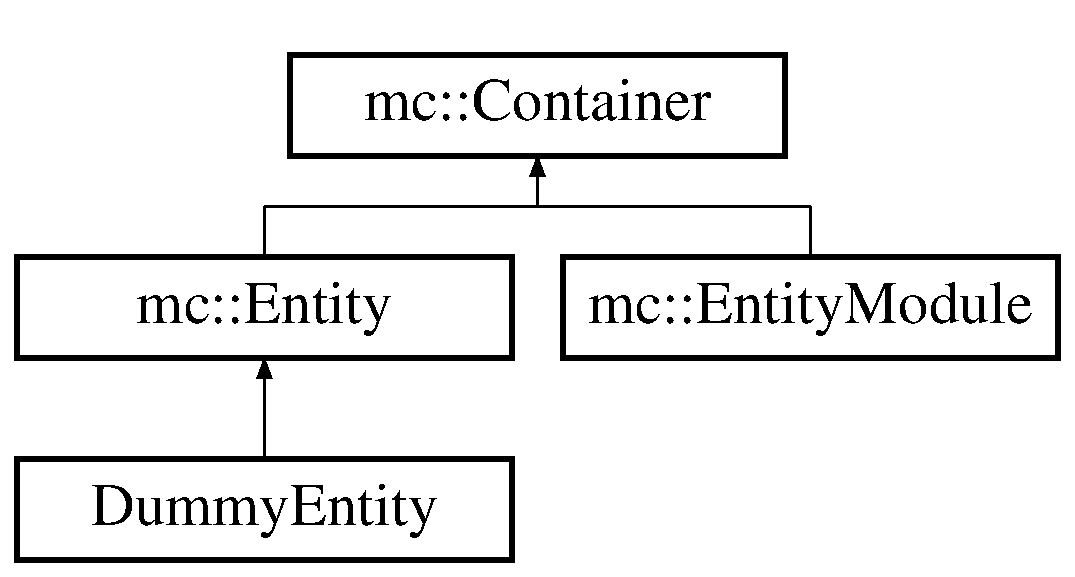
\includegraphics[height=3.000000cm]{classmc_1_1_container}
\end{center}
\end{figure}
\subsection*{Public Member Functions}
\begin{DoxyCompactItemize}
\item 
virtual \hyperlink{classmc_1_1_container_ae9a0af1e1ea151ba9f5654b4f3a5494b}{$\sim$\+Container} ()
\item 
virtual \hyperlink{_s_d_l__opengles2__gl2ext_8h_ae5d8fa23ad07c48bb609509eae494c95}{void} \hyperlink{classmc_1_1_container_a306bb7d15cee23ff8bef4b9342ed85cf}{update} ()
\item 
virtual \hyperlink{_s_d_l__opengles2__gl2ext_8h_ae5d8fa23ad07c48bb609509eae494c95}{void} \hyperlink{classmc_1_1_container_a087d26907d06163aa731d9a313163b7f}{init} ()
\item 
virtual \hyperlink{_s_d_l__opengles2__gl2ext_8h_ae5d8fa23ad07c48bb609509eae494c95}{void} \hyperlink{classmc_1_1_container_a80bd71e4e12ec218e4de88f4e48cc771}{destroy} ()
\item 
const std\+::vector$<$ \hyperlink{classmc_1_1_entity}{Entity} $\ast$ $>$ \& \hyperlink{classmc_1_1_container_a2455ff127249ab0b128fe54eeeaf72e3}{get\+Children} () const 
\item 
\hyperlink{_s_d_l__opengles2__gl2ext_8h_ae5d8fa23ad07c48bb609509eae494c95}{void} \hyperlink{classmc_1_1_container_a7de8a7bfe45c8a869149de774019e42c}{add\+Child} (\hyperlink{classmc_1_1_entity}{Entity} \&e)
\item 
\hyperlink{_s_d_l__opengles2__gl2ext_8h_ae5d8fa23ad07c48bb609509eae494c95}{void} \hyperlink{classmc_1_1_container_ab11d68dc07cd15d6a8a30f63fb8aaa62}{remove\+Child} (const \hyperlink{classmc_1_1_entity}{Entity} \&e)
\item 
\hyperlink{_s_d_l__opengles2__gl2ext_8h_ae5d8fa23ad07c48bb609509eae494c95}{void} \hyperlink{classmc_1_1_container_a2a20247458c80d432a9c7d80f11a15ff}{remove\+Child} (unsigned \hyperlink{_s_d_l__thread_8h_a6a64f9be4433e4de6e2f2f548cf3c08e}{int} \hyperlink{_s_d_l__opengl__glext_8h_a57f14e05b1900f16a2da82ade47d0c6d}{index})
\item 
bool \hyperlink{classmc_1_1_container_a0f947d9066f457d37defd9382da99128}{has\+Child} (\hyperlink{classmc_1_1_entity}{Entity} \&e) const 
\item 
\hyperlink{_s_d_l__opengles2__gl2ext_8h_ae5d8fa23ad07c48bb609509eae494c95}{void} \hyperlink{classmc_1_1_container_aee8b37e3cb3ef52d2b3aee2310007f39}{clear\+Children} ()
\item 
\hyperlink{classmc_1_1_entity}{Entity} \& \hyperlink{classmc_1_1_container_a4d9c9836fca7685c9e3fd314cb2ef3e4}{operator\mbox{[}$\,$\mbox{]}} (unsigned \hyperlink{_s_d_l__thread_8h_a6a64f9be4433e4de6e2f2f548cf3c08e}{int} i)
\item 
const \hyperlink{classmc_1_1_entity}{Entity} \& \hyperlink{classmc_1_1_container_a9a7c43110b0b08ac5edbbfd0a668abe0}{operator\mbox{[}$\,$\mbox{]}} (unsigned \hyperlink{_s_d_l__thread_8h_a6a64f9be4433e4de6e2f2f548cf3c08e}{int} i) const 
\item 
\hyperlink{classmc_1_1_entity}{Entity} \& \hyperlink{classmc_1_1_container_a0f7ec1b14def81f1fbc4e534b7cff8be}{get\+Child} (unsigned \hyperlink{_s_d_l__thread_8h_a6a64f9be4433e4de6e2f2f548cf3c08e}{int} i)
\item 
const \hyperlink{classmc_1_1_entity}{Entity} \& \hyperlink{classmc_1_1_container_af5953e37ee8a9c24a4541e81502e9639}{get\+Child} (unsigned \hyperlink{_s_d_l__thread_8h_a6a64f9be4433e4de6e2f2f548cf3c08e}{int} i) const 
\item 
unsigned \hyperlink{_s_d_l__thread_8h_a6a64f9be4433e4de6e2f2f548cf3c08e}{int} \hyperlink{classmc_1_1_container_ac3b24eb59ccbca4290d032c07eb3e5f6}{index\+Of} (\hyperlink{classmc_1_1_entity}{Entity} \&e) const 
\item 
std\+::vector$<$ \hyperlink{classmc_1_1_entity}{Entity} $\ast$ $>$\+::iterator \hyperlink{classmc_1_1_container_a2838fe4f6068eba635df99b8180a63a1}{begin} ()
\item 
std\+::vector$<$ \hyperlink{classmc_1_1_entity}{Entity} $\ast$ $>$\+::iterator \hyperlink{classmc_1_1_container_af8ce53fdca38afc0c38fd8dc5c7de93d}{end} ()
\item 
\hyperlink{namespacemc_ad1c06461067735b3b17e0df612532c4e}{Size} \hyperlink{classmc_1_1_container_afcba0b879415347bffedde8b43fbce8a}{size} () const 
\item 
bool \hyperlink{classmc_1_1_container_a0c35995b63b9e4a0dc05208a744b326b}{operator==} (\hyperlink{classmc_1_1_container}{Container} \&other) const 
\item 
bool \hyperlink{classmc_1_1_container_af1787e3b31159afec58ee4fffbcec013}{operator!=} (\hyperlink{classmc_1_1_container}{Container} \&other) const 
\end{DoxyCompactItemize}
\subsection*{Protected Attributes}
\begin{DoxyCompactItemize}
\item 
std\+::vector$<$ \hyperlink{classmc_1_1_entity}{Entity} $\ast$ $>$ \hyperlink{classmc_1_1_container_a61ab3823bf33ae5f8f1bfdb79501b242}{children} = std\+::vector$<$\hyperlink{classmc_1_1_entity}{Entity}$\ast$$>$()
\end{DoxyCompactItemize}
\subsection*{Friends}
\begin{DoxyCompactItemize}
\item 
class \hyperlink{classmc_1_1_container_a8dbbff2e42cb66216ff15cfa5272a1c9}{Entity\+Module}
\item 
class \hyperlink{classmc_1_1_container_a614439ccac0344926adc4c0165d64060}{Entity}
\end{DoxyCompactItemize}


\subsection{Detailed Description}
A class which holds an internal buffer of \hyperlink{classmc_1_1_entity}{entities,} known as \char`\"{}children.\char`\"{} 

Calling \hyperlink{classmc_1_1_container_a306bb7d15cee23ff8bef4b9342ed85cf}{update()} will call \hyperlink{}{Entity\#update()} on all of it\textquotesingle{}s children. 

\subsection{Constructor \& Destructor Documentation}
\index{mc\+::\+Container@{mc\+::\+Container}!````~Container@{$\sim$\+Container}}
\index{````~Container@{$\sim$\+Container}!mc\+::\+Container@{mc\+::\+Container}}
\subsubsection[{\texorpdfstring{$\sim$\+Container()}{~Container()}}]{\setlength{\rightskip}{0pt plus 5cm}mc\+::\+Container\+::$\sim$\+Container (
\begin{DoxyParamCaption}
{}
\end{DoxyParamCaption}
)\hspace{0.3cm}{\ttfamily [virtual]}}\hypertarget{classmc_1_1_container_ae9a0af1e1ea151ba9f5654b4f3a5494b}{}\label{classmc_1_1_container_ae9a0af1e1ea151ba9f5654b4f3a5494b}
Destructor. Clears all of the children. \begin{DoxySeeAlso}{See also}
\hyperlink{classmc_1_1_container_aee8b37e3cb3ef52d2b3aee2310007f39}{clear\+Children} 
\end{DoxySeeAlso}


\subsection{Member Function Documentation}
\index{mc\+::\+Container@{mc\+::\+Container}!add\+Child@{add\+Child}}
\index{add\+Child@{add\+Child}!mc\+::\+Container@{mc\+::\+Container}}
\subsubsection[{\texorpdfstring{add\+Child(\+Entity \&e)}{addChild(Entity &e)}}]{\setlength{\rightskip}{0pt plus 5cm}{\bf void} mc\+::\+Container\+::add\+Child (
\begin{DoxyParamCaption}
\item[{{\bf Entity} \&}]{e}
\end{DoxyParamCaption}
)}\hypertarget{classmc_1_1_container_a7de8a7bfe45c8a869149de774019e42c}{}\label{classmc_1_1_container_a7de8a7bfe45c8a869149de774019e42c}
Add an \hyperlink{classmc_1_1_entity}{Entity} to this \hyperlink{classmc_1_1_container}{Container} 
\begin{DoxyParams}{Parameters}
{\em e} & Reference to an
\begin{DoxyCode}
\hyperlink{classmc_1_1_container_a614439ccac0344926adc4c0165d64060}{Entity} 
\end{DoxyCode}
 to become a child \\
\hline
\end{DoxyParams}
\begin{DoxySeeAlso}{See also}
\hyperlink{classmc_1_1_container_a306bb7d15cee23ff8bef4b9342ed85cf}{update()} 

\hyperlink{classmc_1_1_container_a2455ff127249ab0b128fe54eeeaf72e3}{get\+Children()} 
\end{DoxySeeAlso}
\index{mc\+::\+Container@{mc\+::\+Container}!begin@{begin}}
\index{begin@{begin}!mc\+::\+Container@{mc\+::\+Container}}
\subsubsection[{\texorpdfstring{begin()}{begin()}}]{\setlength{\rightskip}{0pt plus 5cm}std\+::vector$<$ {\bf Entity} $\ast$ $>$\+::iterator mc\+::\+Container\+::begin (
\begin{DoxyParamCaption}
{}
\end{DoxyParamCaption}
)}\hypertarget{classmc_1_1_container_a2838fe4f6068eba635df99b8180a63a1}{}\label{classmc_1_1_container_a2838fe4f6068eba635df99b8180a63a1}
\index{mc\+::\+Container@{mc\+::\+Container}!clear\+Children@{clear\+Children}}
\index{clear\+Children@{clear\+Children}!mc\+::\+Container@{mc\+::\+Container}}
\subsubsection[{\texorpdfstring{clear\+Children()}{clearChildren()}}]{\setlength{\rightskip}{0pt plus 5cm}{\bf void} mc\+::\+Container\+::clear\+Children (
\begin{DoxyParamCaption}
{}
\end{DoxyParamCaption}
)}\hypertarget{classmc_1_1_container_aee8b37e3cb3ef52d2b3aee2310007f39}{}\label{classmc_1_1_container_aee8b37e3cb3ef52d2b3aee2310007f39}
Removes E\+V\+E\+RY \{code \hyperlink{classmc_1_1_entity}{Entity}\} from this
\begin{DoxyCode}
Container. 
\end{DoxyCode}
 \begin{DoxySeeAlso}{See also}
\hyperlink{classmc_1_1_container_afcba0b879415347bffedde8b43fbce8a}{size()} 

\hyperlink{classmc_1_1_container_a2a20247458c80d432a9c7d80f11a15ff}{remove\+Child(unsigned int)} 

\hyperlink{classmc_1_1_container_ab11d68dc07cd15d6a8a30f63fb8aaa62}{remove\+Child(const Entity\&)} 
\end{DoxySeeAlso}
\index{mc\+::\+Container@{mc\+::\+Container}!destroy@{destroy}}
\index{destroy@{destroy}!mc\+::\+Container@{mc\+::\+Container}}
\subsubsection[{\texorpdfstring{destroy()}{destroy()}}]{\setlength{\rightskip}{0pt plus 5cm}{\bf void} mc\+::\+Container\+::destroy (
\begin{DoxyParamCaption}
{}
\end{DoxyParamCaption}
)\hspace{0.3cm}{\ttfamily [virtual]}}\hypertarget{classmc_1_1_container_a80bd71e4e12ec218e4de88f4e48cc771}{}\label{classmc_1_1_container_a80bd71e4e12ec218e4de88f4e48cc771}
Should be called every time \hyperlink{}{System\#destroy()} is called. Calls
\begin{DoxyCode}
\hyperlink{classmc_1_1_container_a80bd71e4e12ec218e4de88f4e48cc771}{destroy}() 
\end{DoxyCode}
 on all of this
\begin{DoxyCode}
Container\textcolor{stringliteral}{'s }
\end{DoxyCode}
 children. 

Reimplemented in \hyperlink{classmc_1_1_entity_module_a6c0fe0216850bb703df6721940f78b5f}{mc\+::\+Entity\+Module}.

\index{mc\+::\+Container@{mc\+::\+Container}!end@{end}}
\index{end@{end}!mc\+::\+Container@{mc\+::\+Container}}
\subsubsection[{\texorpdfstring{end()}{end()}}]{\setlength{\rightskip}{0pt plus 5cm}std\+::vector$<$ {\bf Entity} $\ast$ $>$\+::iterator mc\+::\+Container\+::end (
\begin{DoxyParamCaption}
{}
\end{DoxyParamCaption}
)}\hypertarget{classmc_1_1_container_af8ce53fdca38afc0c38fd8dc5c7de93d}{}\label{classmc_1_1_container_af8ce53fdca38afc0c38fd8dc5c7de93d}
\index{mc\+::\+Container@{mc\+::\+Container}!get\+Child@{get\+Child}}
\index{get\+Child@{get\+Child}!mc\+::\+Container@{mc\+::\+Container}}
\subsubsection[{\texorpdfstring{get\+Child(unsigned int i)}{getChild(unsigned int i)}}]{\setlength{\rightskip}{0pt plus 5cm}{\bf Entity} \& mc\+::\+Container\+::get\+Child (
\begin{DoxyParamCaption}
\item[{unsigned {\bf int}}]{i}
\end{DoxyParamCaption}
)}\hypertarget{classmc_1_1_container_a0f7ec1b14def81f1fbc4e534b7cff8be}{}\label{classmc_1_1_container_a0f7ec1b14def81f1fbc4e534b7cff8be}
\index{mc\+::\+Container@{mc\+::\+Container}!get\+Child@{get\+Child}}
\index{get\+Child@{get\+Child}!mc\+::\+Container@{mc\+::\+Container}}
\subsubsection[{\texorpdfstring{get\+Child(unsigned int i) const }{getChild(unsigned int i) const }}]{\setlength{\rightskip}{0pt plus 5cm}const {\bf Entity} \& mc\+::\+Container\+::get\+Child (
\begin{DoxyParamCaption}
\item[{unsigned {\bf int}}]{i}
\end{DoxyParamCaption}
) const}\hypertarget{classmc_1_1_container_af5953e37ee8a9c24a4541e81502e9639}{}\label{classmc_1_1_container_af5953e37ee8a9c24a4541e81502e9639}
\index{mc\+::\+Container@{mc\+::\+Container}!get\+Children@{get\+Children}}
\index{get\+Children@{get\+Children}!mc\+::\+Container@{mc\+::\+Container}}
\subsubsection[{\texorpdfstring{get\+Children() const }{getChildren() const }}]{\setlength{\rightskip}{0pt plus 5cm}const std\+::vector$<$ {\bf Entity} $\ast$ $>$ \& mc\+::\+Container\+::get\+Children (
\begin{DoxyParamCaption}
{}
\end{DoxyParamCaption}
) const}\hypertarget{classmc_1_1_container_a2455ff127249ab0b128fe54eeeaf72e3}{}\label{classmc_1_1_container_a2455ff127249ab0b128fe54eeeaf72e3}
Gets all of this
\begin{DoxyCode}
Container\textcolor{stringliteral}{'s }
\end{DoxyCode}
 children. \begin{DoxyReturn}{Returns}
an
\begin{DoxyCode}
std::vector 
\end{DoxyCode}
 with all children of this
\begin{DoxyCode}
Container 
\end{DoxyCode}
 
\end{DoxyReturn}
\index{mc\+::\+Container@{mc\+::\+Container}!has\+Child@{has\+Child}}
\index{has\+Child@{has\+Child}!mc\+::\+Container@{mc\+::\+Container}}
\subsubsection[{\texorpdfstring{has\+Child(\+Entity \&e) const }{hasChild(Entity &e) const }}]{\setlength{\rightskip}{0pt plus 5cm}bool mc\+::\+Container\+::has\+Child (
\begin{DoxyParamCaption}
\item[{{\bf Entity} \&}]{e}
\end{DoxyParamCaption}
) const}\hypertarget{classmc_1_1_container_a0f947d9066f457d37defd9382da99128}{}\label{classmc_1_1_container_a0f947d9066f457d37defd9382da99128}
Checks to see if this
\begin{DoxyCode}
Container 
\end{DoxyCode}
 contains an
\begin{DoxyCode}
\hyperlink{classmc_1_1_container_a614439ccac0344926adc4c0165d64060}{Entity} 
\end{DoxyCode}
 
\begin{DoxyParams}{Parameters}
{\em e} & Reference to an
\begin{DoxyCode}
\hyperlink{classmc_1_1_container_a614439ccac0344926adc4c0165d64060}{Entity} 
\end{DoxyCode}
 \\
\hline
\end{DoxyParams}
\begin{DoxyReturn}{Returns}

\begin{DoxyCode}
\textcolor{keyword}{false} 
\end{DoxyCode}
 if this
\begin{DoxyCode}
Container 
\end{DoxyCode}
 doesn\textquotesingle{}t contain the referenced
\begin{DoxyCode}
\hyperlink{classmc_1_1_container_a614439ccac0344926adc4c0165d64060}{Entity}, \textcolor{keyword}{true} 
\end{DoxyCode}
 
\end{DoxyReturn}
\begin{DoxySeeAlso}{See also}
\#index\+Of(\+Entity\& ) 
\end{DoxySeeAlso}
\index{mc\+::\+Container@{mc\+::\+Container}!index\+Of@{index\+Of}}
\index{index\+Of@{index\+Of}!mc\+::\+Container@{mc\+::\+Container}}
\subsubsection[{\texorpdfstring{index\+Of(\+Entity \&e) const }{indexOf(Entity &e) const }}]{\setlength{\rightskip}{0pt plus 5cm}unsigned {\bf int} mc\+::\+Container\+::index\+Of (
\begin{DoxyParamCaption}
\item[{{\bf Entity} \&}]{e}
\end{DoxyParamCaption}
) const}\hypertarget{classmc_1_1_container_ac3b24eb59ccbca4290d032c07eb3e5f6}{}\label{classmc_1_1_container_ac3b24eb59ccbca4290d032c07eb3e5f6}
\index{mc\+::\+Container@{mc\+::\+Container}!init@{init}}
\index{init@{init}!mc\+::\+Container@{mc\+::\+Container}}
\subsubsection[{\texorpdfstring{init()}{init()}}]{\setlength{\rightskip}{0pt plus 5cm}{\bf void} mc\+::\+Container\+::init (
\begin{DoxyParamCaption}
{}
\end{DoxyParamCaption}
)\hspace{0.3cm}{\ttfamily [virtual]}}\hypertarget{classmc_1_1_container_a087d26907d06163aa731d9a313163b7f}{}\label{classmc_1_1_container_a087d26907d06163aa731d9a313163b7f}
Should be called every time \hyperlink{classmc_1_1_system_a86b7559895967af432c5c3db728bd0bc}{System\#init()} is called. Calls
\begin{DoxyCode}
\hyperlink{classmc_1_1_container_a087d26907d06163aa731d9a313163b7f}{init}() 
\end{DoxyCode}
 on all of this
\begin{DoxyCode}
Container\textcolor{stringliteral}{'s }
\end{DoxyCode}
 children. 

Reimplemented in \hyperlink{classmc_1_1_entity_module_a5e1f25e0d12c50f6e8d8fbdf31028b8e}{mc\+::\+Entity\+Module}.

\index{mc\+::\+Container@{mc\+::\+Container}!operator"!=@{operator"!=}}
\index{operator"!=@{operator"!=}!mc\+::\+Container@{mc\+::\+Container}}
\subsubsection[{\texorpdfstring{operator"!=(\+Container \&other) const }{operator!=(Container &other) const }}]{\setlength{\rightskip}{0pt plus 5cm}bool mc\+::\+Container\+::operator!= (
\begin{DoxyParamCaption}
\item[{{\bf Container} \&}]{other}
\end{DoxyParamCaption}
) const}\hypertarget{classmc_1_1_container_af1787e3b31159afec58ee4fffbcec013}{}\label{classmc_1_1_container_af1787e3b31159afec58ee4fffbcec013}
\index{mc\+::\+Container@{mc\+::\+Container}!operator==@{operator==}}
\index{operator==@{operator==}!mc\+::\+Container@{mc\+::\+Container}}
\subsubsection[{\texorpdfstring{operator==(\+Container \&other) const }{operator==(Container &other) const }}]{\setlength{\rightskip}{0pt plus 5cm}bool mc\+::\+Container\+::operator== (
\begin{DoxyParamCaption}
\item[{{\bf Container} \&}]{other}
\end{DoxyParamCaption}
) const}\hypertarget{classmc_1_1_container_a0c35995b63b9e4a0dc05208a744b326b}{}\label{classmc_1_1_container_a0c35995b63b9e4a0dc05208a744b326b}
\index{mc\+::\+Container@{mc\+::\+Container}!operator\mbox{[}$\,$\mbox{]}@{operator[]}}
\index{operator\mbox{[}$\,$\mbox{]}@{operator[]}!mc\+::\+Container@{mc\+::\+Container}}
\subsubsection[{\texorpdfstring{operator[](unsigned int i)}{operator[](unsigned int i)}}]{\setlength{\rightskip}{0pt plus 5cm}{\bf Entity} \& mc\+::\+Container\+::operator\mbox{[}$\,$\mbox{]} (
\begin{DoxyParamCaption}
\item[{unsigned {\bf int}}]{i}
\end{DoxyParamCaption}
)}\hypertarget{classmc_1_1_container_a4d9c9836fca7685c9e3fd314cb2ef3e4}{}\label{classmc_1_1_container_a4d9c9836fca7685c9e3fd314cb2ef3e4}
Access an
\begin{DoxyCode}
\hyperlink{classmc_1_1_container_a614439ccac0344926adc4c0165d64060}{Entity} 
\end{DoxyCode}
 . \begin{DoxySeeAlso}{See also}
\hyperlink{classmc_1_1_container_a0f7ec1b14def81f1fbc4e534b7cff8be}{get\+Child(unsigned int)} 
\end{DoxySeeAlso}
\index{mc\+::\+Container@{mc\+::\+Container}!operator\mbox{[}$\,$\mbox{]}@{operator[]}}
\index{operator\mbox{[}$\,$\mbox{]}@{operator[]}!mc\+::\+Container@{mc\+::\+Container}}
\subsubsection[{\texorpdfstring{operator[](unsigned int i) const }{operator[](unsigned int i) const }}]{\setlength{\rightskip}{0pt plus 5cm}const {\bf Entity} \& mc\+::\+Container\+::operator\mbox{[}$\,$\mbox{]} (
\begin{DoxyParamCaption}
\item[{unsigned {\bf int}}]{i}
\end{DoxyParamCaption}
) const}\hypertarget{classmc_1_1_container_a9a7c43110b0b08ac5edbbfd0a668abe0}{}\label{classmc_1_1_container_a9a7c43110b0b08ac5edbbfd0a668abe0}
\index{mc\+::\+Container@{mc\+::\+Container}!remove\+Child@{remove\+Child}}
\index{remove\+Child@{remove\+Child}!mc\+::\+Container@{mc\+::\+Container}}
\subsubsection[{\texorpdfstring{remove\+Child(const Entity \&e)}{removeChild(const Entity &e)}}]{\setlength{\rightskip}{0pt plus 5cm}{\bf void} mc\+::\+Container\+::remove\+Child (
\begin{DoxyParamCaption}
\item[{const {\bf Entity} \&}]{e}
\end{DoxyParamCaption}
)}\hypertarget{classmc_1_1_container_ab11d68dc07cd15d6a8a30f63fb8aaa62}{}\label{classmc_1_1_container_ab11d68dc07cd15d6a8a30f63fb8aaa62}
Removes a child by reference.


\begin{DoxyExceptions}{Exceptions}
{\em } & \\
\hline
\end{DoxyExceptions}
\index{mc\+::\+Container@{mc\+::\+Container}!remove\+Child@{remove\+Child}}
\index{remove\+Child@{remove\+Child}!mc\+::\+Container@{mc\+::\+Container}}
\subsubsection[{\texorpdfstring{remove\+Child(unsigned int index)}{removeChild(unsigned int index)}}]{\setlength{\rightskip}{0pt plus 5cm}{\bf void} mc\+::\+Container\+::remove\+Child (
\begin{DoxyParamCaption}
\item[{unsigned {\bf int}}]{index}
\end{DoxyParamCaption}
)}\hypertarget{classmc_1_1_container_a2a20247458c80d432a9c7d80f11a15ff}{}\label{classmc_1_1_container_a2a20247458c80d432a9c7d80f11a15ff}
Removes a child via location.


\begin{DoxyExceptions}{Exceptions}
{\em } & \\
\hline
\end{DoxyExceptions}
\index{mc\+::\+Container@{mc\+::\+Container}!size@{size}}
\index{size@{size}!mc\+::\+Container@{mc\+::\+Container}}
\subsubsection[{\texorpdfstring{size() const }{size() const }}]{\setlength{\rightskip}{0pt plus 5cm}{\bf Size} mc\+::\+Container\+::size (
\begin{DoxyParamCaption}
{}
\end{DoxyParamCaption}
) const}\hypertarget{classmc_1_1_container_afcba0b879415347bffedde8b43fbce8a}{}\label{classmc_1_1_container_afcba0b879415347bffedde8b43fbce8a}
\index{mc\+::\+Container@{mc\+::\+Container}!update@{update}}
\index{update@{update}!mc\+::\+Container@{mc\+::\+Container}}
\subsubsection[{\texorpdfstring{update()}{update()}}]{\setlength{\rightskip}{0pt plus 5cm}{\bf void} mc\+::\+Container\+::update (
\begin{DoxyParamCaption}
{}
\end{DoxyParamCaption}
)\hspace{0.3cm}{\ttfamily [virtual]}}\hypertarget{classmc_1_1_container_a306bb7d15cee23ff8bef4b9342ed85cf}{}\label{classmc_1_1_container_a306bb7d15cee23ff8bef4b9342ed85cf}
Should be called every time \hyperlink{classmc_1_1_system_a90e14e44eb5a6019c913a6a197deb4a0}{System\#update()} is called. Calls
\begin{DoxyCode}
\hyperlink{classmc_1_1_container_a306bb7d15cee23ff8bef4b9342ed85cf}{update}() 
\end{DoxyCode}
 on all of this
\begin{DoxyCode}
Container\textcolor{stringliteral}{'s }
\end{DoxyCode}
 children. 

Reimplemented in \hyperlink{classmc_1_1_entity_module_a3307eb2ce5af81b6a6e26fdaa12e3063}{mc\+::\+Entity\+Module}.



\subsection{Friends And Related Function Documentation}
\index{mc\+::\+Container@{mc\+::\+Container}!Entity@{Entity}}
\index{Entity@{Entity}!mc\+::\+Container@{mc\+::\+Container}}
\subsubsection[{\texorpdfstring{Entity}{Entity}}]{\setlength{\rightskip}{0pt plus 5cm}friend class {\bf Entity}\hspace{0.3cm}{\ttfamily [friend]}}\hypertarget{classmc_1_1_container_a614439ccac0344926adc4c0165d64060}{}\label{classmc_1_1_container_a614439ccac0344926adc4c0165d64060}
\index{mc\+::\+Container@{mc\+::\+Container}!Entity\+Module@{Entity\+Module}}
\index{Entity\+Module@{Entity\+Module}!mc\+::\+Container@{mc\+::\+Container}}
\subsubsection[{\texorpdfstring{Entity\+Module}{EntityModule}}]{\setlength{\rightskip}{0pt plus 5cm}friend class {\bf Entity\+Module}\hspace{0.3cm}{\ttfamily [friend]}}\hypertarget{classmc_1_1_container_a8dbbff2e42cb66216ff15cfa5272a1c9}{}\label{classmc_1_1_container_a8dbbff2e42cb66216ff15cfa5272a1c9}


\subsection{Member Data Documentation}
\index{mc\+::\+Container@{mc\+::\+Container}!children@{children}}
\index{children@{children}!mc\+::\+Container@{mc\+::\+Container}}
\subsubsection[{\texorpdfstring{children}{children}}]{\setlength{\rightskip}{0pt plus 5cm}std\+::vector$<${\bf Entity}$\ast$$>$ mc\+::\+Container\+::children = std\+::vector$<${\bf Entity}$\ast$$>$()\hspace{0.3cm}{\ttfamily [protected]}}\hypertarget{classmc_1_1_container_a61ab3823bf33ae5f8f1bfdb79501b242}{}\label{classmc_1_1_container_a61ab3823bf33ae5f8f1bfdb79501b242}


The documentation for this class was generated from the following files\+:\begin{DoxyCompactItemize}
\item 
D\+:/\+Workspace/\+M\+A\+C\+E/\+M\+C-\/\+System/\+Entities/\hyperlink{_entity_8h}{Entity.\+h}\item 
D\+:/\+Workspace/\+M\+A\+C\+E/\+M\+C-\/\+System/\+Entities/\hyperlink{_entity_8cpp}{Entity.\+cpp}\end{DoxyCompactItemize}

\hypertarget{structmc_1_1_dependency_not_found}{}\section{mc\+:\+:Dependency\+Not\+Found Struct Reference}
\label{structmc_1_1_dependency_not_found}\index{mc\+::\+Dependency\+Not\+Found@{mc\+::\+Dependency\+Not\+Found}}


{\ttfamily \#include $<$Exceptions.\+h$>$}

Inheritance diagram for mc\+:\+:Dependency\+Not\+Found\+:\begin{figure}[H]
\begin{center}
\leavevmode
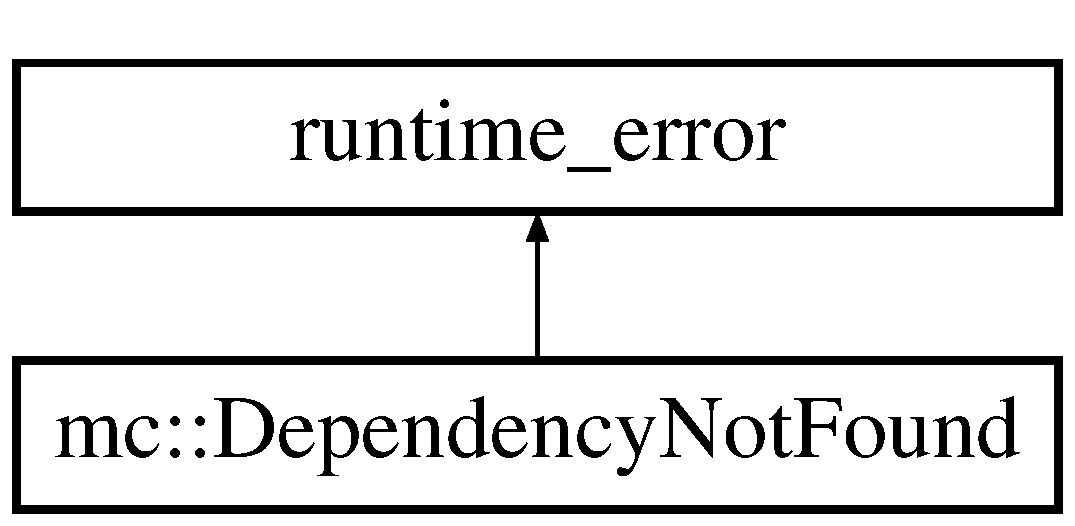
\includegraphics[height=2.000000cm]{structmc_1_1_dependency_not_found}
\end{center}
\end{figure}
\subsection*{Public Member Functions}
\begin{DoxyCompactItemize}
\item 
\hyperlink{structmc_1_1_dependency_not_found_a273e86336a035aff0589b7f76cb70e57}{Dependency\+Not\+Found} (const char $\ast$\hyperlink{_s_d_l__opengl__glext_8h_a1f2d7f8147412c43ba2303a56f97ee73}{c}=\char`\"{}No \hyperlink{_s_d_l__opengl__glext_8h_a7b6161cffb9b8aee272b3b916183d28c}{message} was given\char`\"{})
\item 
\hyperlink{structmc_1_1_dependency_not_found_a0c92690d1b7e523117887a0772ee155d}{Dependency\+Not\+Found} (const \hyperlink{_s_d_l__opengl__glext_8h_ae84541b4f3d8e1ea24ec0f466a8c568b}{std\+::string} \hyperlink{_s_d_l__opengl__glext_8h_a1f2d7f8147412c43ba2303a56f97ee73}{c}=\char`\"{}No \hyperlink{_s_d_l__opengl__glext_8h_a7b6161cffb9b8aee272b3b916183d28c}{message} was given\char`\"{})
\end{DoxyCompactItemize}


\subsection{Constructor \& Destructor Documentation}
\index{mc\+::\+Dependency\+Not\+Found@{mc\+::\+Dependency\+Not\+Found}!Dependency\+Not\+Found@{Dependency\+Not\+Found}}
\index{Dependency\+Not\+Found@{Dependency\+Not\+Found}!mc\+::\+Dependency\+Not\+Found@{mc\+::\+Dependency\+Not\+Found}}
\subsubsection[{\texorpdfstring{Dependency\+Not\+Found(const char $\ast$c=""No message was given"")}{DependencyNotFound(const char *c="No message was given")}}]{\setlength{\rightskip}{0pt plus 5cm}mc\+::\+Dependency\+Not\+Found\+::\+Dependency\+Not\+Found (
\begin{DoxyParamCaption}
\item[{const char $\ast$}]{c = {\ttfamily \char`\"{}No~{\bf message}~was~given\char`\"{}}}
\end{DoxyParamCaption}
)\hspace{0.3cm}{\ttfamily [inline]}, {\ttfamily [explicit]}}\hypertarget{structmc_1_1_dependency_not_found_a273e86336a035aff0589b7f76cb70e57}{}\label{structmc_1_1_dependency_not_found_a273e86336a035aff0589b7f76cb70e57}
\index{mc\+::\+Dependency\+Not\+Found@{mc\+::\+Dependency\+Not\+Found}!Dependency\+Not\+Found@{Dependency\+Not\+Found}}
\index{Dependency\+Not\+Found@{Dependency\+Not\+Found}!mc\+::\+Dependency\+Not\+Found@{mc\+::\+Dependency\+Not\+Found}}
\subsubsection[{\texorpdfstring{Dependency\+Not\+Found(const std\+::string c=""No message was given"")}{DependencyNotFound(const std::string c="No message was given")}}]{\setlength{\rightskip}{0pt plus 5cm}mc\+::\+Dependency\+Not\+Found\+::\+Dependency\+Not\+Found (
\begin{DoxyParamCaption}
\item[{const {\bf std\+::string}}]{c = {\ttfamily \char`\"{}No~{\bf message}~was~given\char`\"{}}}
\end{DoxyParamCaption}
)\hspace{0.3cm}{\ttfamily [inline]}, {\ttfamily [explicit]}}\hypertarget{structmc_1_1_dependency_not_found_a0c92690d1b7e523117887a0772ee155d}{}\label{structmc_1_1_dependency_not_found_a0c92690d1b7e523117887a0772ee155d}


The documentation for this struct was generated from the following file\+:\begin{DoxyCompactItemize}
\item 
D\+:/\+Workspace/\+M\+A\+C\+E/\+M\+C-\/\+System/\hyperlink{_exceptions_8h}{Exceptions.\+h}\end{DoxyCompactItemize}

\hypertarget{classmc_1_1_entity}{}\section{mc\+:\+:Entity Class Reference}
\label{classmc_1_1_entity}\index{mc\+::\+Entity@{mc\+::\+Entity}}


{\ttfamily \#include $<$Entity.\+h$>$}

Inheritance diagram for mc\+:\+:Entity\+:\begin{figure}[H]
\begin{center}
\leavevmode
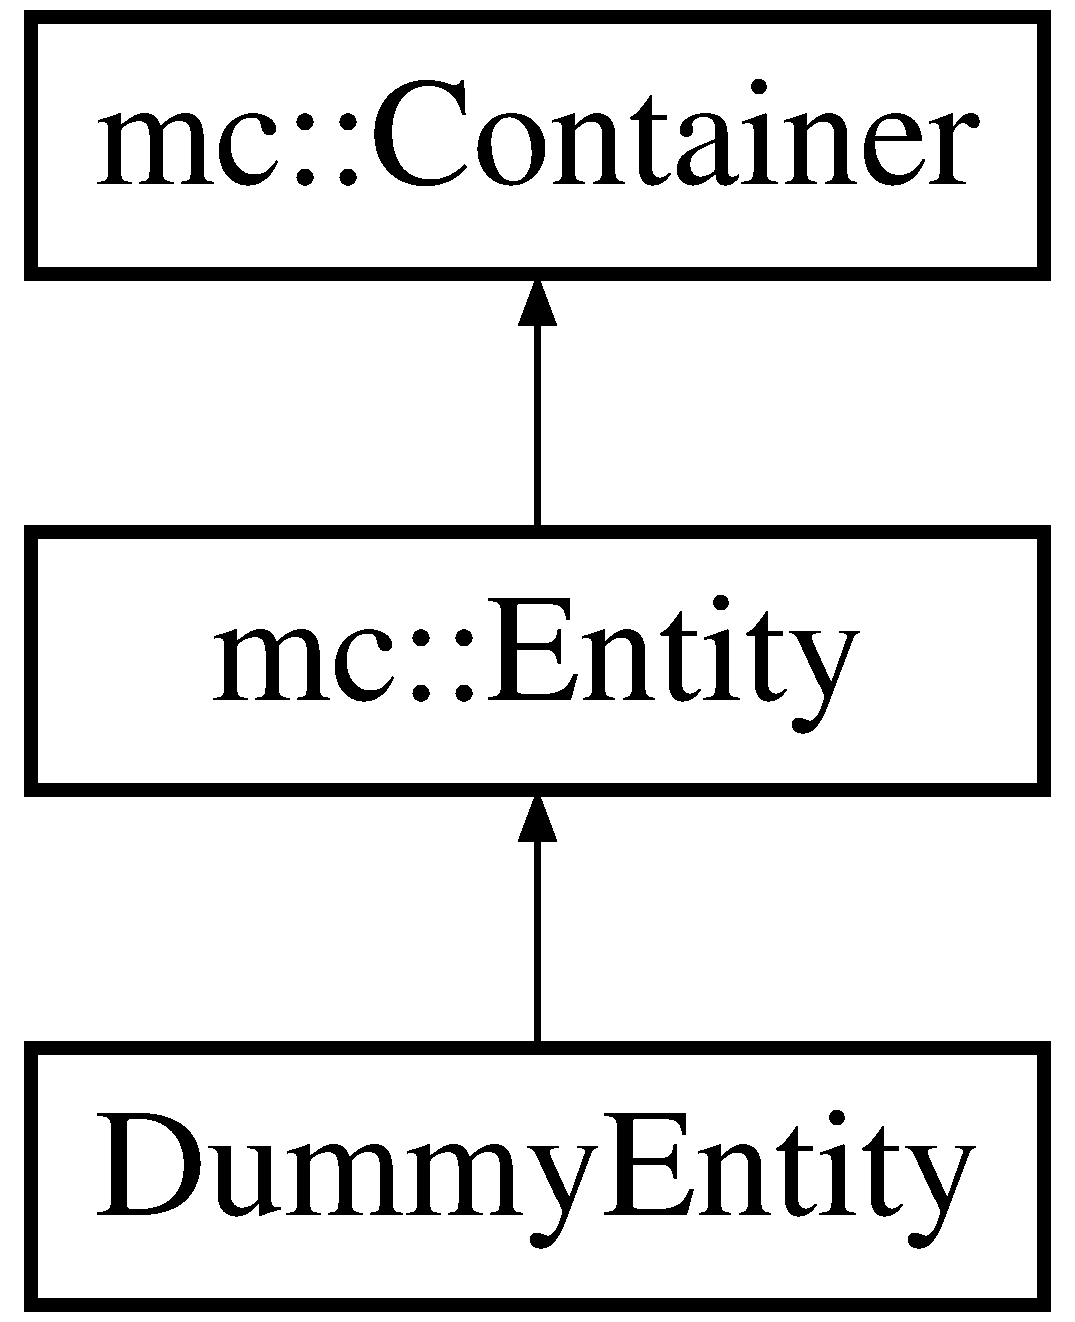
\includegraphics[height=3.000000cm]{classmc_1_1_entity}
\end{center}
\end{figure}
\subsection*{Public Member Functions}
\begin{DoxyCompactItemize}
\item 
\hyperlink{classmc_1_1_entity_ad583efd4016d2c77f6f60507b55fb6f8}{Entity} ()
\item 
\hyperlink{classmc_1_1_entity_a9b3dbd9aef3eb14da2e84a4352546835}{Entity} (const \hyperlink{classmc_1_1_entity}{Entity} \&\hyperlink{_s_d_l__opengl__glext_8h_a0c0d4701a6c89f4f7f0640715d27ab26}{obj})
\item 
virtual \hyperlink{classmc_1_1_entity_a5d546959498cbd99c27c0cd03cc95857}{$\sim$\+Entity} ()
\item 
\hyperlink{namespacemc_a4ed352b00f84d2c3e9843cf5ea375ca0}{Byte\+Field} \& \hyperlink{classmc_1_1_entity_afb7e498851027d6dfe5c6e4dbd2e1364}{get\+Properties} ()
\item 
const \hyperlink{namespacemc_a4ed352b00f84d2c3e9843cf5ea375ca0}{Byte\+Field} \& \hyperlink{classmc_1_1_entity_a0e026645818370ea5c5a72817558e89a}{get\+Properties} () const 
\item 
\hyperlink{_s_d_l__opengles2__gl2ext_8h_ae5d8fa23ad07c48bb609509eae494c95}{void} \hyperlink{classmc_1_1_entity_ae644b908a86a45da6d3620897205d942}{set\+Properties} (\hyperlink{namespacemc_a4ed352b00f84d2c3e9843cf5ea375ca0}{Byte\+Field} \&\hyperlink{_s_d_l__opengl__glext_8h_a0f71581a41fd2264c8944126dabbd010}{b})
\item 
bool \hyperlink{classmc_1_1_entity_ace44e845914092b907df3ecaaa50547d}{get\+Property} (unsigned \hyperlink{_s_d_l__thread_8h_a6a64f9be4433e4de6e2f2f548cf3c08e}{int} position) const 
\item 
\hyperlink{_s_d_l__opengles2__gl2ext_8h_ae5d8fa23ad07c48bb609509eae494c95}{void} \hyperlink{classmc_1_1_entity_ad771c3db0dadcd167df40fb04a1c10af}{set\+Property} (unsigned \hyperlink{_s_d_l__thread_8h_a6a64f9be4433e4de6e2f2f548cf3c08e}{int} position, bool \hyperlink{_s_d_l__opengl__glext_8h_a8ad81492d410ff2ac11f754f4042150f}{value})
\item 
const \hyperlink{classmc_1_1_container}{Container} \& \hyperlink{classmc_1_1_entity_a6ca2e4084875e5cde83b7e8b6fc012d3}{get\+Parent} () const 
\item 
\hyperlink{classmc_1_1_container}{Container} \& \hyperlink{classmc_1_1_entity_a1900c874fc79eb246d7ec01198264dc8}{get\+Parent} ()
\item 
bool \hyperlink{classmc_1_1_entity_a7918ed0bd53b9f09a0e57f9312eef4cc}{operator==} (\hyperlink{classmc_1_1_entity}{Entity} \&other) const 
\item 
bool \hyperlink{classmc_1_1_entity_a6cb31e44de7988da15b5e811f160c12d}{operator!=} (\hyperlink{classmc_1_1_entity}{Entity} \&other) const 
\item 
\hyperlink{_s_d_l__opengles2__gl2ext_8h_ae5d8fa23ad07c48bb609509eae494c95}{void} \hyperlink{classmc_1_1_entity_ac627ec2fd2977dee614b96cee332775f}{kill} ()
\end{DoxyCompactItemize}
\subsection*{Static Public Member Functions}
\begin{DoxyCompactItemize}
\item 
static \hyperlink{_s_d_l__opengles2__gl2ext_8h_ae5d8fa23ad07c48bb609509eae494c95}{void} \hyperlink{classmc_1_1_entity_a1db8a8b8c969deedaf12f8892531d8d0}{clean\+Entity} (\hyperlink{classmc_1_1_entity}{Entity} $\ast$e)
\end{DoxyCompactItemize}
\subsection*{Protected Member Functions}
\begin{DoxyCompactItemize}
\item 
virtual \hyperlink{_s_d_l__opengles2__gl2ext_8h_ae5d8fa23ad07c48bb609509eae494c95}{void} \hyperlink{classmc_1_1_entity_af10b82880e3740b7cbb5ed80bb9f6004}{custom\+Update} ()=0
\item 
virtual \hyperlink{_s_d_l__opengles2__gl2ext_8h_ae5d8fa23ad07c48bb609509eae494c95}{void} \hyperlink{classmc_1_1_entity_a6f8fcf75f3b584fc47523110a1c74f39}{custom\+Init} ()=0
\item 
virtual \hyperlink{_s_d_l__opengles2__gl2ext_8h_ae5d8fa23ad07c48bb609509eae494c95}{void} \hyperlink{classmc_1_1_entity_a2f639d91d2f9e933f4769841ad348ddd}{custom\+Destroy} ()=0
\end{DoxyCompactItemize}
\subsection*{Protected Attributes}
\begin{DoxyCompactItemize}
\item 
\hyperlink{namespacemc_a4ed352b00f84d2c3e9843cf5ea375ca0}{Byte\+Field} \hyperlink{classmc_1_1_entity_a4b96da9b66787566c63044472d690da1}{properties} = \hyperlink{namespacemc_aad93bda8c11c45721d4d2feb348f9d5f}{E\+N\+T\+I\+T\+Y\+\_\+\+D\+E\+F\+A\+U\+L\+T\+\_\+\+P\+R\+O\+P\+E\+R\+T\+I\+ES}
\end{DoxyCompactItemize}
\subsection*{Friends}
\begin{DoxyCompactItemize}
\item 
class \hyperlink{classmc_1_1_entity_aee29d97f7e87f0263024133085c28e3d}{Container}
\end{DoxyCompactItemize}


\subsection{Constructor \& Destructor Documentation}
\index{mc\+::\+Entity@{mc\+::\+Entity}!Entity@{Entity}}
\index{Entity@{Entity}!mc\+::\+Entity@{mc\+::\+Entity}}
\subsubsection[{\texorpdfstring{Entity()}{Entity()}}]{\setlength{\rightskip}{0pt plus 5cm}mc\+::\+Entity\+::\+Entity (
\begin{DoxyParamCaption}
{}
\end{DoxyParamCaption}
)}\hypertarget{classmc_1_1_entity_ad583efd4016d2c77f6f60507b55fb6f8}{}\label{classmc_1_1_entity_ad583efd4016d2c77f6f60507b55fb6f8}
\index{mc\+::\+Entity@{mc\+::\+Entity}!Entity@{Entity}}
\index{Entity@{Entity}!mc\+::\+Entity@{mc\+::\+Entity}}
\subsubsection[{\texorpdfstring{Entity(const Entity \&obj)}{Entity(const Entity &obj)}}]{\setlength{\rightskip}{0pt plus 5cm}mc\+::\+Entity\+::\+Entity (
\begin{DoxyParamCaption}
\item[{const {\bf Entity} \&}]{obj}
\end{DoxyParamCaption}
)}\hypertarget{classmc_1_1_entity_a9b3dbd9aef3eb14da2e84a4352546835}{}\label{classmc_1_1_entity_a9b3dbd9aef3eb14da2e84a4352546835}
\index{mc\+::\+Entity@{mc\+::\+Entity}!````~Entity@{$\sim$\+Entity}}
\index{````~Entity@{$\sim$\+Entity}!mc\+::\+Entity@{mc\+::\+Entity}}
\subsubsection[{\texorpdfstring{$\sim$\+Entity()}{~Entity()}}]{\setlength{\rightskip}{0pt plus 5cm}mc\+::\+Entity\+::$\sim$\+Entity (
\begin{DoxyParamCaption}
{}
\end{DoxyParamCaption}
)\hspace{0.3cm}{\ttfamily [virtual]}}\hypertarget{classmc_1_1_entity_a5d546959498cbd99c27c0cd03cc95857}{}\label{classmc_1_1_entity_a5d546959498cbd99c27c0cd03cc95857}


\subsection{Member Function Documentation}
\index{mc\+::\+Entity@{mc\+::\+Entity}!clean\+Entity@{clean\+Entity}}
\index{clean\+Entity@{clean\+Entity}!mc\+::\+Entity@{mc\+::\+Entity}}
\subsubsection[{\texorpdfstring{clean\+Entity(\+Entity $\ast$e)}{cleanEntity(Entity *e)}}]{\setlength{\rightskip}{0pt plus 5cm}{\bf void} mc\+::\+Entity\+::clean\+Entity (
\begin{DoxyParamCaption}
\item[{{\bf Entity} $\ast$}]{e}
\end{DoxyParamCaption}
)\hspace{0.3cm}{\ttfamily [static]}}\hypertarget{classmc_1_1_entity_a1db8a8b8c969deedaf12f8892531d8d0}{}\label{classmc_1_1_entity_a1db8a8b8c969deedaf12f8892531d8d0}
\index{mc\+::\+Entity@{mc\+::\+Entity}!custom\+Destroy@{custom\+Destroy}}
\index{custom\+Destroy@{custom\+Destroy}!mc\+::\+Entity@{mc\+::\+Entity}}
\subsubsection[{\texorpdfstring{custom\+Destroy()=0}{customDestroy()=0}}]{\setlength{\rightskip}{0pt plus 5cm}virtual {\bf void} mc\+::\+Entity\+::custom\+Destroy (
\begin{DoxyParamCaption}
{}
\end{DoxyParamCaption}
)\hspace{0.3cm}{\ttfamily [protected]}, {\ttfamily [pure virtual]}}\hypertarget{classmc_1_1_entity_a2f639d91d2f9e933f4769841ad348ddd}{}\label{classmc_1_1_entity_a2f639d91d2f9e933f4769841ad348ddd}


Implemented in \hyperlink{class_dummy_entity_a9e7c6555400befc5c1d658523c32ac64}{Dummy\+Entity}.

\index{mc\+::\+Entity@{mc\+::\+Entity}!custom\+Init@{custom\+Init}}
\index{custom\+Init@{custom\+Init}!mc\+::\+Entity@{mc\+::\+Entity}}
\subsubsection[{\texorpdfstring{custom\+Init()=0}{customInit()=0}}]{\setlength{\rightskip}{0pt plus 5cm}virtual {\bf void} mc\+::\+Entity\+::custom\+Init (
\begin{DoxyParamCaption}
{}
\end{DoxyParamCaption}
)\hspace{0.3cm}{\ttfamily [protected]}, {\ttfamily [pure virtual]}}\hypertarget{classmc_1_1_entity_a6f8fcf75f3b584fc47523110a1c74f39}{}\label{classmc_1_1_entity_a6f8fcf75f3b584fc47523110a1c74f39}


Implemented in \hyperlink{class_dummy_entity_a34d6a19a782461ca2bbef8337df3b22f}{Dummy\+Entity}.

\index{mc\+::\+Entity@{mc\+::\+Entity}!custom\+Update@{custom\+Update}}
\index{custom\+Update@{custom\+Update}!mc\+::\+Entity@{mc\+::\+Entity}}
\subsubsection[{\texorpdfstring{custom\+Update()=0}{customUpdate()=0}}]{\setlength{\rightskip}{0pt plus 5cm}virtual {\bf void} mc\+::\+Entity\+::custom\+Update (
\begin{DoxyParamCaption}
{}
\end{DoxyParamCaption}
)\hspace{0.3cm}{\ttfamily [protected]}, {\ttfamily [pure virtual]}}\hypertarget{classmc_1_1_entity_af10b82880e3740b7cbb5ed80bb9f6004}{}\label{classmc_1_1_entity_af10b82880e3740b7cbb5ed80bb9f6004}


Implemented in \hyperlink{class_dummy_entity_a177c12b9690a2b13e0b7968f98299bc0}{Dummy\+Entity}.

\index{mc\+::\+Entity@{mc\+::\+Entity}!get\+Parent@{get\+Parent}}
\index{get\+Parent@{get\+Parent}!mc\+::\+Entity@{mc\+::\+Entity}}
\subsubsection[{\texorpdfstring{get\+Parent() const }{getParent() const }}]{\setlength{\rightskip}{0pt plus 5cm}const {\bf Container} \& mc\+::\+Entity\+::get\+Parent (
\begin{DoxyParamCaption}
{}
\end{DoxyParamCaption}
) const}\hypertarget{classmc_1_1_entity_a6ca2e4084875e5cde83b7e8b6fc012d3}{}\label{classmc_1_1_entity_a6ca2e4084875e5cde83b7e8b6fc012d3}
\index{mc\+::\+Entity@{mc\+::\+Entity}!get\+Parent@{get\+Parent}}
\index{get\+Parent@{get\+Parent}!mc\+::\+Entity@{mc\+::\+Entity}}
\subsubsection[{\texorpdfstring{get\+Parent()}{getParent()}}]{\setlength{\rightskip}{0pt plus 5cm}{\bf Container} \& mc\+::\+Entity\+::get\+Parent (
\begin{DoxyParamCaption}
{}
\end{DoxyParamCaption}
)}\hypertarget{classmc_1_1_entity_a1900c874fc79eb246d7ec01198264dc8}{}\label{classmc_1_1_entity_a1900c874fc79eb246d7ec01198264dc8}
\index{mc\+::\+Entity@{mc\+::\+Entity}!get\+Properties@{get\+Properties}}
\index{get\+Properties@{get\+Properties}!mc\+::\+Entity@{mc\+::\+Entity}}
\subsubsection[{\texorpdfstring{get\+Properties()}{getProperties()}}]{\setlength{\rightskip}{0pt plus 5cm}{\bf Byte\+Field} \& mc\+::\+Entity\+::get\+Properties (
\begin{DoxyParamCaption}
{}
\end{DoxyParamCaption}
)}\hypertarget{classmc_1_1_entity_afb7e498851027d6dfe5c6e4dbd2e1364}{}\label{classmc_1_1_entity_afb7e498851027d6dfe5c6e4dbd2e1364}
\index{mc\+::\+Entity@{mc\+::\+Entity}!get\+Properties@{get\+Properties}}
\index{get\+Properties@{get\+Properties}!mc\+::\+Entity@{mc\+::\+Entity}}
\subsubsection[{\texorpdfstring{get\+Properties() const }{getProperties() const }}]{\setlength{\rightskip}{0pt plus 5cm}const {\bf Byte\+Field} \& mc\+::\+Entity\+::get\+Properties (
\begin{DoxyParamCaption}
{}
\end{DoxyParamCaption}
) const}\hypertarget{classmc_1_1_entity_a0e026645818370ea5c5a72817558e89a}{}\label{classmc_1_1_entity_a0e026645818370ea5c5a72817558e89a}
\index{mc\+::\+Entity@{mc\+::\+Entity}!get\+Property@{get\+Property}}
\index{get\+Property@{get\+Property}!mc\+::\+Entity@{mc\+::\+Entity}}
\subsubsection[{\texorpdfstring{get\+Property(unsigned int position) const }{getProperty(unsigned int position) const }}]{\setlength{\rightskip}{0pt plus 5cm}bool mc\+::\+Entity\+::get\+Property (
\begin{DoxyParamCaption}
\item[{unsigned {\bf int}}]{position}
\end{DoxyParamCaption}
) const}\hypertarget{classmc_1_1_entity_ace44e845914092b907df3ecaaa50547d}{}\label{classmc_1_1_entity_ace44e845914092b907df3ecaaa50547d}
\index{mc\+::\+Entity@{mc\+::\+Entity}!kill@{kill}}
\index{kill@{kill}!mc\+::\+Entity@{mc\+::\+Entity}}
\subsubsection[{\texorpdfstring{kill()}{kill()}}]{\setlength{\rightskip}{0pt plus 5cm}{\bf void} mc\+::\+Entity\+::kill (
\begin{DoxyParamCaption}
{}
\end{DoxyParamCaption}
)}\hypertarget{classmc_1_1_entity_ac627ec2fd2977dee614b96cee332775f}{}\label{classmc_1_1_entity_ac627ec2fd2977dee614b96cee332775f}
Automatically called when
\begin{DoxyCode}
\hyperlink{namespacemc_a6a2ed19ea381451dcc4d8229a0ce3a79}{ENTITY\_PROPERTY\_DEAD} 
\end{DoxyCode}
 is true. Removes this entity from it\textquotesingle{}s parent, and calls it\textquotesingle{}s
\begin{DoxyCode}
destroy() 
\end{DoxyCode}
 method. \index{mc\+::\+Entity@{mc\+::\+Entity}!operator"!=@{operator"!=}}
\index{operator"!=@{operator"!=}!mc\+::\+Entity@{mc\+::\+Entity}}
\subsubsection[{\texorpdfstring{operator"!=(\+Entity \&other) const }{operator!=(Entity &other) const }}]{\setlength{\rightskip}{0pt plus 5cm}bool mc\+::\+Entity\+::operator!= (
\begin{DoxyParamCaption}
\item[{{\bf Entity} \&}]{other}
\end{DoxyParamCaption}
) const}\hypertarget{classmc_1_1_entity_a6cb31e44de7988da15b5e811f160c12d}{}\label{classmc_1_1_entity_a6cb31e44de7988da15b5e811f160c12d}
\index{mc\+::\+Entity@{mc\+::\+Entity}!operator==@{operator==}}
\index{operator==@{operator==}!mc\+::\+Entity@{mc\+::\+Entity}}
\subsubsection[{\texorpdfstring{operator==(\+Entity \&other) const }{operator==(Entity &other) const }}]{\setlength{\rightskip}{0pt plus 5cm}bool mc\+::\+Entity\+::operator== (
\begin{DoxyParamCaption}
\item[{{\bf Entity} \&}]{other}
\end{DoxyParamCaption}
) const}\hypertarget{classmc_1_1_entity_a7918ed0bd53b9f09a0e57f9312eef4cc}{}\label{classmc_1_1_entity_a7918ed0bd53b9f09a0e57f9312eef4cc}
\index{mc\+::\+Entity@{mc\+::\+Entity}!set\+Properties@{set\+Properties}}
\index{set\+Properties@{set\+Properties}!mc\+::\+Entity@{mc\+::\+Entity}}
\subsubsection[{\texorpdfstring{set\+Properties(\+Byte\+Field \&b)}{setProperties(ByteField &b)}}]{\setlength{\rightskip}{0pt plus 5cm}{\bf void} mc\+::\+Entity\+::set\+Properties (
\begin{DoxyParamCaption}
\item[{{\bf Byte\+Field} \&}]{b}
\end{DoxyParamCaption}
)}\hypertarget{classmc_1_1_entity_ae644b908a86a45da6d3620897205d942}{}\label{classmc_1_1_entity_ae644b908a86a45da6d3620897205d942}
\index{mc\+::\+Entity@{mc\+::\+Entity}!set\+Property@{set\+Property}}
\index{set\+Property@{set\+Property}!mc\+::\+Entity@{mc\+::\+Entity}}
\subsubsection[{\texorpdfstring{set\+Property(unsigned int position, bool value)}{setProperty(unsigned int position, bool value)}}]{\setlength{\rightskip}{0pt plus 5cm}{\bf void} mc\+::\+Entity\+::set\+Property (
\begin{DoxyParamCaption}
\item[{unsigned {\bf int}}]{position, }
\item[{bool}]{value}
\end{DoxyParamCaption}
)}\hypertarget{classmc_1_1_entity_ad771c3db0dadcd167df40fb04a1c10af}{}\label{classmc_1_1_entity_ad771c3db0dadcd167df40fb04a1c10af}


\subsection{Friends And Related Function Documentation}
\index{mc\+::\+Entity@{mc\+::\+Entity}!Container@{Container}}
\index{Container@{Container}!mc\+::\+Entity@{mc\+::\+Entity}}
\subsubsection[{\texorpdfstring{Container}{Container}}]{\setlength{\rightskip}{0pt plus 5cm}friend class {\bf Container}\hspace{0.3cm}{\ttfamily [friend]}}\hypertarget{classmc_1_1_entity_aee29d97f7e87f0263024133085c28e3d}{}\label{classmc_1_1_entity_aee29d97f7e87f0263024133085c28e3d}


\subsection{Member Data Documentation}
\index{mc\+::\+Entity@{mc\+::\+Entity}!properties@{properties}}
\index{properties@{properties}!mc\+::\+Entity@{mc\+::\+Entity}}
\subsubsection[{\texorpdfstring{properties}{properties}}]{\setlength{\rightskip}{0pt plus 5cm}{\bf Byte\+Field} mc\+::\+Entity\+::properties = {\bf E\+N\+T\+I\+T\+Y\+\_\+\+D\+E\+F\+A\+U\+L\+T\+\_\+\+P\+R\+O\+P\+E\+R\+T\+I\+ES}\hspace{0.3cm}{\ttfamily [protected]}}\hypertarget{classmc_1_1_entity_a4b96da9b66787566c63044472d690da1}{}\label{classmc_1_1_entity_a4b96da9b66787566c63044472d690da1}


The documentation for this class was generated from the following files\+:\begin{DoxyCompactItemize}
\item 
D\+:/\+Workspace/\+M\+A\+C\+E/\+M\+C-\/\+System/\+Entities/\hyperlink{_entity_8h}{Entity.\+h}\item 
D\+:/\+Workspace/\+M\+A\+C\+E/\+M\+C-\/\+System/\+Entities/\hyperlink{_entity_8cpp}{Entity.\+cpp}\end{DoxyCompactItemize}

\hypertarget{classmc_1_1_entity_module}{}\section{mc\+:\+:Entity\+Module Class Reference}
\label{classmc_1_1_entity_module}\index{mc\+::\+Entity\+Module@{mc\+::\+Entity\+Module}}


{\ttfamily \#include $<$Entity.\+h$>$}

Inheritance diagram for mc\+:\+:Entity\+Module\+:\begin{figure}[H]
\begin{center}
\leavevmode
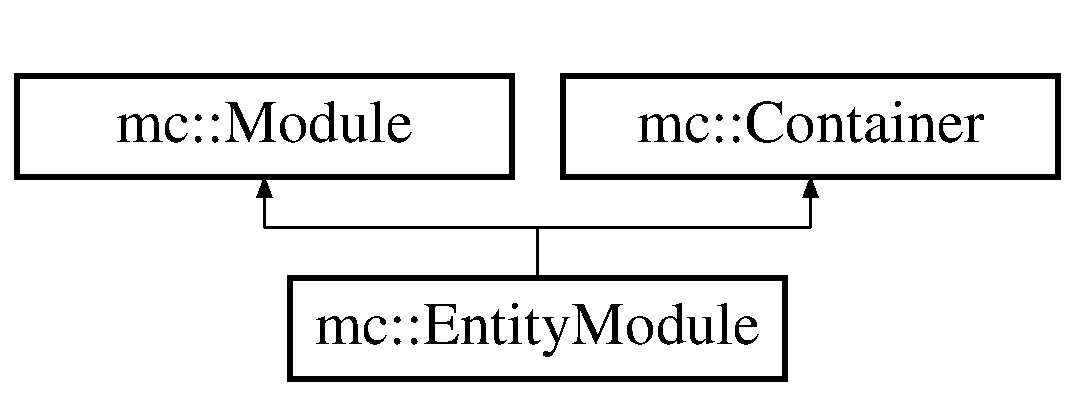
\includegraphics[height=2.000000cm]{dd/d2e/classmc_1_1_entity_module}
\end{center}
\end{figure}
\subsection*{Public Member Functions}
\begin{DoxyCompactItemize}
\item 
\hyperlink{classmc_1_1_entity_module_a38694a974571e19a231b4a62427259cf}{Entity\+Module} ()
\item 
void \hyperlink{classmc_1_1_entity_module_a5e1f25e0d12c50f6e8d8fbdf31028b8e}{init} ()
\begin{DoxyCompactList}\small\item\em Should be called every time \hyperlink{classmc_1_1_system_a86b7559895967af432c5c3db728bd0bc}{System\#init()} is called. \end{DoxyCompactList}\item 
void \hyperlink{classmc_1_1_entity_module_a3307eb2ce5af81b6a6e26fdaa12e3063}{update} ()
\begin{DoxyCompactList}\small\item\em Should be called every time \hyperlink{classmc_1_1_system_a90e14e44eb5a6019c913a6a197deb4a0}{System\#update()} is called. \end{DoxyCompactList}\item 
void \hyperlink{classmc_1_1_entity_module_a6c0fe0216850bb703df6721940f78b5f}{destroy} ()
\begin{DoxyCompactList}\small\item\em Should be called every time \hyperlink{}{System\#destroy()} is called. \end{DoxyCompactList}\item 
std\+::string \hyperlink{classmc_1_1_entity_module_aa943b1cfb590b01ce6f8a2d749a505bd}{get\+Name} () const 
\end{DoxyCompactItemize}
\subsection*{Additional Inherited Members}


\subsection{Constructor \& Destructor Documentation}
\index{mc\+::\+Entity\+Module@{mc\+::\+Entity\+Module}!Entity\+Module@{Entity\+Module}}
\index{Entity\+Module@{Entity\+Module}!mc\+::\+Entity\+Module@{mc\+::\+Entity\+Module}}
\subsubsection[{\texorpdfstring{Entity\+Module()}{EntityModule()}}]{\setlength{\rightskip}{0pt plus 5cm}mc\+::\+Entity\+Module\+::\+Entity\+Module (
\begin{DoxyParamCaption}
{}
\end{DoxyParamCaption}
)}\hypertarget{classmc_1_1_entity_module_a38694a974571e19a231b4a62427259cf}{}\label{classmc_1_1_entity_module_a38694a974571e19a231b4a62427259cf}


\subsection{Member Function Documentation}
\index{mc\+::\+Entity\+Module@{mc\+::\+Entity\+Module}!destroy@{destroy}}
\index{destroy@{destroy}!mc\+::\+Entity\+Module@{mc\+::\+Entity\+Module}}
\subsubsection[{\texorpdfstring{destroy()}{destroy()}}]{\setlength{\rightskip}{0pt plus 5cm}void mc\+::\+Entity\+Module\+::destroy (
\begin{DoxyParamCaption}
{}
\end{DoxyParamCaption}
)\hspace{0.3cm}{\ttfamily [virtual]}}\hypertarget{classmc_1_1_entity_module_a6c0fe0216850bb703df6721940f78b5f}{}\label{classmc_1_1_entity_module_a6c0fe0216850bb703df6721940f78b5f}


Should be called every time \hyperlink{}{System\#destroy()} is called. 

Calls
\begin{DoxyCode}
\hyperlink{classmc_1_1_entity_module_a6c0fe0216850bb703df6721940f78b5f}{destroy}() 
\end{DoxyCode}
 on all of this
\begin{DoxyCode}
Container\textcolor{stringliteral}{'s }
\end{DoxyCode}
 children. 

Reimplemented from \hyperlink{classmc_1_1_container_a80bd71e4e12ec218e4de88f4e48cc771}{mc\+::\+Container}.

\index{mc\+::\+Entity\+Module@{mc\+::\+Entity\+Module}!get\+Name@{get\+Name}}
\index{get\+Name@{get\+Name}!mc\+::\+Entity\+Module@{mc\+::\+Entity\+Module}}
\subsubsection[{\texorpdfstring{get\+Name() const }{getName() const }}]{\setlength{\rightskip}{0pt plus 5cm}std\+::string mc\+::\+Entity\+Module\+::get\+Name (
\begin{DoxyParamCaption}
{}
\end{DoxyParamCaption}
) const\hspace{0.3cm}{\ttfamily [virtual]}}\hypertarget{classmc_1_1_entity_module_aa943b1cfb590b01ce6f8a2d749a505bd}{}\label{classmc_1_1_entity_module_aa943b1cfb590b01ce6f8a2d749a505bd}


Implements \hyperlink{classmc_1_1_module_aa6d981a55ad5c04a39768e3ddcb0ad49}{mc\+::\+Module}.

\index{mc\+::\+Entity\+Module@{mc\+::\+Entity\+Module}!init@{init}}
\index{init@{init}!mc\+::\+Entity\+Module@{mc\+::\+Entity\+Module}}
\subsubsection[{\texorpdfstring{init()}{init()}}]{\setlength{\rightskip}{0pt plus 5cm}void mc\+::\+Entity\+Module\+::init (
\begin{DoxyParamCaption}
{}
\end{DoxyParamCaption}
)\hspace{0.3cm}{\ttfamily [virtual]}}\hypertarget{classmc_1_1_entity_module_a5e1f25e0d12c50f6e8d8fbdf31028b8e}{}\label{classmc_1_1_entity_module_a5e1f25e0d12c50f6e8d8fbdf31028b8e}


Should be called every time \hyperlink{classmc_1_1_system_a86b7559895967af432c5c3db728bd0bc}{System\#init()} is called. 

Calls
\begin{DoxyCode}
\hyperlink{classmc_1_1_entity_module_a5e1f25e0d12c50f6e8d8fbdf31028b8e}{init}() 
\end{DoxyCode}
 on all of this
\begin{DoxyCode}
Container\textcolor{stringliteral}{'s }
\end{DoxyCode}
 children. 

Reimplemented from \hyperlink{classmc_1_1_container_a087d26907d06163aa731d9a313163b7f}{mc\+::\+Container}.

\index{mc\+::\+Entity\+Module@{mc\+::\+Entity\+Module}!update@{update}}
\index{update@{update}!mc\+::\+Entity\+Module@{mc\+::\+Entity\+Module}}
\subsubsection[{\texorpdfstring{update()}{update()}}]{\setlength{\rightskip}{0pt plus 5cm}void mc\+::\+Entity\+Module\+::update (
\begin{DoxyParamCaption}
{}
\end{DoxyParamCaption}
)\hspace{0.3cm}{\ttfamily [virtual]}}\hypertarget{classmc_1_1_entity_module_a3307eb2ce5af81b6a6e26fdaa12e3063}{}\label{classmc_1_1_entity_module_a3307eb2ce5af81b6a6e26fdaa12e3063}


Should be called every time \hyperlink{classmc_1_1_system_a90e14e44eb5a6019c913a6a197deb4a0}{System\#update()} is called. 

Calls
\begin{DoxyCode}
\hyperlink{classmc_1_1_entity_module_a3307eb2ce5af81b6a6e26fdaa12e3063}{update}() 
\end{DoxyCode}
 on all of this
\begin{DoxyCode}
Container\textcolor{stringliteral}{'s }
\end{DoxyCode}
 children. 

Reimplemented from \hyperlink{classmc_1_1_container_a306bb7d15cee23ff8bef4b9342ed85cf}{mc\+::\+Container}.



The documentation for this class was generated from the following files\+:\begin{DoxyCompactItemize}
\item 
D\+:/\+Workspace/\+M\+A\+C\+E/\+M\+C-\/\+System/\+Entities/\hyperlink{_entity_8h}{Entity.\+h}\item 
D\+:/\+Workspace/\+M\+A\+C\+E/\+M\+C-\/\+System/\+Entities/\hyperlink{_entity_8cpp}{Entity.\+cpp}\end{DoxyCompactItemize}

\hypertarget{classmc_1_1_graphics_module}{}\section{mc\+:\+:Graphics\+Module Class Reference}
\label{classmc_1_1_graphics_module}\index{mc\+::\+Graphics\+Module@{mc\+::\+Graphics\+Module}}


{\ttfamily \#include $<$Graphics.\+h$>$}

Inheritance diagram for mc\+:\+:Graphics\+Module\+:\begin{figure}[H]
\begin{center}
\leavevmode
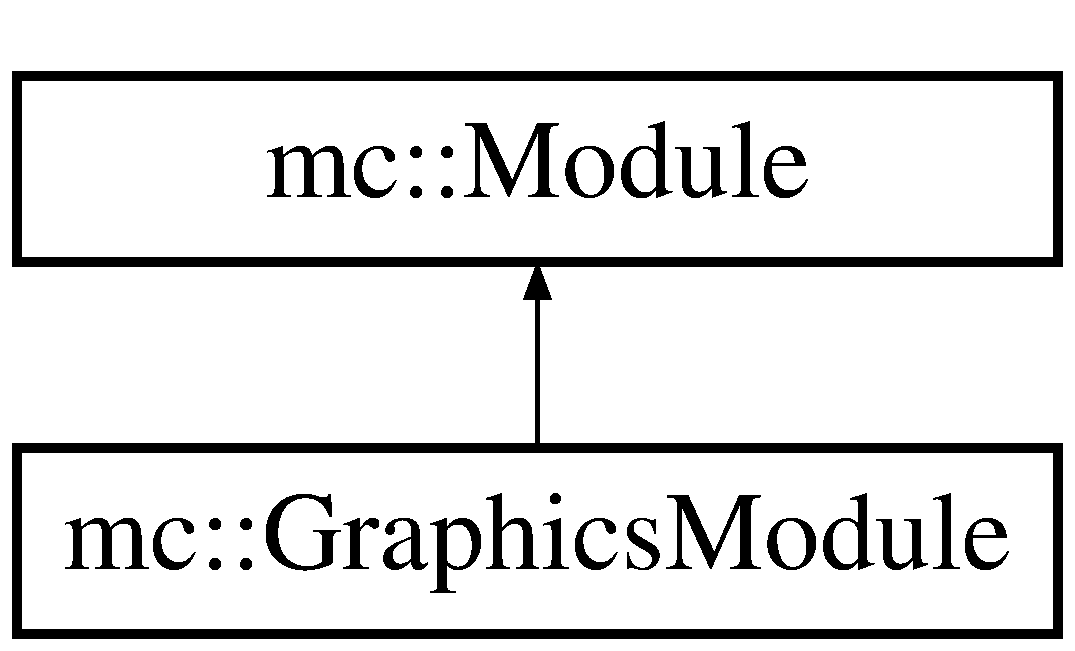
\includegraphics[height=2.000000cm]{classmc_1_1_graphics_module}
\end{center}
\end{figure}
\subsection*{Public Member Functions}
\begin{DoxyCompactItemize}
\item 
\hyperlink{_s_d_l__opengles2__gl2ext_8h_ae5d8fa23ad07c48bb609509eae494c95}{void} \hyperlink{classmc_1_1_graphics_module_aa25a958db86ea6930fb4c7d0d98dc1ab}{init} ()
\item 
\hyperlink{_s_d_l__opengles2__gl2ext_8h_ae5d8fa23ad07c48bb609509eae494c95}{void} \hyperlink{classmc_1_1_graphics_module_a80293bd6706490288419bb359ee544a6}{tick} ()
\item 
\hyperlink{_s_d_l__opengles2__gl2ext_8h_ae5d8fa23ad07c48bb609509eae494c95}{void} \hyperlink{classmc_1_1_graphics_module_af03308d7f2b29600d667077fa0370672}{destroy} ()
\item 
\hyperlink{_s_d_l__opengl__glext_8h_ae84541b4f3d8e1ea24ec0f466a8c568b}{std\+::string} \hyperlink{classmc_1_1_graphics_module_a3ff79450c20afe48690200d228fb380b}{get\+Name} () const 
\end{DoxyCompactItemize}
\subsection*{Additional Inherited Members}


\subsection{Member Function Documentation}
\index{mc\+::\+Graphics\+Module@{mc\+::\+Graphics\+Module}!destroy@{destroy}}
\index{destroy@{destroy}!mc\+::\+Graphics\+Module@{mc\+::\+Graphics\+Module}}
\subsubsection[{\texorpdfstring{destroy()}{destroy()}}]{\setlength{\rightskip}{0pt plus 5cm}{\bf void} mc\+::\+Graphics\+Module\+::destroy (
\begin{DoxyParamCaption}
{}
\end{DoxyParamCaption}
)\hspace{0.3cm}{\ttfamily [virtual]}}\hypertarget{classmc_1_1_graphics_module_af03308d7f2b29600d667077fa0370672}{}\label{classmc_1_1_graphics_module_af03308d7f2b29600d667077fa0370672}


Implements \hyperlink{classmc_1_1_module_abf13bd45de10185d4139dfff22a555d2}{mc\+::\+Module}.

\index{mc\+::\+Graphics\+Module@{mc\+::\+Graphics\+Module}!get\+Name@{get\+Name}}
\index{get\+Name@{get\+Name}!mc\+::\+Graphics\+Module@{mc\+::\+Graphics\+Module}}
\subsubsection[{\texorpdfstring{get\+Name() const }{getName() const }}]{\setlength{\rightskip}{0pt plus 5cm}{\bf std\+::string} mc\+::\+Graphics\+Module\+::get\+Name (
\begin{DoxyParamCaption}
{}
\end{DoxyParamCaption}
) const\hspace{0.3cm}{\ttfamily [virtual]}}\hypertarget{classmc_1_1_graphics_module_a3ff79450c20afe48690200d228fb380b}{}\label{classmc_1_1_graphics_module_a3ff79450c20afe48690200d228fb380b}


Implements \hyperlink{classmc_1_1_module_aa6d981a55ad5c04a39768e3ddcb0ad49}{mc\+::\+Module}.

\index{mc\+::\+Graphics\+Module@{mc\+::\+Graphics\+Module}!init@{init}}
\index{init@{init}!mc\+::\+Graphics\+Module@{mc\+::\+Graphics\+Module}}
\subsubsection[{\texorpdfstring{init()}{init()}}]{\setlength{\rightskip}{0pt plus 5cm}{\bf void} mc\+::\+Graphics\+Module\+::init (
\begin{DoxyParamCaption}
{}
\end{DoxyParamCaption}
)\hspace{0.3cm}{\ttfamily [virtual]}}\hypertarget{classmc_1_1_graphics_module_aa25a958db86ea6930fb4c7d0d98dc1ab}{}\label{classmc_1_1_graphics_module_aa25a958db86ea6930fb4c7d0d98dc1ab}


Implements \hyperlink{classmc_1_1_module_a854aad3bb8a2f60446fb14aeb28967b6}{mc\+::\+Module}.

\index{mc\+::\+Graphics\+Module@{mc\+::\+Graphics\+Module}!tick@{tick}}
\index{tick@{tick}!mc\+::\+Graphics\+Module@{mc\+::\+Graphics\+Module}}
\subsubsection[{\texorpdfstring{tick()}{tick()}}]{\setlength{\rightskip}{0pt plus 5cm}{\bf void} mc\+::\+Graphics\+Module\+::tick (
\begin{DoxyParamCaption}
{}
\end{DoxyParamCaption}
)}\hypertarget{classmc_1_1_graphics_module_a80293bd6706490288419bb359ee544a6}{}\label{classmc_1_1_graphics_module_a80293bd6706490288419bb359ee544a6}


The documentation for this class was generated from the following files\+:\begin{DoxyCompactItemize}
\item 
D\+:/\+Workspace/\+M\+A\+C\+E/\+M\+C-\/\+Graphics/\hyperlink{_graphics_8h}{Graphics.\+h}\item 
D\+:/\+Workspace/\+M\+A\+C\+E/\+M\+C-\/\+Graphics/\hyperlink{_graphics_8cpp}{Graphics.\+cpp}\end{DoxyCompactItemize}

\hypertarget{structmc_1_1_index_out_of_bounds}{}\section{mc\+:\+:Index\+Out\+Of\+Bounds Struct Reference}
\label{structmc_1_1_index_out_of_bounds}\index{mc\+::\+Index\+Out\+Of\+Bounds@{mc\+::\+Index\+Out\+Of\+Bounds}}


{\ttfamily \#include $<$Exceptions.\+h$>$}

Inheritance diagram for mc\+:\+:Index\+Out\+Of\+Bounds\+:\begin{figure}[H]
\begin{center}
\leavevmode
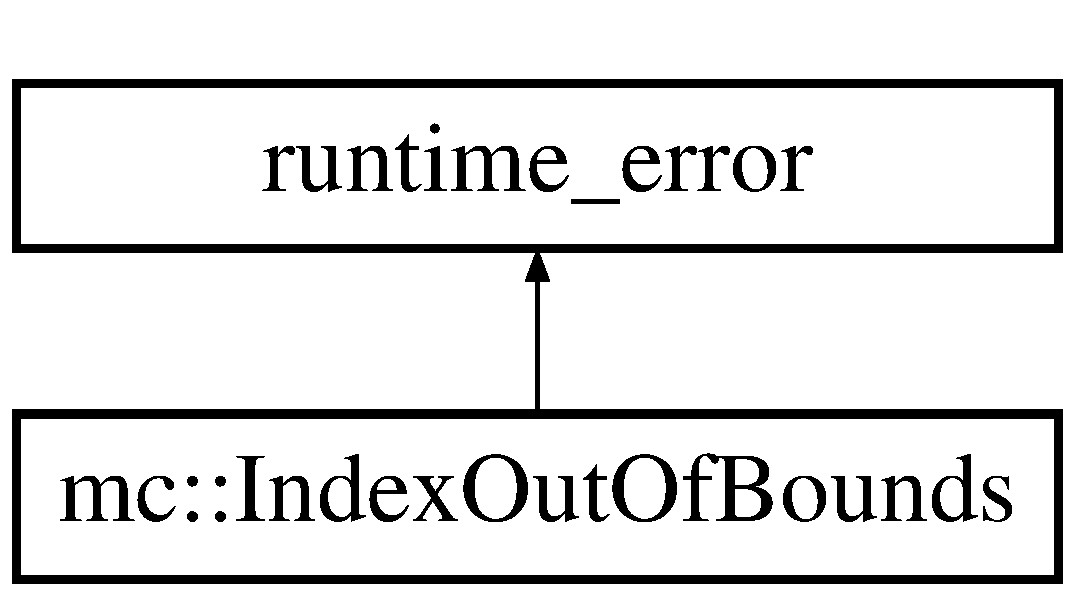
\includegraphics[height=2.000000cm]{structmc_1_1_index_out_of_bounds}
\end{center}
\end{figure}
\subsection*{Public Member Functions}
\begin{DoxyCompactItemize}
\item 
\hyperlink{structmc_1_1_index_out_of_bounds_aa4f02ccacfffa4f3470b4b4c7faf7ebd}{Index\+Out\+Of\+Bounds} (const char $\ast$\hyperlink{_s_d_l__opengl__glext_8h_a1f2d7f8147412c43ba2303a56f97ee73}{c}=\char`\"{}No \hyperlink{_s_d_l__opengl__glext_8h_a7b6161cffb9b8aee272b3b916183d28c}{message} was given\char`\"{})
\item 
\hyperlink{structmc_1_1_index_out_of_bounds_a52360d4332f55b0757bcf25668970eff}{Index\+Out\+Of\+Bounds} (const \hyperlink{_s_d_l__opengl__glext_8h_ae84541b4f3d8e1ea24ec0f466a8c568b}{std\+::string} \hyperlink{_s_d_l__opengl__glext_8h_a1f2d7f8147412c43ba2303a56f97ee73}{c}=\char`\"{}No \hyperlink{_s_d_l__opengl__glext_8h_a7b6161cffb9b8aee272b3b916183d28c}{message} was given\char`\"{})
\end{DoxyCompactItemize}


\subsection{Constructor \& Destructor Documentation}
\index{mc\+::\+Index\+Out\+Of\+Bounds@{mc\+::\+Index\+Out\+Of\+Bounds}!Index\+Out\+Of\+Bounds@{Index\+Out\+Of\+Bounds}}
\index{Index\+Out\+Of\+Bounds@{Index\+Out\+Of\+Bounds}!mc\+::\+Index\+Out\+Of\+Bounds@{mc\+::\+Index\+Out\+Of\+Bounds}}
\subsubsection[{\texorpdfstring{Index\+Out\+Of\+Bounds(const char $\ast$c=""No message was given"")}{IndexOutOfBounds(const char *c="No message was given")}}]{\setlength{\rightskip}{0pt plus 5cm}mc\+::\+Index\+Out\+Of\+Bounds\+::\+Index\+Out\+Of\+Bounds (
\begin{DoxyParamCaption}
\item[{const char $\ast$}]{c = {\ttfamily \char`\"{}No~{\bf message}~was~given\char`\"{}}}
\end{DoxyParamCaption}
)\hspace{0.3cm}{\ttfamily [inline]}, {\ttfamily [explicit]}}\hypertarget{structmc_1_1_index_out_of_bounds_aa4f02ccacfffa4f3470b4b4c7faf7ebd}{}\label{structmc_1_1_index_out_of_bounds_aa4f02ccacfffa4f3470b4b4c7faf7ebd}
\index{mc\+::\+Index\+Out\+Of\+Bounds@{mc\+::\+Index\+Out\+Of\+Bounds}!Index\+Out\+Of\+Bounds@{Index\+Out\+Of\+Bounds}}
\index{Index\+Out\+Of\+Bounds@{Index\+Out\+Of\+Bounds}!mc\+::\+Index\+Out\+Of\+Bounds@{mc\+::\+Index\+Out\+Of\+Bounds}}
\subsubsection[{\texorpdfstring{Index\+Out\+Of\+Bounds(const std\+::string c=""No message was given"")}{IndexOutOfBounds(const std::string c="No message was given")}}]{\setlength{\rightskip}{0pt plus 5cm}mc\+::\+Index\+Out\+Of\+Bounds\+::\+Index\+Out\+Of\+Bounds (
\begin{DoxyParamCaption}
\item[{const {\bf std\+::string}}]{c = {\ttfamily \char`\"{}No~{\bf message}~was~given\char`\"{}}}
\end{DoxyParamCaption}
)\hspace{0.3cm}{\ttfamily [inline]}, {\ttfamily [explicit]}}\hypertarget{structmc_1_1_index_out_of_bounds_a52360d4332f55b0757bcf25668970eff}{}\label{structmc_1_1_index_out_of_bounds_a52360d4332f55b0757bcf25668970eff}


The documentation for this struct was generated from the following file\+:\begin{DoxyCompactItemize}
\item 
D\+:/\+Workspace/\+M\+A\+C\+E/\+M\+C-\/\+System/\hyperlink{_exceptions_8h}{Exceptions.\+h}\end{DoxyCompactItemize}

\hypertarget{classmc_1_1_math}{}\section{mc\+:\+:Math Class Reference}
\label{classmc_1_1_math}\index{mc\+::\+Math@{mc\+::\+Math}}


{\ttfamily \#include $<$Math.\+h$>$}

\subsection*{Static Public Member Functions}
\begin{DoxyCompactItemize}
\item 
static int \hyperlink{classmc_1_1_math_a761878b5c3df8f3c0a8fdd24fa76b371}{floor} (double value)
\item 
static bool \hyperlink{classmc_1_1_math_a8259956dd9b5fbd727125205c8c992ba}{is\+Prime} (int value)
\item 
static double \hyperlink{classmc_1_1_math_a07106fd3a808226b1ada3a5064296da2}{tan} (double radians)
\item 
static double \hyperlink{classmc_1_1_math_aabae3b51035367461fc3e0b1c528d56d}{to\+Radians} (double degrees)
\item 
static int \hyperlink{classmc_1_1_math_a1c1ff42463d211c0714ff390a9a34db3}{next\+Digit\+Of2} (int n)
\item 
static \hyperlink{namespacemc_afd32b9ea49ccd962bb337dc71450595b}{Matrix4f} \hyperlink{classmc_1_1_math_a399c5c15df979f3f0c38464fc2e12306}{get\+Projection\+Matrix} (float F\+OV, float N\+E\+A\+R\+\_\+\+P\+L\+A\+NE, float F\+A\+R\+\_\+\+P\+L\+A\+NE, float aspect\+Ratio)
\end{DoxyCompactItemize}


\subsection{Member Function Documentation}
\index{mc\+::\+Math@{mc\+::\+Math}!floor@{floor}}
\index{floor@{floor}!mc\+::\+Math@{mc\+::\+Math}}
\subsubsection[{\texorpdfstring{floor(double value)}{floor(double value)}}]{\setlength{\rightskip}{0pt plus 5cm}int mc\+::\+Math\+::floor (
\begin{DoxyParamCaption}
\item[{double}]{value}
\end{DoxyParamCaption}
)\hspace{0.3cm}{\ttfamily [static]}}\hypertarget{classmc_1_1_math_a761878b5c3df8f3c0a8fdd24fa76b371}{}\label{classmc_1_1_math_a761878b5c3df8f3c0a8fdd24fa76b371}
\index{mc\+::\+Math@{mc\+::\+Math}!get\+Projection\+Matrix@{get\+Projection\+Matrix}}
\index{get\+Projection\+Matrix@{get\+Projection\+Matrix}!mc\+::\+Math@{mc\+::\+Math}}
\subsubsection[{\texorpdfstring{get\+Projection\+Matrix(float F\+O\+V, float N\+E\+A\+R\+\_\+\+P\+L\+A\+N\+E, float F\+A\+R\+\_\+\+P\+L\+A\+N\+E, float aspect\+Ratio)}{getProjectionMatrix(float FOV, float NEAR_PLANE, float FAR_PLANE, float aspectRatio)}}]{\setlength{\rightskip}{0pt plus 5cm}static {\bf Matrix4f} mc\+::\+Math\+::get\+Projection\+Matrix (
\begin{DoxyParamCaption}
\item[{float}]{F\+OV, }
\item[{float}]{N\+E\+A\+R\+\_\+\+P\+L\+A\+NE, }
\item[{float}]{F\+A\+R\+\_\+\+P\+L\+A\+NE, }
\item[{float}]{aspect\+Ratio}
\end{DoxyParamCaption}
)\hspace{0.3cm}{\ttfamily [static]}}\hypertarget{classmc_1_1_math_a399c5c15df979f3f0c38464fc2e12306}{}\label{classmc_1_1_math_a399c5c15df979f3f0c38464fc2e12306}
\index{mc\+::\+Math@{mc\+::\+Math}!is\+Prime@{is\+Prime}}
\index{is\+Prime@{is\+Prime}!mc\+::\+Math@{mc\+::\+Math}}
\subsubsection[{\texorpdfstring{is\+Prime(int value)}{isPrime(int value)}}]{\setlength{\rightskip}{0pt plus 5cm}bool mc\+::\+Math\+::is\+Prime (
\begin{DoxyParamCaption}
\item[{int}]{value}
\end{DoxyParamCaption}
)\hspace{0.3cm}{\ttfamily [static]}}\hypertarget{classmc_1_1_math_a8259956dd9b5fbd727125205c8c992ba}{}\label{classmc_1_1_math_a8259956dd9b5fbd727125205c8c992ba}
\index{mc\+::\+Math@{mc\+::\+Math}!next\+Digit\+Of2@{next\+Digit\+Of2}}
\index{next\+Digit\+Of2@{next\+Digit\+Of2}!mc\+::\+Math@{mc\+::\+Math}}
\subsubsection[{\texorpdfstring{next\+Digit\+Of2(int n)}{nextDigitOf2(int n)}}]{\setlength{\rightskip}{0pt plus 5cm}int mc\+::\+Math\+::next\+Digit\+Of2 (
\begin{DoxyParamCaption}
\item[{int}]{n}
\end{DoxyParamCaption}
)\hspace{0.3cm}{\ttfamily [static]}}\hypertarget{classmc_1_1_math_a1c1ff42463d211c0714ff390a9a34db3}{}\label{classmc_1_1_math_a1c1ff42463d211c0714ff390a9a34db3}
\index{mc\+::\+Math@{mc\+::\+Math}!tan@{tan}}
\index{tan@{tan}!mc\+::\+Math@{mc\+::\+Math}}
\subsubsection[{\texorpdfstring{tan(double radians)}{tan(double radians)}}]{\setlength{\rightskip}{0pt plus 5cm}static double mc\+::\+Math\+::tan (
\begin{DoxyParamCaption}
\item[{double}]{radians}
\end{DoxyParamCaption}
)\hspace{0.3cm}{\ttfamily [static]}}\hypertarget{classmc_1_1_math_a07106fd3a808226b1ada3a5064296da2}{}\label{classmc_1_1_math_a07106fd3a808226b1ada3a5064296da2}
\index{mc\+::\+Math@{mc\+::\+Math}!to\+Radians@{to\+Radians}}
\index{to\+Radians@{to\+Radians}!mc\+::\+Math@{mc\+::\+Math}}
\subsubsection[{\texorpdfstring{to\+Radians(double degrees)}{toRadians(double degrees)}}]{\setlength{\rightskip}{0pt plus 5cm}static double mc\+::\+Math\+::to\+Radians (
\begin{DoxyParamCaption}
\item[{double}]{degrees}
\end{DoxyParamCaption}
)\hspace{0.3cm}{\ttfamily [static]}}\hypertarget{classmc_1_1_math_aabae3b51035367461fc3e0b1c528d56d}{}\label{classmc_1_1_math_aabae3b51035367461fc3e0b1c528d56d}


The documentation for this class was generated from the following files\+:\begin{DoxyCompactItemize}
\item 
D\+:/\+Workspace/\+M\+A\+C\+E/\+M\+C-\/\+System/\+Utility/\hyperlink{_math_8h}{Math.\+h}\item 
D\+:/\+Workspace/\+M\+A\+C\+E/\+M\+C-\/\+System/\+Utility/\hyperlink{_math_8cpp}{Math.\+cpp}\end{DoxyCompactItemize}

\hypertarget{structmc_1_1_matrix}{}\section{mc\+:\+:Matrix$<$ T, W, H $>$ Struct Template Reference}
\label{structmc_1_1_matrix}\index{mc\+::\+Matrix$<$ T, W, H $>$@{mc\+::\+Matrix$<$ T, W, H $>$}}


{\ttfamily \#include $<$Vector.\+h$>$}

Inheritance diagram for mc\+:\+:Matrix$<$ T, W, H $>$\+:\begin{figure}[H]
\begin{center}
\leavevmode
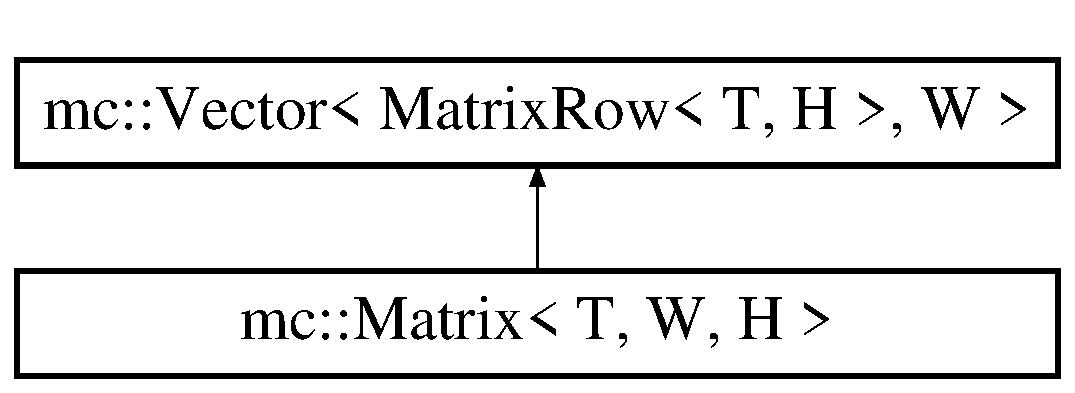
\includegraphics[height=2.000000cm]{structmc_1_1_matrix}
\end{center}
\end{figure}
\subsection*{Public Member Functions}
\begin{DoxyCompactItemize}
\item 
\hyperlink{structmc_1_1_matrix_a1c0107dd6bf262a240653fcc2650fb2b}{Matrix} ()
\item 
\hyperlink{structmc_1_1_matrix_a4bceda87f2c87294d4a631b2229dff8f}{Matrix} (T arr\mbox{[}W\mbox{]}\mbox{[}H\mbox{]})
\item 
\hyperlink{structmc_1_1_matrix_a16a62a958729f121805a76d43554bc69}{Matrix} (const \hyperlink{structmc_1_1_matrix}{Matrix} \&copy)
\item 
\hyperlink{namespacemc_ad1c06461067735b3b17e0df612532c4e}{Size} \hyperlink{structmc_1_1_matrix_ac7b493824ba976376aeac2de193f41f2}{size} ()
\item 
\hyperlink{namespacemc_ad1c06461067735b3b17e0df612532c4e}{Size} \hyperlink{structmc_1_1_matrix_af50d7f0d342318246a98fb7e01ae4989}{width} ()
\item 
\hyperlink{namespacemc_ad1c06461067735b3b17e0df612532c4e}{Size} \hyperlink{structmc_1_1_matrix_ad9eaa721ec2db5bb588ae12e6c2a78b3}{height} ()
\item 
T \& \hyperlink{structmc_1_1_matrix_ad4c47d5e7ef5c88264b06554a64f7ae7}{get} (unsigned \hyperlink{_s_d_l__thread_8h_a6a64f9be4433e4de6e2f2f548cf3c08e}{int} \hyperlink{_s_d_l__opengl_8h_ad0e63d0edcdbd3d79554076bf309fd47}{x}, unsigned \hyperlink{_s_d_l__thread_8h_a6a64f9be4433e4de6e2f2f548cf3c08e}{int} \hyperlink{_s_d_l__opengl_8h_a1675d9d7bb68e1657ff028643b4037e3}{y})
\item 
const T \& \hyperlink{structmc_1_1_matrix_aa8cca780babd0f83797e05400538ad69}{get} (unsigned \hyperlink{_s_d_l__thread_8h_a6a64f9be4433e4de6e2f2f548cf3c08e}{int} \hyperlink{_s_d_l__opengl_8h_ad0e63d0edcdbd3d79554076bf309fd47}{x}, unsigned \hyperlink{_s_d_l__thread_8h_a6a64f9be4433e4de6e2f2f548cf3c08e}{int} \hyperlink{_s_d_l__opengl_8h_a1675d9d7bb68e1657ff028643b4037e3}{y}) const 
\item 
\hyperlink{_s_d_l__opengles2__gl2ext_8h_ae5d8fa23ad07c48bb609509eae494c95}{void} \hyperlink{structmc_1_1_matrix_a7a4970e6c6d4c277cd7d15cffb3e470f}{set} (unsigned \hyperlink{_s_d_l__thread_8h_a6a64f9be4433e4de6e2f2f548cf3c08e}{int} \hyperlink{_s_d_l__opengl_8h_ad0e63d0edcdbd3d79554076bf309fd47}{x}, unsigned \hyperlink{_s_d_l__thread_8h_a6a64f9be4433e4de6e2f2f548cf3c08e}{int} \hyperlink{_s_d_l__opengl_8h_a1675d9d7bb68e1657ff028643b4037e3}{y}, T \hyperlink{_s_d_l__opengl__glext_8h_a8ad81492d410ff2ac11f754f4042150f}{value})
\end{DoxyCompactItemize}
\subsection*{Additional Inherited Members}


\subsection{Constructor \& Destructor Documentation}
\index{mc\+::\+Matrix@{mc\+::\+Matrix}!Matrix@{Matrix}}
\index{Matrix@{Matrix}!mc\+::\+Matrix@{mc\+::\+Matrix}}
\subsubsection[{\texorpdfstring{Matrix()}{Matrix()}}]{\setlength{\rightskip}{0pt plus 5cm}template$<$typename T , int W, int H$>$ {\bf mc\+::\+Matrix}$<$ T, W, H $>$\+::{\bf Matrix} (
\begin{DoxyParamCaption}
{}
\end{DoxyParamCaption}
)\hspace{0.3cm}{\ttfamily [inline]}}\hypertarget{structmc_1_1_matrix_a1c0107dd6bf262a240653fcc2650fb2b}{}\label{structmc_1_1_matrix_a1c0107dd6bf262a240653fcc2650fb2b}
\index{mc\+::\+Matrix@{mc\+::\+Matrix}!Matrix@{Matrix}}
\index{Matrix@{Matrix}!mc\+::\+Matrix@{mc\+::\+Matrix}}
\subsubsection[{\texorpdfstring{Matrix(\+T arr[W][H])}{Matrix(T arr[W][H])}}]{\setlength{\rightskip}{0pt plus 5cm}template$<$typename T , int W, int H$>$ {\bf mc\+::\+Matrix}$<$ T, W, H $>$\+::{\bf Matrix} (
\begin{DoxyParamCaption}
\item[{T}]{arr\mbox{[}\+W\mbox{]}\mbox{[}\+H\mbox{]}}
\end{DoxyParamCaption}
)\hspace{0.3cm}{\ttfamily [inline]}}\hypertarget{structmc_1_1_matrix_a4bceda87f2c87294d4a631b2229dff8f}{}\label{structmc_1_1_matrix_a4bceda87f2c87294d4a631b2229dff8f}
\index{mc\+::\+Matrix@{mc\+::\+Matrix}!Matrix@{Matrix}}
\index{Matrix@{Matrix}!mc\+::\+Matrix@{mc\+::\+Matrix}}
\subsubsection[{\texorpdfstring{Matrix(const Matrix \&copy)}{Matrix(const Matrix &copy)}}]{\setlength{\rightskip}{0pt plus 5cm}template$<$typename T , int W, int H$>$ {\bf mc\+::\+Matrix}$<$ T, W, H $>$\+::{\bf Matrix} (
\begin{DoxyParamCaption}
\item[{const {\bf Matrix}$<$ T, W, H $>$ \&}]{copy}
\end{DoxyParamCaption}
)\hspace{0.3cm}{\ttfamily [inline]}}\hypertarget{structmc_1_1_matrix_a16a62a958729f121805a76d43554bc69}{}\label{structmc_1_1_matrix_a16a62a958729f121805a76d43554bc69}


\subsection{Member Function Documentation}
\index{mc\+::\+Matrix@{mc\+::\+Matrix}!get@{get}}
\index{get@{get}!mc\+::\+Matrix@{mc\+::\+Matrix}}
\subsubsection[{\texorpdfstring{get(unsigned int x, unsigned int y)}{get(unsigned int x, unsigned int y)}}]{\setlength{\rightskip}{0pt plus 5cm}template$<$typename T , int W, int H$>$ T\& {\bf mc\+::\+Matrix}$<$ T, W, H $>$\+::get (
\begin{DoxyParamCaption}
\item[{unsigned {\bf int}}]{x, }
\item[{unsigned {\bf int}}]{y}
\end{DoxyParamCaption}
)\hspace{0.3cm}{\ttfamily [inline]}}\hypertarget{structmc_1_1_matrix_ad4c47d5e7ef5c88264b06554a64f7ae7}{}\label{structmc_1_1_matrix_ad4c47d5e7ef5c88264b06554a64f7ae7}
\index{mc\+::\+Matrix@{mc\+::\+Matrix}!get@{get}}
\index{get@{get}!mc\+::\+Matrix@{mc\+::\+Matrix}}
\subsubsection[{\texorpdfstring{get(unsigned int x, unsigned int y) const }{get(unsigned int x, unsigned int y) const }}]{\setlength{\rightskip}{0pt plus 5cm}template$<$typename T , int W, int H$>$ const T\& {\bf mc\+::\+Matrix}$<$ T, W, H $>$\+::get (
\begin{DoxyParamCaption}
\item[{unsigned {\bf int}}]{x, }
\item[{unsigned {\bf int}}]{y}
\end{DoxyParamCaption}
) const\hspace{0.3cm}{\ttfamily [inline]}}\hypertarget{structmc_1_1_matrix_aa8cca780babd0f83797e05400538ad69}{}\label{structmc_1_1_matrix_aa8cca780babd0f83797e05400538ad69}
\index{mc\+::\+Matrix@{mc\+::\+Matrix}!height@{height}}
\index{height@{height}!mc\+::\+Matrix@{mc\+::\+Matrix}}
\subsubsection[{\texorpdfstring{height()}{height()}}]{\setlength{\rightskip}{0pt plus 5cm}template$<$typename T , int W, int H$>$ {\bf Size} {\bf mc\+::\+Matrix}$<$ T, W, H $>$\+::{\bf height} (
\begin{DoxyParamCaption}
{}
\end{DoxyParamCaption}
)\hspace{0.3cm}{\ttfamily [inline]}}\hypertarget{structmc_1_1_matrix_ad9eaa721ec2db5bb588ae12e6c2a78b3}{}\label{structmc_1_1_matrix_ad9eaa721ec2db5bb588ae12e6c2a78b3}
\index{mc\+::\+Matrix@{mc\+::\+Matrix}!set@{set}}
\index{set@{set}!mc\+::\+Matrix@{mc\+::\+Matrix}}
\subsubsection[{\texorpdfstring{set(unsigned int x, unsigned int y, T value)}{set(unsigned int x, unsigned int y, T value)}}]{\setlength{\rightskip}{0pt plus 5cm}template$<$typename T , int W, int H$>$ {\bf void} {\bf mc\+::\+Matrix}$<$ T, W, H $>$\+::set (
\begin{DoxyParamCaption}
\item[{unsigned {\bf int}}]{x, }
\item[{unsigned {\bf int}}]{y, }
\item[{T}]{value}
\end{DoxyParamCaption}
)\hspace{0.3cm}{\ttfamily [inline]}}\hypertarget{structmc_1_1_matrix_a7a4970e6c6d4c277cd7d15cffb3e470f}{}\label{structmc_1_1_matrix_a7a4970e6c6d4c277cd7d15cffb3e470f}
\index{mc\+::\+Matrix@{mc\+::\+Matrix}!size@{size}}
\index{size@{size}!mc\+::\+Matrix@{mc\+::\+Matrix}}
\subsubsection[{\texorpdfstring{size()}{size()}}]{\setlength{\rightskip}{0pt plus 5cm}template$<$typename T , int W, int H$>$ {\bf Size} {\bf mc\+::\+Matrix}$<$ T, W, H $>$\+::{\bf size} (
\begin{DoxyParamCaption}
{}
\end{DoxyParamCaption}
)\hspace{0.3cm}{\ttfamily [inline]}}\hypertarget{structmc_1_1_matrix_ac7b493824ba976376aeac2de193f41f2}{}\label{structmc_1_1_matrix_ac7b493824ba976376aeac2de193f41f2}
\index{mc\+::\+Matrix@{mc\+::\+Matrix}!width@{width}}
\index{width@{width}!mc\+::\+Matrix@{mc\+::\+Matrix}}
\subsubsection[{\texorpdfstring{width()}{width()}}]{\setlength{\rightskip}{0pt plus 5cm}template$<$typename T , int W, int H$>$ {\bf Size} {\bf mc\+::\+Matrix}$<$ T, W, H $>$\+::{\bf width} (
\begin{DoxyParamCaption}
{}
\end{DoxyParamCaption}
)\hspace{0.3cm}{\ttfamily [inline]}}\hypertarget{structmc_1_1_matrix_af50d7f0d342318246a98fb7e01ae4989}{}\label{structmc_1_1_matrix_af50d7f0d342318246a98fb7e01ae4989}


The documentation for this struct was generated from the following file\+:\begin{DoxyCompactItemize}
\item 
D\+:/\+Workspace/\+M\+A\+C\+E/\+M\+C-\/\+System/\+Utility/\hyperlink{_vector_8h}{Vector.\+h}\end{DoxyCompactItemize}

\hypertarget{classmc_1_1_module}{}\section{mc\+:\+:Module Class Reference}
\label{classmc_1_1_module}\index{mc\+::\+Module@{mc\+::\+Module}}


{\ttfamily \#include $<$System.\+h$>$}

Inheritance diagram for mc\+:\+:Module\+:\begin{figure}[H]
\begin{center}
\leavevmode
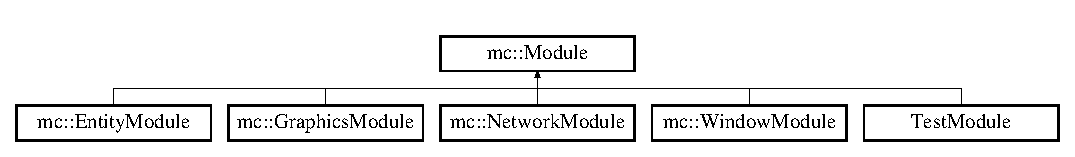
\includegraphics[height=1.659259cm]{classmc_1_1_module}
\end{center}
\end{figure}
\subsection*{Protected Member Functions}
\begin{DoxyCompactItemize}
\item 
virtual \hyperlink{_s_d_l__opengles2__gl2ext_8h_ae5d8fa23ad07c48bb609509eae494c95}{void} \hyperlink{classmc_1_1_module_a854aad3bb8a2f60446fb14aeb28967b6}{init} ()=0
\item 
virtual \hyperlink{_s_d_l__opengles2__gl2ext_8h_ae5d8fa23ad07c48bb609509eae494c95}{void} \hyperlink{classmc_1_1_module_a6417f3db90ae235fb1be01ed6a3d612c}{update} ()=0
\item 
virtual \hyperlink{_s_d_l__opengles2__gl2ext_8h_ae5d8fa23ad07c48bb609509eae494c95}{void} \hyperlink{classmc_1_1_module_abf13bd45de10185d4139dfff22a555d2}{destroy} ()=0
\item 
virtual \hyperlink{_s_d_l__opengl__glext_8h_ae84541b4f3d8e1ea24ec0f466a8c568b}{std\+::string} \hyperlink{classmc_1_1_module_aa6d981a55ad5c04a39768e3ddcb0ad49}{get\+Name} () const  =0
\end{DoxyCompactItemize}
\subsection*{Friends}
\begin{DoxyCompactItemize}
\item 
class \hyperlink{classmc_1_1_module_af18a9ee98e70982bfe2975391d7221a5}{System}
\end{DoxyCompactItemize}


\subsection{Member Function Documentation}
\index{mc\+::\+Module@{mc\+::\+Module}!destroy@{destroy}}
\index{destroy@{destroy}!mc\+::\+Module@{mc\+::\+Module}}
\subsubsection[{\texorpdfstring{destroy()=0}{destroy()=0}}]{\setlength{\rightskip}{0pt plus 5cm}virtual {\bf void} mc\+::\+Module\+::destroy (
\begin{DoxyParamCaption}
{}
\end{DoxyParamCaption}
)\hspace{0.3cm}{\ttfamily [protected]}, {\ttfamily [pure virtual]}}\hypertarget{classmc_1_1_module_abf13bd45de10185d4139dfff22a555d2}{}\label{classmc_1_1_module_abf13bd45de10185d4139dfff22a555d2}


Implemented in \hyperlink{classmc_1_1_entity_module_a6c0fe0216850bb703df6721940f78b5f}{mc\+::\+Entity\+Module}, \hyperlink{class_test_module_a58609817f503e9ca6e4fbb13282bb19a}{Test\+Module}, \hyperlink{classmc_1_1_window_module_a4ad68d037b1ed9aa8740d01a0c2f3762}{mc\+::\+Window\+Module}, \hyperlink{classmc_1_1_graphics_module_af03308d7f2b29600d667077fa0370672}{mc\+::\+Graphics\+Module}, and \hyperlink{classmc_1_1_network_module_a9cbb7fce204c10620ba2ba07f8f4a3a2}{mc\+::\+Network\+Module}.

\index{mc\+::\+Module@{mc\+::\+Module}!get\+Name@{get\+Name}}
\index{get\+Name@{get\+Name}!mc\+::\+Module@{mc\+::\+Module}}
\subsubsection[{\texorpdfstring{get\+Name() const  =0}{getName() const  =0}}]{\setlength{\rightskip}{0pt plus 5cm}virtual {\bf std\+::string} mc\+::\+Module\+::get\+Name (
\begin{DoxyParamCaption}
{}
\end{DoxyParamCaption}
) const\hspace{0.3cm}{\ttfamily [protected]}, {\ttfamily [pure virtual]}}\hypertarget{classmc_1_1_module_aa6d981a55ad5c04a39768e3ddcb0ad49}{}\label{classmc_1_1_module_aa6d981a55ad5c04a39768e3ddcb0ad49}


Implemented in \hyperlink{classmc_1_1_entity_module_aa943b1cfb590b01ce6f8a2d749a505bd}{mc\+::\+Entity\+Module}, \hyperlink{class_test_module_a1786c36358b0efcb5175a237cf331a5f}{Test\+Module}, \hyperlink{classmc_1_1_window_module_a69600ab76f3427c509594916abde0d37}{mc\+::\+Window\+Module}, \hyperlink{classmc_1_1_graphics_module_a3ff79450c20afe48690200d228fb380b}{mc\+::\+Graphics\+Module}, and \hyperlink{classmc_1_1_network_module_acf87542f4ba61dfe44c394da01ba8f4c}{mc\+::\+Network\+Module}.

\index{mc\+::\+Module@{mc\+::\+Module}!init@{init}}
\index{init@{init}!mc\+::\+Module@{mc\+::\+Module}}
\subsubsection[{\texorpdfstring{init()=0}{init()=0}}]{\setlength{\rightskip}{0pt plus 5cm}virtual {\bf void} mc\+::\+Module\+::init (
\begin{DoxyParamCaption}
{}
\end{DoxyParamCaption}
)\hspace{0.3cm}{\ttfamily [protected]}, {\ttfamily [pure virtual]}}\hypertarget{classmc_1_1_module_a854aad3bb8a2f60446fb14aeb28967b6}{}\label{classmc_1_1_module_a854aad3bb8a2f60446fb14aeb28967b6}


Implemented in \hyperlink{classmc_1_1_entity_module_a5e1f25e0d12c50f6e8d8fbdf31028b8e}{mc\+::\+Entity\+Module}, \hyperlink{class_test_module_a06a3a2e4ff5b7890ed209f56472108a6}{Test\+Module}, \hyperlink{classmc_1_1_window_module_acdc406a66ee7ab44277953b8429642ca}{mc\+::\+Window\+Module}, \hyperlink{classmc_1_1_graphics_module_aa25a958db86ea6930fb4c7d0d98dc1ab}{mc\+::\+Graphics\+Module}, and \hyperlink{classmc_1_1_network_module_ad5ec63cfdd43e8c4374dbbb65cfba3ff}{mc\+::\+Network\+Module}.

\index{mc\+::\+Module@{mc\+::\+Module}!update@{update}}
\index{update@{update}!mc\+::\+Module@{mc\+::\+Module}}
\subsubsection[{\texorpdfstring{update()=0}{update()=0}}]{\setlength{\rightskip}{0pt plus 5cm}virtual {\bf void} mc\+::\+Module\+::update (
\begin{DoxyParamCaption}
{}
\end{DoxyParamCaption}
)\hspace{0.3cm}{\ttfamily [protected]}, {\ttfamily [pure virtual]}}\hypertarget{classmc_1_1_module_a6417f3db90ae235fb1be01ed6a3d612c}{}\label{classmc_1_1_module_a6417f3db90ae235fb1be01ed6a3d612c}


Implemented in \hyperlink{classmc_1_1_entity_module_a3307eb2ce5af81b6a6e26fdaa12e3063}{mc\+::\+Entity\+Module}, and \hyperlink{class_test_module_a190147fb3851743518bc0e5773e4af3e}{Test\+Module}.



\subsection{Friends And Related Function Documentation}
\index{mc\+::\+Module@{mc\+::\+Module}!System@{System}}
\index{System@{System}!mc\+::\+Module@{mc\+::\+Module}}
\subsubsection[{\texorpdfstring{System}{System}}]{\setlength{\rightskip}{0pt plus 5cm}friend class {\bf System}\hspace{0.3cm}{\ttfamily [friend]}}\hypertarget{classmc_1_1_module_af18a9ee98e70982bfe2975391d7221a5}{}\label{classmc_1_1_module_af18a9ee98e70982bfe2975391d7221a5}


The documentation for this class was generated from the following file\+:\begin{DoxyCompactItemize}
\item 
D\+:/\+Workspace/\+M\+A\+C\+E/\+M\+C-\/\+System/\hyperlink{_system_8h}{System.\+h}\end{DoxyCompactItemize}

\hypertarget{classmc_1_1_network_module}{}\section{mc\+:\+:Network\+Module Class Reference}
\label{classmc_1_1_network_module}\index{mc\+::\+Network\+Module@{mc\+::\+Network\+Module}}


{\ttfamily \#include $<$Network.\+h$>$}

Inheritance diagram for mc\+:\+:Network\+Module\+:\begin{figure}[H]
\begin{center}
\leavevmode
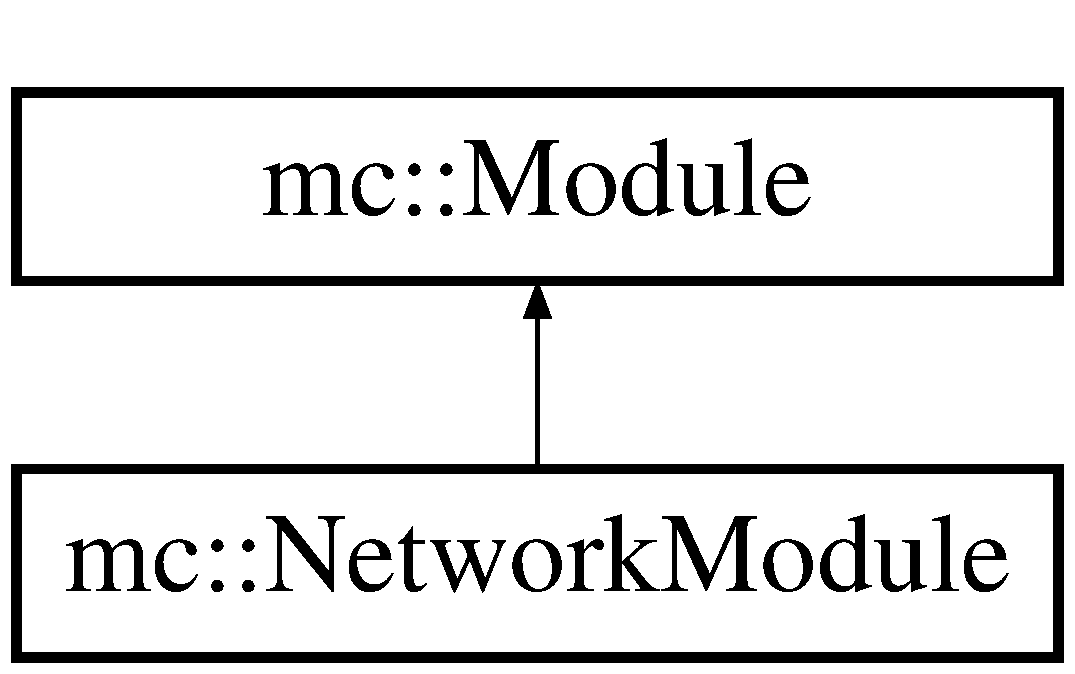
\includegraphics[height=2.000000cm]{classmc_1_1_network_module}
\end{center}
\end{figure}
\subsection*{Public Member Functions}
\begin{DoxyCompactItemize}
\item 
\hyperlink{_s_d_l__opengles2__gl2ext_8h_ae5d8fa23ad07c48bb609509eae494c95}{void} \hyperlink{classmc_1_1_network_module_ad5ec63cfdd43e8c4374dbbb65cfba3ff}{init} ()
\item 
\hyperlink{_s_d_l__opengles2__gl2ext_8h_ae5d8fa23ad07c48bb609509eae494c95}{void} \hyperlink{classmc_1_1_network_module_a8b9f81c3f101250c8b8e16b05434555e}{tick} ()
\item 
\hyperlink{_s_d_l__opengles2__gl2ext_8h_ae5d8fa23ad07c48bb609509eae494c95}{void} \hyperlink{classmc_1_1_network_module_a9cbb7fce204c10620ba2ba07f8f4a3a2}{destroy} ()
\item 
\hyperlink{_s_d_l__opengl__glext_8h_ae84541b4f3d8e1ea24ec0f466a8c568b}{std\+::string} \hyperlink{classmc_1_1_network_module_acf87542f4ba61dfe44c394da01ba8f4c}{get\+Name} () const 
\end{DoxyCompactItemize}
\subsection*{Additional Inherited Members}


\subsection{Member Function Documentation}
\index{mc\+::\+Network\+Module@{mc\+::\+Network\+Module}!destroy@{destroy}}
\index{destroy@{destroy}!mc\+::\+Network\+Module@{mc\+::\+Network\+Module}}
\subsubsection[{\texorpdfstring{destroy()}{destroy()}}]{\setlength{\rightskip}{0pt plus 5cm}{\bf void} mc\+::\+Network\+Module\+::destroy (
\begin{DoxyParamCaption}
{}
\end{DoxyParamCaption}
)\hspace{0.3cm}{\ttfamily [virtual]}}\hypertarget{classmc_1_1_network_module_a9cbb7fce204c10620ba2ba07f8f4a3a2}{}\label{classmc_1_1_network_module_a9cbb7fce204c10620ba2ba07f8f4a3a2}


Implements \hyperlink{classmc_1_1_module_abf13bd45de10185d4139dfff22a555d2}{mc\+::\+Module}.

\index{mc\+::\+Network\+Module@{mc\+::\+Network\+Module}!get\+Name@{get\+Name}}
\index{get\+Name@{get\+Name}!mc\+::\+Network\+Module@{mc\+::\+Network\+Module}}
\subsubsection[{\texorpdfstring{get\+Name() const }{getName() const }}]{\setlength{\rightskip}{0pt plus 5cm}{\bf std\+::string} mc\+::\+Network\+Module\+::get\+Name (
\begin{DoxyParamCaption}
{}
\end{DoxyParamCaption}
) const\hspace{0.3cm}{\ttfamily [virtual]}}\hypertarget{classmc_1_1_network_module_acf87542f4ba61dfe44c394da01ba8f4c}{}\label{classmc_1_1_network_module_acf87542f4ba61dfe44c394da01ba8f4c}


Implements \hyperlink{classmc_1_1_module_aa6d981a55ad5c04a39768e3ddcb0ad49}{mc\+::\+Module}.

\index{mc\+::\+Network\+Module@{mc\+::\+Network\+Module}!init@{init}}
\index{init@{init}!mc\+::\+Network\+Module@{mc\+::\+Network\+Module}}
\subsubsection[{\texorpdfstring{init()}{init()}}]{\setlength{\rightskip}{0pt plus 5cm}{\bf void} mc\+::\+Network\+Module\+::init (
\begin{DoxyParamCaption}
{}
\end{DoxyParamCaption}
)\hspace{0.3cm}{\ttfamily [virtual]}}\hypertarget{classmc_1_1_network_module_ad5ec63cfdd43e8c4374dbbb65cfba3ff}{}\label{classmc_1_1_network_module_ad5ec63cfdd43e8c4374dbbb65cfba3ff}


Implements \hyperlink{classmc_1_1_module_a854aad3bb8a2f60446fb14aeb28967b6}{mc\+::\+Module}.

\index{mc\+::\+Network\+Module@{mc\+::\+Network\+Module}!tick@{tick}}
\index{tick@{tick}!mc\+::\+Network\+Module@{mc\+::\+Network\+Module}}
\subsubsection[{\texorpdfstring{tick()}{tick()}}]{\setlength{\rightskip}{0pt plus 5cm}{\bf void} mc\+::\+Network\+Module\+::tick (
\begin{DoxyParamCaption}
{}
\end{DoxyParamCaption}
)}\hypertarget{classmc_1_1_network_module_a8b9f81c3f101250c8b8e16b05434555e}{}\label{classmc_1_1_network_module_a8b9f81c3f101250c8b8e16b05434555e}


The documentation for this class was generated from the following files\+:\begin{DoxyCompactItemize}
\item 
D\+:/\+Workspace/\+M\+A\+C\+E/\+M\+C-\/\+Network/\hyperlink{_network_8h}{Network.\+h}\item 
D\+:/\+Workspace/\+M\+A\+C\+E/\+M\+C-\/\+Network/\hyperlink{_network_8cpp}{Network.\+cpp}\end{DoxyCompactItemize}

\hypertarget{structmc_1_1_object_not_found_in_array}{}\section{mc\+:\+:Object\+Not\+Found\+In\+Array Struct Reference}
\label{structmc_1_1_object_not_found_in_array}\index{mc\+::\+Object\+Not\+Found\+In\+Array@{mc\+::\+Object\+Not\+Found\+In\+Array}}


{\ttfamily \#include $<$Exceptions.\+h$>$}

Inheritance diagram for mc\+:\+:Object\+Not\+Found\+In\+Array\+:\begin{figure}[H]
\begin{center}
\leavevmode
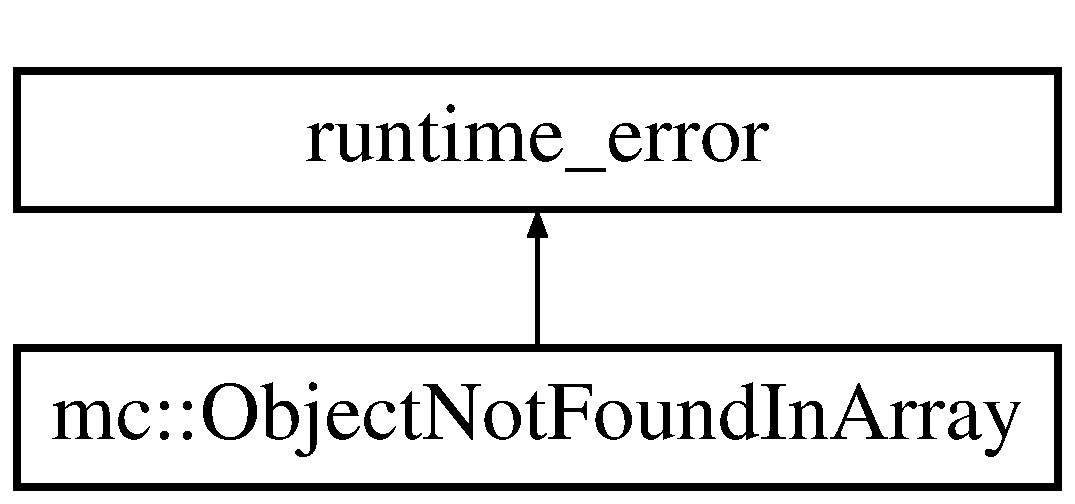
\includegraphics[height=2.000000cm]{structmc_1_1_object_not_found_in_array}
\end{center}
\end{figure}
\subsection*{Public Member Functions}
\begin{DoxyCompactItemize}
\item 
\hyperlink{structmc_1_1_object_not_found_in_array_accc8985a7187fbcf5fc78527bb17ac67}{Object\+Not\+Found\+In\+Array} (const char $\ast$\hyperlink{_s_d_l__opengl__glext_8h_a1f2d7f8147412c43ba2303a56f97ee73}{c}=\char`\"{}No \hyperlink{_s_d_l__opengl__glext_8h_a7b6161cffb9b8aee272b3b916183d28c}{message} was given\char`\"{})
\item 
\hyperlink{structmc_1_1_object_not_found_in_array_a3c5cd8e08030600a0c2bde64fada71cc}{Object\+Not\+Found\+In\+Array} (const \hyperlink{_s_d_l__opengl__glext_8h_ae84541b4f3d8e1ea24ec0f466a8c568b}{std\+::string} \hyperlink{_s_d_l__opengl__glext_8h_a1f2d7f8147412c43ba2303a56f97ee73}{c}=\char`\"{}No \hyperlink{_s_d_l__opengl__glext_8h_a7b6161cffb9b8aee272b3b916183d28c}{message} was given\char`\"{})
\end{DoxyCompactItemize}


\subsection{Constructor \& Destructor Documentation}
\index{mc\+::\+Object\+Not\+Found\+In\+Array@{mc\+::\+Object\+Not\+Found\+In\+Array}!Object\+Not\+Found\+In\+Array@{Object\+Not\+Found\+In\+Array}}
\index{Object\+Not\+Found\+In\+Array@{Object\+Not\+Found\+In\+Array}!mc\+::\+Object\+Not\+Found\+In\+Array@{mc\+::\+Object\+Not\+Found\+In\+Array}}
\subsubsection[{\texorpdfstring{Object\+Not\+Found\+In\+Array(const char $\ast$c=""No message was given"")}{ObjectNotFoundInArray(const char *c="No message was given")}}]{\setlength{\rightskip}{0pt plus 5cm}mc\+::\+Object\+Not\+Found\+In\+Array\+::\+Object\+Not\+Found\+In\+Array (
\begin{DoxyParamCaption}
\item[{const char $\ast$}]{c = {\ttfamily \char`\"{}No~{\bf message}~was~given\char`\"{}}}
\end{DoxyParamCaption}
)\hspace{0.3cm}{\ttfamily [inline]}, {\ttfamily [explicit]}}\hypertarget{structmc_1_1_object_not_found_in_array_accc8985a7187fbcf5fc78527bb17ac67}{}\label{structmc_1_1_object_not_found_in_array_accc8985a7187fbcf5fc78527bb17ac67}
\index{mc\+::\+Object\+Not\+Found\+In\+Array@{mc\+::\+Object\+Not\+Found\+In\+Array}!Object\+Not\+Found\+In\+Array@{Object\+Not\+Found\+In\+Array}}
\index{Object\+Not\+Found\+In\+Array@{Object\+Not\+Found\+In\+Array}!mc\+::\+Object\+Not\+Found\+In\+Array@{mc\+::\+Object\+Not\+Found\+In\+Array}}
\subsubsection[{\texorpdfstring{Object\+Not\+Found\+In\+Array(const std\+::string c=""No message was given"")}{ObjectNotFoundInArray(const std::string c="No message was given")}}]{\setlength{\rightskip}{0pt plus 5cm}mc\+::\+Object\+Not\+Found\+In\+Array\+::\+Object\+Not\+Found\+In\+Array (
\begin{DoxyParamCaption}
\item[{const {\bf std\+::string}}]{c = {\ttfamily \char`\"{}No~{\bf message}~was~given\char`\"{}}}
\end{DoxyParamCaption}
)\hspace{0.3cm}{\ttfamily [inline]}, {\ttfamily [explicit]}}\hypertarget{structmc_1_1_object_not_found_in_array_a3c5cd8e08030600a0c2bde64fada71cc}{}\label{structmc_1_1_object_not_found_in_array_a3c5cd8e08030600a0c2bde64fada71cc}


The documentation for this struct was generated from the following file\+:\begin{DoxyCompactItemize}
\item 
D\+:/\+Workspace/\+M\+A\+C\+E/\+M\+C-\/\+System/\hyperlink{_exceptions_8h}{Exceptions.\+h}\end{DoxyCompactItemize}

\hypertarget{classmc_1_1_position}{}\section{mc\+:\+:Position Class Reference}
\label{classmc_1_1_position}\index{mc\+::\+Position@{mc\+::\+Position}}


{\ttfamily \#include $<$Position.\+h$>$}

Inheritance diagram for mc\+:\+:Position\+:\begin{figure}[H]
\begin{center}
\leavevmode
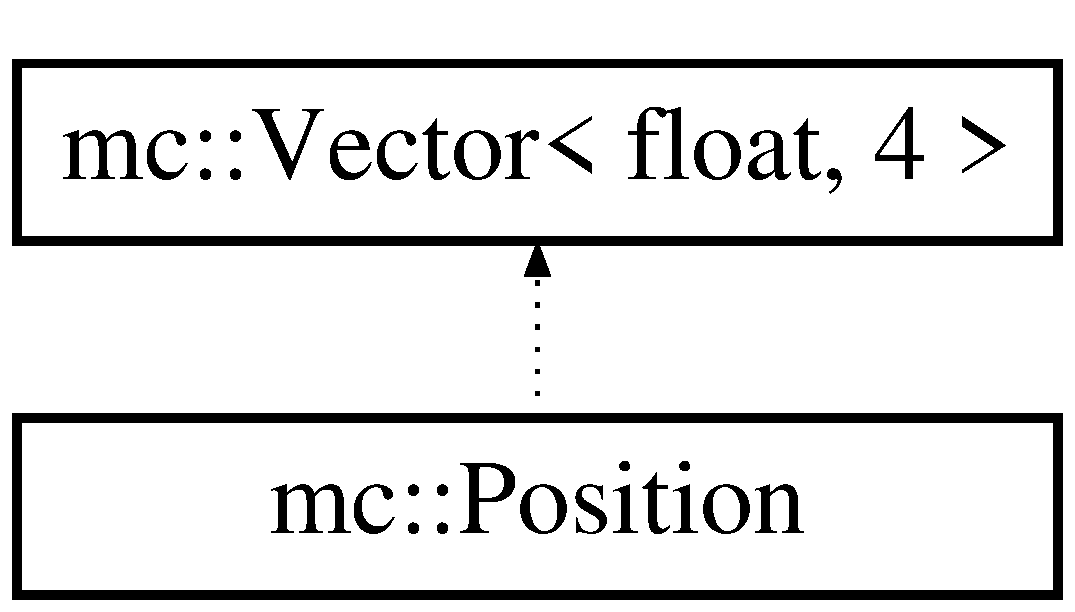
\includegraphics[height=2.000000cm]{d1/dbc/classmc_1_1_position}
\end{center}
\end{figure}


The documentation for this class was generated from the following file\+:\begin{DoxyCompactItemize}
\item 
D\+:/\+Workspace/\+M\+A\+C\+E/\+M\+C-\/\+System/\+Utility/\hyperlink{_position_8h}{Position.\+h}\end{DoxyCompactItemize}

\hypertarget{classmc_1_1_position_data}{}\section{mc\+:\+:Position\+Data Class Reference}
\label{classmc_1_1_position_data}\index{mc\+::\+Position\+Data@{mc\+::\+Position\+Data}}


{\ttfamily \#include $<$Position.\+h$>$}



The documentation for this class was generated from the following file\+:\begin{DoxyCompactItemize}
\item 
D\+:/\+Workspace/\+M\+A\+C\+E/\+M\+C-\/\+System/\+Utility/\hyperlink{_position_8h}{Position.\+h}\end{DoxyCompactItemize}

\hypertarget{classmc_1_1_sound}{}\section{mc\+:\+:Sound Class Reference}
\label{classmc_1_1_sound}\index{mc\+::\+Sound@{mc\+::\+Sound}}


{\ttfamily \#include $<$Sound.\+h$>$}

\subsection*{Public Member Functions}
\begin{DoxyCompactItemize}
\item 
\hyperlink{classmc_1_1_sound_aaa21de95445df04e711c104e7a281b20}{Sound} (const char $\ast$file)
\item 
void \hyperlink{classmc_1_1_sound_ada8c6c5ca032301f7d38aa7c996c0f9e}{play} ()
\item 
void \hyperlink{classmc_1_1_sound_a67dcafee2327b68452b091e13101fe92}{pause} ()
\item 
void \hyperlink{classmc_1_1_sound_a51548f5c106e154185347660e171133b}{stop} ()
\item 
void \hyperlink{classmc_1_1_sound_a6b18000746b1f6b5c5efedd58e864ab7}{rewind} ()
\item 
void \hyperlink{classmc_1_1_sound_a595bb512e1176165389897728366769c}{destroy} ()
\item 
void \hyperlink{classmc_1_1_sound_a2d22dfb3e3a0bc75c25ca0b9d9f19663}{set\+Gain} (float gain)
\item 
void \hyperlink{classmc_1_1_sound_ae38a4567c49eeb9f32239659874233c7}{set\+Pitch} (float pitch)
\item 
void \hyperlink{classmc_1_1_sound_af80534638f7aed8284514fed8352eec6}{set\+Looping} (bool looping)
\end{DoxyCompactItemize}


\subsection{Constructor \& Destructor Documentation}
\index{mc\+::\+Sound@{mc\+::\+Sound}!Sound@{Sound}}
\index{Sound@{Sound}!mc\+::\+Sound@{mc\+::\+Sound}}
\subsubsection[{\texorpdfstring{Sound(const char $\ast$file)}{Sound(const char *file)}}]{\setlength{\rightskip}{0pt plus 5cm}mc\+::\+Sound\+::\+Sound (
\begin{DoxyParamCaption}
\item[{const char $\ast$}]{file}
\end{DoxyParamCaption}
)}\hypertarget{classmc_1_1_sound_aaa21de95445df04e711c104e7a281b20}{}\label{classmc_1_1_sound_aaa21de95445df04e711c104e7a281b20}


\subsection{Member Function Documentation}
\index{mc\+::\+Sound@{mc\+::\+Sound}!destroy@{destroy}}
\index{destroy@{destroy}!mc\+::\+Sound@{mc\+::\+Sound}}
\subsubsection[{\texorpdfstring{destroy()}{destroy()}}]{\setlength{\rightskip}{0pt plus 5cm}void mc\+::\+Sound\+::destroy (
\begin{DoxyParamCaption}
{}
\end{DoxyParamCaption}
)}\hypertarget{classmc_1_1_sound_a595bb512e1176165389897728366769c}{}\label{classmc_1_1_sound_a595bb512e1176165389897728366769c}
\index{mc\+::\+Sound@{mc\+::\+Sound}!pause@{pause}}
\index{pause@{pause}!mc\+::\+Sound@{mc\+::\+Sound}}
\subsubsection[{\texorpdfstring{pause()}{pause()}}]{\setlength{\rightskip}{0pt plus 5cm}void mc\+::\+Sound\+::pause (
\begin{DoxyParamCaption}
{}
\end{DoxyParamCaption}
)}\hypertarget{classmc_1_1_sound_a67dcafee2327b68452b091e13101fe92}{}\label{classmc_1_1_sound_a67dcafee2327b68452b091e13101fe92}
\index{mc\+::\+Sound@{mc\+::\+Sound}!play@{play}}
\index{play@{play}!mc\+::\+Sound@{mc\+::\+Sound}}
\subsubsection[{\texorpdfstring{play()}{play()}}]{\setlength{\rightskip}{0pt plus 5cm}void mc\+::\+Sound\+::play (
\begin{DoxyParamCaption}
{}
\end{DoxyParamCaption}
)}\hypertarget{classmc_1_1_sound_ada8c6c5ca032301f7d38aa7c996c0f9e}{}\label{classmc_1_1_sound_ada8c6c5ca032301f7d38aa7c996c0f9e}
\index{mc\+::\+Sound@{mc\+::\+Sound}!rewind@{rewind}}
\index{rewind@{rewind}!mc\+::\+Sound@{mc\+::\+Sound}}
\subsubsection[{\texorpdfstring{rewind()}{rewind()}}]{\setlength{\rightskip}{0pt plus 5cm}void mc\+::\+Sound\+::rewind (
\begin{DoxyParamCaption}
{}
\end{DoxyParamCaption}
)}\hypertarget{classmc_1_1_sound_a6b18000746b1f6b5c5efedd58e864ab7}{}\label{classmc_1_1_sound_a6b18000746b1f6b5c5efedd58e864ab7}
\index{mc\+::\+Sound@{mc\+::\+Sound}!set\+Gain@{set\+Gain}}
\index{set\+Gain@{set\+Gain}!mc\+::\+Sound@{mc\+::\+Sound}}
\subsubsection[{\texorpdfstring{set\+Gain(float gain)}{setGain(float gain)}}]{\setlength{\rightskip}{0pt plus 5cm}void mc\+::\+Sound\+::set\+Gain (
\begin{DoxyParamCaption}
\item[{float}]{gain}
\end{DoxyParamCaption}
)}\hypertarget{classmc_1_1_sound_a2d22dfb3e3a0bc75c25ca0b9d9f19663}{}\label{classmc_1_1_sound_a2d22dfb3e3a0bc75c25ca0b9d9f19663}
\index{mc\+::\+Sound@{mc\+::\+Sound}!set\+Looping@{set\+Looping}}
\index{set\+Looping@{set\+Looping}!mc\+::\+Sound@{mc\+::\+Sound}}
\subsubsection[{\texorpdfstring{set\+Looping(bool looping)}{setLooping(bool looping)}}]{\setlength{\rightskip}{0pt plus 5cm}void mc\+::\+Sound\+::set\+Looping (
\begin{DoxyParamCaption}
\item[{bool}]{looping}
\end{DoxyParamCaption}
)}\hypertarget{classmc_1_1_sound_af80534638f7aed8284514fed8352eec6}{}\label{classmc_1_1_sound_af80534638f7aed8284514fed8352eec6}
\index{mc\+::\+Sound@{mc\+::\+Sound}!set\+Pitch@{set\+Pitch}}
\index{set\+Pitch@{set\+Pitch}!mc\+::\+Sound@{mc\+::\+Sound}}
\subsubsection[{\texorpdfstring{set\+Pitch(float pitch)}{setPitch(float pitch)}}]{\setlength{\rightskip}{0pt plus 5cm}void mc\+::\+Sound\+::set\+Pitch (
\begin{DoxyParamCaption}
\item[{float}]{pitch}
\end{DoxyParamCaption}
)}\hypertarget{classmc_1_1_sound_ae38a4567c49eeb9f32239659874233c7}{}\label{classmc_1_1_sound_ae38a4567c49eeb9f32239659874233c7}
\index{mc\+::\+Sound@{mc\+::\+Sound}!stop@{stop}}
\index{stop@{stop}!mc\+::\+Sound@{mc\+::\+Sound}}
\subsubsection[{\texorpdfstring{stop()}{stop()}}]{\setlength{\rightskip}{0pt plus 5cm}void mc\+::\+Sound\+::stop (
\begin{DoxyParamCaption}
{}
\end{DoxyParamCaption}
)}\hypertarget{classmc_1_1_sound_a51548f5c106e154185347660e171133b}{}\label{classmc_1_1_sound_a51548f5c106e154185347660e171133b}


The documentation for this class was generated from the following files\+:\begin{DoxyCompactItemize}
\item 
D\+:/\+Workspace/\+M\+A\+C\+E/\+M\+C-\/\+Audio/\hyperlink{_sound_8h}{Sound.\+h}\item 
D\+:/\+Workspace/\+M\+A\+C\+E/\+M\+C-\/\+Audio/\hyperlink{_sound_8cpp}{Sound.\+cpp}\end{DoxyCompactItemize}

\hypertarget{classmc_1_1_sound_manager}{}\section{mc\+:\+:Sound\+Manager Class Reference}
\label{classmc_1_1_sound_manager}\index{mc\+::\+Sound\+Manager@{mc\+::\+Sound\+Manager}}


{\ttfamily \#include $<$Sound\+Manager.\+h$>$}

\subsection*{Static Public Member Functions}
\begin{DoxyCompactItemize}
\item 
static \hyperlink{_s_d_l__opengles2__gl2ext_8h_ae5d8fa23ad07c48bb609509eae494c95}{void} \hyperlink{classmc_1_1_sound_manager_a430d3b6e3aabdd4b0b58a92fe1a5150e}{init} ()
\item 
static \hyperlink{_s_d_l__opengles2__gl2ext_8h_ae5d8fa23ad07c48bb609509eae494c95}{void} \hyperlink{classmc_1_1_sound_manager_a5f05665c3b5b197b186800cf25d820a1}{destroy} ()
\end{DoxyCompactItemize}


\subsection{Member Function Documentation}
\index{mc\+::\+Sound\+Manager@{mc\+::\+Sound\+Manager}!destroy@{destroy}}
\index{destroy@{destroy}!mc\+::\+Sound\+Manager@{mc\+::\+Sound\+Manager}}
\subsubsection[{\texorpdfstring{destroy()}{destroy()}}]{\setlength{\rightskip}{0pt plus 5cm}{\bf void} mc\+::\+Sound\+Manager\+::destroy (
\begin{DoxyParamCaption}
{}
\end{DoxyParamCaption}
)\hspace{0.3cm}{\ttfamily [static]}}\hypertarget{classmc_1_1_sound_manager_a5f05665c3b5b197b186800cf25d820a1}{}\label{classmc_1_1_sound_manager_a5f05665c3b5b197b186800cf25d820a1}
\index{mc\+::\+Sound\+Manager@{mc\+::\+Sound\+Manager}!init@{init}}
\index{init@{init}!mc\+::\+Sound\+Manager@{mc\+::\+Sound\+Manager}}
\subsubsection[{\texorpdfstring{init()}{init()}}]{\setlength{\rightskip}{0pt plus 5cm}{\bf void} mc\+::\+Sound\+Manager\+::init (
\begin{DoxyParamCaption}
{}
\end{DoxyParamCaption}
)\hspace{0.3cm}{\ttfamily [static]}}\hypertarget{classmc_1_1_sound_manager_a430d3b6e3aabdd4b0b58a92fe1a5150e}{}\label{classmc_1_1_sound_manager_a430d3b6e3aabdd4b0b58a92fe1a5150e}


The documentation for this class was generated from the following files\+:\begin{DoxyCompactItemize}
\item 
D\+:/\+Workspace/\+M\+A\+C\+E/\+M\+C-\/\+Audio/\hyperlink{_sound_manager_8h}{Sound\+Manager.\+h}\item 
D\+:/\+Workspace/\+M\+A\+C\+E/\+M\+C-\/\+Audio/\hyperlink{_sound_manager_8cpp}{Sound\+Manager.\+cpp}\end{DoxyCompactItemize}

\hypertarget{classmc_1_1_system}{}\section{mc\+:\+:System Class Reference}
\label{classmc_1_1_system}\index{mc\+::\+System@{mc\+::\+System}}


{\ttfamily \#include $<$System.\+h$>$}

\subsection*{Static Public Member Functions}
\begin{DoxyCompactItemize}
\item 
static \hyperlink{_s_d_l__thread_8h_a6a64f9be4433e4de6e2f2f548cf3c08e}{int} \hyperlink{classmc_1_1_system_a21a8af9fa9f4a2699478967cbb6949ee}{add\+Module} (\hyperlink{classmc_1_1_module}{Module} \&\hyperlink{_s_d_l__opengl__glext_8h_af593500c283bf1a787a6f947f503a5c2}{m})
\item 
static \hyperlink{_s_d_l__opengles2__gl2ext_8h_ae5d8fa23ad07c48bb609509eae494c95}{void} \hyperlink{classmc_1_1_system_ab37f8cd571040772e73a07584f8b0dba}{remove\+Module} (\hyperlink{classmc_1_1_module}{Module} \&\hyperlink{_s_d_l__opengl__glext_8h_af593500c283bf1a787a6f947f503a5c2}{m})
\item 
static \hyperlink{_s_d_l__opengles2__gl2ext_8h_ae5d8fa23ad07c48bb609509eae494c95}{void} \hyperlink{classmc_1_1_system_a08969e2d1572536469827e7b44e904f9}{remove\+Module} (\hyperlink{_s_d_l__opengl__glext_8h_ae84541b4f3d8e1ea24ec0f466a8c568b}{std\+::string} module)
\item 
static \hyperlink{_s_d_l__opengles2__gl2ext_8h_ae5d8fa23ad07c48bb609509eae494c95}{void} \hyperlink{classmc_1_1_system_aed18cf4077fa7c71432197597b190508}{remove\+Module} (\hyperlink{_s_d_l__thread_8h_a6a64f9be4433e4de6e2f2f548cf3c08e}{int} i)
\item 
static \hyperlink{classmc_1_1_module}{Module} $\ast$ \hyperlink{classmc_1_1_system_afb983a07b501764541c47a773e6044c8}{get\+Module} (\hyperlink{_s_d_l__opengl__glext_8h_ae84541b4f3d8e1ea24ec0f466a8c568b}{std\+::string} keyword)
\item 
static \hyperlink{classmc_1_1_module}{Module} $\ast$ \hyperlink{classmc_1_1_system_ad5f68cf3d76b080e10684a4a82e06abd}{get\+Module} (\hyperlink{_s_d_l__thread_8h_a6a64f9be4433e4de6e2f2f548cf3c08e}{int} i)
\item 
static bool \hyperlink{classmc_1_1_system_a8d33e21ec54da4940e14e7d1eb1a522b}{module\+Exists} (\hyperlink{_s_d_l__opengl__glext_8h_ae84541b4f3d8e1ea24ec0f466a8c568b}{std\+::string} module)
\item 
static bool \hyperlink{classmc_1_1_system_a16b15b813b7eb7dfbb84845bb4568f94}{module\+Exists} (\hyperlink{classmc_1_1_module}{Module} $\ast$module)
\item 
static \hyperlink{namespacemc_ad1c06461067735b3b17e0df612532c4e}{Size} \hyperlink{classmc_1_1_system_adf3dad3de5f7b16ccae9fd980ed2bcaf}{number\+Of\+Modules} ()
\item 
static \hyperlink{_s_d_l__opengles2__gl2ext_8h_ae5d8fa23ad07c48bb609509eae494c95}{void} \hyperlink{classmc_1_1_system_aa8164cbb910ce94ba763e7033ade380f}{assert\+Module} (\hyperlink{_s_d_l__opengl__glext_8h_ae84541b4f3d8e1ea24ec0f466a8c568b}{std\+::string} module, \hyperlink{_s_d_l__opengl__glext_8h_ae84541b4f3d8e1ea24ec0f466a8c568b}{std\+::string} error\+Message)
\item 
static \hyperlink{_s_d_l__opengles2__gl2ext_8h_ae5d8fa23ad07c48bb609509eae494c95}{void} \hyperlink{classmc_1_1_system_ae1828bcb4d2661c51e164ef986205a2c}{assert\+Module} (\hyperlink{_s_d_l__opengl__glext_8h_ae84541b4f3d8e1ea24ec0f466a8c568b}{std\+::string} module)
\item 
static \hyperlink{_s_d_l__opengles2__gl2ext_8h_ae5d8fa23ad07c48bb609509eae494c95}{void} \hyperlink{classmc_1_1_system_a86b7559895967af432c5c3db728bd0bc}{init} ()
\item 
static \hyperlink{_s_d_l__opengles2__gl2ext_8h_ae5d8fa23ad07c48bb609509eae494c95}{void} \hyperlink{classmc_1_1_system_a37d9b4e42bc96bddf835abd0bf3176bd}{terminate} ()
\item 
static \hyperlink{_s_d_l__opengles2__gl2ext_8h_ae5d8fa23ad07c48bb609509eae494c95}{void} \hyperlink{classmc_1_1_system_a90e14e44eb5a6019c913a6a197deb4a0}{update} ()
\end{DoxyCompactItemize}


\subsection{Member Function Documentation}
\index{mc\+::\+System@{mc\+::\+System}!add\+Module@{add\+Module}}
\index{add\+Module@{add\+Module}!mc\+::\+System@{mc\+::\+System}}
\subsubsection[{\texorpdfstring{add\+Module(\+Module \&m)}{addModule(Module &m)}}]{\setlength{\rightskip}{0pt plus 5cm}{\bf int} mc\+::\+System\+::add\+Module (
\begin{DoxyParamCaption}
\item[{{\bf Module} \&}]{m}
\end{DoxyParamCaption}
)\hspace{0.3cm}{\ttfamily [static]}}\hypertarget{classmc_1_1_system_a21a8af9fa9f4a2699478967cbb6949ee}{}\label{classmc_1_1_system_a21a8af9fa9f4a2699478967cbb6949ee}
\index{mc\+::\+System@{mc\+::\+System}!assert\+Module@{assert\+Module}}
\index{assert\+Module@{assert\+Module}!mc\+::\+System@{mc\+::\+System}}
\subsubsection[{\texorpdfstring{assert\+Module(std\+::string module, std\+::string error\+Message)}{assertModule(std::string module, std::string errorMessage)}}]{\setlength{\rightskip}{0pt plus 5cm}{\bf void} mc\+::\+System\+::assert\+Module (
\begin{DoxyParamCaption}
\item[{{\bf std\+::string}}]{module, }
\item[{{\bf std\+::string}}]{error\+Message}
\end{DoxyParamCaption}
)\hspace{0.3cm}{\ttfamily [static]}}\hypertarget{classmc_1_1_system_aa8164cbb910ce94ba763e7033ade380f}{}\label{classmc_1_1_system_aa8164cbb910ce94ba763e7033ade380f}
\index{mc\+::\+System@{mc\+::\+System}!assert\+Module@{assert\+Module}}
\index{assert\+Module@{assert\+Module}!mc\+::\+System@{mc\+::\+System}}
\subsubsection[{\texorpdfstring{assert\+Module(std\+::string module)}{assertModule(std::string module)}}]{\setlength{\rightskip}{0pt plus 5cm}{\bf void} mc\+::\+System\+::assert\+Module (
\begin{DoxyParamCaption}
\item[{{\bf std\+::string}}]{module}
\end{DoxyParamCaption}
)\hspace{0.3cm}{\ttfamily [static]}}\hypertarget{classmc_1_1_system_ae1828bcb4d2661c51e164ef986205a2c}{}\label{classmc_1_1_system_ae1828bcb4d2661c51e164ef986205a2c}
\index{mc\+::\+System@{mc\+::\+System}!get\+Module@{get\+Module}}
\index{get\+Module@{get\+Module}!mc\+::\+System@{mc\+::\+System}}
\subsubsection[{\texorpdfstring{get\+Module(std\+::string keyword)}{getModule(std::string keyword)}}]{\setlength{\rightskip}{0pt plus 5cm}{\bf Module} $\ast$ mc\+::\+System\+::get\+Module (
\begin{DoxyParamCaption}
\item[{{\bf std\+::string}}]{keyword}
\end{DoxyParamCaption}
)\hspace{0.3cm}{\ttfamily [static]}}\hypertarget{classmc_1_1_system_afb983a07b501764541c47a773e6044c8}{}\label{classmc_1_1_system_afb983a07b501764541c47a773e6044c8}
\index{mc\+::\+System@{mc\+::\+System}!get\+Module@{get\+Module}}
\index{get\+Module@{get\+Module}!mc\+::\+System@{mc\+::\+System}}
\subsubsection[{\texorpdfstring{get\+Module(int i)}{getModule(int i)}}]{\setlength{\rightskip}{0pt plus 5cm}{\bf Module} $\ast$ mc\+::\+System\+::get\+Module (
\begin{DoxyParamCaption}
\item[{{\bf int}}]{i}
\end{DoxyParamCaption}
)\hspace{0.3cm}{\ttfamily [static]}}\hypertarget{classmc_1_1_system_ad5f68cf3d76b080e10684a4a82e06abd}{}\label{classmc_1_1_system_ad5f68cf3d76b080e10684a4a82e06abd}
\index{mc\+::\+System@{mc\+::\+System}!init@{init}}
\index{init@{init}!mc\+::\+System@{mc\+::\+System}}
\subsubsection[{\texorpdfstring{init()}{init()}}]{\setlength{\rightskip}{0pt plus 5cm}{\bf void} mc\+::\+System\+::init (
\begin{DoxyParamCaption}
{}
\end{DoxyParamCaption}
)\hspace{0.3cm}{\ttfamily [static]}}\hypertarget{classmc_1_1_system_a86b7559895967af432c5c3db728bd0bc}{}\label{classmc_1_1_system_a86b7559895967af432c5c3db728bd0bc}
\index{mc\+::\+System@{mc\+::\+System}!module\+Exists@{module\+Exists}}
\index{module\+Exists@{module\+Exists}!mc\+::\+System@{mc\+::\+System}}
\subsubsection[{\texorpdfstring{module\+Exists(std\+::string module)}{moduleExists(std::string module)}}]{\setlength{\rightskip}{0pt plus 5cm}bool mc\+::\+System\+::module\+Exists (
\begin{DoxyParamCaption}
\item[{{\bf std\+::string}}]{module}
\end{DoxyParamCaption}
)\hspace{0.3cm}{\ttfamily [static]}}\hypertarget{classmc_1_1_system_a8d33e21ec54da4940e14e7d1eb1a522b}{}\label{classmc_1_1_system_a8d33e21ec54da4940e14e7d1eb1a522b}
\index{mc\+::\+System@{mc\+::\+System}!module\+Exists@{module\+Exists}}
\index{module\+Exists@{module\+Exists}!mc\+::\+System@{mc\+::\+System}}
\subsubsection[{\texorpdfstring{module\+Exists(\+Module $\ast$module)}{moduleExists(Module *module)}}]{\setlength{\rightskip}{0pt plus 5cm}bool mc\+::\+System\+::module\+Exists (
\begin{DoxyParamCaption}
\item[{{\bf Module} $\ast$}]{module}
\end{DoxyParamCaption}
)\hspace{0.3cm}{\ttfamily [static]}}\hypertarget{classmc_1_1_system_a16b15b813b7eb7dfbb84845bb4568f94}{}\label{classmc_1_1_system_a16b15b813b7eb7dfbb84845bb4568f94}
\index{mc\+::\+System@{mc\+::\+System}!number\+Of\+Modules@{number\+Of\+Modules}}
\index{number\+Of\+Modules@{number\+Of\+Modules}!mc\+::\+System@{mc\+::\+System}}
\subsubsection[{\texorpdfstring{number\+Of\+Modules()}{numberOfModules()}}]{\setlength{\rightskip}{0pt plus 5cm}{\bf Size} mc\+::\+System\+::number\+Of\+Modules (
\begin{DoxyParamCaption}
{}
\end{DoxyParamCaption}
)\hspace{0.3cm}{\ttfamily [static]}}\hypertarget{classmc_1_1_system_adf3dad3de5f7b16ccae9fd980ed2bcaf}{}\label{classmc_1_1_system_adf3dad3de5f7b16ccae9fd980ed2bcaf}
\index{mc\+::\+System@{mc\+::\+System}!remove\+Module@{remove\+Module}}
\index{remove\+Module@{remove\+Module}!mc\+::\+System@{mc\+::\+System}}
\subsubsection[{\texorpdfstring{remove\+Module(\+Module \&m)}{removeModule(Module &m)}}]{\setlength{\rightskip}{0pt plus 5cm}{\bf void} mc\+::\+System\+::remove\+Module (
\begin{DoxyParamCaption}
\item[{{\bf Module} \&}]{m}
\end{DoxyParamCaption}
)\hspace{0.3cm}{\ttfamily [static]}}\hypertarget{classmc_1_1_system_ab37f8cd571040772e73a07584f8b0dba}{}\label{classmc_1_1_system_ab37f8cd571040772e73a07584f8b0dba}
\index{mc\+::\+System@{mc\+::\+System}!remove\+Module@{remove\+Module}}
\index{remove\+Module@{remove\+Module}!mc\+::\+System@{mc\+::\+System}}
\subsubsection[{\texorpdfstring{remove\+Module(std\+::string module)}{removeModule(std::string module)}}]{\setlength{\rightskip}{0pt plus 5cm}{\bf void} mc\+::\+System\+::remove\+Module (
\begin{DoxyParamCaption}
\item[{{\bf std\+::string}}]{module}
\end{DoxyParamCaption}
)\hspace{0.3cm}{\ttfamily [static]}}\hypertarget{classmc_1_1_system_a08969e2d1572536469827e7b44e904f9}{}\label{classmc_1_1_system_a08969e2d1572536469827e7b44e904f9}
\index{mc\+::\+System@{mc\+::\+System}!remove\+Module@{remove\+Module}}
\index{remove\+Module@{remove\+Module}!mc\+::\+System@{mc\+::\+System}}
\subsubsection[{\texorpdfstring{remove\+Module(int i)}{removeModule(int i)}}]{\setlength{\rightskip}{0pt plus 5cm}{\bf void} mc\+::\+System\+::remove\+Module (
\begin{DoxyParamCaption}
\item[{{\bf int}}]{i}
\end{DoxyParamCaption}
)\hspace{0.3cm}{\ttfamily [static]}}\hypertarget{classmc_1_1_system_aed18cf4077fa7c71432197597b190508}{}\label{classmc_1_1_system_aed18cf4077fa7c71432197597b190508}
\index{mc\+::\+System@{mc\+::\+System}!terminate@{terminate}}
\index{terminate@{terminate}!mc\+::\+System@{mc\+::\+System}}
\subsubsection[{\texorpdfstring{terminate()}{terminate()}}]{\setlength{\rightskip}{0pt plus 5cm}{\bf void} mc\+::\+System\+::terminate (
\begin{DoxyParamCaption}
{}
\end{DoxyParamCaption}
)\hspace{0.3cm}{\ttfamily [static]}}\hypertarget{classmc_1_1_system_a37d9b4e42bc96bddf835abd0bf3176bd}{}\label{classmc_1_1_system_a37d9b4e42bc96bddf835abd0bf3176bd}
\index{mc\+::\+System@{mc\+::\+System}!update@{update}}
\index{update@{update}!mc\+::\+System@{mc\+::\+System}}
\subsubsection[{\texorpdfstring{update()}{update()}}]{\setlength{\rightskip}{0pt plus 5cm}{\bf void} mc\+::\+System\+::update (
\begin{DoxyParamCaption}
{}
\end{DoxyParamCaption}
)\hspace{0.3cm}{\ttfamily [static]}}\hypertarget{classmc_1_1_system_a90e14e44eb5a6019c913a6a197deb4a0}{}\label{classmc_1_1_system_a90e14e44eb5a6019c913a6a197deb4a0}


The documentation for this class was generated from the following files\+:\begin{DoxyCompactItemize}
\item 
D\+:/\+Workspace/\+M\+A\+C\+E/\+M\+C-\/\+System/\hyperlink{_system_8h}{System.\+h}\item 
D\+:/\+Workspace/\+M\+A\+C\+E/\+M\+C-\/\+System/\hyperlink{_system_8cpp}{System.\+cpp}\end{DoxyCompactItemize}

\hypertarget{classmc_1_1_tcp_server}{}\section{mc\+:\+:Tcp\+Server Class Reference}
\label{classmc_1_1_tcp_server}\index{mc\+::\+Tcp\+Server@{mc\+::\+Tcp\+Server}}


{\ttfamily \#include $<$Tcp\+Server.\+h$>$}

\subsection*{Public Member Functions}
\begin{DoxyCompactItemize}
\item 
\hyperlink{classmc_1_1_tcp_server_acbb28a8b861de2686f9f33e2808962c8}{Tcp\+Server} (int port)
\item 
void \hyperlink{classmc_1_1_tcp_server_a33697f2c1c5d422c78b6ae71a0b2e835}{accept} ()
\item 
void \hyperlink{classmc_1_1_tcp_server_a22520cd5e029fc7fd821170a540867c3}{destroy} ()
\end{DoxyCompactItemize}


\subsection{Constructor \& Destructor Documentation}
\index{mc\+::\+Tcp\+Server@{mc\+::\+Tcp\+Server}!Tcp\+Server@{Tcp\+Server}}
\index{Tcp\+Server@{Tcp\+Server}!mc\+::\+Tcp\+Server@{mc\+::\+Tcp\+Server}}
\subsubsection[{\texorpdfstring{Tcp\+Server(int port)}{TcpServer(int port)}}]{\setlength{\rightskip}{0pt plus 5cm}mc\+::\+Tcp\+Server\+::\+Tcp\+Server (
\begin{DoxyParamCaption}
\item[{int}]{port}
\end{DoxyParamCaption}
)}\hypertarget{classmc_1_1_tcp_server_acbb28a8b861de2686f9f33e2808962c8}{}\label{classmc_1_1_tcp_server_acbb28a8b861de2686f9f33e2808962c8}


\subsection{Member Function Documentation}
\index{mc\+::\+Tcp\+Server@{mc\+::\+Tcp\+Server}!accept@{accept}}
\index{accept@{accept}!mc\+::\+Tcp\+Server@{mc\+::\+Tcp\+Server}}
\subsubsection[{\texorpdfstring{accept()}{accept()}}]{\setlength{\rightskip}{0pt plus 5cm}void mc\+::\+Tcp\+Server\+::accept (
\begin{DoxyParamCaption}
{}
\end{DoxyParamCaption}
)}\hypertarget{classmc_1_1_tcp_server_a33697f2c1c5d422c78b6ae71a0b2e835}{}\label{classmc_1_1_tcp_server_a33697f2c1c5d422c78b6ae71a0b2e835}
\index{mc\+::\+Tcp\+Server@{mc\+::\+Tcp\+Server}!destroy@{destroy}}
\index{destroy@{destroy}!mc\+::\+Tcp\+Server@{mc\+::\+Tcp\+Server}}
\subsubsection[{\texorpdfstring{destroy()}{destroy()}}]{\setlength{\rightskip}{0pt plus 5cm}void mc\+::\+Tcp\+Server\+::destroy (
\begin{DoxyParamCaption}
{}
\end{DoxyParamCaption}
)}\hypertarget{classmc_1_1_tcp_server_a22520cd5e029fc7fd821170a540867c3}{}\label{classmc_1_1_tcp_server_a22520cd5e029fc7fd821170a540867c3}


The documentation for this class was generated from the following files\+:\begin{DoxyCompactItemize}
\item 
D\+:/\+Workspace/\+M\+A\+C\+E/\+M\+C-\/\+Network/tcp/\hyperlink{_tcp_server_8h}{Tcp\+Server.\+h}\item 
D\+:/\+Workspace/\+M\+A\+C\+E/\+M\+C-\/\+Network/tcp/\hyperlink{_tcp_server_8cpp}{Tcp\+Server.\+cpp}\end{DoxyCompactItemize}

\hypertarget{classmc_1_1_vector}{}\section{mc\+:\+:Vector$<$ T, N $>$ Class Template Reference}
\label{classmc_1_1_vector}\index{mc\+::\+Vector$<$ T, N $>$@{mc\+::\+Vector$<$ T, N $>$}}


Class that allows for vector math.  




{\ttfamily \#include $<$Vector.\+h$>$}

Inheritance diagram for mc\+:\+:Vector$<$ T, N $>$\+:\begin{figure}[H]
\begin{center}
\leavevmode
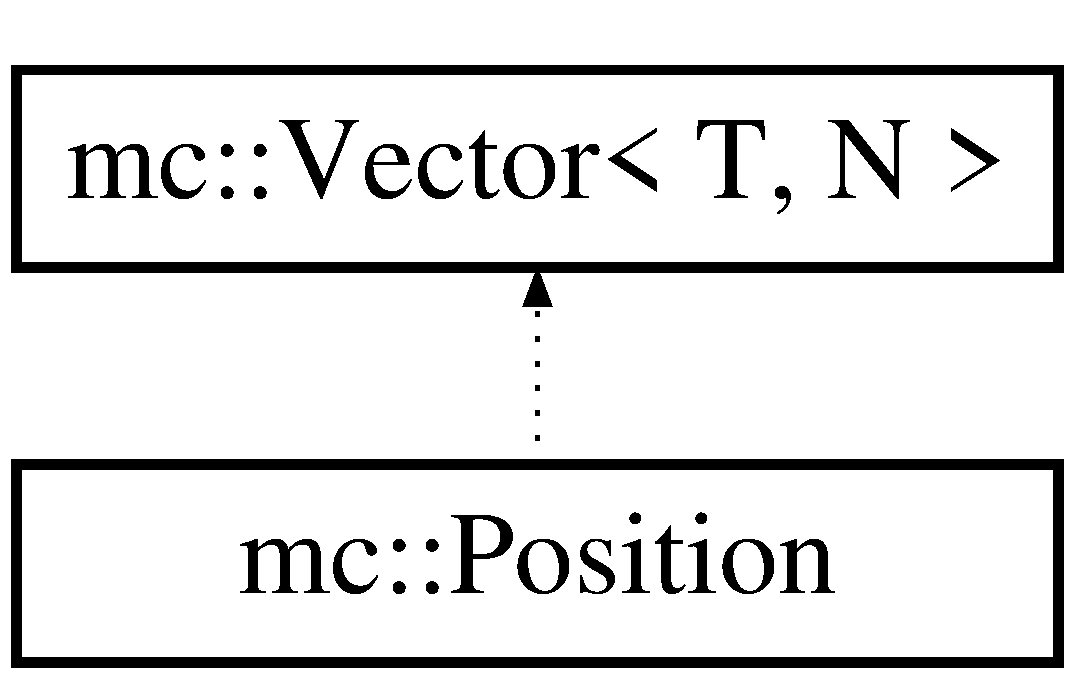
\includegraphics[height=2.000000cm]{classmc_1_1_vector}
\end{center}
\end{figure}
\subsection*{Public Member Functions}
\begin{DoxyCompactItemize}
\item 
\hyperlink{_s_d_l__opengl__glext_8h_a52f38e7d822a46377fde7a02708eedb1}{std\+::array}$<$ T, N $>$ \& \hyperlink{classmc_1_1_vector_ad8649fb50d1cebdc4f7e2886f445560a}{get\+Contents} ()
\item 
const \hyperlink{_s_d_l__opengl__glext_8h_a52f38e7d822a46377fde7a02708eedb1}{std\+::array}$<$ T, N $>$ \& \hyperlink{classmc_1_1_vector_ac312084ca4f2fe312eec6799df7e3f22}{get\+Contents} () const 
\item 
\hyperlink{_s_d_l__opengles2__gl2ext_8h_ae5d8fa23ad07c48bb609509eae494c95}{void} \hyperlink{classmc_1_1_vector_a2e674c851be8cf10808c86895e9ca86f}{set\+Contents} (const \hyperlink{_s_d_l__opengl__glext_8h_a52f38e7d822a46377fde7a02708eedb1}{std\+::array}$<$ T, N $>$ contents)
\item 
virtual unsigned \hyperlink{_s_d_l__thread_8h_a6a64f9be4433e4de6e2f2f548cf3c08e}{int} \hyperlink{classmc_1_1_vector_a85c37dc7b6c2ad12f5cab67d6db54b49}{size} () const 
\item 
T \& \hyperlink{classmc_1_1_vector_a3335869546b80addf0aafe5e009ffbde}{get} (unsigned i)
\item 
const T \& \hyperlink{classmc_1_1_vector_a58776300ccb5cac12fc04a24c9848053}{get} (unsigned \hyperlink{_s_d_l__thread_8h_a6a64f9be4433e4de6e2f2f548cf3c08e}{int} i) const 
\item 
\hyperlink{_s_d_l__opengles2__gl2ext_8h_ae5d8fa23ad07c48bb609509eae494c95}{void} \hyperlink{classmc_1_1_vector_a11e1f8cfd518752bb19b35437c66ee9d}{set} (unsigned \hyperlink{_s_d_l__thread_8h_a6a64f9be4433e4de6e2f2f548cf3c08e}{int} position, T \hyperlink{_s_d_l__opengl__glext_8h_a8ad81492d410ff2ac11f754f4042150f}{value})
\item 
T $\ast$ \hyperlink{classmc_1_1_vector_a1cb61e23c56abeb0b1d4c1a8b569e831}{begin} ()
\item 
T $\ast$ \hyperlink{classmc_1_1_vector_a728eef3a0e46669e5c7be8792a8b7b26}{end} ()
\item 
T \& \hyperlink{classmc_1_1_vector_a1113b584d428e6943e7ea23df89ef006}{operator\mbox{[}$\,$\mbox{]}} (\hyperlink{_s_d_l__thread_8h_a6a64f9be4433e4de6e2f2f548cf3c08e}{int} i)
\item 
const T \& \hyperlink{classmc_1_1_vector_a1bbd519ec7b6f6902ce81983478e3c92}{operator\mbox{[}$\,$\mbox{]}} (\hyperlink{_s_d_l__thread_8h_a6a64f9be4433e4de6e2f2f548cf3c08e}{int} i) const 
\item 
\hyperlink{classmc_1_1_vector}{Vector} \hyperlink{classmc_1_1_vector_a41f3ca26b2d43a91797df7499afcc5c5}{operator+} (const \hyperlink{classmc_1_1_vector}{Vector}$<$ T, N $>$ \&\hyperlink{_s_d_l__opengl__glext_8h_a5ffadbbacc6b89cf6218bc43b384d3fe}{right}) const 
\item 
\hyperlink{classmc_1_1_vector}{Vector} \hyperlink{classmc_1_1_vector_ac486a0798fd812967cb543c23bf60e3b}{operator-\/} (const \hyperlink{classmc_1_1_vector}{Vector}$<$ T, N $>$ \&\hyperlink{_s_d_l__opengl__glext_8h_a5ffadbbacc6b89cf6218bc43b384d3fe}{right}) const 
\item 
\hyperlink{classmc_1_1_vector}{Vector} \hyperlink{classmc_1_1_vector_a5760307dcf1bbc6ecbf4e576dc5c4838}{operator/} (const \hyperlink{classmc_1_1_vector}{Vector}$<$ T, N $>$ \&\hyperlink{_s_d_l__opengl__glext_8h_a5ffadbbacc6b89cf6218bc43b384d3fe}{right}) const 
\item 
\hyperlink{classmc_1_1_vector}{Vector} \hyperlink{classmc_1_1_vector_a64037e6603bb0f6997d1c2d22de2a4c9}{operator$\ast$} (const \hyperlink{classmc_1_1_vector}{Vector}$<$ T, N $>$ \&\hyperlink{_s_d_l__opengl__glext_8h_a5ffadbbacc6b89cf6218bc43b384d3fe}{right}) const 
\item 
{\footnotesize template$<$typename T\+Other , int N\+Other$>$ }\\bool \hyperlink{classmc_1_1_vector_a2f324924de53bc758f94df7b7b4e339b}{operator==} (const \hyperlink{classmc_1_1_vector}{Vector}$<$ T\+Other, N\+Other $>$ \&other)
\item 
{\footnotesize template$<$typename T\+Other , int N\+Other$>$ }\\bool \hyperlink{classmc_1_1_vector_aa45600b2bcd72732feb2f24d6c3e9ef6}{operator!=} (const \hyperlink{classmc_1_1_vector}{Vector}$<$ T\+Other, N\+Other $>$ \&other)
\item 
\hyperlink{classmc_1_1_vector}{Vector} \hyperlink{classmc_1_1_vector_af8000128edbd58d1790f23697501cd9d}{operator=} (T arr\mbox{[}N\mbox{]})
\item 
\hyperlink{classmc_1_1_vector_a05aed259e7ff40b4e6639f7dda5886cd}{Vector} (T arr\mbox{[}N\mbox{]})
\item 
\hyperlink{classmc_1_1_vector_a7c2fa3ae75ebb6d155aa3e3aa140ce09}{Vector} ()
\item 
\hyperlink{classmc_1_1_vector_a18dc923904b1d0511a9b9eefa72e8cb6}{Vector} (\hyperlink{_s_d_l__opengl__glext_8h_a52f38e7d822a46377fde7a02708eedb1}{std\+::array}$<$ T, N $>$ \&contents)
\item 
\hyperlink{classmc_1_1_vector_a9cd50db0b1a697ff4368a1072e99182d}{Vector} (const \hyperlink{classmc_1_1_vector}{Vector} \&\hyperlink{_s_d_l__opengl__glext_8h_a0c0d4701a6c89f4f7f0640715d27ab26}{obj})
\end{DoxyCompactItemize}
\subsection*{Protected Attributes}
\begin{DoxyCompactItemize}
\item 
\hyperlink{_s_d_l__opengl__glext_8h_a52f38e7d822a46377fde7a02708eedb1}{std\+::array}$<$ T, N $>$ \hyperlink{classmc_1_1_vector_a2f84e2ba450c97ace26007263a1a4313}{content}
\end{DoxyCompactItemize}


\subsection{Detailed Description}
\subsubsection*{template$<$typename T, int N$>$\\*
class mc\+::\+Vector$<$ T, N $>$}

Class that allows for vector math. 


\begin{DoxyTemplParams}{Template Parameters}
{\em T} & what the
\begin{DoxyCode}
\hyperlink{classmc_1_1_vector_a7c2fa3ae75ebb6d155aa3e3aa140ce09}{Vector} 
\end{DoxyCode}
 is made of and calculates with. \\
\hline
{\em N} & width of the
\begin{DoxyCode}
\hyperlink{classmc_1_1_vector_a7c2fa3ae75ebb6d155aa3e3aa140ce09}{Vector} 
\end{DoxyCode}
 \\
\hline
\end{DoxyTemplParams}


\subsection{Constructor \& Destructor Documentation}
\index{mc\+::\+Vector@{mc\+::\+Vector}!Vector@{Vector}}
\index{Vector@{Vector}!mc\+::\+Vector@{mc\+::\+Vector}}
\subsubsection[{\texorpdfstring{Vector(\+T arr[N])}{Vector(T arr[N])}}]{\setlength{\rightskip}{0pt plus 5cm}template$<$typename T, int N$>$ {\bf mc\+::\+Vector}$<$ T, N $>$\+::{\bf Vector} (
\begin{DoxyParamCaption}
\item[{T}]{arr\mbox{[}\+N\mbox{]}}
\end{DoxyParamCaption}
)\hspace{0.3cm}{\ttfamily [inline]}}\hypertarget{classmc_1_1_vector_a05aed259e7ff40b4e6639f7dda5886cd}{}\label{classmc_1_1_vector_a05aed259e7ff40b4e6639f7dda5886cd}
\index{mc\+::\+Vector@{mc\+::\+Vector}!Vector@{Vector}}
\index{Vector@{Vector}!mc\+::\+Vector@{mc\+::\+Vector}}
\subsubsection[{\texorpdfstring{Vector()}{Vector()}}]{\setlength{\rightskip}{0pt plus 5cm}template$<$typename T, int N$>$ {\bf mc\+::\+Vector}$<$ T, N $>$\+::{\bf Vector} (
\begin{DoxyParamCaption}
{}
\end{DoxyParamCaption}
)\hspace{0.3cm}{\ttfamily [inline]}}\hypertarget{classmc_1_1_vector_a7c2fa3ae75ebb6d155aa3e3aa140ce09}{}\label{classmc_1_1_vector_a7c2fa3ae75ebb6d155aa3e3aa140ce09}
\index{mc\+::\+Vector@{mc\+::\+Vector}!Vector@{Vector}}
\index{Vector@{Vector}!mc\+::\+Vector@{mc\+::\+Vector}}
\subsubsection[{\texorpdfstring{Vector(std\+::array$<$ T, N $>$ \&contents)}{Vector(std::array< T, N > &contents)}}]{\setlength{\rightskip}{0pt plus 5cm}template$<$typename T, int N$>$ {\bf mc\+::\+Vector}$<$ T, N $>$\+::{\bf Vector} (
\begin{DoxyParamCaption}
\item[{{\bf std\+::array}$<$ T, N $>$ \&}]{contents}
\end{DoxyParamCaption}
)\hspace{0.3cm}{\ttfamily [inline]}}\hypertarget{classmc_1_1_vector_a18dc923904b1d0511a9b9eefa72e8cb6}{}\label{classmc_1_1_vector_a18dc923904b1d0511a9b9eefa72e8cb6}
\index{mc\+::\+Vector@{mc\+::\+Vector}!Vector@{Vector}}
\index{Vector@{Vector}!mc\+::\+Vector@{mc\+::\+Vector}}
\subsubsection[{\texorpdfstring{Vector(const Vector \&obj)}{Vector(const Vector &obj)}}]{\setlength{\rightskip}{0pt plus 5cm}template$<$typename T, int N$>$ {\bf mc\+::\+Vector}$<$ T, N $>$\+::{\bf Vector} (
\begin{DoxyParamCaption}
\item[{const {\bf Vector}$<$ T, N $>$ \&}]{obj}
\end{DoxyParamCaption}
)\hspace{0.3cm}{\ttfamily [inline]}}\hypertarget{classmc_1_1_vector_a9cd50db0b1a697ff4368a1072e99182d}{}\label{classmc_1_1_vector_a9cd50db0b1a697ff4368a1072e99182d}


\subsection{Member Function Documentation}
\index{mc\+::\+Vector@{mc\+::\+Vector}!begin@{begin}}
\index{begin@{begin}!mc\+::\+Vector@{mc\+::\+Vector}}
\subsubsection[{\texorpdfstring{begin()}{begin()}}]{\setlength{\rightskip}{0pt plus 5cm}template$<$typename T, int N$>$ T$\ast$ {\bf mc\+::\+Vector}$<$ T, N $>$\+::begin (
\begin{DoxyParamCaption}
{}
\end{DoxyParamCaption}
)\hspace{0.3cm}{\ttfamily [inline]}}\hypertarget{classmc_1_1_vector_a1cb61e23c56abeb0b1d4c1a8b569e831}{}\label{classmc_1_1_vector_a1cb61e23c56abeb0b1d4c1a8b569e831}
\index{mc\+::\+Vector@{mc\+::\+Vector}!end@{end}}
\index{end@{end}!mc\+::\+Vector@{mc\+::\+Vector}}
\subsubsection[{\texorpdfstring{end()}{end()}}]{\setlength{\rightskip}{0pt plus 5cm}template$<$typename T, int N$>$ T$\ast$ {\bf mc\+::\+Vector}$<$ T, N $>$\+::{\bf end} (
\begin{DoxyParamCaption}
{}
\end{DoxyParamCaption}
)\hspace{0.3cm}{\ttfamily [inline]}}\hypertarget{classmc_1_1_vector_a728eef3a0e46669e5c7be8792a8b7b26}{}\label{classmc_1_1_vector_a728eef3a0e46669e5c7be8792a8b7b26}
\index{mc\+::\+Vector@{mc\+::\+Vector}!get@{get}}
\index{get@{get}!mc\+::\+Vector@{mc\+::\+Vector}}
\subsubsection[{\texorpdfstring{get(unsigned i)}{get(unsigned i)}}]{\setlength{\rightskip}{0pt plus 5cm}template$<$typename T, int N$>$ T\& {\bf mc\+::\+Vector}$<$ T, N $>$\+::get (
\begin{DoxyParamCaption}
\item[{unsigned}]{i}
\end{DoxyParamCaption}
)\hspace{0.3cm}{\ttfamily [inline]}}\hypertarget{classmc_1_1_vector_a3335869546b80addf0aafe5e009ffbde}{}\label{classmc_1_1_vector_a3335869546b80addf0aafe5e009ffbde}
\index{mc\+::\+Vector@{mc\+::\+Vector}!get@{get}}
\index{get@{get}!mc\+::\+Vector@{mc\+::\+Vector}}
\subsubsection[{\texorpdfstring{get(unsigned int i) const }{get(unsigned int i) const }}]{\setlength{\rightskip}{0pt plus 5cm}template$<$typename T, int N$>$ const T\& {\bf mc\+::\+Vector}$<$ T, N $>$\+::get (
\begin{DoxyParamCaption}
\item[{unsigned {\bf int}}]{i}
\end{DoxyParamCaption}
) const\hspace{0.3cm}{\ttfamily [inline]}}\hypertarget{classmc_1_1_vector_a58776300ccb5cac12fc04a24c9848053}{}\label{classmc_1_1_vector_a58776300ccb5cac12fc04a24c9848053}
\index{mc\+::\+Vector@{mc\+::\+Vector}!get\+Contents@{get\+Contents}}
\index{get\+Contents@{get\+Contents}!mc\+::\+Vector@{mc\+::\+Vector}}
\subsubsection[{\texorpdfstring{get\+Contents()}{getContents()}}]{\setlength{\rightskip}{0pt plus 5cm}template$<$typename T, int N$>$ {\bf std\+::array}$<$ T, N$>$\& {\bf mc\+::\+Vector}$<$ T, N $>$\+::get\+Contents (
\begin{DoxyParamCaption}
{}
\end{DoxyParamCaption}
)\hspace{0.3cm}{\ttfamily [inline]}}\hypertarget{classmc_1_1_vector_ad8649fb50d1cebdc4f7e2886f445560a}{}\label{classmc_1_1_vector_ad8649fb50d1cebdc4f7e2886f445560a}
\index{mc\+::\+Vector@{mc\+::\+Vector}!get\+Contents@{get\+Contents}}
\index{get\+Contents@{get\+Contents}!mc\+::\+Vector@{mc\+::\+Vector}}
\subsubsection[{\texorpdfstring{get\+Contents() const }{getContents() const }}]{\setlength{\rightskip}{0pt plus 5cm}template$<$typename T, int N$>$ const {\bf std\+::array}$<$ T,N$>$\& {\bf mc\+::\+Vector}$<$ T, N $>$\+::get\+Contents (
\begin{DoxyParamCaption}
{}
\end{DoxyParamCaption}
) const\hspace{0.3cm}{\ttfamily [inline]}}\hypertarget{classmc_1_1_vector_ac312084ca4f2fe312eec6799df7e3f22}{}\label{classmc_1_1_vector_ac312084ca4f2fe312eec6799df7e3f22}
\index{mc\+::\+Vector@{mc\+::\+Vector}!operator"!=@{operator"!=}}
\index{operator"!=@{operator"!=}!mc\+::\+Vector@{mc\+::\+Vector}}
\subsubsection[{\texorpdfstring{operator"!=(const Vector$<$ T\+Other, N\+Other $>$ \&other)}{operator!=(const Vector< TOther, NOther > &other)}}]{\setlength{\rightskip}{0pt plus 5cm}template$<$typename T, int N$>$ template$<$typename T\+Other , int N\+Other$>$ bool {\bf mc\+::\+Vector}$<$ T, N $>$\+::operator!= (
\begin{DoxyParamCaption}
\item[{const {\bf Vector}$<$ T\+Other, N\+Other $>$ \&}]{other}
\end{DoxyParamCaption}
)\hspace{0.3cm}{\ttfamily [inline]}}\hypertarget{classmc_1_1_vector_aa45600b2bcd72732feb2f24d6c3e9ef6}{}\label{classmc_1_1_vector_aa45600b2bcd72732feb2f24d6c3e9ef6}
\index{mc\+::\+Vector@{mc\+::\+Vector}!operator$\ast$@{operator$\ast$}}
\index{operator$\ast$@{operator$\ast$}!mc\+::\+Vector@{mc\+::\+Vector}}
\subsubsection[{\texorpdfstring{operator$\ast$(const Vector$<$ T, N $>$ \&right) const }{operator*(const Vector< T, N > &right) const }}]{\setlength{\rightskip}{0pt plus 5cm}template$<$typename T, int N$>$ {\bf Vector} {\bf mc\+::\+Vector}$<$ T, N $>$\+::operator$\ast$ (
\begin{DoxyParamCaption}
\item[{const {\bf Vector}$<$ T, N $>$ \&}]{right}
\end{DoxyParamCaption}
) const\hspace{0.3cm}{\ttfamily [inline]}}\hypertarget{classmc_1_1_vector_a64037e6603bb0f6997d1c2d22de2a4c9}{}\label{classmc_1_1_vector_a64037e6603bb0f6997d1c2d22de2a4c9}
\index{mc\+::\+Vector@{mc\+::\+Vector}!operator+@{operator+}}
\index{operator+@{operator+}!mc\+::\+Vector@{mc\+::\+Vector}}
\subsubsection[{\texorpdfstring{operator+(const Vector$<$ T, N $>$ \&right) const }{operator+(const Vector< T, N > &right) const }}]{\setlength{\rightskip}{0pt plus 5cm}template$<$typename T, int N$>$ {\bf Vector} {\bf mc\+::\+Vector}$<$ T, N $>$\+::operator+ (
\begin{DoxyParamCaption}
\item[{const {\bf Vector}$<$ T, N $>$ \&}]{right}
\end{DoxyParamCaption}
) const\hspace{0.3cm}{\ttfamily [inline]}}\hypertarget{classmc_1_1_vector_a41f3ca26b2d43a91797df7499afcc5c5}{}\label{classmc_1_1_vector_a41f3ca26b2d43a91797df7499afcc5c5}
\index{mc\+::\+Vector@{mc\+::\+Vector}!operator-\/@{operator-\/}}
\index{operator-\/@{operator-\/}!mc\+::\+Vector@{mc\+::\+Vector}}
\subsubsection[{\texorpdfstring{operator-\/(const Vector$<$ T, N $>$ \&right) const }{operator-(const Vector< T, N > &right) const }}]{\setlength{\rightskip}{0pt plus 5cm}template$<$typename T, int N$>$ {\bf Vector} {\bf mc\+::\+Vector}$<$ T, N $>$\+::operator-\/ (
\begin{DoxyParamCaption}
\item[{const {\bf Vector}$<$ T, N $>$ \&}]{right}
\end{DoxyParamCaption}
) const\hspace{0.3cm}{\ttfamily [inline]}}\hypertarget{classmc_1_1_vector_ac486a0798fd812967cb543c23bf60e3b}{}\label{classmc_1_1_vector_ac486a0798fd812967cb543c23bf60e3b}
\index{mc\+::\+Vector@{mc\+::\+Vector}!operator/@{operator/}}
\index{operator/@{operator/}!mc\+::\+Vector@{mc\+::\+Vector}}
\subsubsection[{\texorpdfstring{operator/(const Vector$<$ T, N $>$ \&right) const }{operator/(const Vector< T, N > &right) const }}]{\setlength{\rightskip}{0pt plus 5cm}template$<$typename T, int N$>$ {\bf Vector} {\bf mc\+::\+Vector}$<$ T, N $>$\+::operator/ (
\begin{DoxyParamCaption}
\item[{const {\bf Vector}$<$ T, N $>$ \&}]{right}
\end{DoxyParamCaption}
) const\hspace{0.3cm}{\ttfamily [inline]}}\hypertarget{classmc_1_1_vector_a5760307dcf1bbc6ecbf4e576dc5c4838}{}\label{classmc_1_1_vector_a5760307dcf1bbc6ecbf4e576dc5c4838}
\index{mc\+::\+Vector@{mc\+::\+Vector}!operator=@{operator=}}
\index{operator=@{operator=}!mc\+::\+Vector@{mc\+::\+Vector}}
\subsubsection[{\texorpdfstring{operator=(\+T arr[N])}{operator=(T arr[N])}}]{\setlength{\rightskip}{0pt plus 5cm}template$<$typename T, int N$>$ {\bf Vector} {\bf mc\+::\+Vector}$<$ T, N $>$\+::operator= (
\begin{DoxyParamCaption}
\item[{T}]{arr\mbox{[}\+N\mbox{]}}
\end{DoxyParamCaption}
)\hspace{0.3cm}{\ttfamily [inline]}}\hypertarget{classmc_1_1_vector_af8000128edbd58d1790f23697501cd9d}{}\label{classmc_1_1_vector_af8000128edbd58d1790f23697501cd9d}
\index{mc\+::\+Vector@{mc\+::\+Vector}!operator==@{operator==}}
\index{operator==@{operator==}!mc\+::\+Vector@{mc\+::\+Vector}}
\subsubsection[{\texorpdfstring{operator==(const Vector$<$ T\+Other, N\+Other $>$ \&other)}{operator==(const Vector< TOther, NOther > &other)}}]{\setlength{\rightskip}{0pt plus 5cm}template$<$typename T, int N$>$ template$<$typename T\+Other , int N\+Other$>$ bool {\bf mc\+::\+Vector}$<$ T, N $>$\+::operator== (
\begin{DoxyParamCaption}
\item[{const {\bf Vector}$<$ T\+Other, N\+Other $>$ \&}]{other}
\end{DoxyParamCaption}
)\hspace{0.3cm}{\ttfamily [inline]}}\hypertarget{classmc_1_1_vector_a2f324924de53bc758f94df7b7b4e339b}{}\label{classmc_1_1_vector_a2f324924de53bc758f94df7b7b4e339b}
\index{mc\+::\+Vector@{mc\+::\+Vector}!operator\mbox{[}$\,$\mbox{]}@{operator[]}}
\index{operator\mbox{[}$\,$\mbox{]}@{operator[]}!mc\+::\+Vector@{mc\+::\+Vector}}
\subsubsection[{\texorpdfstring{operator[](int i)}{operator[](int i)}}]{\setlength{\rightskip}{0pt plus 5cm}template$<$typename T, int N$>$ T\& {\bf mc\+::\+Vector}$<$ T, N $>$\+::operator\mbox{[}$\,$\mbox{]} (
\begin{DoxyParamCaption}
\item[{{\bf int}}]{i}
\end{DoxyParamCaption}
)\hspace{0.3cm}{\ttfamily [inline]}}\hypertarget{classmc_1_1_vector_a1113b584d428e6943e7ea23df89ef006}{}\label{classmc_1_1_vector_a1113b584d428e6943e7ea23df89ef006}
\index{mc\+::\+Vector@{mc\+::\+Vector}!operator\mbox{[}$\,$\mbox{]}@{operator[]}}
\index{operator\mbox{[}$\,$\mbox{]}@{operator[]}!mc\+::\+Vector@{mc\+::\+Vector}}
\subsubsection[{\texorpdfstring{operator[](int i) const }{operator[](int i) const }}]{\setlength{\rightskip}{0pt plus 5cm}template$<$typename T, int N$>$ const T\& {\bf mc\+::\+Vector}$<$ T, N $>$\+::operator\mbox{[}$\,$\mbox{]} (
\begin{DoxyParamCaption}
\item[{{\bf int}}]{i}
\end{DoxyParamCaption}
) const\hspace{0.3cm}{\ttfamily [inline]}}\hypertarget{classmc_1_1_vector_a1bbd519ec7b6f6902ce81983478e3c92}{}\label{classmc_1_1_vector_a1bbd519ec7b6f6902ce81983478e3c92}
\index{mc\+::\+Vector@{mc\+::\+Vector}!set@{set}}
\index{set@{set}!mc\+::\+Vector@{mc\+::\+Vector}}
\subsubsection[{\texorpdfstring{set(unsigned int position, T value)}{set(unsigned int position, T value)}}]{\setlength{\rightskip}{0pt plus 5cm}template$<$typename T, int N$>$ {\bf void} {\bf mc\+::\+Vector}$<$ T, N $>$\+::set (
\begin{DoxyParamCaption}
\item[{unsigned {\bf int}}]{position, }
\item[{T}]{value}
\end{DoxyParamCaption}
)\hspace{0.3cm}{\ttfamily [inline]}}\hypertarget{classmc_1_1_vector_a11e1f8cfd518752bb19b35437c66ee9d}{}\label{classmc_1_1_vector_a11e1f8cfd518752bb19b35437c66ee9d}
\index{mc\+::\+Vector@{mc\+::\+Vector}!set\+Contents@{set\+Contents}}
\index{set\+Contents@{set\+Contents}!mc\+::\+Vector@{mc\+::\+Vector}}
\subsubsection[{\texorpdfstring{set\+Contents(const std\+::array$<$ T, N $>$ contents)}{setContents(const std::array< T, N > contents)}}]{\setlength{\rightskip}{0pt plus 5cm}template$<$typename T, int N$>$ {\bf void} {\bf mc\+::\+Vector}$<$ T, N $>$\+::set\+Contents (
\begin{DoxyParamCaption}
\item[{const {\bf std\+::array}$<$ T, N $>$}]{contents}
\end{DoxyParamCaption}
)\hspace{0.3cm}{\ttfamily [inline]}}\hypertarget{classmc_1_1_vector_a2e674c851be8cf10808c86895e9ca86f}{}\label{classmc_1_1_vector_a2e674c851be8cf10808c86895e9ca86f}
\index{mc\+::\+Vector@{mc\+::\+Vector}!size@{size}}
\index{size@{size}!mc\+::\+Vector@{mc\+::\+Vector}}
\subsubsection[{\texorpdfstring{size() const }{size() const }}]{\setlength{\rightskip}{0pt plus 5cm}template$<$typename T, int N$>$ virtual unsigned {\bf int} {\bf mc\+::\+Vector}$<$ T, N $>$\+::{\bf size} (
\begin{DoxyParamCaption}
{}
\end{DoxyParamCaption}
) const\hspace{0.3cm}{\ttfamily [inline]}, {\ttfamily [virtual]}}\hypertarget{classmc_1_1_vector_a85c37dc7b6c2ad12f5cab67d6db54b49}{}\label{classmc_1_1_vector_a85c37dc7b6c2ad12f5cab67d6db54b49}


\subsection{Member Data Documentation}
\index{mc\+::\+Vector@{mc\+::\+Vector}!content@{content}}
\index{content@{content}!mc\+::\+Vector@{mc\+::\+Vector}}
\subsubsection[{\texorpdfstring{content}{content}}]{\setlength{\rightskip}{0pt plus 5cm}template$<$typename T, int N$>$ {\bf std\+::array}$<$T,N$>$ {\bf mc\+::\+Vector}$<$ T, N $>$\+::content\hspace{0.3cm}{\ttfamily [protected]}}\hypertarget{classmc_1_1_vector_a2f84e2ba450c97ace26007263a1a4313}{}\label{classmc_1_1_vector_a2f84e2ba450c97ace26007263a1a4313}


The documentation for this class was generated from the following file\+:\begin{DoxyCompactItemize}
\item 
D\+:/\+Workspace/\+M\+A\+C\+E/\+M\+C-\/\+System/\+Utility/\hyperlink{_vector_8h}{Vector.\+h}\end{DoxyCompactItemize}

\hypertarget{classmc_1_1_window}{}\section{mc\+:\+:Window Class Reference}
\label{classmc_1_1_window}\index{mc\+::\+Window@{mc\+::\+Window}}


{\ttfamily \#include $<$Window.\+h$>$}

\subsection*{Public Member Functions}
\begin{DoxyCompactItemize}
\item 
\hyperlink{classmc_1_1_window_a55f349e85260b2cab01941534df62954}{Window} (int width, int height, const char $\ast$title)
\item 
bool \hyperlink{classmc_1_1_window_acefbda4736db354ba98cef6d6489a0f1}{is\+Open} ()
\item 
S\+D\+L\+\_\+\+Window $\ast$ \hyperlink{classmc_1_1_window_a741a653af7b767e39a1d517fd1844674}{get\+S\+D\+L\+Window} ()
\item 
virtual void \hyperlink{classmc_1_1_window_ac9844e316c03c49e69528bd3a345a58d}{create} ()
\item 
virtual void \hyperlink{classmc_1_1_window_a2f62d5937f19a26c0d8349efd1ce75bd}{destroy} ()
\end{DoxyCompactItemize}
\subsection*{Protected Attributes}
\begin{DoxyCompactItemize}
\item 
S\+D\+L\+\_\+\+Window $\ast$ \hyperlink{classmc_1_1_window_a8df84ee7c278f016ef13ac0ede008f7c}{m\+\_\+window}
\item 
int \hyperlink{classmc_1_1_window_a1f4c4744822006d438a532282d2b36c5}{m\+\_\+original\+Width}
\item 
int \hyperlink{classmc_1_1_window_aef96e2ff220e319a9a87cf4ced39ddaf}{m\+\_\+original\+Height}
\item 
char $\ast$ \hyperlink{classmc_1_1_window_a27f0a568dfe2d21915debc0672dd072e}{m\+\_\+title}
\end{DoxyCompactItemize}
\subsection*{Friends}
\begin{DoxyCompactItemize}
\item 
class \hyperlink{classmc_1_1_window_a832d299d0131fc9740d25c15c804e42e}{Window\+Module}
\end{DoxyCompactItemize}


\subsection{Constructor \& Destructor Documentation}
\index{mc\+::\+Window@{mc\+::\+Window}!Window@{Window}}
\index{Window@{Window}!mc\+::\+Window@{mc\+::\+Window}}
\subsubsection[{\texorpdfstring{Window(int width, int height, const char $\ast$title)}{Window(int width, int height, const char *title)}}]{\setlength{\rightskip}{0pt plus 5cm}mc\+::\+Window\+::\+Window (
\begin{DoxyParamCaption}
\item[{int}]{width, }
\item[{int}]{height, }
\item[{const char $\ast$}]{title}
\end{DoxyParamCaption}
)}\hypertarget{classmc_1_1_window_a55f349e85260b2cab01941534df62954}{}\label{classmc_1_1_window_a55f349e85260b2cab01941534df62954}


\subsection{Member Function Documentation}
\index{mc\+::\+Window@{mc\+::\+Window}!create@{create}}
\index{create@{create}!mc\+::\+Window@{mc\+::\+Window}}
\subsubsection[{\texorpdfstring{create()}{create()}}]{\setlength{\rightskip}{0pt plus 5cm}void mc\+::\+Window\+::create (
\begin{DoxyParamCaption}
{}
\end{DoxyParamCaption}
)\hspace{0.3cm}{\ttfamily [virtual]}}\hypertarget{classmc_1_1_window_ac9844e316c03c49e69528bd3a345a58d}{}\label{classmc_1_1_window_ac9844e316c03c49e69528bd3a345a58d}
\index{mc\+::\+Window@{mc\+::\+Window}!destroy@{destroy}}
\index{destroy@{destroy}!mc\+::\+Window@{mc\+::\+Window}}
\subsubsection[{\texorpdfstring{destroy()}{destroy()}}]{\setlength{\rightskip}{0pt plus 5cm}void mc\+::\+Window\+::destroy (
\begin{DoxyParamCaption}
{}
\end{DoxyParamCaption}
)\hspace{0.3cm}{\ttfamily [virtual]}}\hypertarget{classmc_1_1_window_a2f62d5937f19a26c0d8349efd1ce75bd}{}\label{classmc_1_1_window_a2f62d5937f19a26c0d8349efd1ce75bd}
\index{mc\+::\+Window@{mc\+::\+Window}!get\+S\+D\+L\+Window@{get\+S\+D\+L\+Window}}
\index{get\+S\+D\+L\+Window@{get\+S\+D\+L\+Window}!mc\+::\+Window@{mc\+::\+Window}}
\subsubsection[{\texorpdfstring{get\+S\+D\+L\+Window()}{getSDLWindow()}}]{\setlength{\rightskip}{0pt plus 5cm}S\+D\+L\+\_\+\+Window $\ast$ mc\+::\+Window\+::get\+S\+D\+L\+Window (
\begin{DoxyParamCaption}
{}
\end{DoxyParamCaption}
)}\hypertarget{classmc_1_1_window_a741a653af7b767e39a1d517fd1844674}{}\label{classmc_1_1_window_a741a653af7b767e39a1d517fd1844674}
\index{mc\+::\+Window@{mc\+::\+Window}!is\+Open@{is\+Open}}
\index{is\+Open@{is\+Open}!mc\+::\+Window@{mc\+::\+Window}}
\subsubsection[{\texorpdfstring{is\+Open()}{isOpen()}}]{\setlength{\rightskip}{0pt plus 5cm}bool mc\+::\+Window\+::is\+Open (
\begin{DoxyParamCaption}
{}
\end{DoxyParamCaption}
)}\hypertarget{classmc_1_1_window_acefbda4736db354ba98cef6d6489a0f1}{}\label{classmc_1_1_window_acefbda4736db354ba98cef6d6489a0f1}


\subsection{Friends And Related Function Documentation}
\index{mc\+::\+Window@{mc\+::\+Window}!Window\+Module@{Window\+Module}}
\index{Window\+Module@{Window\+Module}!mc\+::\+Window@{mc\+::\+Window}}
\subsubsection[{\texorpdfstring{Window\+Module}{WindowModule}}]{\setlength{\rightskip}{0pt plus 5cm}friend class {\bf Window\+Module}\hspace{0.3cm}{\ttfamily [friend]}}\hypertarget{classmc_1_1_window_a832d299d0131fc9740d25c15c804e42e}{}\label{classmc_1_1_window_a832d299d0131fc9740d25c15c804e42e}


\subsection{Member Data Documentation}
\index{mc\+::\+Window@{mc\+::\+Window}!m\+\_\+original\+Height@{m\+\_\+original\+Height}}
\index{m\+\_\+original\+Height@{m\+\_\+original\+Height}!mc\+::\+Window@{mc\+::\+Window}}
\subsubsection[{\texorpdfstring{m\+\_\+original\+Height}{m_originalHeight}}]{\setlength{\rightskip}{0pt plus 5cm}int mc\+::\+Window\+::m\+\_\+original\+Height\hspace{0.3cm}{\ttfamily [protected]}}\hypertarget{classmc_1_1_window_aef96e2ff220e319a9a87cf4ced39ddaf}{}\label{classmc_1_1_window_aef96e2ff220e319a9a87cf4ced39ddaf}
\index{mc\+::\+Window@{mc\+::\+Window}!m\+\_\+original\+Width@{m\+\_\+original\+Width}}
\index{m\+\_\+original\+Width@{m\+\_\+original\+Width}!mc\+::\+Window@{mc\+::\+Window}}
\subsubsection[{\texorpdfstring{m\+\_\+original\+Width}{m_originalWidth}}]{\setlength{\rightskip}{0pt plus 5cm}int mc\+::\+Window\+::m\+\_\+original\+Width\hspace{0.3cm}{\ttfamily [protected]}}\hypertarget{classmc_1_1_window_a1f4c4744822006d438a532282d2b36c5}{}\label{classmc_1_1_window_a1f4c4744822006d438a532282d2b36c5}
\index{mc\+::\+Window@{mc\+::\+Window}!m\+\_\+title@{m\+\_\+title}}
\index{m\+\_\+title@{m\+\_\+title}!mc\+::\+Window@{mc\+::\+Window}}
\subsubsection[{\texorpdfstring{m\+\_\+title}{m_title}}]{\setlength{\rightskip}{0pt plus 5cm}char$\ast$ mc\+::\+Window\+::m\+\_\+title\hspace{0.3cm}{\ttfamily [protected]}}\hypertarget{classmc_1_1_window_a27f0a568dfe2d21915debc0672dd072e}{}\label{classmc_1_1_window_a27f0a568dfe2d21915debc0672dd072e}
\index{mc\+::\+Window@{mc\+::\+Window}!m\+\_\+window@{m\+\_\+window}}
\index{m\+\_\+window@{m\+\_\+window}!mc\+::\+Window@{mc\+::\+Window}}
\subsubsection[{\texorpdfstring{m\+\_\+window}{m_window}}]{\setlength{\rightskip}{0pt plus 5cm}S\+D\+L\+\_\+\+Window$\ast$ mc\+::\+Window\+::m\+\_\+window\hspace{0.3cm}{\ttfamily [protected]}}\hypertarget{classmc_1_1_window_a8df84ee7c278f016ef13ac0ede008f7c}{}\label{classmc_1_1_window_a8df84ee7c278f016ef13ac0ede008f7c}


The documentation for this class was generated from the following files\+:\begin{DoxyCompactItemize}
\item 
D\+:/\+Workspace/\+M\+A\+C\+E/\+M\+C-\/\+Window/\hyperlink{_window_8h}{Window.\+h}\item 
D\+:/\+Workspace/\+M\+A\+C\+E/\+M\+C-\/\+Window/\hyperlink{_window_8cpp}{Window.\+cpp}\end{DoxyCompactItemize}

\hypertarget{classmc_1_1_window_module}{}\section{mc\+:\+:Window\+Module Class Reference}
\label{classmc_1_1_window_module}\index{mc\+::\+Window\+Module@{mc\+::\+Window\+Module}}


{\ttfamily \#include $<$Window\+Module.\+h$>$}

Inheritance diagram for mc\+:\+:Window\+Module\+:\begin{figure}[H]
\begin{center}
\leavevmode
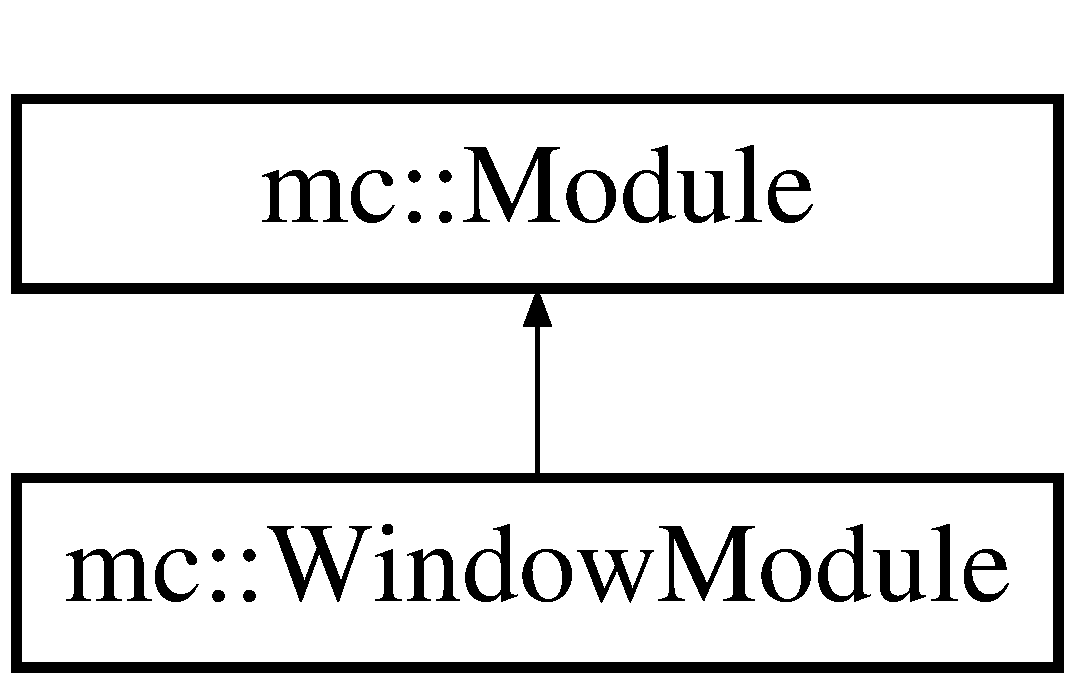
\includegraphics[height=2.000000cm]{classmc_1_1_window_module}
\end{center}
\end{figure}
\subsection*{Public Member Functions}
\begin{DoxyCompactItemize}
\item 
\hyperlink{classmc_1_1_window_module_a85f94176313ad80fde169a9034e75c78}{Window\+Module} ()
\item 
\hyperlink{_s_d_l__opengles2__gl2ext_8h_ae5d8fa23ad07c48bb609509eae494c95}{void} \hyperlink{classmc_1_1_window_module_acdc406a66ee7ab44277953b8429642ca}{init} ()
\item 
\hyperlink{_s_d_l__opengles2__gl2ext_8h_ae5d8fa23ad07c48bb609509eae494c95}{void} \hyperlink{classmc_1_1_window_module_ab9f6b46fe2624f52ed69188d5be94066}{tick} ()
\item 
\hyperlink{_s_d_l__opengles2__gl2ext_8h_ae5d8fa23ad07c48bb609509eae494c95}{void} \hyperlink{classmc_1_1_window_module_a4ad68d037b1ed9aa8740d01a0c2f3762}{destroy} ()
\item 
\hyperlink{_s_d_l__opengl__glext_8h_ae84541b4f3d8e1ea24ec0f466a8c568b}{std\+::string} \hyperlink{classmc_1_1_window_module_a69600ab76f3427c509594916abde0d37}{get\+Name} () const 
\end{DoxyCompactItemize}
\subsection*{Additional Inherited Members}


\subsection{Constructor \& Destructor Documentation}
\index{mc\+::\+Window\+Module@{mc\+::\+Window\+Module}!Window\+Module@{Window\+Module}}
\index{Window\+Module@{Window\+Module}!mc\+::\+Window\+Module@{mc\+::\+Window\+Module}}
\subsubsection[{\texorpdfstring{Window\+Module()}{WindowModule()}}]{\setlength{\rightskip}{0pt plus 5cm}mc\+::\+Window\+Module\+::\+Window\+Module (
\begin{DoxyParamCaption}
{}
\end{DoxyParamCaption}
)}\hypertarget{classmc_1_1_window_module_a85f94176313ad80fde169a9034e75c78}{}\label{classmc_1_1_window_module_a85f94176313ad80fde169a9034e75c78}


\subsection{Member Function Documentation}
\index{mc\+::\+Window\+Module@{mc\+::\+Window\+Module}!destroy@{destroy}}
\index{destroy@{destroy}!mc\+::\+Window\+Module@{mc\+::\+Window\+Module}}
\subsubsection[{\texorpdfstring{destroy()}{destroy()}}]{\setlength{\rightskip}{0pt plus 5cm}{\bf void} mc\+::\+Window\+Module\+::destroy (
\begin{DoxyParamCaption}
{}
\end{DoxyParamCaption}
)\hspace{0.3cm}{\ttfamily [virtual]}}\hypertarget{classmc_1_1_window_module_a4ad68d037b1ed9aa8740d01a0c2f3762}{}\label{classmc_1_1_window_module_a4ad68d037b1ed9aa8740d01a0c2f3762}


Implements \hyperlink{classmc_1_1_module_abf13bd45de10185d4139dfff22a555d2}{mc\+::\+Module}.

\index{mc\+::\+Window\+Module@{mc\+::\+Window\+Module}!get\+Name@{get\+Name}}
\index{get\+Name@{get\+Name}!mc\+::\+Window\+Module@{mc\+::\+Window\+Module}}
\subsubsection[{\texorpdfstring{get\+Name() const }{getName() const }}]{\setlength{\rightskip}{0pt plus 5cm}{\bf std\+::string} mc\+::\+Window\+Module\+::get\+Name (
\begin{DoxyParamCaption}
{}
\end{DoxyParamCaption}
) const\hspace{0.3cm}{\ttfamily [virtual]}}\hypertarget{classmc_1_1_window_module_a69600ab76f3427c509594916abde0d37}{}\label{classmc_1_1_window_module_a69600ab76f3427c509594916abde0d37}


Implements \hyperlink{classmc_1_1_module_aa6d981a55ad5c04a39768e3ddcb0ad49}{mc\+::\+Module}.

\index{mc\+::\+Window\+Module@{mc\+::\+Window\+Module}!init@{init}}
\index{init@{init}!mc\+::\+Window\+Module@{mc\+::\+Window\+Module}}
\subsubsection[{\texorpdfstring{init()}{init()}}]{\setlength{\rightskip}{0pt plus 5cm}{\bf void} mc\+::\+Window\+Module\+::init (
\begin{DoxyParamCaption}
{}
\end{DoxyParamCaption}
)\hspace{0.3cm}{\ttfamily [virtual]}}\hypertarget{classmc_1_1_window_module_acdc406a66ee7ab44277953b8429642ca}{}\label{classmc_1_1_window_module_acdc406a66ee7ab44277953b8429642ca}


Implements \hyperlink{classmc_1_1_module_a854aad3bb8a2f60446fb14aeb28967b6}{mc\+::\+Module}.

\index{mc\+::\+Window\+Module@{mc\+::\+Window\+Module}!tick@{tick}}
\index{tick@{tick}!mc\+::\+Window\+Module@{mc\+::\+Window\+Module}}
\subsubsection[{\texorpdfstring{tick()}{tick()}}]{\setlength{\rightskip}{0pt plus 5cm}{\bf void} mc\+::\+Window\+Module\+::tick (
\begin{DoxyParamCaption}
{}
\end{DoxyParamCaption}
)}\hypertarget{classmc_1_1_window_module_ab9f6b46fe2624f52ed69188d5be94066}{}\label{classmc_1_1_window_module_ab9f6b46fe2624f52ed69188d5be94066}


The documentation for this class was generated from the following files\+:\begin{DoxyCompactItemize}
\item 
D\+:/\+Workspace/\+M\+A\+C\+E/\+M\+C-\/\+Window/\hyperlink{_window_module_8h}{Window\+Module.\+h}\item 
D\+:/\+Workspace/\+M\+A\+C\+E/\+M\+C-\/\+Window/\hyperlink{_window_module_8cpp}{Window\+Module.\+cpp}\end{DoxyCompactItemize}

\chapter{File Documentation}
\hypertarget{_l_i_c_e_n_s_e_8md}{}\section{D\+:/\+Workspace/\+M\+A\+C\+E/\+L\+I\+C\+E\+N\+SE.md File Reference}
\label{_l_i_c_e_n_s_e_8md}\index{D\+:/\+Workspace/\+M\+A\+C\+E/\+L\+I\+C\+E\+N\+S\+E.\+md@{D\+:/\+Workspace/\+M\+A\+C\+E/\+L\+I\+C\+E\+N\+S\+E.\+md}}

\hypertarget{_sound_8cpp}{}\section{D\+:/\+Workspace/\+M\+A\+C\+E/\+M\+C-\/\+Audio/\+Sound.cpp File Reference}
\label{_sound_8cpp}\index{D\+:/\+Workspace/\+M\+A\+C\+E/\+M\+C-\/\+Audio/\+Sound.\+cpp@{D\+:/\+Workspace/\+M\+A\+C\+E/\+M\+C-\/\+Audio/\+Sound.\+cpp}}
{\ttfamily \#include $<$M\+C-\/\+Audio/\+Sound.\+h$>$}\\*
\subsection*{Namespaces}
\begin{DoxyCompactItemize}
\item 
 \hyperlink{namespacemc}{mc}
\end{DoxyCompactItemize}

\hypertarget{_sound_8h}{}\section{D\+:/\+Workspace/\+M\+A\+C\+E/\+M\+C-\/\+Audio/\+Sound.h File Reference}
\label{_sound_8h}\index{D\+:/\+Workspace/\+M\+A\+C\+E/\+M\+C-\/\+Audio/\+Sound.\+h@{D\+:/\+Workspace/\+M\+A\+C\+E/\+M\+C-\/\+Audio/\+Sound.\+h}}
{\ttfamily \#include $<$S\+D\+L/\+S\+D\+L\+\_\+mixer.\+h$>$}\\*
{\ttfamily \#include $<$A\+L/al.\+h$>$}\\*
{\ttfamily \#include $<$iostream$>$}\\*
\subsection*{Classes}
\begin{DoxyCompactItemize}
\item 
class \hyperlink{classmc_1_1_sound}{mc\+::\+Sound}
\end{DoxyCompactItemize}
\subsection*{Namespaces}
\begin{DoxyCompactItemize}
\item 
 \hyperlink{namespacemc}{mc}
\end{DoxyCompactItemize}

\hypertarget{_sound_manager_8cpp}{}\section{D\+:/\+Workspace/\+M\+A\+C\+E/\+M\+C-\/\+Audio/\+Sound\+Manager.cpp File Reference}
\label{_sound_manager_8cpp}\index{D\+:/\+Workspace/\+M\+A\+C\+E/\+M\+C-\/\+Audio/\+Sound\+Manager.\+cpp@{D\+:/\+Workspace/\+M\+A\+C\+E/\+M\+C-\/\+Audio/\+Sound\+Manager.\+cpp}}
{\ttfamily \#include $<$M\+C-\/\+Audio/\+Sound\+Manager.\+h$>$}\\*
\subsection*{Namespaces}
\begin{DoxyCompactItemize}
\item 
 \hyperlink{namespacemc}{mc}
\end{DoxyCompactItemize}

\hypertarget{_sound_manager_8h}{}\section{D\+:/\+Workspace/\+M\+A\+C\+E/\+M\+C-\/\+Audio/\+Sound\+Manager.h File Reference}
\label{_sound_manager_8h}\index{D\+:/\+Workspace/\+M\+A\+C\+E/\+M\+C-\/\+Audio/\+Sound\+Manager.\+h@{D\+:/\+Workspace/\+M\+A\+C\+E/\+M\+C-\/\+Audio/\+Sound\+Manager.\+h}}
{\ttfamily \#include $<$S\+D\+L/\+S\+D\+L\+\_\+mixer.\+h$>$}\\*
{\ttfamily \#include $<$A\+L/alc.\+h$>$}\\*
\subsection*{Classes}
\begin{DoxyCompactItemize}
\item 
class \hyperlink{classmc_1_1_sound_manager}{mc\+::\+Sound\+Manager}
\end{DoxyCompactItemize}
\subsection*{Namespaces}
\begin{DoxyCompactItemize}
\item 
 \hyperlink{namespacemc}{mc}
\end{DoxyCompactItemize}

\hypertarget{_graphics_8cpp}{}\section{D\+:/\+Workspace/\+M\+A\+C\+E/\+M\+C-\/\+Graphics/\+Graphics.cpp File Reference}
\label{_graphics_8cpp}\index{D\+:/\+Workspace/\+M\+A\+C\+E/\+M\+C-\/\+Graphics/\+Graphics.\+cpp@{D\+:/\+Workspace/\+M\+A\+C\+E/\+M\+C-\/\+Graphics/\+Graphics.\+cpp}}
{\ttfamily \#include $<$M\+C-\/\+Graphics/\+Graphics.\+h$>$}\\*
{\ttfamily \#include $<$iostream$>$}\\*
\subsection*{Namespaces}
\begin{DoxyCompactItemize}
\item 
 \hyperlink{namespacemc}{mc}
\end{DoxyCompactItemize}

\hypertarget{_graphics_8h}{}\section{D\+:/\+Workspace/\+M\+A\+C\+E/\+M\+C-\/\+Graphics/\+Graphics.h File Reference}
\label{_graphics_8h}\index{D\+:/\+Workspace/\+M\+A\+C\+E/\+M\+C-\/\+Graphics/\+Graphics.\+h@{D\+:/\+Workspace/\+M\+A\+C\+E/\+M\+C-\/\+Graphics/\+Graphics.\+h}}
{\ttfamily \#include $<$M\+C-\/\+System/\+System.\+h$>$}\\*
\subsection*{Classes}
\begin{DoxyCompactItemize}
\item 
class \hyperlink{classmc_1_1_graphics_module}{mc\+::\+Graphics\+Module}
\end{DoxyCompactItemize}
\subsection*{Namespaces}
\begin{DoxyCompactItemize}
\item 
 \hyperlink{namespacemc}{mc}
\end{DoxyCompactItemize}

\hypertarget{_network_8cpp}{}\section{D\+:/\+Workspace/\+M\+A\+C\+E/\+M\+C-\/\+Network/\+Network.cpp File Reference}
\label{_network_8cpp}\index{D\+:/\+Workspace/\+M\+A\+C\+E/\+M\+C-\/\+Network/\+Network.\+cpp@{D\+:/\+Workspace/\+M\+A\+C\+E/\+M\+C-\/\+Network/\+Network.\+cpp}}
{\ttfamily \#include $<$M\+C-\/\+Network/\+Network.\+h$>$}\\*
\subsection*{Namespaces}
\begin{DoxyCompactItemize}
\item 
 \hyperlink{namespacemc}{mc}
\end{DoxyCompactItemize}

\hypertarget{_network_8h}{}\section{D\+:/\+Workspace/\+M\+A\+C\+E/\+M\+C-\/\+Network/\+Network.h File Reference}
\label{_network_8h}\index{D\+:/\+Workspace/\+M\+A\+C\+E/\+M\+C-\/\+Network/\+Network.\+h@{D\+:/\+Workspace/\+M\+A\+C\+E/\+M\+C-\/\+Network/\+Network.\+h}}
{\ttfamily \#include $<$M\+C-\/\+System/\+System.\+h$>$}\\*
{\ttfamily \#include $<$S\+D\+L/\+S\+D\+L\+\_\+net.\+h$>$}\\*
\subsection*{Classes}
\begin{DoxyCompactItemize}
\item 
class \hyperlink{classmc_1_1_network_module}{mc\+::\+Network\+Module}
\end{DoxyCompactItemize}
\subsection*{Namespaces}
\begin{DoxyCompactItemize}
\item 
 \hyperlink{namespacemc}{mc}
\end{DoxyCompactItemize}

\hypertarget{_tcp_server_8cpp}{}\section{D\+:/\+Workspace/\+M\+A\+C\+E/\+M\+C-\/\+Network/tcp/\+Tcp\+Server.cpp File Reference}
\label{_tcp_server_8cpp}\index{D\+:/\+Workspace/\+M\+A\+C\+E/\+M\+C-\/\+Network/tcp/\+Tcp\+Server.\+cpp@{D\+:/\+Workspace/\+M\+A\+C\+E/\+M\+C-\/\+Network/tcp/\+Tcp\+Server.\+cpp}}
{\ttfamily \#include $<$M\+C-\/\+Network/tcp/\+Tcp\+Server.\+h$>$}\\*
\subsection*{Namespaces}
\begin{DoxyCompactItemize}
\item 
 \hyperlink{namespacemc}{mc}
\end{DoxyCompactItemize}

\hypertarget{_tcp_server_8h}{}\section{D\+:/\+Workspace/\+M\+A\+C\+E/\+M\+C-\/\+Network/tcp/\+Tcp\+Server.h File Reference}
\label{_tcp_server_8h}\index{D\+:/\+Workspace/\+M\+A\+C\+E/\+M\+C-\/\+Network/tcp/\+Tcp\+Server.\+h@{D\+:/\+Workspace/\+M\+A\+C\+E/\+M\+C-\/\+Network/tcp/\+Tcp\+Server.\+h}}
{\ttfamily \#include $<$S\+D\+L/\+S\+D\+L\+\_\+net.\+h$>$}\\*
{\ttfamily \#include $<$cstring$>$}\\*
{\ttfamily \#include $<$iostream$>$}\\*
\subsection*{Classes}
\begin{DoxyCompactItemize}
\item 
class \hyperlink{classmc_1_1_tcp_server}{mc\+::\+Tcp\+Server}
\end{DoxyCompactItemize}
\subsection*{Namespaces}
\begin{DoxyCompactItemize}
\item 
 \hyperlink{namespacemc}{mc}
\end{DoxyCompactItemize}

\hypertarget{_constants_8h}{}\section{D\+:/\+Workspace/\+M\+A\+C\+E/\+M\+C-\/\+System/\+Constants.h File Reference}
\label{_constants_8h}\index{D\+:/\+Workspace/\+M\+A\+C\+E/\+M\+C-\/\+System/\+Constants.\+h@{D\+:/\+Workspace/\+M\+A\+C\+E/\+M\+C-\/\+System/\+Constants.\+h}}
{\ttfamily \#include $<$cstdint$>$}\\*
\subsection*{Namespaces}
\begin{DoxyCompactItemize}
\item 
 \hyperlink{namespacemc}{mc}
\end{DoxyCompactItemize}
\subsection*{Macros}
\begin{DoxyCompactItemize}
\item 
\#define \hyperlink{_constants_8h_aabfcd0d4697652e25edc807c3e81346f}{\+\_\+\+\_\+\+M\+A\+CE}~true
\item 
\#define \hyperlink{_constants_8h_a4572338d3ffc989ce227aa7af78d45a4}{\+\_\+\+M\+A\+C\+E\+\_\+\+T\+O\+\_\+\+S\+T\+R\+I\+NG}(\hyperlink{_s_d_l__opengl_8h_a4af680a6c683f88ed67b76f207f2e6e4}{s})~\#\hyperlink{_s_d_l__opengl_8h_a4af680a6c683f88ed67b76f207f2e6e4}{s}
\end{DoxyCompactItemize}
\subsection*{Typedefs}
\begin{DoxyCompactItemize}
\item 
using \hyperlink{namespacemc_a64bc4fa1f43bc4da5c7ac98c04c863e8}{mc\+::\+Byte} = \hyperlink{_s_d_l__config_8h_aba7bc1797add20fe3efdf37ced1182c5}{uint8\+\_\+t}
\item 
using \hyperlink{namespacemc_ad1c06461067735b3b17e0df612532c4e}{mc\+::\+Size} = unsigned \hyperlink{_s_d_l__thread_8h_a6a64f9be4433e4de6e2f2f548cf3c08e}{int}
\end{DoxyCompactItemize}
\subsection*{Variables}
\begin{DoxyCompactItemize}
\item 
const Byte \hyperlink{namespacemc_a6a2ed19ea381451dcc4d8229a0ce3a79}{mc\+::\+E\+N\+T\+I\+T\+Y\+\_\+\+P\+R\+O\+P\+E\+R\+T\+Y\+\_\+\+D\+E\+AD} = 0
\item 
const Byte \hyperlink{namespacemc_afcf43f98aa3733418994e9e1cadd7ce7}{mc\+::\+E\+N\+T\+I\+T\+Y\+\_\+\+P\+R\+O\+P\+E\+R\+T\+Y\+\_\+\+U\+P\+D\+A\+T\+E\+\_\+\+E\+N\+A\+B\+L\+ED} = 1
\item 
const Byte \hyperlink{namespacemc_a68ae3eb7148606fe27d62d968b47294b}{mc\+::\+E\+N\+T\+I\+T\+Y\+\_\+\+P\+R\+O\+P\+E\+R\+T\+Y\+\_\+\+D\+I\+R\+TY} = 2
\item 
const Byte \hyperlink{namespacemc_a0702c8f305365db8ecb2b5c4631e6fdc}{mc\+::\+E\+N\+T\+I\+T\+Y\+\_\+\+P\+R\+O\+P\+E\+R\+T\+Y\+\_\+\+I\+N\+IT} = 3
\item 
const Byte \hyperlink{namespacemc_a4464618e931e7662c7042c3e6ef03f63}{mc\+::\+E\+N\+T\+I\+T\+Y\+\_\+\+P\+R\+O\+P\+E\+R\+T\+Y\+\_\+\+P\+A\+S\+S\+\_\+\+D\+O\+WN} = 4
\item 
const Byte \hyperlink{namespacemc_a3f402a582017395627a94f19c99ae875}{mc\+::\+P\+O\+S\+I\+T\+I\+O\+N\+\_\+\+P\+R\+O\+P\+E\+R\+T\+Y\+\_\+\+S\+T\+R\+E\+T\+C\+H\+\_\+X} =0
\item 
const Byte \hyperlink{namespacemc_a93b89015c5feaff1a86607a1bbe5b7b6}{mc\+::\+P\+O\+S\+I\+T\+I\+O\+N\+\_\+\+P\+R\+O\+P\+E\+R\+T\+Y\+\_\+\+S\+T\+R\+E\+C\+T\+H\+\_\+Y} = 1
\item 
const Byte \hyperlink{namespacemc_a9085688ce1dec515cd75c6fef11a1ec5}{mc\+::\+P\+O\+S\+I\+T\+I\+O\+N\+\_\+\+P\+R\+O\+P\+E\+R\+T\+Y\+\_\+\+I\+G\+N\+O\+R\+E\+\_\+\+P\+A\+R\+E\+NT} = 2
\item 
const Byte \hyperlink{namespacemc_a1ddeace50be9bf89c37a08de87213e85}{mc\+::\+P\+O\+S\+I\+T\+I\+O\+N\+\_\+\+P\+R\+O\+P\+E\+R\+T\+Y\+\_\+\+I\+N\+H\+E\+R\+I\+T\+\_\+\+S\+T\+R\+E\+T\+C\+H\+\_\+X} = 3
\item 
const Byte \hyperlink{namespacemc_a29d2f6b06f29e315be17e977d9a7eabb}{mc\+::\+P\+O\+S\+I\+T\+I\+O\+N\+\_\+\+P\+R\+O\+P\+E\+R\+T\+Y\+\_\+\+I\+N\+H\+E\+R\+I\+T\+\_\+\+S\+T\+R\+E\+T\+C\+H\+\_\+Y} = 4
\item 
const Byte \hyperlink{namespacemc_aad93bda8c11c45721d4d2feb348f9d5f}{mc\+::\+E\+N\+T\+I\+T\+Y\+\_\+\+D\+E\+F\+A\+U\+L\+T\+\_\+\+P\+R\+O\+P\+E\+R\+T\+I\+ES} = 0b00110110
\item 
const Byte \hyperlink{namespacemc_a47f82d173aac0c2dab851dfd482fb9d7}{mc\+::\+P\+O\+S\+I\+T\+I\+O\+N\+\_\+\+D\+E\+F\+A\+U\+L\+T\+\_\+\+P\+R\+O\+P\+E\+R\+T\+I\+ES} = 0b00000011
\end{DoxyCompactItemize}


\subsection{Macro Definition Documentation}
\index{Constants.\+h@{Constants.\+h}!\+\_\+\+\_\+\+M\+A\+CE@{\+\_\+\+\_\+\+M\+A\+CE}}
\index{\+\_\+\+\_\+\+M\+A\+CE@{\+\_\+\+\_\+\+M\+A\+CE}!Constants.\+h@{Constants.\+h}}
\subsubsection[{\texorpdfstring{\+\_\+\+\_\+\+M\+A\+CE}{__MACE}}]{\setlength{\rightskip}{0pt plus 5cm}\#define \+\_\+\+\_\+\+M\+A\+CE~true}\hypertarget{_constants_8h_aabfcd0d4697652e25edc807c3e81346f}{}\label{_constants_8h_aabfcd0d4697652e25edc807c3e81346f}
\index{Constants.\+h@{Constants.\+h}!\+\_\+\+M\+A\+C\+E\+\_\+\+T\+O\+\_\+\+S\+T\+R\+I\+NG@{\+\_\+\+M\+A\+C\+E\+\_\+\+T\+O\+\_\+\+S\+T\+R\+I\+NG}}
\index{\+\_\+\+M\+A\+C\+E\+\_\+\+T\+O\+\_\+\+S\+T\+R\+I\+NG@{\+\_\+\+M\+A\+C\+E\+\_\+\+T\+O\+\_\+\+S\+T\+R\+I\+NG}!Constants.\+h@{Constants.\+h}}
\subsubsection[{\texorpdfstring{\+\_\+\+M\+A\+C\+E\+\_\+\+T\+O\+\_\+\+S\+T\+R\+I\+NG}{_MACE_TO_STRING}}]{\setlength{\rightskip}{0pt plus 5cm}\#define \+\_\+\+M\+A\+C\+E\+\_\+\+T\+O\+\_\+\+S\+T\+R\+I\+NG(
\begin{DoxyParamCaption}
\item[{}]{{\bf s}}
\end{DoxyParamCaption}
)~\#{\bf s}}\hypertarget{_constants_8h_a4572338d3ffc989ce227aa7af78d45a4}{}\label{_constants_8h_a4572338d3ffc989ce227aa7af78d45a4}

\hypertarget{_entity_8cpp}{}\section{D\+:/\+Workspace/\+M\+A\+C\+E/\+M\+C-\/\+System/\+Entities/\+Entity.cpp File Reference}
\label{_entity_8cpp}\index{D\+:/\+Workspace/\+M\+A\+C\+E/\+M\+C-\/\+System/\+Entities/\+Entity.\+cpp@{D\+:/\+Workspace/\+M\+A\+C\+E/\+M\+C-\/\+System/\+Entities/\+Entity.\+cpp}}
{\ttfamily \#include \char`\"{}Entity.\+h\char`\"{}}\\*
\subsection*{Namespaces}
\begin{DoxyCompactItemize}
\item 
 \hyperlink{namespacemc}{mc}
\end{DoxyCompactItemize}

\hypertarget{_entity_8h}{}\section{D\+:/\+Workspace/\+M\+A\+C\+E/\+M\+C-\/\+System/\+Entities/\+Entity.h File Reference}
\label{_entity_8h}\index{D\+:/\+Workspace/\+M\+A\+C\+E/\+M\+C-\/\+System/\+Entities/\+Entity.\+h@{D\+:/\+Workspace/\+M\+A\+C\+E/\+M\+C-\/\+System/\+Entities/\+Entity.\+h}}
{\ttfamily \#include $<$vector$>$}\\*
{\ttfamily \#include $<$M\+C-\/\+System/\+Constants.\+h$>$}\\*
{\ttfamily \#include $<$M\+C-\/\+System/\+System.\+h$>$}\\*
{\ttfamily \#include $<$M\+C-\/\+System/\+Utility/\+Bit\+Field.\+h$>$}\\*
\subsection*{Classes}
\begin{DoxyCompactItemize}
\item 
class \hyperlink{classmc_1_1_container}{mc\+::\+Container}
\item 
class \hyperlink{classmc_1_1_entity}{mc\+::\+Entity}
\item 
class \hyperlink{classmc_1_1_entity_module}{mc\+::\+Entity\+Module}
\end{DoxyCompactItemize}
\subsection*{Namespaces}
\begin{DoxyCompactItemize}
\item 
 \hyperlink{namespacemc}{mc}
\end{DoxyCompactItemize}

\hypertarget{_exceptions_8h}{}\section{D\+:/\+Workspace/\+M\+A\+C\+E/\+M\+C-\/\+System/\+Exceptions.h File Reference}
\label{_exceptions_8h}\index{D\+:/\+Workspace/\+M\+A\+C\+E/\+M\+C-\/\+System/\+Exceptions.\+h@{D\+:/\+Workspace/\+M\+A\+C\+E/\+M\+C-\/\+System/\+Exceptions.\+h}}
{\ttfamily \#include $<$exception$>$}\\*
\subsection*{Classes}
\begin{DoxyCompactItemize}
\item 
struct \hyperlink{structmc_1_1_dependency_not_found}{mc\+::\+Dependency\+Not\+Found}
\item 
struct \hyperlink{structmc_1_1_object_not_found_in_array}{mc\+::\+Object\+Not\+Found\+In\+Array}
\item 
struct \hyperlink{structmc_1_1_index_out_of_bounds}{mc\+::\+Index\+Out\+Of\+Bounds}
\end{DoxyCompactItemize}
\subsection*{Namespaces}
\begin{DoxyCompactItemize}
\item 
 \hyperlink{namespacemc}{mc}
\end{DoxyCompactItemize}

\hypertarget{_m_a_c_e_8h}{}\section{D\+:/\+Workspace/\+M\+A\+C\+E/\+M\+C-\/\+System/\+M\+A\+CE.h File Reference}
\label{_m_a_c_e_8h}\index{D\+:/\+Workspace/\+M\+A\+C\+E/\+M\+C-\/\+System/\+M\+A\+C\+E.\+h@{D\+:/\+Workspace/\+M\+A\+C\+E/\+M\+C-\/\+System/\+M\+A\+C\+E.\+h}}
{\ttfamily \#include $<$M\+C-\/\+System/\+System.\+h$>$}\\*
{\ttfamily \#include $<$M\+C-\/\+System/\+Constants.\+h$>$}\\*
{\ttfamily \#include $<$M\+C-\/\+System/\+Utils.\+h$>$}\\*
{\ttfamily \#include $<$M\+C-\/\+System/\+Exceptions.\+h$>$}\\*
{\ttfamily \#include $<$M\+C-\/\+System/\+Entities/\+Entity.\+h$>$}\\*

\hypertarget{_system_8cpp}{}\section{D\+:/\+Workspace/\+M\+A\+C\+E/\+M\+C-\/\+System/\+System.cpp File Reference}
\label{_system_8cpp}\index{D\+:/\+Workspace/\+M\+A\+C\+E/\+M\+C-\/\+System/\+System.\+cpp@{D\+:/\+Workspace/\+M\+A\+C\+E/\+M\+C-\/\+System/\+System.\+cpp}}
{\ttfamily \#include $<$M\+C-\/\+System/\+System.\+h$>$}\\*
{\ttfamily \#include $<$S\+D\+L/\+S\+D\+L.\+h$>$}\\*
{\ttfamily \#include $<$M\+C-\/\+System/\+Exceptions.\+h$>$}\\*
{\ttfamily \#include $<$M\+C-\/\+System/\+Constants.\+h$>$}\\*
\subsection*{Namespaces}
\begin{DoxyCompactItemize}
\item 
 \hyperlink{namespacemc}{mc}
\end{DoxyCompactItemize}

\hypertarget{_system_8h}{}\section{D\+:/\+Workspace/\+M\+A\+C\+E/\+M\+C-\/\+System/\+System.h File Reference}
\label{_system_8h}\index{D\+:/\+Workspace/\+M\+A\+C\+E/\+M\+C-\/\+System/\+System.\+h@{D\+:/\+Workspace/\+M\+A\+C\+E/\+M\+C-\/\+System/\+System.\+h}}
{\ttfamily \#include $<$vector$>$}\\*
{\ttfamily \#include $<$M\+C-\/\+System/\+Constants.\+h$>$}\\*
\subsection*{Classes}
\begin{DoxyCompactItemize}
\item 
class \hyperlink{classmc_1_1_module}{mc\+::\+Module}
\item 
class \hyperlink{classmc_1_1_system}{mc\+::\+System}
\end{DoxyCompactItemize}
\subsection*{Namespaces}
\begin{DoxyCompactItemize}
\item 
 \hyperlink{namespacemc}{mc}
\end{DoxyCompactItemize}

\hypertarget{_bit_field_8h}{}\section{D\+:/\+Workspace/\+M\+A\+C\+E/\+M\+C-\/\+System/\+Utility/\+Bit\+Field.h File Reference}
\label{_bit_field_8h}\index{D\+:/\+Workspace/\+M\+A\+C\+E/\+M\+C-\/\+System/\+Utility/\+Bit\+Field.\+h@{D\+:/\+Workspace/\+M\+A\+C\+E/\+M\+C-\/\+System/\+Utility/\+Bit\+Field.\+h}}
{\ttfamily \#include $<$M\+C-\/\+System/\+Constants.\+h$>$}\\*
{\ttfamily \#include $<$iostream$>$}\\*
{\ttfamily \#include $<$M\+C-\/\+System/\+Utility/\+Math.\+h$>$}\\*
\subsection*{Classes}
\begin{DoxyCompactItemize}
\item 
struct \hyperlink{structmc_1_1_bit_field}{mc\+::\+Bit\+Field$<$ T $>$}
\begin{DoxyCompactList}\small\item\em Similar to. \end{DoxyCompactList}\end{DoxyCompactItemize}
\subsection*{Namespaces}
\begin{DoxyCompactItemize}
\item 
 \hyperlink{namespacemc}{mc}
\end{DoxyCompactItemize}
\subsection*{Typedefs}
\begin{DoxyCompactItemize}
\item 
using \hyperlink{namespacemc_a4ed352b00f84d2c3e9843cf5ea375ca0}{mc\+::\+Byte\+Field} = Bit\+Field$<$ Byte $>$
\end{DoxyCompactItemize}

\hypertarget{_color_8cpp}{}\section{D\+:/\+Workspace/\+M\+A\+C\+E/\+M\+C-\/\+System/\+Utility/\+Color.cpp File Reference}
\label{_color_8cpp}\index{D\+:/\+Workspace/\+M\+A\+C\+E/\+M\+C-\/\+System/\+Utility/\+Color.\+cpp@{D\+:/\+Workspace/\+M\+A\+C\+E/\+M\+C-\/\+System/\+Utility/\+Color.\+cpp}}
{\ttfamily \#include \char`\"{}Color.\+h\char`\"{}}\\*

\hypertarget{_color_8h}{}\section{D\+:/\+Workspace/\+M\+A\+C\+E/\+M\+C-\/\+System/\+Utility/\+Color.h File Reference}
\label{_color_8h}\index{D\+:/\+Workspace/\+M\+A\+C\+E/\+M\+C-\/\+System/\+Utility/\+Color.\+h@{D\+:/\+Workspace/\+M\+A\+C\+E/\+M\+C-\/\+System/\+Utility/\+Color.\+h}}
{\ttfamily \#include $<$M\+C-\/\+System\textbackslash{}\+Constants.\+h$>$}\\*
{\ttfamily \#include $<$array$>$}\\*
\subsection*{Classes}
\begin{DoxyCompactItemize}
\item 
class \hyperlink{classmc_1_1_color}{mc\+::\+Color}
\end{DoxyCompactItemize}
\subsection*{Namespaces}
\begin{DoxyCompactItemize}
\item 
 \hyperlink{namespacemc}{mc}
\end{DoxyCompactItemize}

\hypertarget{_math_8cpp}{}\section{D\+:/\+Workspace/\+M\+A\+C\+E/\+M\+C-\/\+System/\+Utility/\+Math.cpp File Reference}
\label{_math_8cpp}\index{D\+:/\+Workspace/\+M\+A\+C\+E/\+M\+C-\/\+System/\+Utility/\+Math.\+cpp@{D\+:/\+Workspace/\+M\+A\+C\+E/\+M\+C-\/\+System/\+Utility/\+Math.\+cpp}}
{\ttfamily \#include \char`\"{}Math.\+h\char`\"{}}\\*
\subsection*{Namespaces}
\begin{DoxyCompactItemize}
\item 
 \hyperlink{namespacemc}{mc}
\end{DoxyCompactItemize}

\hypertarget{_math_8h}{}\section{D\+:/\+Workspace/\+M\+A\+C\+E/\+M\+C-\/\+System/\+Utility/\+Math.h File Reference}
\label{_math_8h}\index{D\+:/\+Workspace/\+M\+A\+C\+E/\+M\+C-\/\+System/\+Utility/\+Math.\+h@{D\+:/\+Workspace/\+M\+A\+C\+E/\+M\+C-\/\+System/\+Utility/\+Math.\+h}}
{\ttfamily \#include $<$M\+C-\/\+System/\+Utility/\+Vector.\+h$>$}\\*
\subsection*{Classes}
\begin{DoxyCompactItemize}
\item 
class \hyperlink{classmc_1_1_math}{mc\+::\+Math}
\end{DoxyCompactItemize}
\subsection*{Namespaces}
\begin{DoxyCompactItemize}
\item 
 \hyperlink{namespacemc}{mc}
\end{DoxyCompactItemize}

\hypertarget{_position_8h}{}\section{D\+:/\+Workspace/\+M\+A\+C\+E/\+M\+C-\/\+System/\+Utility/\+Position.h File Reference}
\label{_position_8h}\index{D\+:/\+Workspace/\+M\+A\+C\+E/\+M\+C-\/\+System/\+Utility/\+Position.\+h@{D\+:/\+Workspace/\+M\+A\+C\+E/\+M\+C-\/\+System/\+Utility/\+Position.\+h}}
{\ttfamily \#include $<$M\+C-\/\+System/\+Utility/\+Vector.\+h$>$}\\*
\subsection*{Classes}
\begin{DoxyCompactItemize}
\item 
class \hyperlink{classmc_1_1_position}{mc\+::\+Position}
\item 
class \hyperlink{classmc_1_1_position_data}{mc\+::\+Position\+Data}
\end{DoxyCompactItemize}
\subsection*{Namespaces}
\begin{DoxyCompactItemize}
\item 
 \hyperlink{namespacemc}{mc}
\end{DoxyCompactItemize}

\hypertarget{_vector_8h}{}\section{D\+:/\+Workspace/\+M\+A\+C\+E/\+M\+C-\/\+System/\+Utility/\+Vector.h File Reference}
\label{_vector_8h}\index{D\+:/\+Workspace/\+M\+A\+C\+E/\+M\+C-\/\+System/\+Utility/\+Vector.\+h@{D\+:/\+Workspace/\+M\+A\+C\+E/\+M\+C-\/\+System/\+Utility/\+Vector.\+h}}
{\ttfamily \#include $<$array$>$}\\*
{\ttfamily \#include $<$M\+C-\/\+System/\+Exceptions.\+h$>$}\\*
{\ttfamily \#include $<$M\+C-\/\+System/\+Constants.\+h$>$}\\*
\subsection*{Classes}
\begin{DoxyCompactItemize}
\item 
class \hyperlink{classmc_1_1_vector}{mc\+::\+Vector$<$ T, N $>$}
\begin{DoxyCompactList}\small\item\em Class that allows for vector math. \end{DoxyCompactList}\item 
struct \hyperlink{structmc_1_1_matrix}{mc\+::\+Matrix$<$ T, W, H $>$}
\end{DoxyCompactItemize}
\subsection*{Namespaces}
\begin{DoxyCompactItemize}
\item 
 \hyperlink{namespacemc}{mc}
\end{DoxyCompactItemize}
\subsection*{Typedefs}
\begin{DoxyCompactItemize}
\item 
using \hyperlink{namespacemc_a189909477b1267500c9b30cf606df884}{mc\+::\+Vector1f} = \hyperlink{classmc_1_1_vector}{mc\+::\+Vector}$<$ float, 1 $>$
\item 
using \hyperlink{namespacemc_a58c645c7ce4d8e1b71ae618f37f8a162}{mc\+::\+Vector2f} = \hyperlink{classmc_1_1_vector}{mc\+::\+Vector}$<$ float, 2 $>$
\item 
using \hyperlink{namespacemc_ae4429bda568885c31776f449138faba0}{mc\+::\+Vector3f} = \hyperlink{classmc_1_1_vector}{mc\+::\+Vector}$<$ float, 3 $>$
\item 
using \hyperlink{namespacemc_a4707e2534bbb331543497a85a755bc1c}{mc\+::\+Vector4f} = \hyperlink{classmc_1_1_vector}{mc\+::\+Vector}$<$ float, 4 $>$
\item 
using \hyperlink{namespacemc_adf31bc87669908e0eb5e5c10506f4d85}{mc\+::\+Vector5f} = \hyperlink{classmc_1_1_vector}{mc\+::\+Vector}$<$ float, 5 $>$
\item 
using \hyperlink{namespacemc_a6be7455b4341d989d713cfd9387b47ed}{mc\+::\+Vector1i} = \hyperlink{classmc_1_1_vector}{mc\+::\+Vector}$<$ int, 1 $>$
\item 
using \hyperlink{namespacemc_a9d370d4e850e128d4c7ca446fd785a0d}{mc\+::\+Vector2i} = \hyperlink{classmc_1_1_vector}{mc\+::\+Vector}$<$ int, 2 $>$
\item 
using \hyperlink{namespacemc_a4d62b05faba771617b95b5b75b6f15c3}{mc\+::\+Vector3i} = \hyperlink{classmc_1_1_vector}{mc\+::\+Vector}$<$ int, 3 $>$
\item 
using \hyperlink{namespacemc_a2886018be91992764bd5cf4e57f56cd8}{mc\+::\+Vector4i} = \hyperlink{classmc_1_1_vector}{mc\+::\+Vector}$<$ int, 4 $>$
\item 
using \hyperlink{namespacemc_a7ed5c5e05ed6579a2bd14ad0e00fc8d8}{mc\+::\+Vector5i} = \hyperlink{classmc_1_1_vector}{mc\+::\+Vector}$<$ int, 5 $>$
\item 
{\footnotesize template$<$typename T , int N$>$ }\\using \hyperlink{namespacemc_a864ada9f6799e62e26d4b02bbd1ac4c2}{mc\+::\+Matrix\+Row} = \hyperlink{classmc_1_1_vector}{mc\+::\+Vector}$<$ T, N $>$
\item 
using \hyperlink{namespacemc_a5a0f82f5a673329409088bb9dd2d7f7b}{mc\+::\+Matrix\+Row1f} = \hyperlink{namespacemc_a864ada9f6799e62e26d4b02bbd1ac4c2}{mc\+::\+Matrix\+Row}$<$ float, 1 $>$
\item 
using \hyperlink{namespacemc_a3b4a3205e212db1db4bc8e47fe4cc312}{mc\+::\+Matrix\+Row2f} = \hyperlink{namespacemc_a864ada9f6799e62e26d4b02bbd1ac4c2}{mc\+::\+Matrix\+Row}$<$ float, 2 $>$
\item 
using \hyperlink{namespacemc_a8b0d875a0b758d1b6ca600bfca37f1b9}{mc\+::\+Matrix\+Row3f} = \hyperlink{namespacemc_a864ada9f6799e62e26d4b02bbd1ac4c2}{mc\+::\+Matrix\+Row}$<$ float, 3 $>$
\item 
using \hyperlink{namespacemc_ac76f1616fbf0b724f9a8b957b2635475}{mc\+::\+Matrix\+Row4f} = \hyperlink{namespacemc_a864ada9f6799e62e26d4b02bbd1ac4c2}{mc\+::\+Matrix\+Row}$<$ float, 4 $>$
\item 
using \hyperlink{namespacemc_a2dc58d627f7c4287360df5a1852050d4}{mc\+::\+Matrix\+Row5f} = \hyperlink{namespacemc_a864ada9f6799e62e26d4b02bbd1ac4c2}{mc\+::\+Matrix\+Row}$<$ float, 5 $>$
\item 
using \hyperlink{namespacemc_a93694e95604472a1c26070b1b70990cb}{mc\+::\+Matrix\+Row1i} = \hyperlink{namespacemc_a864ada9f6799e62e26d4b02bbd1ac4c2}{mc\+::\+Matrix\+Row}$<$ int, 1 $>$
\item 
using \hyperlink{namespacemc_a668aec14caead769bdd4d7066e8e15fe}{mc\+::\+Matrix\+Row2i} = \hyperlink{namespacemc_a864ada9f6799e62e26d4b02bbd1ac4c2}{mc\+::\+Matrix\+Row}$<$ int, 2 $>$
\item 
using \hyperlink{namespacemc_a3ed70e2494e81425a982a4d7abedb1b8}{mc\+::\+Matrix\+Row3i} = \hyperlink{namespacemc_a864ada9f6799e62e26d4b02bbd1ac4c2}{mc\+::\+Matrix\+Row}$<$ int, 3 $>$
\item 
using \hyperlink{namespacemc_ae0265bef81dbac954f173a2408c9ce60}{mc\+::\+Matrix\+Row4i} = \hyperlink{namespacemc_a864ada9f6799e62e26d4b02bbd1ac4c2}{mc\+::\+Matrix\+Row}$<$ int, 4 $>$
\item 
using \hyperlink{namespacemc_a458456087c23e1a0463a13c566050b0b}{mc\+::\+Matrix\+Row5i} = \hyperlink{namespacemc_a864ada9f6799e62e26d4b02bbd1ac4c2}{mc\+::\+Matrix\+Row}$<$ int, 5 $>$
\item 
using \hyperlink{namespacemc_a6b3e43f58be598160b2a72a45f8da74a}{mc\+::\+Matrix1f} = \hyperlink{structmc_1_1_matrix}{mc\+::\+Matrix}$<$ float, 1, 1 $>$
\item 
using \hyperlink{namespacemc_a7f5fd82341ebac4add0554139e58ec61}{mc\+::\+Matrix2f} = \hyperlink{structmc_1_1_matrix}{mc\+::\+Matrix}$<$ float, 2, 2 $>$
\item 
using \hyperlink{namespacemc_a142a9fb1b5ed3503c520caca5924389e}{mc\+::\+Matrix3f} = \hyperlink{structmc_1_1_matrix}{mc\+::\+Matrix}$<$ float, 3, 3 $>$
\item 
using \hyperlink{namespacemc_afd32b9ea49ccd962bb337dc71450595b}{mc\+::\+Matrix4f} = \hyperlink{structmc_1_1_matrix}{mc\+::\+Matrix}$<$ float, 4, 4 $>$
\item 
using \hyperlink{namespacemc_ab12faae3cb1ef53b80a57c8586134343}{mc\+::\+Matrix5f} = \hyperlink{structmc_1_1_matrix}{mc\+::\+Matrix}$<$ float, 5, 5 $>$
\item 
using \hyperlink{namespacemc_abd3b65ef804598d2bcb93051d7fbcc9e}{mc\+::\+Matrix1i} = \hyperlink{structmc_1_1_matrix}{mc\+::\+Matrix}$<$ int, 1, 1 $>$
\item 
using \hyperlink{namespacemc_a3d6ef8ef71b722b552a14b3859cca75f}{mc\+::\+Matrix2i} = \hyperlink{structmc_1_1_matrix}{mc\+::\+Matrix}$<$ int, 2, 2 $>$
\item 
using \hyperlink{namespacemc_af5dbdaac2f76c49ea96bafaf8743298e}{mc\+::\+Matrix3i} = \hyperlink{structmc_1_1_matrix}{mc\+::\+Matrix}$<$ int, 3, 3 $>$
\item 
using \hyperlink{namespacemc_a2b5b12e5123fac956ab87c789991537e}{mc\+::\+Matrix4i} = \hyperlink{structmc_1_1_matrix}{mc\+::\+Matrix}$<$ int, 4, 4 $>$
\item 
using \hyperlink{namespacemc_ae1c885363bd63ce278b21e95350ca637}{mc\+::\+Matrix5i} = \hyperlink{structmc_1_1_matrix}{mc\+::\+Matrix}$<$ int, 5, 5 $>$
\end{DoxyCompactItemize}

\hypertarget{_utils_8h}{}\section{D\+:/\+Workspace/\+M\+A\+C\+E/\+M\+C-\/\+System/\+Utils.h File Reference}
\label{_utils_8h}\index{D\+:/\+Workspace/\+M\+A\+C\+E/\+M\+C-\/\+System/\+Utils.\+h@{D\+:/\+Workspace/\+M\+A\+C\+E/\+M\+C-\/\+System/\+Utils.\+h}}
{\ttfamily \#include $<$M\+C-\/\+System/\+Utility/\+Color.\+h$>$}\\*
{\ttfamily \#include $<$M\+C-\/\+System/\+Utility/\+Vector.\+h$>$}\\*
{\ttfamily \#include $<$M\+C-\/\+System/\+Utility/\+Bit\+Field.\+h$>$}\\*
{\ttfamily \#include $<$M\+C-\/\+System/\+Utility/\+Position.\+h$>$}\\*
{\ttfamily \#include $<$M\+C-\/\+System/\+Utility/\+Math.\+h$>$}\\*

\hypertarget{_window_8cpp}{}\section{D\+:/\+Workspace/\+M\+A\+C\+E/\+M\+C-\/\+Window/\+Window.cpp File Reference}
\label{_window_8cpp}\index{D\+:/\+Workspace/\+M\+A\+C\+E/\+M\+C-\/\+Window/\+Window.\+cpp@{D\+:/\+Workspace/\+M\+A\+C\+E/\+M\+C-\/\+Window/\+Window.\+cpp}}
{\ttfamily \#include $<$M\+C-\/\+Window/\+Window.\+h$>$}\\*
\subsection*{Namespaces}
\begin{DoxyCompactItemize}
\item 
 \hyperlink{namespacemc}{mc}
\end{DoxyCompactItemize}

\hypertarget{_window_8h}{}\section{D\+:/\+Workspace/\+M\+A\+C\+E/\+M\+C-\/\+Window/\+Window.h File Reference}
\label{_window_8h}\index{D\+:/\+Workspace/\+M\+A\+C\+E/\+M\+C-\/\+Window/\+Window.\+h@{D\+:/\+Workspace/\+M\+A\+C\+E/\+M\+C-\/\+Window/\+Window.\+h}}
{\ttfamily \#include $<$S\+D\+L/\+S\+D\+L.\+h$>$}\\*
{\ttfamily \#include $<$iostream$>$}\\*
\subsection*{Classes}
\begin{DoxyCompactItemize}
\item 
class \hyperlink{classmc_1_1_window}{mc\+::\+Window}
\end{DoxyCompactItemize}
\subsection*{Namespaces}
\begin{DoxyCompactItemize}
\item 
 \hyperlink{namespacemc}{mc}
\end{DoxyCompactItemize}

\hypertarget{_window_module_8cpp}{}\section{D\+:/\+Workspace/\+M\+A\+C\+E/\+M\+C-\/\+Window/\+Window\+Module.cpp File Reference}
\label{_window_module_8cpp}\index{D\+:/\+Workspace/\+M\+A\+C\+E/\+M\+C-\/\+Window/\+Window\+Module.\+cpp@{D\+:/\+Workspace/\+M\+A\+C\+E/\+M\+C-\/\+Window/\+Window\+Module.\+cpp}}
{\ttfamily \#include $<$M\+C-\/\+Window/\+Window\+Module.\+h$>$}\\*
\subsection*{Namespaces}
\begin{DoxyCompactItemize}
\item 
 \hyperlink{namespacemc}{mc}
\end{DoxyCompactItemize}

\hypertarget{_window_module_8h}{}\section{D\+:/\+Workspace/\+M\+A\+C\+E/\+M\+C-\/\+Window/\+Window\+Module.h File Reference}
\label{_window_module_8h}\index{D\+:/\+Workspace/\+M\+A\+C\+E/\+M\+C-\/\+Window/\+Window\+Module.\+h@{D\+:/\+Workspace/\+M\+A\+C\+E/\+M\+C-\/\+Window/\+Window\+Module.\+h}}
{\ttfamily \#include $<$M\+C-\/\+System/\+System.\+h$>$}\\*
{\ttfamily \#include $<$S\+D\+L/\+S\+D\+L.\+h$>$}\\*
{\ttfamily \#include $<$memory$>$}\\*
{\ttfamily \#include $<$M\+C-\/\+Window/\+Window.\+h$>$}\\*
\subsection*{Classes}
\begin{DoxyCompactItemize}
\item 
class \hyperlink{classmc_1_1_window_module}{mc\+::\+Window\+Module}
\end{DoxyCompactItemize}
\subsection*{Namespaces}
\begin{DoxyCompactItemize}
\item 
 \hyperlink{namespacemc}{mc}
\end{DoxyCompactItemize}

\hypertarget{_r_e_a_d_m_e_8md}{}\section{D\+:/\+Workspace/\+M\+A\+C\+E/\+R\+E\+A\+D\+ME.md File Reference}
\label{_r_e_a_d_m_e_8md}\index{D\+:/\+Workspace/\+M\+A\+C\+E/\+R\+E\+A\+D\+M\+E.\+md@{D\+:/\+Workspace/\+M\+A\+C\+E/\+R\+E\+A\+D\+M\+E.\+md}}

%--- End generated contents ---

% Index
\backmatter
\newpage
\phantomsection
\clearemptydoublepage
\addcontentsline{toc}{chapter}{Index}
\printindex

\end{document}
